\documentclass[12pt,a4paper]{article}

%% ── Packages ──────────────────────────────────────────────────────────
\usepackage{amsmath,amssymb}
\usepackage{geometry}
\usepackage{enumitem}
\usepackage{titlesec}
\usepackage[hidelinks,colorlinks=true,linkcolor=blue!70!black]{hyperref}
\usepackage[table]{xcolor}
\usepackage{fancyhdr}
\usepackage{tcolorbox}
\usepackage{multicol}
\usepackage{needspace}
\usepackage[strings]{underscore}
\usepackage{array,booktabs}
\usepackage{tikz}
\usepackage{multirow}
\usepackage{tikz}
\usepackage{booktabs}
\usepackage{amsmath}
\usepackage{longtable}
\usetikzlibrary{patterns}

\usetikzlibrary{positioning, calc, arrows.meta, decorations.pathreplacing}

\tcbuselibrary{skins,breakable}
\geometry{margin=2.5cm,headheight=20pt,top=3cm,bottom=3cm}
\tcbset{ansbox/.style={enlarge left by=-\leftmargin, width=\linewidth+\leftmargin}}


%% ── Colors ────────────────────────────────────────────────────────────
\definecolor{pblue}{RGB}{13,71,161}
\definecolor{dgray}{RGB}{66,66,66}
\definecolor{cA}{RGB}{183,28,28}    % Differential Calculus
\definecolor{cB}{RGB}{1,87,155}     % Integral Calculus
\definecolor{cC}{RGB}{27,94,32}     % ODE
\definecolor{cD}{RGB}{106,27,154}   % Vector Calculus
\definecolor{cE}{RGB}{230,81,0}     % Complex Calculus
\definecolor{cF}{RGB}{0,96,100}     % PDE
\definecolor{cG}{RGB}{62,39,35}     % Probability & Statistics
\definecolor{cH}{RGB}{40,53,147}    % Coordinate Geometry
\definecolor{cI}{RGB}{136,14,79}     % Series Solutions

%% ── Section headings ──────────────────────────────────────────────────
\titleformat{\section}{\large\bfseries\color{pblue}}{}{0em}{}[\titlerule]
\titleformat{\subsection}{\normalsize\bfseries}{}{0em}{}

%% ── Header / Footer ───────────────────────────────────────────────────
\pagestyle{fancy}\fancyhf{}
\renewcommand{\headrulewidth}{0.5pt}
\fancyhead[L]{\small\textcolor{pblue}{\textbf{BUET $|$ Mathematics Question Bank}}}
\fancyhead[R]{\small\textcolor{dgray}{\itshape\nouppercase{\leftmark}}}
\fancyfoot[C]{\small\thepage}

%% ── Utility macros ────────────────────────────────────────────────────
\newcommand{\yr}[1]{\hfill\textcolor{gray}{\small\textbf{[#1]}}}
\newcommand{\mk}[1]{\textcolor{orange!70!black}{\small\textbf{(#1 marks)}}}
\newcommand{\course}[1]{\textcolor{pblue!70}{\footnotesize\textbf{[#1]}}}
\newcommand{\variant}[1]{\par\vspace{1pt}\textcolor{blue!50!black}%
  {\footnotesize\itshape$\hookrightarrow$ Similar: #1}}
\newcommand{\diagram}{\par\vspace{4pt}\textcolor{gray!55}{\small\itshape[Diagram to be added manually]}}

%% ── Subtopic heading macro ────────────────────────────────────────────
\newcommand{\subtopic}[2]{%
  \vspace{10pt}
  \noindent\begin{tcolorbox}[colback=#1!8,colframe=#1,boxrule=0.6pt,arc=4pt,
    left=6pt,right=6pt,top=4pt,bottom=4pt]
    \small\bfseries\textcolor{#1}{#2}
  \end{tcolorbox}
  \vspace{2pt}
}

%% ── Section divider page ──────────────────────────────────────────────
\newcommand{\secdivider}[3]{%
  \newpage\thispagestyle{empty}%
  \vspace*{\fill}%
  \begin{tcolorbox}[enhanced,colback=#3!6,colframe=#3,boxrule=1.5pt,arc=8pt,
    left=20pt,right=20pt,top=22pt,bottom=22pt,
    shadow={3pt}{-3pt}{0pt}{black!15}]
    \centering
    {\large\textcolor{gray}{\textbf{BUET $\cdot$ Mathematics Question Bank}}}\\[8pt]
    {\fontsize{26}{32}\selectfont\bfseries\textcolor{#3}{#1}}\\[6pt]
    {\fontsize{15}{19}\selectfont\textcolor{dgray}{#2}}\\[12pt]
    \textcolor{#3!60}{\rule{0.5\textwidth}{0.5pt}}
  \end{tcolorbox}%
  \vspace*{\fill}\newpage%
}

%% ── List styles ───────────────────────────────────────────────────────
\setlist[enumerate,1]{label=\textbf{Q\arabic*.},leftmargin=*,itemsep=14pt,parsep=2pt}
\setlist[enumerate,2]{label=(\alph*),leftmargin=2em,itemsep=3pt}
\setlist[enumerate,3]{label=(\roman*),leftmargin=2.5em,itemsep=2pt}


\begin{document}

%% ══════════════════════════════════════════════════════════════════════
%%  COVER PAGE
%% ══════════════════════════════════════════════════════════════════════
\thispagestyle{empty}
\begin{tcolorbox}[enhanced,colback=cA!5,colframe=cA,boxrule=1.5pt,arc=6pt,
  top=28pt,bottom=28pt,left=22pt,right=22pt,
  shadow={4pt}{-4pt}{0pt}{black!20}]
  \centering
  
  % --- BUET Logo Added Here ---
  
\includegraphics[height=2.5cm]{images/buet_logo.png}\\[8pt]


  {\Large\bfseries\textcolor{cA}{Bangladesh University of Engineering and Technology}}\\[4pt]
  {\normalsize\textcolor{dgray}{Department of Computer Science \& Engineering}}\\[18pt]
  \textcolor{cA}{\rule{\textwidth}{1pt}}\\[14pt]
  {\fontsize{22}{28}\selectfont\bfseries\textcolor{cA}{Mathematics Question Bank}}\\[8pt]
  {\fontsize{13}{17}\selectfont\textcolor{dgray}{Differential Calculus $\cdot$ Integral Calculus $\cdot$ ODE $\cdot$ Vector Calculus}}\\[3pt]
  {\fontsize{13}{17}\selectfont\textcolor{dgray}{Complex Calculus $\cdot$ PDE $\cdot$ Probability \& Statistics $\cdot$ Coordinate Geometry}}\\[4pt]
  \textcolor{cA}{\rule{\textwidth}{0.5pt}}\\[14pt]
  \begin{tcolorbox}[colback=gray!6,colframe=gray!35,boxrule=0.6pt,arc=4pt,
    left=12pt,right=12pt,top=8pt,bottom=8pt,width=0.95\textwidth]
    \centering
    {\small\bfseries\textcolor{dgray}{Authors \& Contributors}}\\[6pt]
    \begin{tabular}{rl}
      \textcolor{dgray}{\textbf{Md Ratul Hasan}} \textcolor{dgray}{\small(2405009)}
        & --- Question Curation \& Organisation\\
        & --- \LaTeX\ Typesetting\\[3pt]
      \textbf{Claude AI} & --- \LaTeX\ Typesetting \& Formatting\\
            \textbf{NotebookLM} & --- Research \& Extraction\\[3pt]
      \textbf{Gemini} & --- Diagram Generation\\[3pt]
    \end{tabular}
  \end{tcolorbox}
\end{tcolorbox}
\newpage

%% ══════════════════════════════════════════════════════════════════════
%%  TABLE OF CONTENTS
%% ══════════════════════════════════════════════════════════════════════
\thispagestyle{fancy}\markboth{Table of Contents}{}
\begin{center}
  {\LARGE\bfseries\textcolor{pblue}{Table of Contents}}\\[6pt]
  \textcolor{pblue}{\rule{0.6\textwidth}{0.8pt}}
\end{center}
\vspace{6pt}

%% Part I
\begin{tcolorbox}[breakable,colback=cA!5,colframe=cA,boxrule=1pt,arc=5pt,
  left=8pt,right=8pt,top=8pt,bottom=8pt,before skip=4pt]
  {\large\bfseries\textcolor{cA}{Part I --- Differential Calculus}}\\[5pt]
  \textcolor{cA!40}{\rule{\textwidth}{0.4pt}}\\[3pt]
  \small\begin{itemize}[leftmargin=1.2em,itemsep=1pt,label={\textcolor{cA}{$\triangleright$}}]
    \item \hyperref[sec:S1]{\textbf{S1.} Differential Calculus}
      \begin{itemize}[leftmargin=1.5em,itemsep=0pt,label={\textcolor{cA}{$\cdot$}}]
        \item \hyperref[sub:s1-cont]{Continuity and Differentiability}
        \item \hyperref[sub:s1-succ]{Successive Differentiation \& Leibnitz's Theorem}
        \item \hyperref[sub:s1-maxmin]{Maxima and Minima}
        \item \hyperref[sub:s1-rolle]{Rolle's Theorem \& Mean Value Theorem}
        \item \hyperref[sub:s1-lhospital]{L'H\^{o}pital's Rule}
        \item \hyperref[sub:s1-taylor]{Taylor's \& Maclaurin's Theorems}
        \item \hyperref[sub:s1-partial]{Partial Differentiation \& Euler's Theorem}
        \item \hyperref[sub:s1-tangnorm]{Tangent and Normal}
        \item \hyperref[sub:s1-asymptotes]{Asymptotes}
        \item \hyperref[sub:s1-rateofchange]{Rate of Change}
      \end{itemize}
  \end{itemize}
\end{tcolorbox}

\vspace{6pt}

%% Part II
\begin{tcolorbox}[breakable,colback=cB!5,colframe=cB,boxrule=1pt,arc=5pt,
  left=8pt,right=8pt,top=8pt,bottom=8pt,before skip=4pt]
  {\large\bfseries\textcolor{cB}{Part II --- Integral Calculus}}\\[5pt]
  \textcolor{cB!40}{\rule{\textwidth}{0.4pt}}\\[3pt]
  \small\begin{itemize}[leftmargin=1.2em,itemsep=1pt,label={\textcolor{cB}{$\triangleright$}}]
    \item \hyperref[sec:S2]{\textbf{S2.} Integral Calculus}
      \begin{itemize}[leftmargin=1.5em,itemsep=0pt,label={\textcolor{cB}{$\cdot$}}]
        \item \hyperref[sub:s2-definite]{Definite Integrals \& Properties}
        \item \hyperref[sub:s2-wallis]{Wallis' Formula}
        \item \hyperref[sub:s2-improper]{Improper Integrals}
        \item \hyperref[sub:s2-beta]{Beta \& Gamma Functions}
        \item \hyperref[sub:s2-param]{Parametric Equations \& Polar Coordinates}
        \item \hyperref[sub:s2-area]{Area Under Curves}
        \item \hyperref[sub:s2-arclength]{Arc Lengths}
        \item \hyperref[sub:s2-volume]{Volume \& Surface Area of Revolution}
        \item \hyperref[sub:s2-multiple]{Multiple Integrals}
      \end{itemize}
  \end{itemize}
\end{tcolorbox}

\vspace{6pt}

%% Part III
\begin{tcolorbox}[breakable,colback=cC!5,colframe=cC,boxrule=1pt,arc=5pt,
  left=8pt,right=8pt,top=8pt,bottom=8pt,before skip=4pt]
  {\large\bfseries\textcolor{cC}{Part III --- Ordinary Differential Equations}}\\[5pt]
  \textcolor{cC!40}{\rule{\textwidth}{0.4pt}}\\[3pt]
  \small\begin{itemize}[leftmargin=1.2em,itemsep=1pt,label={\textcolor{cC}{$\triangleright$}}]
    \item \hyperref[sec:S3]{\textbf{S3.} Ordinary Differential Equations}
      \begin{itemize}[leftmargin=1.5em,itemsep=0pt,label={\textcolor{cC}{$\cdot$}}]
        \item \hyperref[sub:s3-formation]{Formation of Differential Equations}
        \item \hyperref[sub:s3-first]{First Order ODEs}
        \item \hyperref[sub:s3-higherdeg]{Equations of First Order but Higher Degree}
        \item \hyperref[sub:s3-linear]{Second \& Higher Order Linear ODEs}
        \item \hyperref[sub:s3-euler]{Euler's Homogeneous Linear Equations}
        \item \hyperref[sub:s3-applications]{Applications of ODEs}
      \end{itemize}
  \end{itemize}
\end{tcolorbox}

\vspace{6pt}

%% Part IV
\begin{tcolorbox}[breakable,colback=cD!5,colframe=cD,boxrule=1pt,arc=5pt,
  left=8pt,right=8pt,top=8pt,bottom=8pt,before skip=4pt]
  {\large\bfseries\textcolor{cD}{Part IV --- Vector Calculus}}\\[5pt]
  \textcolor{cD!40}{\rule{\textwidth}{0.4pt}}\\[3pt]
  \small\begin{itemize}[leftmargin=1.2em,itemsep=1pt,label={\textcolor{cD}{$\triangleright$}}]
    \item \hyperref[sec:S4]{\textbf{S4.} Vector Calculus}
      \begin{itemize}[leftmargin=1.5em,itemsep=0pt,label={\textcolor{cD}{$\cdot$}}]
        \item \hyperref[sub:s4-fields]{Vector and Scalar Fields}
        \item \hyperref[sub:s4-algebra]{Vector Algebra}
        \item \hyperref[sub:s4-diffint]{Differentiation and Integration of Vectors}
        \item \hyperref[sub:s4-gradient]{Gradient and Directional Derivative}
        \item \hyperref[sub:s4-divcurl]{Divergence and Curl}
        \item \hyperref[sub:s4-identities]{Vector Calculus Identities: Jacobian, Hessian, Laplacian}
        \item \hyperref[sub:s4-lineint]{Line Integrals}
        \item \hyperref[sub:s4-surface]{Surface Integrals \& Divergence Theorem}
        \item \hyperref[sub:s4-stokes]{Stokes' Theorem}
      \end{itemize}
  \end{itemize}
\end{tcolorbox}

\vspace{6pt}

%% Part V
\begin{tcolorbox}[breakable,colback=cE!5,colframe=cE,boxrule=1pt,arc=5pt,
  left=8pt,right=8pt,top=8pt,bottom=8pt,before skip=4pt]
  {\large\bfseries\textcolor{cE}{Part V --- Complex Calculus}}\\[5pt]
  \textcolor{cE!40}{\rule{\textwidth}{0.4pt}}\\[3pt]
  \small\begin{itemize}[leftmargin=1.2em,itemsep=1pt,label={\textcolor{cE}{$\triangleright$}}]
    \item \hyperref[sec:S5]{\textbf{S5.} Complex Calculus}
      \begin{itemize}[leftmargin=1.5em,itemsep=0pt,label={\textcolor{cE}{$\cdot$}}]
        \item \hyperref[sub:s5-geometry]{Geometry of Complex Numbers}
        \item \hyperref[sub:s5-roots]{Roots of Complex Numbers}
        \item \hyperref[sub:s5-complexnums]{Complex Numbers: Argument \& Polar Form}
        \item \hyperref[sub:s5-functions]{Functions of a Complex Variable}
        \item \hyperref[sub:s5-limcont]{Limits and Continuity}
        \item \hyperref[sub:s5-analytic]{Analytic Functions \& Cauchy-Riemann Equations}
        \item \hyperref[sub:s5-elementary]{Elementary Complex Functions}
        \item \hyperref[sub:s5-lineint]{Line Integral of Complex Functions}
        \item \hyperref[sub:s5-cauchy]{Cauchy's Integral Formula \& Theorem}
        \item \hyperref[sub:s5-taylor]{Taylor Series}
        \item \hyperref[sub:s5-laurent]{Laurent Series}
        \item \hyperref[sub:s5-residue]{Residues \& Residue Theorem}
        \item \hyperref[sub:s5-contour]{Contour Integration}
        \item \hyperref[sub:s5-conformal]{Conformal Mapping}
      \end{itemize}
  \end{itemize}
\end{tcolorbox}

\vspace{6pt}

%% Part VI
\begin{tcolorbox}[breakable,colback=cF!5,colframe=cF,boxrule=1pt,arc=5pt,
  left=8pt,right=8pt,top=8pt,bottom=8pt,before skip=4pt]
  {\large\bfseries\textcolor{cF}{Part VI --- Partial Differential Equations}}\\[5pt]
  \textcolor{cF!40}{\rule{\textwidth}{0.4pt}}\\[3pt]
  \small\begin{itemize}[leftmargin=1.2em,itemsep=1pt,label={\textcolor{cF}{$\triangleright$}}]
    \item \hyperref[sec:S6]{\textbf{S6.} Partial Differential Equations}
      \begin{itemize}[leftmargin=1.5em,itemsep=0pt,label={\textcolor{cF}{$\cdot$}}]
        \item \hyperref[sub:s6-formation]{Introduction \& Formation of PDE}
        \item \hyperref[sub:s6-first]{First Order Linear \& Non-linear PDE}
        \item \hyperref[sub:s6-second]{Second Order Linear PDE: Classifications}
        \item \hyperref[sub:s6-higher]{Higher Order PDE}
        \item \hyperref[sub:s6-separation]{Solution by Separation of Variables}
        \item \hyperref[sub:s6-bvp]{Boundary Value Problems}
      \end{itemize}
  \end{itemize}
\end{tcolorbox}

\vspace{6pt}

%% Part VII
\begin{tcolorbox}[breakable,colback=cG!5,colframe=cG,boxrule=1pt,arc=5pt,
  left=8pt,right=8pt,top=8pt,bottom=8pt,before skip=4pt]
  {\large\bfseries\textcolor{cG}{Part VII --- Probability \& Statistics}}\\[5pt]
  \textcolor{cG!40}{\rule{\textwidth}{0.4pt}}\\[3pt]
  \small\begin{itemize}[leftmargin=1.2em,itemsep=1pt,label={\textcolor{cG}{$\triangleright$}}]
    \item \hyperref[sec:S7]{\textbf{S7.} Descriptive Statistics}
      \begin{itemize}[leftmargin=1.5em,itemsep=0pt,label={\textcolor{cG}{$\cdot$}}]
        \item \hyperref[sub:s7-central]{Measures of Central Tendency \& Dispersion}
        \item \hyperref[sub:s7-measures]{Measures of Location and Variability}
        \item \hyperref[sub:s7-moments]{Skewness and Kurtosis}
        \item \hyperref[sub:s7-graphs]{Graphical Representation of Data}
      \end{itemize}
    \item \hyperref[sec:S8]{\textbf{S8.} Probability Theory}
      \begin{itemize}[leftmargin=1.5em,itemsep=0pt,label={\textcolor{cG}{$\cdot$}}]
        \item \hyperref[sub:s8-basic]{Sample Space, Events \& Rules of Probability}
        \item \hyperref[sub:s8-cond]{Conditional Probability \& Bayes' Rule}
        \item \hyperref[sub:s8-rv]{Random Variables \& Distributions}
        \item \hyperref[sub:s8-expect]{Expectation, Variance \& Chebyshev's Theorem}
        \item \hyperref[sub:s8-discrete]{Discrete Distributions}
        \item \hyperref[sub:s8-continuous]{Continuous Distributions}
      \end{itemize}
    \item \hyperref[sec:S9]{\textbf{S9.} Statistical Inference}
      \begin{itemize}[leftmargin=1.5em,itemsep=0pt,label={\textcolor{cG}{$\cdot$}}]
        \item \hyperref[sub:s9-sampling]{Sampling Distributions \& CLT}
        \item \hyperref[sub:s9-estimation]{Parameter Estimation \& Confidence Intervals}
        \item \hyperref[sub:s9-hypothesis]{Tests of Hypothesis}
        \item \hyperref[sub:s9-regression]{Regression \& Correlation}
        \item \hyperref[sub:s9-anova]{Analysis of Variance (ANOVA)}
      \end{itemize}
  \end{itemize}
\end{tcolorbox}

\vspace{6pt}

%% Part VIII
\begin{tcolorbox}[breakable,colback=cH!5,colframe=cH,boxrule=1pt,arc=5pt,
  left=8pt,right=8pt,top=8pt,bottom=8pt,before skip=4pt]
  {\large\bfseries\textcolor{cH}{Part VIII --- Coordinate Geometry}}\\[5pt]
  \textcolor{cH!40}{\rule{\textwidth}{0.4pt}}\\[3pt]
  \small\begin{itemize}[leftmargin=1.2em,itemsep=1pt,label={\textcolor{cH}{$\triangleright$}}]
    \item \hyperref[sec:S10]{\textbf{S10.} Coordinate Geometry}
      \begin{itemize}[leftmargin=1.5em,itemsep=0pt,label={\textcolor{cH}{$\cdot$}}]
        \item \hyperref[sub:s10-lines]{Straight Lines}
        \item \hyperref[sub:s10-pairlines]{Pair of Straight Lines}
        \item \hyperref[sub:s10-circles]{Circles \& System of Circles}
        \item \hyperref[sub:s10-conics]{Conic Sections: Parabola, Ellipse, Hyperbola}
        \item \hyperref[sub:s10-transform]{Transformation of Axes}
        \item \hyperref[sub:s10-pedal]{Pedal Equations \& Curvature}
        \item \hyperref[sub:s10-3d]{3D Geometry: Planes and Lines in Space}
      \end{itemize}
  \end{itemize}
\end{tcolorbox}

\vspace{6pt}

%% Part IX
\begin{tcolorbox}[breakable,colback=cI!5,colframe=cI,boxrule=1pt,arc=5pt,
  left=8pt,right=8pt,top=8pt,bottom=8pt,before skip=4pt]
  {\large\bfseries\textcolor{cI}{Part IX --- Series Solutions}}\\[5pt]
  \textcolor{cI!40}{\rule{\textwidth}{0.4pt}}\\[3pt]
  \small\begin{itemize}[leftmargin=1.2em,itemsep=1pt,label={\textcolor{cI}{$\triangleright$}}]
    \item \hyperref[sec:S11]{\textbf{S11.} Series Solutions of ODEs}
      \begin{itemize}[leftmargin=1.5em,itemsep=0pt,label={\textcolor{cI}{$\cdot$}}]
        \item \hyperref[sub:s11-frobenius]{Frobenius Method}
        \item \hyperref[sub:s11-bessel]{Bessel Functions}
        \item \hyperref[sub:s11-legendre]{Legendre Polynomials}
      \end{itemize}
  \end{itemize}
\end{tcolorbox}

\newpage
%% ══════════════════════════════════════════════════════════════════════
\secdivider{Differential Calculus}{Continuity, Differentiation, Maxima/Minima, Series Expansion}{cA}

\section{S1. Differential Calculus}
\label{sec:S1}
\markboth{S1. Differential Calculus}{}

%%──────────────────────────────────────────────────────────────────────
\subtopic{cA}{Continuity and Differentiability}
\label{sub:s1-cont}

\begin{enumerate}\item Find the values of the constants $a$ and $b$, if possible, that will make the function
\[
f(x)=\begin{cases}\dfrac{x^{4}+1}{x^{2}}, & x<-2\\[6pt] \dfrac{a(x+1)^{3}}{2}, & -2\le x\le-\tfrac{1}{2}\\[6pt] x^{2}+b, & x>-\tfrac{1}{2}\end{cases}
\]
continuous everywhere. Also sketch and discuss differentiability at $x=-2$ and $x=-\tfrac{1}{2}$.
\mk{18} \yr{MATH 141 | L-1/T-1 | 2023--24}

\item Find the values of the constants $k$ and $m$, if possible, that will make the function
\[
f(x)=\begin{cases}2x^{3}+x+7, & x\le -1\\ m(x+1)+k, & -1<x\le 2\\ x^{2}+5, & x>2\end{cases}
\]
continuous everywhere. Also discuss differentiability of $f(x)$ at $x=2$.
\mk{15} \yr{MATH 141 | L-1/T-1 | 2022--23}



\item A function $f(x)$ is defined as:
\[
f(x)=\begin{cases}5x-4, & x\le 1\\ cx^{2}-dx, & 1<x<2\\ 3x+4, & x\ge 2\end{cases}
\]
Find the values of $c$ and $d$ for which $f(x)$ is continuous everywhere. Also discuss differentiability at $x=1$ and $x=2$.
\mk{15} \yr{MATH 141 | L-1/T-1 | 2021--22}

\item Sketch the graph of $f(x)=\begin{cases}1-x^{2}, & x<0\\ 1, & 0\le x<1\\ \dfrac{1}{x}, & x>1\end{cases}$ and discuss continuity and differentiability at $x=0$ and $x=1$.
\mk{25} \yr{MATH 145 | L-1/T-1 | 2020--21}

\item Suppose $f(x)=\begin{cases}s(x), & -\infty<x\le\pi\\ \dfrac{\pi^{2}}{4}+1, & \pi<x\le 2\pi\\ t(x), & 2\pi<x<\infty\end{cases}$ where $y=s(x)$ is found by translating $y=x^{2}$ by $\frac{\pi}{2}$ units right and 1 unit upward; and $y=t(x)$ is generated by (I) translating $y=|x|$ by $2\pi$ units right, (II) reflecting about the $x$-axis, (III) moving $\dfrac{\pi^{2}}{4}$ units upward. Sketch the graph of $f(x)$ and check differentiability at $x=\pi$.
\mk{15} \yr{MATH 145 | L-1/T-2 | 2019--20}

\item A function is defined as:
\[
f(x)=\begin{cases}x, & 0<x<1\\ 2-x, & 1\le x\le 2\\ \tfrac{1}{2}x^{2}, & x>2\end{cases}
\]
Discuss the continuity and differentiability of $f(x)$ at $x=1$ and $x=2$. Also sketch the graph.
\mk{18} \yr{MATH 145 | L-1/T-1 | 2018--19}

\item A function $f(x)$ is defined as follows:
\[
f(x)=\begin{cases}x^{2}+1, & 0\le x<1/2\\ 0, & x=1/2\\ x+3, & 1/2<x\le 1\end{cases}
\]
Discuss the continuity and differentiability of $f(x)$ at $x=0$ and $x=1/2$. Also sketch the curve.
\mk{12} \yr{MATH 145 | L-1/T-1 | 2017--18}

\item Let $f(x)=\begin{cases}4+x^{2}, & 0<x\le 4\\ 4, & -1\le x\le 0\\ 1+x, & -4\le x<-1\end{cases}$ Discuss the continuity and differentiability of $f(x)$ at $x=0$ and $x=-1$. Also sketch the curve.
\mk{12} \yr{MATH 145 | L-1/T-1 | 2016--17}

\item Let $f(x)=\begin{cases}x^{2}+x+a, & x\le 0\\ bx+2, & x>0\end{cases}$ where $a$ and $b$ are constants. Find all values of $a$ and $b$ for which $f(x)$ is differentiable.
\mk{12} \yr{MATH 145 | L-1/T-1 | 2015--16}

\item A function $f(x)$ is defined as follows:
\[
f(x)=\begin{cases}1, & -\infty<x<0\\ 1+\sin x, & 0\le x<\pi/2\\ 2+(x-\pi/2)^{2}, & \pi/2\le x<\infty\end{cases}
\]
Discuss the continuity and differentiability of $f(x)$ at $x=0$ and $x=\pi/2$.
\mk{12} \yr{MATH 141 | L-1/T-1 | 2014--15}

\item A function $f(x)$ is defined as follows:
\[
f(x)=\begin{cases}5x-4, & 0<x\le 1\\ 4x^{2}-3x, & 1<x<2\\ 3x+4, & x\ge 2\end{cases}
\]
Discuss the continuity of $f(x)$ at $x=1$ and the existence of $f'(x)$ at $x=2$. Also sketch the graph of $f(x)$.
\mk{15} \yr{MATH 141 | L-1/T-1 | 2013--14}

\item Is $f(x)$ defined below continuous at $x=1$ and $x=2$? Does $f'(x)$ exist for these values?
\[
f(x)=\begin{cases}x, & 0<x<1\\ 2-x, & 1\le x\le 2\\ x-\tfrac{1}{2}x^{2}, & x>2\end{cases}
\]
Also sketch $f(x)$.
\mk{20} \yr{MATH 141 | L-1/T-1 | 2012--13}

\item If $f(x)=\begin{cases}\dfrac{|x-2|}{x-2}, & x\neq 2\\[4pt] 0, & x=2\end{cases}$, sketch the function $f(x)$ and find $\displaystyle\lim_{x\to 2}f(x)$.
\mk{15} \yr{MATH 141 | L-1/T-1 | 2012--13}

\item A function $f(x)$ is defined as follows:
\[
f(x)=\begin{cases}1+x, & x\le 0\\ x, & 0<x<1\\ 2-x, & 1\le x\le 2\\ 2x-x^{2}, & x>2\end{cases}
\]
Sketch the graph of $f(x)$ and discuss the continuity and differentiability of $f(x)$ at $x=1$ and $x=2$.
\mk{25} \yr{MATH 141 | L-1/T-1 | 2011--12}

\item Sketch the graph of the function
\[
f(x)=\begin{cases}x^{2}+1, & x<0\\ 1, & 0\le x<1\\ \dfrac{1}{x}, & x\ge 1\end{cases}
\]
and discuss continuity and differentiability of $f(x)$ at $x=0$ and at $x=1$.
\mk{25} \yr{MATH 141 | L-1/T-1 | 2010--11}

\item A function $f(x)$ is defined as:
\[
f(x)=\begin{cases}-x, & x\le 0\\ x, & 0<x<1\\ 2-x, & x\ge 1\end{cases}
\]
Discuss the continuity of $f(x)$ at $x=1$ and differentiability at $x=0$. Also sketch the graph of $f(x)$.
\mk{17} \yr{MATH 141 | L-1/T-1 | 2008--09}

\item Show that every differentiable function must be continuous. Discuss the continuity of the following function:
\[
f(x)=\begin{cases}\dfrac{e^{1/x}-1}{e^{1/x}+1}, & x\neq 0\\[6pt] 0, & x=0\end{cases}
\]
at $x=0$.
\mk{12} \yr{MATH 141 | L-1/T-1 | 2007--08}

\item A function $f(x)$ is defined as:
\[
f(x)=\begin{cases}1 & x<0\\ 1+\sin x & 0\le x<\pi/2\\ 2+(x-\pi/2)^{2} & x\ge\pi/2\end{cases}
\]
Discuss the continuity and differentiability at $x=\pi/2$ and $x=0$.
\mk{13} \yr{MATH 141 | L-1/T-1 | 2006--07}

\item A function $f(x)$ is defined as:
\[
f(x)=\begin{cases}5x-4 & 0<x\le 1\\ 4x^{2}-3x & 1<x<2\\ 3x+4 & x\ge 2\end{cases}
\]
Discuss the continuity of $f(x)$ at $x=1$ and the existence of $f'(x)$ at $x=2$. Sketch the graph.
\mk{18} \yr{MATH 141 | L-1/T-1 | 2005--06}

\item A function $f(x)$ is defined as:
\[
f(x)=\begin{cases}x^{2}+1 & x<0\\ 1 & 0\le x<1\\ x+1 & x\ge 1\end{cases}
\]
Sketch the graph of $f(x)$. Find its domain and range. Test for continuity and differentiability at $x=0$ and $x=1$.
\mk{18} \yr{MATH 141 | L-1/T-1 | 2004--05}

\item Prove that if a function $f(x)$ is differentiable at $x=x_{0}$, then it is also continuous at $x_{0}$. Explain with an example.
\mk{15} \yr{MATH 141 | L-1/T-1 | 2003--04}

\end{enumerate}

%%──────────────────────────────────────────────────────────────────────
\subtopic{cA}{Successive Differentiation \& Leibnitz's Theorem}
\label{sub:s1-succ}

\begin{enumerate}\item State Leibnitz's theorem. If $y=a\cos(\ln x)+b\sin(\ln x)$, show that $x^{2}y_{n+2}+(2n+1)xy_{n+1}+n(n+1)y_{n}=0$.
\mk{11} \yr{MATH 141 | L-1/T-1 | 2023--24}

\item For $y=\tfrac{1}{2}(\tan^{-1}x)^{2}$, prove that $y_{n+2}(0)+2n^{2}y_{n}(0)+n(n-1)^{2}(n-2)y_{n-2}(0)=0$.
\mk{12} \yr{MATH 141 | L-1/T-1 | 2022--23}



\item State Leibnitz's theorem. If $y=\sin(a\ln(x+b))$, prove that $(b+x)^{2}y_{n+2}+(2n+1)(x+b)y_{n+1}+(n^{2}+a^{2})y_{n}=0$.
\mk{15} \yr{MATH 141 | L-1/T-1 | 2021--22}

\item If $y=e^{a\sin^{-1}x}$, show that $(1-x^{2})y_{n+2}-(2n+1)xy_{n+1}-(n^{2}+a^{2})y_{n}=0$ and find $y_{n}$ at $x=0$.
\mk{20} \yr{MATH 145 | L-1/T-1 | 2020--21}

\item If $y=m\sin(\ln x)+r\cos(\ln x)$, find the value of $x^{2}y_{n+2}+(2n+1)xy_{n+1}+(n^{2}+1)y_{n}$.
\mk{15} \yr{MATH 145 | L-1/T-2 | 2019--20}

\item State and prove Leibnitz's theorem. If $y=\sin^{-1}x$, find $y_{n}$ for $x=0$.
\mk{17} \yr{MATH 145 | L-1/T-1 | 2018--19}

\item If $x=\tan u$, find $\{(1+x^{2})u_{n+2}+2(n+1)xu_{n+1}+n(n+1)u_{n}\}$ and hence find $(u_{n})_{0}$.
\mk{13} \yr{MATH 145 | L-1/T-1 | 2017--18}

\item Expand $(\sin^{-1}x)^{2}$ in a series of ascending powers of $x$.
\mk{14} \yr{MATH 145 | L-1/T-1 | 2017--18}

\item If $x=\sin\!\left(\dfrac{\ln y}{m}\right)$, show that $(1-x^{2})y_{n+2}-(2n+1)xy_{n+1}-(n^{2}+m^{2})y_{n}=0$ and find $(y_{n})_{0}$.
\mk{12} \yr{MATH 145 | L-1/T-1 | 2016--17}

\item State Leibnitz's theorem. If $y^{1/m}+y^{-1/m}=2x$, show that $(x^{2}-1)y_{n+2}+(2n+1)xy_{n+1}+(n^{2}-m^{2})y_{n}=0$.
\mk{12} \yr{MATH 145 | L-1/T-1 | 2015--16}

\item Use Leibnitz's theorem to find $y_{n}(x)$ at $x=0$ both for even and odd $n$, where $y=\left(x+\sqrt{1+x^{2}}\right)^{m}$.
\mk{11} \yr{MATH 141 | L-1/T-1 | 2014--15}

\item Find the $n$th derivative of $y=\tan^{-1}\!\dfrac{1+x}{1-x}$.
\mk{10} \yr{MATH 141 | L-1/T-1 | 2013--14}

\item Use Leibnitz's theorem to find the value of $\{1-(ax+b)^{2}\}y_{n+2}-(2n+1)a(ax+b)y_{n+1}+(m^{2}-n^{2})a^{2}y_{n}$, if $y=A\sin\{m\sin^{-1}(ax+b)\}$.
\mk{12} \yr{MATH 141 | L-1/T-1 | 2013--14}

\item State Leibnitz's theorem and use it to find the value of $y_{n+2}(0)+2n^{2}y_{n}(0)+n(n-1)^{2}(n-2)y_{n-2}(0)$, if $y=\tfrac{1}{2}(\tan^{-1}x)^{2}$.
\mk{10} \yr{MATH 141 | L-1/T-1 | 2012--13}

\item If $y=\sin(a\sin^{-1}x)$, show that $(1-x^{2})y_{n+2}-(2n+1)xy_{n+1}-(n^{2}-a^{2})y_{n}=0$ and find the value of $(y_{n})_{0}$.
\mk{13} \yr{MATH 141 | L-1/T-1 | 2011--12}

\item If $y=e^{m\cos^{-1}x}$, show that $(1-x^{2})y_{n+2}-(2n+1)xy_{n+1}-(n^{2}+m^{2})y_{n}=0$ and find the value of $y_{n}$ at $x=0$.
\mk{20} \yr{MATH 141 | L-1/T-1 | 2010--11}

\item If $y=\dfrac{1}{x^{2}+a^{2}}$, show that $y_{n}=\dfrac{(-1)^{n}\,n!}{a^{n+2}}(\sin\theta)^{n+1}\sin(n+1)\theta$ where $\theta=\tan^{-1}\!\dfrac{a}{x}$. Also find the $n$th derivative of $y=\tan^{-1}x$ using this formula.
\mk{18} \yr{MATH 141 | L-1/T-1 | 2008--09}

\item If $y=(\sin^{-1}x)^{2}$, prove that $(1-x^{2})y_{n+2}-(2n+1)xy_{n+1}-n^{2}y_{n}=0$ and hence find $(y_{n})_{0}$.
\mk{17} \yr{MATH 141 | L-1/T-1 | 2008--09}

\item If $x=\sin\!\left(\dfrac{1}{m}\log y\right)$, show that $(1-x^{2})y_{n+2}-(2n+1)xy_{n+1}-(n^{2}+m^{2})y_{n}=0$ and also find $y_{n}$ for $x=0$.
\mk{12} \yr{MATH 141 | L-1/T-1 | 2007--08}

\item Find the $n$th derivative of $y=x^{3}e^{x}\cos^{2}x$.
\mk{11} \yr{MATH 141 | L-1/T-1 | 2006--07}

\item If $y^{1/m}+y^{-1/m}=2x$, prove that $(x^{2}-1)y_{n+2}+(2n+1)xy_{n+1}+(n^{2}-m^{2})y_{n}=0$.
\mk{11} \yr{MATH 141 | L-1/T-1 | 2006--07}

\item If $y=[x-\sqrt{1+x^{2}}]^{m}$, prove that $(1+x^{2})y_{n+2}+(2n+1)xy_{n+1}+(n^{2}-m^{2})y_{n}=0$ and find $y_{n}$ at $x=0$.
\mk{17} \yr{MATH 141 | L-1/T-1 | 2005--06}

\item If $y=e^{m\cos^{-1}x}$, show that $(1-x^{2})y_{n+2}-(2n+1)xy_{n+1}-(n^{2}+m^{2})y_{n}=0$ and find the value of $y_{n}$ at $x=0$.
\mk{17} \yr{MATH 141 | L-1/T-1 | 2004--05}

\item If $y=e^{a\sin^{-1}x}=a_{0}+a_{1}x+a_{2}x^{2}+\cdots$, show that:
\begin{enumerate}
  \item $(1-x^{2})y_{n+2}-(2n+1)xy_{n+1}-(n^{2}+a^{2})y_{n}=0$
  \item $(n+1)(n+2)a_{n+2}=(n^{2}+a^{2})a_{n}$
\end{enumerate}
\mk{16} \yr{MATH 141 | L-1/T-1 | 2003--04}

\end{enumerate}

%%──────────────────────────────────────────────────────────────────────
\subtopic{cA}{Maxima and Minima}
\label{sub:s1-maxmin}

\begin{enumerate}\item State and prove the necessary conditions for the existence of extremum values.
\mk{8} \yr{MATH 141 | L-1/T-1 | 2023--24}

\item The population of bacteria is governed by $p(t)=\dfrac{P_{0}ke^{kt}}{k-P_{0}+P_{0}e^{kt}}$, where $P_{0}$ is the initial bacteria. Find the maximum amounts of bacteria in the medium and the time for fastest growth.
\mk{17} \yr{MATH 141 | L-1/T-1 | 2023--24}

\item A metal can with a volume of 60 in$^{3}$ is to be constructed as a right circular cylinder. If the cost of the side material is \$0.05/in$^{2}$ and the cost for the top and bottom is \$0.03/in$^{2}$, find the dimensions that minimise the cost.
\mk{13} \yr{MATH 141 | L-1/T-1 | 2022--23}



\item If $f(x)=ax^{3}+bx^{2}+cx+d$ ($a\neq 0$): (i) Prove that the cubic polynomial $f(x)$ has exactly one inflection point. (ii) Prove that if a cubic polynomial has three $x$-intercepts, then the inflection point occurs at the average value of the intercepts. (iii) Use (ii) to find the inflection point of $f(x)=x^{3}-3x^{2}+2x$ and check using $f''$.
\mk{15} \yr{MATH 141 | L-1/T-1 | 2021--22}

\item For the function $f(x)=x^{4}-8x^{3}+22x^{2}-24x+5$, discuss maximum and minimum and concavity, then sketch the graph.
\mk{15} \yr{MATH 145 | L-1/T-1 | 2020--21}

\item A man is floating in a rowboat 1 mile from the straight shoreline of a large lake. A town is located on the shoreline 1 mile from the nearest point on the shore. He rows to a point $P$ on the shoreline and then walks to the town. To what point should he row to reach the town in least time if he can walk at 4 mi/h and row at 2 mi/h?


\begin{center}
  
\includegraphics[width=0.5\textwidth, keepaspectratio]{images/image.png}
\end{center}

\mk{15} \yr{MATH 145 | L-1/T-2 | 2019--20}

\item Show that of all rectangles of given area, the square has the smallest perimeter.
\mk{10} \yr{MATH 145 | L-1/T-1 | 2018--19}

\item Find the largest rectangle that can be inscribed within the ellipse $\dfrac{x^{2}}{a^{2}}+\dfrac{y^{2}}{b^{2}}=1$.
\mk{17} \yr{MATH 145 | L-1/T-1 | 2017--18}

\item Sketch the graph of $y=x^{3}-3x+2$ and identify the locations of intercepts, relative extrema, and inflection points. Also find the intervals where $f(x)$ is increasing or decreasing.
\mk{12} \yr{MATH 145 | L-1/T-1 | 2016--17}

\item An open box is to be made from a 16-inch by 30-inch piece of cardboard by cutting out squares of equal size from the four corners and bending up the sides. What size should the square be to obtain a box with the largest volume?
\mk{12} \yr{MATH 145 | L-1/T-1 | 2015--16}

\item Find the volume of the greatest cylinder that can be inscribed in a right circular cone of height $h$ and semi-vertical angle $\alpha$.
\mk{11} \yr{MATH 141 | L-1/T-1 | 2014--15}

\item Find the radius and height of the right circular cylinder of largest volume that can be inscribed in a sphere of radius 6 inches.
\mk{12} \yr{MATH 141 | L-1/T-1 | 2013--14}

\item A rectangular warehouse with a flat roof is to have a floor area of 9600 square feet. The interior is to be divided into store room and office space by an interior wall parallel to one pair of the sides. The roof and the floor area are same. Find the dimensions that minimise the total length of wall.
\mk{20} \yr{MATH 141 | L-1/T-1 | 2012--13}

\item If $y=(2x+3)^{2}(3x-1)^{2}$, determine the nature of the stationary points.
\mk{12} \yr{MATH 141 | L-1/T-1 | 2011--12}

\item Find the intervals on which the function $f(x)=x^{3}-12x+4$ is concave up and concave down.
\mk{8} \yr{MATH 141 | L-1/T-1 | 2011--12}

\item Find the maximum and minimum values of $f(x)=x^{4}-8x^{3}+22x^{2}-24x+5$. Sketch the graph of $f(x)$.
\mk{13} \yr{MATH 141 | L-1/T-1 | 2010--11}

\item Find the volume of the greatest right circular cone that can be inscribed in a given sphere of radius $a$.
\mk{10} \yr{MATH 141 | L-1/T-1 | 2008--09}

\item If 40 square metres of sheet is to be used in the construction of an open tank with a square base, find the dimensions so that the capacity (volume) is the greatest.
\mk{13} \yr{MATH 141 | L-1/T-1 | 2007--08}

\item Find the maximum and minimum values of $y$ if $\dfrac{dy}{dx}=(x-a)^{4}(x-b)^{3}$.
\mk{17} \yr{MATH 141 | L-1/T-1 | 2006--07}

\item Prove that the height of the cylinder of greatest volume inscribed in a sphere of radius $a$ is $\dfrac{2\sqrt{3}}{3}a$.
\mk{18} \yr{MATH 141 | L-1/T-1 | 2005--06}

\item Discuss the maxima and minima of $f(x)=x^{5}-5x^{4}+5x^{3}-1$. Sketch the graph indicating points of inflexion.
\mk{20} \yr{MATH 141 | L-1/T-1 | 2004--05}

\item Show that the radius of the right circular cylinder of greatest curved surface inscribed in a given cone is half that of the base of the cone.
\mk{15} \yr{MATH 141 | L-1/T-1 | 2004--05}

\item Find the volume of the largest possible right circular cylinder that can be inscribed in a sphere of radius $a$.
\mk{17} \yr{MATH 141 | L-1/T-1 | 2003--04}

\end{enumerate}

%%──────────────────────────────────────────────────────────────────────
\subtopic{cA}{Rolle's Theorem \& Mean Value Theorem}
\label{sub:s1-rolle}

\begin{enumerate}\item State and prove Rolle's theorem.
\mk{10} \yr{MATH 141 | L-1/T-1 | 2023--24}

\item Discuss the applicability of Rolle's theorem to $f(x)=\ln\!\dfrac{x^{2}+ab}{x(a+b)}$ on $[a,b]$.
\mk{10} \yr{MATH 141 | L-1/T-1 | 2022--23}

\item In the Mean Value Theorem $f(a+h)-f(a)=hf'(a+\theta h)$, $0<\theta<1$, if $f(x)=\tfrac{1}{3}x^{3}-\tfrac{3}{2}x^{2}+2x$ and $a=0$, $h=3$, show that $\theta$ has two values and find them.
\mk{10} \yr{MATH 141 | L-1/T-1 | 2022--23}



\item State Mean Value Theorem. Verify the Mean Value Theorem for $f(x)=x^{2/3}$ on the interval $[-2,3]$.
\mk{10} \yr{MATH 141 | L-1/T-1 | 2021--22}

\item State and prove Rolle's theorem. Find the two $x$-intercepts of $f(x)=x^{2}-5x+4$ and confirm that $f'(c)=0$ at some point $c$ between those intercepts. Sketch the graph.
\mk{17} \yr{MATH 145 | L-1/T-1 | 2020--21}

\item State and prove Rolle's theorem. Suppose two runners in a 100 m dash finish in a tie. Show that they had the same velocity at least once during the race.
\mk{18} \yr{MATH 145 | L-1/T-1 | 2018--19}

\item If the Mean Value Theorem is $f(b)-f(a)=(b-a)f'(x_{1})$, find $x_{1}$ where $f(x)=x^{2}-3x-1$, $a=11/7$, and $b=13/7$.
\mk{11} \yr{MATH 145 | L-1/T-1 | 2017--18}

\item Verify Rolle's theorem for $f(x)=\ln\!\left[\dfrac{x^{2}+ab}{(a+b)x}\right]$ in $(a,b)$, where $a$ and $b$ are positive constants.
\mk{12} \yr{MATH 145 | L-1/T-1 | 2016--17}

\item Verify Cauchy's mean value theorem for $f(x)=x^{2}-2x+3$ and $g(x)=x^{3}-7x^{2}+26x-5$ in the interval $[-1,1]$.
\mk{11} \yr{MATH 145 | L-1/T-1 | 2015--16}

\item State Mean Value Theorem. If $f(x+h)=f(x)+hf'(x)+\dfrac{h^{2}}{2!}f''(x+\theta h)$, $0<\theta<1$, find the value of $\theta$ for $x=a$ when $f(x)=(x-a)^{5/2}$.
\mk{12} \yr{MATH 141 | L-1/T-1 | 2014--15}

\item In the Mean Value Theorem $f(a+h)-f(a)=hf'(a+\theta h)$, $0<\theta<1$, if $f(x)=\tfrac{1}{3}x^{3}-\tfrac{3}{2}x^{2}+2x$ and $a=0$, $h=3$, show that $\theta$ has two values and find them.
\mk{11} \yr{MATH 141 | L-1/T-1 | 2013--14}

\item State and prove the first mean value theorem. Find the value of $c$ (critical value) using Cauchy's mean value theorem for $f(x)=e^{x}$ and $g(x)=e^{-x}$ in the interval $(3,5)$.
\mk{15} \yr{MATH 141 | L-1/T-1 | 2012--13}

\item State and prove Rolle's Theorem. Is Rolle's theorem applicable to the function
$f(x)=\begin{cases}x, & 0\le x<1\\ -x, & -1\leq x \leq0\end{cases}$
in $[-1,1]$?
\mk{15} \yr{MATH 141 | L-1/T-1 | 2011--12}

\item Verify the Mean Value Theorem for the function $f(x)=Ax^{2}+Bx+C$ in the interval $(a,b)$.
\mk{10} \yr{MATH 141 | L-1/T-1 | 2011--12}

\item State and prove Rolle's theorem and verify it for the function $f(x)=x^{3}-x^{2}-4x+4$ in the interval $(-2,2)$.
\mk{17} \yr{MATH 141 | L-1/T-1 | 2010--11}

\item State and verify the mean value theorem for $f(x)=2x^{2}-7x+10$ in the interval $[2,5]$.
\mk{10} \yr{MATH 141 | L-1/T-1 | 2008--09}

\item Discuss Rolle's theorem for the function $f(x)=\log\!\left[\dfrac{x^{2}+ab}{(a+b)x}\right]$ in $(a,b)$.
\mk{10} \yr{MATH 141 | L-1/T-1 | 2007--08}

\item State and prove Rolle's theorem. Verify Rolle's theorem for $f(x)=x^{3}-x^{2}-4x+4$.
\mk{10+6} \yr{MATH 141 | L-1/T-1 | 2006--07}

\item In the Mean Value Theorem $f(a+h)-f(a)=hf'(a+\theta h)$, $0<\theta<1$, if $f(x)=\tfrac{1}{3}x^{3}-\tfrac{3}{2}x^{2}+2x$ and $a=0$, $h=3$, show that $\theta$ has two values and find them.
\mk{12} \yr{MATH 141 | L-1/T-1 | 2005--06}

\item State and prove Rolle's theorem. Verify the mean value theorem for $f(x)=3+2x-x^{2}$ in the interval [0,1].
\mk{17} \yr{MATH 141 | L-1/T-1 | 2004--05}

\item State and prove the first mean value theorem. If $f(h)=f(0)+hf'(0)+\dfrac{h^{2}}{2}f''(\theta h)$, $0<\theta<1$, find $\theta$ when $h=7$ and $f(x)=\dfrac{1}{1+x}$.
\mk{20} \yr{MATH 141 | L-1/T-1 | 2003--04}

\end{enumerate}

%%──────────────────────────────────────────────────────────────────────
\subtopic{cA}{L'H\^{o}pital's Rule}
\label{sub:s1-lhospital}

\begin{enumerate}\item Evaluate $\displaystyle\lim_{x\to 2}\!\left(\frac{1}{x-2}-\frac{1}{\ln(x-1)}\right)$.
\mk{6} \yr{MATH 141 | L-1/T-1 | 2023--24}

\item Evaluate $\displaystyle\lim_{x\to 0}(1-x^{2})^{1/\log(1-x^{2})}$.
\mk{8} \yr{MATH 141 | L-1/T-1 | 2022--23}


\item Find $\displaystyle\lim_{x\to+\infty}[\ln x-\ln(1+x)]$.
\mk{5} \yr{MATH 141 | L-1/T-1 | 2021--22}

\item Test whether $\displaystyle\lim_{x\to\pi/2}\frac{e^{\tan x}-1}{e^{\tan x}+1}$ exists. If so, find its value.
\mk{10} \yr{MATH 145 | L-1/T-1 | 2020--21}

\item Evaluate $\displaystyle\lim_{x\to\infty}\!\left(\frac{c_{1}^{1/x}+c_{2}^{1/x}+c_{3}^{1/x}+\cdots+c_{n}^{1/x}}{n}\right)^{nx}$.
\mk{15} \yr{MATH 145 | L-1/T-2 | 2019--20}

\item Evaluate $\displaystyle\lim_{x\to 0}x^{2\sin x}$.
\mk{7} \yr{MATH 145 | L-1/T-1 | 2018--19}

\item Evaluate $\displaystyle\lim_{x\to\infty}(x+e^{x})^{1/x}$.
\mk{10} \yr{MATH 145 | L-1/T-1 | 2017--18}

\item Evaluate $\displaystyle\lim_{x\to 1}(1-x^{2})^{1/\ln(1-x)}$.
\mk{11} \yr{MATH 145 | L-1/T-1 | 2016--17}

\item Evaluate $\displaystyle\lim_{x\to 0}x\ln(\sin x)$.
\mk{11} \yr{MATH 145 | L-1/T-1 | 2015--16}

\item Evaluate: \textbf{(i)}~$\displaystyle\lim_{x\to\pi}\!\left(\frac{2\pi}{x}-1\right)^{\!\tan(x/2)}$ \quad \textbf{(ii)}~$\displaystyle\lim_{x\to 0}\cot x\cdot\log\frac{1-x}{1+x}$.
\mk{12} \yr{MATH 141 | L-1/T-1 | 2014--15}

\item Evaluate $\displaystyle\lim_{x\to 1}(1-x^{2})^{1/\log_{e}(1-x)}$.
\mk{10} \yr{MATH 141 | L-1/T-1 | 2013--14}

\item Find $\displaystyle\lim_{x\to 0}(\cos x)^{1/x^{2}}$.
\mk{10} \yr{MATH 141 | L-1/T-1 | 2011--12}

\item Test whether the limit $\displaystyle\lim_{x\to\pi/2}\frac{e^{\tan x}-1}{e^{\tan x}+1}$ exists. If possible, find the value of the limit.
\mk{10} \yr{MATH 141 | L-1/T-1 | 2010--11}

\item Find the value of the series $\displaystyle\lim_{n\to\infty}\dfrac{1+2^{11}+3^{11}+\cdot\cdot\cdot\cdot+n^{11}}{n^{12}}$.
\mk{10} \yr{MATH 143 | L-1/T-2 | 2010--11}

\item Evaluate $\displaystyle\lim_{x\to 0}\frac{\sin x - x}{x^{3}}$.
\mk{10} \yr{MATH 141 | L-1/T-1 | 2008--09}

\item Evaluate: \textbf{(i)}~$\displaystyle\lim_{x\to 0}\frac{(1+x)^{1/x}-e}{x}$ \quad \textbf{(ii)}~$\displaystyle\lim_{x\to 0}(a^{x}+x)^{1/x}$.
\mk{12} \yr{MATH 141 | L-1/T-1 | 2007--08}

\item Evaluate $\displaystyle\lim_{x\to 0}\left[\frac{\log\log(1-x^{2})}{\log\log\cos x}\right]$.
\mk{9} \yr{MATH 141 | L-1/T-1 | 2006--07}

\item Evaluate $\displaystyle\lim_{x\to 0}\frac{x-\sin^{-1}x}{\sin^{3}x}$.
\mk{8} \yr{MATH 141 | L-1/T-1 | 2005--06}

\item Evaluate $\displaystyle\lim_{x\to 0}\left[\frac{1}{x}-\frac{1}{\sin x}\right]$.
\mk{7} \yr{MATH 141 | L-1/T-1 | 2003--04}


\end{enumerate}

%%──────────────────────────────────────────────────────────────────────
\subtopic{cA}{Taylor's \& Maclaurin's Theorems}
\label{sub:s1-taylor}

\begin{enumerate}\item Expand $\cos x$ in powers of $\left(x-\dfrac{\pi}{3}\right)$ with Lagrange's form of remainder, then approximate $\cos 61^{\circ}$ using the first seven terms and estimate the accuracy.
\mk{13} \yr{MATH 141 | L-1/T-1 | 2023--24}

\item Find the Taylor polynomial $P_{n}(x)$ for $f(x)=e^{x}$ at $x=0$. Hence compute $P_{5}(0.1)$ and compare with $f(0.1)$. Also compute the error bound for $P_{5}(0.1)$ using Lagrange's remainder.
\mk{10} \yr{MATH 141 | L-1/T-1 | 2021--22}

\item Find the Lagrange's form of remainder after $n$ terms in the expansion of $e^{ax}\cos bx$ in powers of $x$.
\mk{10} \yr{MATH 145 | L-1/T-1 | 2018--19}

\item Expand $\ln x$ in powers of $(x-2)$. Also find the Lagrange and Cauchy forms of remainder.
\mk{12} \yr{MATH 145 | L-1/T-1 | 2016--17}

\item Expand the polynomial $2x^{3}+7x^{2}+x-1$ in powers of $(x-2)$ and approximate it to five decimal-place accuracy.
\mk{12} \yr{MATH 145 | L-1/T-1 | 2015--16}

\item Expand $y=\log\sec x$ in a series of ascending powers of $x$ up to the sixth power of $x$.
\mk{12} \yr{MATH 141 | L-1/T-1 | 2014--15}

\item Expand $y=e^{x}\log_{e}(1+x)$ in a series of ascending powers of $x$.
\mk{10} \yr{MATH 141 | L-1/T-1 | 2013--14}

\item Find the infinite series of $y=\log(1+\cos 3x)$ and state the condition under which the expansion is valid.
\mk{15} \yr{MATH 141 | L-1/T-1 | 2012--13}

\item Find $\theta$ if $f(x+h)=f(x)+hf'(x)+\dfrac{h^{2}}{2!}f''(x+\theta h)$, $(0<\theta<1)$, where $f(x)=ax^{3}+bx^{2}+cx+d$.
\mk{11} \yr{MATH 141 | L-1/T-1 | 2007--08}

\item State and prove Taylor's theorem with remainder.
\mk{13} \yr{MATH 141 | L-1/T-1 | 2007--08}

\item Apply Maclaurin's theorem to obtain terms up to $x^{4}$ in the expansion of $\log(1+\sin^{2}x)$.
\mk{10} \yr{MATH 141 | L-1/T-1 | 2006--07}

\end{enumerate}

%%──────────────────────────────────────────────────────────────────────
\subtopic{cA}{Partial Differentiation \& Euler's Theorem}
\label{sub:s1-partial}

\begin{enumerate}\item If $z=x\log(x+r)-r$ where $r^{2}=x^{2}+y^{2}$, show that (i) $\dfrac{\partial^{2}z}{\partial x^{2}}+\dfrac{\partial^{2}z}{\partial y^{2}}=\dfrac{1}{x+r}$ \quad (ii) $\dfrac{\partial^{3}z}{\partial x^{3}}=-\dfrac{x}{r^{3}}$.
\mk{12} \yr{MATH 141 | L-1/T-1 | 2023--24}

\item If $V=V(r)$ and $r^{2}=x^{2}+y^{2}+z^{2}$, show that $\dfrac{\partial^{2}V}{\partial x^{2}}+\dfrac{\partial^{2}V}{\partial y^{2}}+\dfrac{\partial^{2}V}{\partial z^{2}}=\dfrac{d^{2}V}{dr^{2}}+\dfrac{2}{r}\dfrac{dV}{dr}$.
\mk{15} \yr{MATH 141 | L-1/T-1 | 2022--23}



\item State and prove Euler's theorem for homogeneous functions. Verify Euler's theorem for $f(x,y)=\dfrac{x^{1/3}+y^{1/3}}{x^{1/2}+y^{1/2}}$.
\mk{15} \yr{MATH 141 | L-1/T-1 | 2021--22}

\item If $u=\tan^{-1}\!\dfrac{x^{3}-y^{3}}{x+y}$, show that $x\dfrac{\partial u}{\partial x}+y\dfrac{\partial u}{\partial y}=\sin 2u$ and evaluate $x^{2}u_{xx}+2xyu_{xy}+y^{2}u_{yy}$.
\mk{18} \yr{MATH 145 | L-1/T-1 | 2020--21}

\item Show that $x^{2}\dfrac{\partial^{2}u}{\partial x^{2}}+y^{2}\dfrac{\partial^{2}u}{\partial y^{2}}+z^{2}\dfrac{\partial^{2}u}{\partial z^{2}}+2xy\dfrac{\partial^{2}u}{\partial x\,\partial y}+2yz\dfrac{\partial^{2}u}{\partial y\,\partial z}+2zx\dfrac{\partial^{2}u}{\partial z\,\partial x}=n(n-1)u$, where $u=x^{n}f\!\left(\dfrac{y}{x},\dfrac{z}{x}\right)$.
\mk{15} \yr{MATH 145 | L-1/T-2 | 2019--20}

\item If $u=x^{2}\tan^{-1}\!\dfrac{x}{y}-y^{2}\tan^{-1}\!\dfrac{y}{x}$, find the value of $\dfrac{\partial^{2}u}{\partial x\,\partial y}$.
\mk{10} \yr{MATH 145 | L-1/T-1 | 2018--19}

\item Verify Euler's theorem for $u=\dfrac{x^{1/4}+y^{1/4}}{x^{1/5}+y^{1/5}}$.
\mk{10} \yr{MATH 145 | L-1/T-1 | 2017--18}

\item If $u=\ln(x^{2}+y^{2}+z^{2})$, prove that $x\dfrac{\partial u}{\partial x}+y\dfrac{\partial u}{\partial y}+z\dfrac{\partial u}{\partial z}=2$.
\mk{11} \yr{MATH 145 | L-1/T-1 | 2016--17}

\item If $u=f(y-z,\,z-x,\,x-y)$, show that $\dfrac{\partial u}{\partial x}+\dfrac{\partial u}{\partial y}+\dfrac{\partial u}{\partial z}=0$.
\mk{12} \yr{MATH 145 | L-1/T-1 | 2015--16}

\item If $u=\cos^{-1}\!\dfrac{x+y}{\sqrt{x}+\sqrt{y}}$, show that $x\dfrac{\partial u}{\partial x}+y\dfrac{\partial u}{\partial y}+\tfrac{1}{2}\cot u=0$.
\mk{11} \yr{MATH 145 | L-1/T-1 | 2015--16}

\item State Euler's theorem for homogeneous functions of two variables of degree $n$. If $u=\sin^{-1}\!\dfrac{x+y}{\sqrt{x}+\sqrt{y}}$, show that $x\dfrac{\partial u}{\partial x}+y\dfrac{\partial u}{\partial y}=\tfrac{1}{2}\tan u$.
\mk{11} \yr{MATH 141 | L-1/T-1 | 2014--15}

\item If $u=f(x^{2}+2yz,\,y^{2}+2zx)$, find the value of $(y^{2}-zx)\dfrac{\partial u}{\partial x}+(x^{2}-yz)\dfrac{\partial u}{\partial y}+(z^{2}-xy)\dfrac{\partial u}{\partial z}$.
\mk{12} \yr{MATH 141 | L-1/T-1 | 2014--15}

\item Define homogeneous function. If $u=x/r^{3}$ and $r^{2}=x^{2}+y^{2}+z^{2}$, find the value of $u_{xx}+u_{yy}+u_{zz}$.
\mk{13} \yr{MATH 141 | L-1/T-1 | 2013--14}

\item If $u=\tan^{-1}\!\left(\dfrac{x^{3}+y^{3}}{x+y}\right)$, show that $x\dfrac{\partial u}{\partial x}+y\dfrac{\partial u}{\partial y}=\sin 2u$.
\mk{10} \yr{MATH 141 | L-1/T-1 | 2012--13}

\item If $u=\tan^{-1}\!\left(\dfrac{x^{3}+y^{3}}{x+y}\right)$, show that $x\dfrac{\partial u}{\partial x}+y\dfrac{\partial u}{\partial y}=\sin 2u$.
\mk{10} \yr{MATH 141 | L-1/T-1 | 2011--12}

\item If $u=\tan^{-1}\!\left(\dfrac{x^{3}+y^{3}}{x-y}\right)$, show that $x\dfrac{\partial u}{\partial x}+y\dfrac{\partial u}{\partial y}=\sin 2u$ and evaluate $x^{2}u_{xx}+2xyu_{xy}+y^{2}u_{yy}$.
\mk{18} \yr{MATH 141 | L-1/T-1 | 2010--11}

\item If $u=\ln(x^{3}+y^{3}+z^{3}-3xyz)$, show that
\[
\frac{\partial^{2}u}{\partial x^{2}}+\frac{\partial^{2}u}{\partial y^{2}}+\frac{\partial^{2}u}{\partial z^{2}}=-\frac{3}{(x+y+z)^{2}}.
\]
\mk{15} \yr{MATH 141 | L-1/T-1 | 2008--09}

\item If $u=x^{n}f(y/x,\,z/x)$, show that $x\dfrac{\partial u}{\partial x}+y\dfrac{\partial u}{\partial y}+z\dfrac{\partial u}{\partial z}=nu$.
\mk{12} \yr{MATH 141 | L-1/T-1 | 2007--08}

\item If $Z=x^{m}f(y/x)+x^{n}g(y/x)$, show that:
\[
x^{2}\frac{\partial^{2}z}{\partial x^{2}}+2xy\frac{\partial^{2}z}{\partial x\partial y}+y^{2}\frac{\partial^{2}z}{\partial y^{2}}+mnz=(m+n-1)\!\left(x\frac{\partial z}{\partial x}+y\frac{\partial z}{\partial y}\right).
\]
\mk{18} \yr{MATH 141 | L-1/T-1 | 2006--07}

\item State Euler's theorem. If $V$ is a function of $r$ alone where $r^{2}=x^{2}+y^{2}+z^{2}$, show that $\dfrac{\partial^{2}V}{\partial x^{2}}+\dfrac{\partial^{2}V}{\partial y^{2}}+\dfrac{\partial^{2}V}{\partial z^{2}}=\dfrac{d^{2}V}{dr^{2}}+\dfrac{2}{r}\dfrac{dV}{dr}$.
\mk{15} \yr{MATH 141 | L-1/T-1 | 2005--06}

\item If $u=u(x,y)$, $x=r\cos\theta$, $y=r\sin\theta$, prove that:
\[
\frac{\partial^{2}u}{\partial x^{2}}+\frac{\partial^{2}u}{\partial y^{2}}=\frac{\partial^{2}u}{\partial r^{2}}+\frac{1}{r}\frac{\partial u}{\partial r}+\frac{1}{r^{2}}\frac{\partial^{2}u}{\partial\theta^{2}}.
\]
\mk{18} \yr{MATH 141 | L-1/T-1 | 2004--05}

\item Transform the equation $\dfrac{\partial^{2}u}{\partial x^{2}}+\dfrac{\partial^{2}u}{\partial y^{2}}=0$ into polar form.
\mk{12} \yr{MATH 141 | L-1/T-1 | 2003--04}

\end{enumerate}

%%──────────────────────────────────────────────────────────────────────
\subtopic{cA}{Tangent and Normal}
\label{sub:s1-tangnorm}

\begin{enumerate}\item Find the equation of normal lines at the inflection points of the function $f(x)=x^{4}-8x^{3}+22x^{2}-24x+5$.
\mk{10} \yr{MATH 141 | L-1/T-1 | 2023--24}

\item Show that in the curve $a^{2}y^{5}=k(bx+c)^{4}$, the cube of the subtangent varies as the fifth power of the subnormal.
\mk{11} \yr{MATH 141 | L-1/T-1 | 2022--23}

\item Find the equations of the tangent lines at the inflection points of $y=x^{4}-6x^{3}+12x^{2}-8x$.
\mk{11} \yr{MATH 141 | L-1/T-1 | 2022--23}



\item If the normal to the curve $x^{2/3}+y^{2/3}=a^{2/3}$ makes an angle $\phi$ with the axis of $x$, show that its equation is $y\cos\phi-x\sin\phi=a\cos 2\phi$.
\mk{15} \yr{MATH 145 | L-1/T-1 | 2020--21}

\item If the normal to the curve $x^{2/3}+y^{2/3}=a^{2/3}$ makes an angle $\theta$ with the axis of $x$, find the value of $(y\cos\theta-x\sin\theta)$.
\mk{18} \yr{MATH 145 | L-1/T-1 | 2017--18}

\item Show that the condition that the curves $x^{2/3}+y^{2/3}=c^{2/3}$ may touch the curve $\dfrac{x^{2}}{a^{2}}+\dfrac{y^{2}}{b^{2}}=1$ is $a+b=c$.
\mk{12} \yr{MATH 145 | L-1/T-1 | 2016--17}

\item In the curve $x=\dfrac{y^{2}-a^{2}}{4a}-\dfrac{a}{2}\log\dfrac{y}{a}$, show that the difference between the lengths of the tangent and the sub-tangent is constant.
\mk{12} \yr{MATH 141 | L-1/T-1 | 2014--15}

\item If $p_{1}$ and $p_{2}$ be the perpendiculars from the origin to the tangent and normal respectively at any point $(x,y)$ on the curve $x^{2/3}+y^{2/3}=a^{2/3}$, show that $4p_{1}^{2}+p_{2}^{2}=a^{2}$.
\mk{12} \yr{MATH 141 | L-1/T-1 | 2013--14}

\item Show that the curve $\left(\dfrac{x}{a}\right)^{n}+\left(\dfrac{y}{b}\right)^{n}=2$ touches the straight line $\dfrac{x}{a}+\dfrac{y}{b}=2$ at the point $(a,b)$ whatever be the value of $n$.
\mk{10} \yr{MATH 141 | L-1/T-1 | 2012--13}

\item Find the condition that the curves $x^{2/3}+y^{2/3}=c^{2/3}$ and $\dfrac{x^{2}}{a^{2}}+\dfrac{y^{2}}{b^{2}}=1$ may touch.
\mk{12} \yr{MATH 141 | L-1/T-1 | 2011--12}

\item If the normal to the curve $x^{2/3}+y^{2/3}=a^{2/3}$ makes an angle $\phi$ with the axis of $x$, show that its equation is $y\cos\phi-x\sin\phi=a\cos 2\phi$.
\mk{15} \yr{MATH 141 | L-1/T-1 | 2010--11}

\item Find the condition that the two curves $\dfrac{x^{2}}{a}+\dfrac{y^{2}}{b}=1$ and $\dfrac{x^{2}}{a'}+\dfrac{y^{2}}{b'}=1$ will cut orthogonally.
\mk{12} \yr{MATH 141 | L-1/T-1 | 2008--09}

\item Find the angle of intersection between the curves $x^{2}-y^{2}=2a^{2}$ and $x^{2}+y^{2}=4a^{2}$.
\mk{10} \yr{MATH 141 | L-1/T-1 | 2007--08}

\item If $x\cos\alpha+y\sin\alpha=p$ touches the curve $\dfrac{x^{m}}{a^{m}}+\dfrac{y^{m}}{b^{m}}=1$, show that $(a\cos\alpha)^{m/(m-1)}+(b\sin\alpha)^{m/(m-1)}=p^{m/(m-1)}$.
\mk{11} \yr{MATH 141 | L-1/T-1 | 2006--07}

\item If $x_{1},y_{1}$ are the intercepts on the axes of $x$ and $y$ by the tangent at any point $(x,y)$ to the curve $(x/a)^{2/3}+(y/b)^{2/3}=1$, show that $\dfrac{x_{1}^{2}}{a^{2}}+\dfrac{y_{1}^{2}}{b^{2}}=1$.
\mk{17} \yr{MATH 141 | L-1/T-1 | 2005--06}

\item Show that for the ellipse $\dfrac{x^{2}}{a^{2}}+\dfrac{y^{2}}{b^{2}}=1$, the radius of curvature at the end of the major axis equals half of the latus rectum.
\mk{17} \yr{MATH 141 | L-1/T-1 | 2005--06}

\item Prove that the segment between the coordinate axes of any tangent to the curve $x^{2/3}+y^{2/3}=a^{2/3}$ is of constant length.
\mk{17} \yr{MATH 141 | L-1/T-1 | 2004--05}

\item Show that the radii of curvature at the origin for the curve $x^{3}+y^{3}=3axy$ are each equal to $\dfrac{3a}{2}$.
\mk{18} \yr{MATH 141 | L-1/T-1 | 2004--05}

\item Find the coordinates of the centre of curvature at any point of the cycloid $x=a(\theta-\sin\theta)$, $y=a(1-\cos\theta)$. Hence show that the evolute of the cycloid is another cycloid.
\mk{17} \yr{MATH 141 | L-1/T-1 | 2003--04}


\end{enumerate}

%%──────────────────────────────────────────────────────────────────────
\subtopic{cA}{Asymptotes}
\label{sub:s1-asymptotes}

\begin{enumerate}\item Find the asymptotes of the hyperbola $x^{2}-y^{2}+3x-7y=3$.
\mk{12} \yr{MATH 145 | L-1/T-1 | 2020--21}


\item Obtain the asymptotes of the hyperbola $8xy+3x^{2}-3y^{2}+6x+8y+4=0$. Also find the equation of the conjugate hyperbola.
\mk{17} \yr{MATH 145 | L-1/T-1 | 2015--16}

\item Find all the asymptotes of the curve $x^{3}-x^{2}y-xy^{2}+y^{3}+2x^{2}-4y^{2}+2xy+x+y+1=0$.
\mk{12} \yr{MATH 141 | L-1/T-1 | 2014--15}

\item Find all the asymptotes of the curve $x^{3}+3x^{2}y-xy^{2}-3y^{3}+x^{2}-2xy+3y^{2}+4x+5=0$.
\mk{13} \yr{MATH 141 | L-1/T-1 | 2013--14}

\item Find the area of the region formed by the asymptotes of the curve $(x^{2}-y^{2})^{2}=2(x^{2}+y^{2})$.
\mk{15} \yr{MATH 141 | L-1/T-1 | 2012--13}

\item Find the area of the triangle formed by the asymptotes of the curve $(x^{2}-y^{2})y-2ay^{2}+5x-7=0$.
\mk{15} \yr{MATH 141 | L-1/T-1 | 2011--12}

\item Find the asymptotes of the curve $x^{3}-2y^{3}+xy(2x-y)+y(x-y)+1=0$.
\mk{10} \yr{MATH 141 | L-1/T-1 | 2010--11}

\item Find the asymptotes of the curve $x^{2}-y^{2}-6x+8y-8=0$.
\mk{11} \yr{MATH 141 | L-1/T-1 | 2008--09}

\item Obtain all asymptotes of the curve $x^{3}+3x^{2}y-4y^{3}-x+y+3=0$.
\mk{15} \yr{MATH 141 | L-1/T-1 | 2007--08}

\item Find all asymptotes of $y^{3}-5xy^{2}+8x^{2}y-4x^{3}-4y^{2}+12xy-8x^{2}+3y-3x+2=0$.
\mk{13} \yr{MATH 141 | L-1/T-1 | 2006--07}

\item Find all asymptotes of $x^{3}+3x^{2}y-xy^{2}-3y^{3}+x^{2}-2xy+3y^{2}+4x+5=0$.
\mk{18} \yr{MATH 141 | L-1/T-1 | 2005--06}

\item Find all the asymptotes of $x^{3}-x^{2}y-xy^{2}+y^{3}+2x^{2}-4y^{2}+2xy+x+y+1=0$.
\mk{18} \yr{MATH 141 | L-1/T-1 | 2003--04}


\end{enumerate}

%%──────────────────────────────────────────────────────────────────────
\subtopic{cA}{Rate of Change}
\label{sub:s1-rateofchange}

\begin{enumerate}\item The volume of a spherical balloon is increasing at the rate of 10 cm$^{3}$/sec. Find the rate of change of its surface at the instant when its radius is 16 cm.
\mk{8} \yr{MATH 141 | L-1/T-1 | 2008--09}


\end{enumerate}


%% ══════════════════════════════════════════════════════════════════════
%%  PART II — INTEGRAL CALCULUS
%% ══════════════════════════════════════════════════════════════════════
\secdivider{Integral Calculus}{Definite Integrals, Beta/Gamma, Multiple Integrals, Applications}{cB}

\section{S2. Integral Calculus}
\label{sec:S2}
\markboth{S2. Integral Calculus}{}

%%──────────────────────────────────────────────────────────────────────
\subtopic{cB}{Definite Integrals \& Properties}
\label{sub:s2-definite}

\begin{enumerate}

\item Find the reduction formula for $\displaystyle\int\sin^{n}x\cos^{m}x\,dx$ and hence evaluate $\displaystyle\int\sin^{3}x\cos^{2}x\,dx$.
\mk{15} \yr{MATH 141 | L-1/T-1 | 2023--24}

\item Evaluate $\displaystyle\lim_{n\to\infty}\!\left[\left(1+\frac{1^{2}}{n^{2}}\right)^{1/n^{2}}\!\!\left(1+\frac{4}{n^{2}}\right)^{2/n^{2}}\!\!\cdots\left(1+\frac{n^{2}}{n^{2}}\right)^{2n/n^{2}}\right]$ using properties of definite integrals.
\mk{10} \yr{MATH 141 | L-1/T-1 | 2023--24}

\item Find the reduction formula for $\displaystyle\int e^{ax}\cos^{n}x\,dx$. Also verify that the reduction formula for $\displaystyle\int\cos^{n}x\,dx$ is a special case.
\mk{12} \yr{MATH 141 | L-1/T-1 | 2022--23}

\item Find $\displaystyle\lim_{n\to\infty}\!\left[\left(1+\frac{1^{2}}{n^{2}}\right)\!\left(1+\frac{2^{2}}{n^{2}}\right)\!\left(1+\frac{3^{2}}{n^{2}}\right)\cdots\left(1+\frac{n^{2}}{n^{2}}\right)\right]^{1/n}$ using an integral formula.
\mk{11} \yr{MATH 141 | L-1/T-1 | 2022--23}

\item Evaluate $\displaystyle\int_{0}^{1}\frac{\ln(1+x)}{1+x^{2}}\,dx$ using suitable properties of definite integrals.
\mk{10} \yr{MATH 141 | L-1/T-1 | 2021--22}

\item Find a reduction formula for $\displaystyle\int\sin{n}x\sec x\,dx$ and hence find $\displaystyle\int\sin{3}x\sec x\,dx$.
\mk{10} \yr{MATH 141 | L-1/T-1 | 2021--22}

\item Evaluate $\displaystyle\int_{0}^{\infty}\frac{\ln\!\left(x+\dfrac{1}{x}\right)}{1+x^{2}}\,dx$.
\mk{10} \yr{MATH 141 | L-1/T-1 | 2021--22}

\item Evaluate $\displaystyle\int_{0}^{\pi/2}\frac{x\,dx}{\sin x+\cos x}$.
\mk{10} \yr{MATH 145 | L-1/T-1 | 2020--21}

\item Find the area under the parabola $f(x)=9-x^{2}$ over $[0,3]$ using summation of series with midpoint values.
\mk{10} \yr{MATH 145 | L-1/T-1 | 2020--21}

\item Evaluate $\displaystyle\int\frac{x^{3}}{(x-1)\sqrt{x-2}}\,dx$.
\mk{15} \yr{MATH 145 | L-1/T-2 | 2019--20}

\item Evaluate $\displaystyle\int\frac{2\cos x+3\sin x}{4\cos x-5\sin x}\,dx$.
\mk{15} \yr{MATH 145 | L-1/T-2 | 2019--20}

\item Find $\displaystyle\int_{0}^{\pi}\frac{x}{\sin x+1}\,dx$.
\mk{11} \yr{MATH 145 | L-1/T-1 | 2018--19}

\item Evaluate $\displaystyle\lim_{n\to\infty}\left\{\left(1+\frac{1^{2}}{n^{2}}\right)^{2/n}\!\!\left(1+\frac{2^{2}}{n^{2}}\right)^{4/n}\!\!\cdots\left(1+\frac{n^{2}}{n^{2}}\right)^{2n/n}\right\}$.
\mk{12} \yr{MATH 145 | L-1/T-1 | 2018--19}

\item Evaluate $\displaystyle\int_{0}^{1}\frac{1}{\sqrt{x(1-x)}{(1+x)(x+2)}}\,dx$.
\mk{10} \yr{MATH 145 | L-1/T-1 | 2018--19}

\item Evaluate $\displaystyle\int_{0}^{\pi/2}\frac{\sin^{2}x}{1+\sin x\cos x}\,dx$.
\mk{12} \yr{MATH 145 | L-1/T-1 | 2017--18}

\item Evaluate $\displaystyle\int_{0}^{3}\frac{dx}{\sqrt{9-x^{2}}}$.
\mk{12} \yr{MATH 145 | L-1/T-1 | 2017--18}

\item Find the value of the following series: $\displaystyle\lim_{n\to\infty}\left[\frac{n}{n^{2}+1^{2}}+\frac{n}{n^{2}+2^{2}}+\frac{n}{n^{2}+3^{2}}+\cdots+\frac{n}{n^{2}+n^{2}}\right]$.
\mk{11} \yr{MATH 145 | L-1/T-1 | 2017--18}

\item Evaluate $\displaystyle\int_{0}^{\pi/2}x\ln(\sin x)\,dx$.
\mk{12} \yr{MATH 145 | L-1/T-1 | 2016--17}

\item Evaluate $\displaystyle\int_{0}^{\pi/2}\frac{x\,dx}{\sin x+\cos x}$.
\mk{12} \yr{MATH 145 | L-1/T-1 | 2016--17}

\item Evaluate $\displaystyle\lim_{n\to\infty}\frac{1}{n}\left[\sin^{2k}\!\frac{\pi}{2n}+\sin^{2k}\!\frac{2\pi}{2n}+\cdots+\sin^{2k}\!\frac{\pi}{2}\right]$.
\mk{12} \yr{MATH 145 | L-1/T-1 | 2015--16}

\item Evaluate $\displaystyle\int_{0}^{\pi/2}\frac{\sin x\cos x}{a^{2}\sin^{2}x+b^{2}\cos^{2}x}\,dx$.
\mk{11} \yr{MATH 145 | L-1/T-1 | 2015--16}

\item Compute the following integrals:
\begin{enumerate}
  \item $\displaystyle\int \frac{3x+2}{{5x^{2}+2x+3}}\,dx$
  \item $\displaystyle\int_{0}^{1}\frac{\ln(1+x)}{1+x^{2}}\,dx$
\end{enumerate}
\mk{10+10} \yr{MATH 143 | L-1/T-2 | 2014--15}

\item Evaluate $\displaystyle\lim_{n\to\infty}\left[\left(1+\frac{1}{n^{2}}\right)\left(1+\frac{2^{2}}{n^{2}}\right)\cdots\left(1+\frac{n^{2}}{n^{2}}\right)\right]^{1/n}$.
\mk{11\textonehalf} \yr{MATH 143 | L-1/T-2 | 2014--15}

\item Find the value of $\displaystyle\int_{1}^{2}\frac{dx}{(1+x)\sqrt{(x^{2}-1)}}$.
\mk{15} \yr{MATH 143 | L-1/T-2 | 2014--15}

\item Work out the following:
\begin{enumerate}
  \item $\displaystyle\int \frac{(x+3)\,dx}{\sqrt{4x^{2}-4x+3}}$
  \item $\displaystyle\int \frac{dx}{\sin 2x + \sin x}$
\end{enumerate}
\mk{10+12} \yr{MATH 143 | L-1/T-2 | 2013--14}

\item Find the value of $\displaystyle\int_{0}^{\pi}\frac{x\,dx}{a^{2}-\cos^{2}x}$.
\mk{12\textonehalf} \yr{MATH 143 | L-1/T-2 | 2013--14}

\item Work out the following:
\begin{enumerate}
  \item $\displaystyle\int \frac{dx}{\sqrt{x^{2}+4}\,(x^{2}+1)}$
  \item $\displaystyle\int \frac{\cos x\,dx}{5-3\cos x}$
\end{enumerate}
\mk{12+11} \yr{MATH 143 | L-1/T-2 | 2012--13}

\item Evaluate: $\displaystyle\int_{0}^{\pi}\frac{x\sin x}{1+\cos^{2}x}\,dx$
\mk{12\textonehalf} \yr{MATH 143 | L-1/T-2 | 2012--13}

\item Find the value of $\displaystyle\int_{0}^{1}\frac{\sqrt{x(1-x)^{2}}}{1+x}\,dx$.
\mk{11} \yr{MATH 143 | L-1/T-2 | 2012--13}

\item Workout the following integrals: 
\begin{enumerate}
    \item $\displaystyle\int\dfrac{x^3}{(2+3x^2)^{5/2}}dx$.
    \item $\displaystyle\int\sin^2 x\cos^6 xdx$
\end{enumerate}

\item Find the value of $\displaystyle\int_{0}^{\pi}\frac{x\tan x}{\sec x+\tan x}\,dx$.
\mk{11\textonehalf} \yr{MATH 143 | L-1/T-2 | 2011--12}

\item  Work out the following integrals:

(i) $$\int \frac{dx}{x^{5/3}(2-x)^{1/3}}$$

(ii) $$\int \frac{x \, dx}{(7x - 10 - x^2)^{3/2}}$$
\mk{12+12} \yr{MATH 143 | L-1/T-2 | 2010--11}

\item Show that $\displaystyle\int_{0}^{\infty}\dfrac{\ln(1+x^2)}{1+x^2}dx=\pi\ln{2}$.
\mk{$12\dfrac{2}{3}$} \yr{MATH 143 | L-1/T-2 | 2010--11}

\end{enumerate}

%%──────────────────────────────────────────────────────────────────────
\subtopic{cB}{Wallis' Formula}
\label{sub:s2-wallis}

\begin{enumerate}\item Find Wallis' formula for $\displaystyle\int_{0}^{\pi/2}\sin^{m}x\cos^{n}x\,dx$.
\mk{12} \yr{MATH 145 | L-1/T-1 | 2018--19}

\item Derive Wallis' formula for $\displaystyle\int_{0}^{\pi/2}\cos^{n}x\,dx$ and hence evaluate $\displaystyle\int_{0}^{\pi/2}\cos^{9}x\,dx$.
\mk{11} \yr{MATH 145 | L-1/T-1 | 2016--17}

\item Derive a reduction formula for $\displaystyle\int e^{ax}\cos^{n}x\,dx$.
\mk{12} \yr{MATH 143 | L-1/T-2 | 2011--12, 2013--14}

\item Obtain the reduction formula for $\displaystyle\int \cos^{n}x\,dx$.
\mk{11} \yr{MATH 143 | L-1/T-2 | }

\end{enumerate}

%%──────────────────────────────────────────────────────────────────────
\subtopic{cB}{Improper Integrals}
\label{sub:s2-improper}

\begin{enumerate}\item Evaluate $\displaystyle\int_{0}^{1}x^{5}\sqrt{\frac{1+x^{2}}{1-x^{2}}}\,dx$.
\mk{12} \yr{MATH 141 | L-1/T-1 | 2022--23}

\item Evaluate $\displaystyle\int_{0}^{\infty}\frac{dx}{\sqrt{(1-x^{2})(1-k^{2}x^{2})}}$, $k^{2}<1$.
\mk{12} \yr{MATH 145 | L-1/T-1 | 2020--21}

\item Evaluate $\displaystyle\int_{0}^{\infty}\frac{\sqrt{x}}{(1+x)^{2}}\,dx$.
\mk{11} \yr{MATH 145 | L-1/T-1 | 2016--17}

\end{enumerate}

%%──────────────────────────────────────────────────────────────────────
\subtopic{cB}{Beta \& Gamma Functions}
\label{sub:s2-beta}

\begin{enumerate}\item Show that $\displaystyle\int_{0}^{\pi/2}\sin^{p}x\cos^{q}x\,dx=\frac{\Gamma\!\left(\dfrac{p+1}{2}\right)\Gamma\!\left(\dfrac{q+1}{2}\right)}{2\,\Gamma\!\left(\dfrac{p+q+2}{2}\right)}$.
\mk{10} \yr{MATH 141 | L-1/T-1 | 2023--24}

\item Write the first and second Eulerian integrals. Hence prove $\beta(m,n)=\dfrac{\Gamma(m)\Gamma(n)}{\Gamma(m+n)}$.
\mk{15} \yr{MATH 141 | L-1/T-1 | 2021--22}

\item Prove that $\displaystyle\int_{0}^{1}\frac{x^{m-1}(1-x)^{n-1}}{(a+x)^{m+n}}\,dx=\frac{\beta(m,n)}{a^{n}(a+1)^{m}}$.
\mk{11} \yr{MATH 145 | L-1/T-1 | 2020--21}

\item Show that $\Gamma\!\left(n+\tfrac{1}{2}\right)=\dfrac{\Gamma(2n+1)\sqrt{\pi}}{2^{2n}\,\Gamma(n+1)}$.
\mk{15} \yr{MATH 145 | L-1/T-2 | 2019--20}

\item Prove that $\displaystyle\int_{0}^{\pi/2}\frac{d\phi}{\sqrt{1-\tfrac{1}{2}\sin^{2}\phi}}=\frac{[\Gamma(1/4)]^{2}}{4\sqrt{\pi}}$.
\mk{12} \yr{MATH 145 | L-1/T-1 | 2018--19}

\item Show that $\displaystyle\int_{0}^{\pi/2}\sin^{m}\theta\cos^{n}\theta\,d\theta=\tfrac{1}{2}\beta\!\left(\tfrac{m+1}{2},\tfrac{n+1}{2}\right)$; $m>-1$, $n>-1$.
\mk{12} \yr{MATH 145 | L-1/T-1 | 2017--18}

\item Prove that $\Gamma(1/2)=\sqrt{\pi}$. Hence evaluate $\displaystyle\int_{0}^{\infty}\sqrt{y}\,e^{-y^{3}}\,dy$.
\mk{13} \yr{MATH 145 | L-1/T-1 | 2017--18}

\item Show that $\beta(m,n)=\dfrac{\Gamma(m)\,\Gamma(n)}{\Gamma(m+n)}$.
\mk{12} \yr{MATH 145 | L-1/T-1 | 2016--17}

\item Evaluate: \textbf{(i)}~$\displaystyle\int_{0}^{\infty}e^{-y^{1/n}}\,dy$ \quad \textbf{(ii)}~$\Gamma(-3/2)$.
\mk{12} \yr{MATH 145 | L-1/T-1 | 2016--17}

\item Show that $\displaystyle\int_{0}^{\pi/2}\frac{dx}{\sqrt{1-\tfrac{1}{2}\sin^{2}x}}=\frac{[\Gamma(1/4)]^{2}}{4\sqrt{\pi}}$.
\mk{12} \yr{MATH 145 | L-1/T-1 | 2015--16}

\item Show that $\beta(m,n)=\dfrac{\Gamma(m)\,\Gamma(n)}{\Gamma(m+n)}$.
\mk{18} \yr{MATH 143 | L-1/T-2 | 2011--12}

\end{enumerate}

%%──────────────────────────────────────────────────────────────────────
\subtopic{cB}{Parametric Equations \& Polar Coordinates}
\label{sub:s2-param}

\begin{enumerate}\item Hello \end{enumerate}

%%──────────────────────────────────────────────────────────────────────
\subtopic{cB}{Area Under Curves}
\label{sub:s2-area}

\begin{enumerate}\item Find the area of the region inside the circle $r=3\sin\theta$ and outside the cardioid $r=1+\sin\theta$.
\mk{11} \yr{MATH 141 | L-1/T-1 | 2023--24}

\item Use a polar double integral to find the area enclosed by the three-petaled rose $r=\sin 3\theta$.
\mk{15} \yr{MATH 141 | L-1/T-1 | 2022--23}

\item Find the area of the region inside the circle $r=1$ and outside the cardioid $r=1+\cos\theta$.
\mk{11} \yr{MATH 141 | L-1/T-1 | 2021--22}

\item Calculate the area of the inner loop of the curve $r=b(-1+2\cos\theta)$.
\mk{11} \yr{MATH 145 | L-1/T-1 | 2020--21}

\item Estimate the area of the region enclosed by $y^{2}=4x$ and $y=2x-4$.
\mk{15} \yr{MATH 145 | L-1/T-2 | 2019--20}

\item Find the area enclosed by the cardioid $r=a(1+\sin\theta)$.
\mk{12} \yr{MATH 145 | L-1/T-1 | 2018--19}

\item Find the area of the region enclosed by the rose curve $r=\cos 2\theta$.
\mk{10} \yr{MATH 145 | L-1/T-1 | 2017--18}

\item Find the area bounded by the cardioid $r=c(1+\cos\theta)$.
\mk{11} \yr{MATH 145 | L-1/T-1 | 2016--17}

\item Determine the area inside the circle $r=\sin\theta$ and outside the cardioid $r=1-\cos\theta$.
\mk{13} \yr{MATH 145 | L-1/T-1 | 2015--16}

\item Find the area between the curve $y^{2}(2a-x)=x^{3}$ and its asymptote.
\mk{16\textonehalf} \yr{MATH 143 | L-1/T-2 | 2014--15}

\item Find the total area interior to $y^{2}=2ax-x^{2}$ and exterior to $y^{2}=ax$ lying in the first quadrant.
\mk{22} \yr{MATH 143 | L-1/T-2 | 2013--14}

\item Find the area bounded by the curve $y^{2}(a+x)=(a-x)^{3}$ and its asymptote.
\mk{16} \yr{MATH 143 | L-1/T-2 | 2012--13}

\item Determine the area inside the circle $r=\sin\theta$ and outside the cardioid $r=1-\cos\theta$.
\mk{14} \yr{MATH 143 | L-1/T-2 | 2011--12}

\item Find the area interior to the curve $r=\cos\theta$ and exterior to the curve $r^{2}=\cos 2\theta$.
\mk{12} \yr{MATH 143 | L-1/T-2 | 2010--11}

\end{enumerate}

%%──────────────────────────────────────────────────────────────────────
\subtopic{cB}{Arc Lengths}
\label{sub:s2-arclength}

\begin{enumerate}\item Find the arc length of the curve $x=e^{t}(\sin t+\cos t)$, $y=e^{t}(\cos t-\sin t)$ for $1\le t\le 4$.
\mk{12} \yr{MATH 141 | L-1/T-1 | 2023--24}

\item Find the exact arc length of the curve $x=\dfrac{1}{8}y^{4}+\dfrac{1}{4}y^{-2}$ from $y=1$ to $y=4$.
\mk{10} \yr{MATH 141 | L-1/T-1 | 2022--23}

\item Find the arc length of the curve $r=\left(\sin\dfrac{\theta}{4}\right)^{4}$ for $\theta=0$ to $\pi$.
\mk{12} \yr{MATH 145 | L-1/T-1 | 2020--21}

\item Show that the total length of the curve $x^{2}(a^{2}-x^{2})=8a^{2}y^{2}$ is $\dfrac{\pi a}{\sqrt{2}}$.
\mk{10} \yr{MATH 145 | L-1/T-1 | 2018--19}

\item Find the exact arc length of the curve $24xy=y^{4}+48$ from $y=2$ to $y=4$.
\mk{12} \yr{MATH 145 | L-1/T-1 | 2017--18}

\item Find the length of the semi-cubical parabola $ay^{2}=x^{3}$ from the vertex to the point $(a,a)$.
\mk{12} \yr{MATH 145 | L-1/T-1 | 2016--17}

\item Find the length of the perimeter of the asteroid $\left(\dfrac{x}{a}\right)^{2/3}+\left(\dfrac{y}{a}\right)^{2/3}=1$.
\mk{24\textonehalf} \yr{MATH 143 | L-1/T-2 | 2013--14}

\item Find the perimeter of the loop of the curve $9ay^{2}=(x-2a)(x-5a)^{2}$.
\mk{14\textonehalf} \yr{MATH 143 | L-1/T-2 | 2011--12}

\end{enumerate}

%%──────────────────────────────────────────────────────────────────────
\subtopic{cB}{Volume \& Surface Area of Revolution}
\label{sub:s2-volume}

\begin{enumerate}\item Find the volume of the solid whose base is the region enclosed between $x=1-y^{2}$ and the $y$-axis, and whose cross-sections perpendicular to the $y$-axis are squares.
\mk{11} \yr{MATH 141 | L-1/T-1 | 2023--24}

\item The line segment $y=1-x$, $0\le y\le 1$, is revolved about the $y$-axis to generate a cone. Find its lateral surface area.
\mk{12} \yr{MATH 141 | L-1/T-1 | 2023--24}

\item Find the volume of the solid generated when the region between $f(x)=\tfrac{1}{2}+x^{2}$ and $g(x)=x$ over $[0,1]$ is revolved about the $x$-axis.
\mk{15} \yr{MATH 141 | L-1/T-1 | 2022--23}

\item Find the area of the surface generated by revolving $x=2\sqrt{1-y}$, $0\le y\le 2$, about the $y$-axis.
\mk{10} \yr{MATH 141 | L-1/T-1 | 2022--23}

\item Find the area of the surface generated by revolving $x^{2}+y^{2}=9$ about the $y$-axis for $-2\le y\le 2$.
\mk{12} \yr{MATH 141 | L-1/T-1 | 2021--22}

\item Find the surface area of the solid generated by revolving the portion of the catenary $y=\dfrac{a}{2}(e^{x/a}+e^{-x/a})$ from $x=0$ to $x=a$ about the $y$-axis.
\mk{12} \yr{MATH 145 | L-1/T-1 | 2020--21}

\item Find the volume of the solid generated by revolving the cardioid $r=a(1-\cos\theta)$ about the initial line.
\mk{15} \yr{MATH 145 | L-1/T-2 | 2019--20}

\item Find the volume of the solid formed by revolving the ellipse $\dfrac{x^{2}}{a^{2}}+\dfrac{y^{2}}{b^{2}}=1$, $a>b$, about its minor axis.
\mk{13} \yr{MATH 145 | L-1/T-1 | 2018--19}

\item Find the volume of the solid formed by the revolution about the $x$-axis of a loop of the curve $(x-4a)y^{2}=ax(x-3a)$.
\mk{13} \yr{MATH 145 | L-1/T-1 | 2017--18}

\item Find the volume of the solid generated by revolving the ellipse $b^{2}x^{2}+a^{2}y^{2}=a^{2}b^{2}$ about the minor axis.
\mk{12} \yr{MATH 145 | L-1/T-1 | 2016--17}

\item Find the surface area of the solid generated by revolving the ellipse $\dfrac{x^{2}}{a^{2}}+\dfrac{y^{2}}{b^{2}}=1$ about its (i) major axis and (ii) minor axis.
\mk{11} \yr{MATH 145 | L-1/T-1 | 2015--16}

\item Find the volume of the solid generated by revolving the parabola $\sqrt{x}+\sqrt{y}=\sqrt{a}$, bounded by the axes $x=0$, $y=0$, about the $x$-axis.
\mk{11} \yr{MATH 145 | L-1/T-1 | 2015--16}

\item Find the surface area of the solid generated by revolving the asteroid $x^{2/3}+y^{2/3}=a^{2/3}$ about the $x$-axis.
\mk{15} \yr{MATH 143 | L-1/T-2 | 2014--15}

\item Find the volume and surface area of the solid generated by revolving the cardioid $r=a(1+\cos\theta)$ about the initial line.
\mk{30\textonehalf} \yr{MATH 143 | L-1/T-2 | 2012--13}

\item Find the area between the cissoid $y^{2}(2a-x)=x^{3}$ and its asymptote. Also find the volume and surface area of the solid formed by revolving the cissoid about its asymptote.
\mk{24\textonehalf} \yr{MATH 143 | L-1/T-2 | 2010--11}

\end{enumerate}

%%──────────────────────────────────────────────────────────────────────
\subtopic{cB}{Multiple Integrals}
\label{sub:s2-multiple}

\begin{enumerate}\item Evaluate $\displaystyle\int_{1}^{2}\int_{1/y}^{y}\sqrt{\frac{y}{x}}e^{\sqrt{xy}}\,dx\,dy$.
\mk{12} \yr{MATH 141 | L-1/T-1 | 2023--24}

\item Let $G$ be the solid in the first octant bounded by $x^{2}+y^{2}+z^{2}=4$ and the coordinate planes. Evaluate $\displaystyle\iiint_{G}xyz\,dV$ using spherical coordinates.
\mk{12} \yr{MATH 141 | L-1/T-1 | 2023--24}

\item Use triple integration in cylindrical coordinates to find the volume of the solid bounded above by $z=\sqrt{25-x^{2}-y^{2}}$, below by the $xy$-plane, and laterally by $x^{2}+y^{2}=9$.
\mk{20} \yr{MATH 141 | L-1/T-1 | 2022--23}

\item Use double integration to find the volume of the solid in the first octant bounded above by $z=9-x^{2}$, below by $z=0$, and laterally by $y^{2}=3x$.
\mk{12} \yr{MATH 141 | L-1/T-1 | 2021--22}

\item Evaluate $\displaystyle\iiint_{R}\frac{1}{\sqrt{x+y}}\,dy\,dx\,dz$ where $R: x\le y\le z,\;0\le x\le z,\;1\le z\le 4$.
\mk{11} \yr{MATH 141 | L-1/T-1 | 2021--22}


\item Using spherical coordinates, find the volume of the region common to both the sphere $x^{2}+y^{2}+z^{2}=4$ and the cylinder $x^{2}+y^{2}=1$.
\mk{12} \yr{MATH 145 | L-1/T-1 | 2020--21}

\item Use a triple integral to find the volume of the solid within the cylinder $x^{2}+y^{2}=9$ and between the planes $z=1$ and $x+z=5$.
\mk{15} \yr{MATH 145 | L-1/T-2 | 2019--20}

\item Evaluate $\displaystyle\int_{0}^{2}\int_{0}^{z}\int_{0}^{x\sqrt{3}}\frac{x}{x^{2}+y^{2}}\,dy\,dx\,dz$.
\mk{13} \yr{MATH 145 | L-1/T-1 | 2018--19}

\item Evaluate $\displaystyle\int_{0}^{\sqrt{2}}\int_{0}^{x}\int_{0}^{2-x^{2}}xyz\,dz\,dy\,dx$.
\mk{10} \yr{MATH 145 | L-1/T-1 | 2017--18}

\item Evaluate the triple integral $\displaystyle\int_{0}^{2}\int_{0}^{\dfrac{1}{3\sqrt{4-x^{2}}}}\int_{x^{2}+y^{2}}^{4-8y^{2}}\,dz\,dy\,dx$.
\mk{15} \yr{MATH 143 | L-1/T-2 | 2014--15}

\item Use a double integral to find the volume of the tetrahedron bounded by the coordinate planes and the plane $z=4-4x-2y$.
\mk{10} \yr{MATH 143 | L-1/T-2 | 2010--11}

\end{enumerate}


%% ══════════════════════════════════════════════════════════════════════
%%  PART III — ORDINARY DIFFERENTIAL EQUATIONS
%% ══════════════════════════════════════════════════════════════════════
\secdivider{Ordinary Differential Equations}{First Order, Higher Order, Euler's Equations}{cC}

\section{S3. Ordinary Differential Equations}
\label{sec:S3}
\markboth{S3. Ordinary Differential Equations}{}

%%──────────────────────────────────────────────────────────────────────
\subtopic{cC}{Formation of Differential Equations}
\label{sub:s3-formation}

\begin{enumerate}\item Define degree and order of an ODE with an example. Find the degree and order of the DE corresponding to the family of curves $y=c(x-c)^{2}$, where $c$ is an arbitrary constant.
\mk{10} \yr{MATH 141 | L-1/T-1 | 2023--24}

\item Find the differential equation of the family of curves $y=Ae^{3x}+Be^{5x}$ for different values of $A$ and $B$.
\mk{11} \yr{MATH 141 | L-1/T-1 | 2021--22}

\item Find the differential equation of all circles.
\mk{15} \yr{MATH 147 | L-1/T-2 | 2017--18}

\item Find the differential equation corresponding to the family of curves $y=e(x-e)^{2}$ where $e$ is an arbitrary constant.
\mk{15} \yr{MATH 147 | L-1/T-2 | 2015--16}

\item Find the differential equation of all circles of radius $a$.
\mk{10\textonehalf} \yr{MATH 143 | L-1/T-2 | 2011--12}

\item Find the differential equation of all circles of radius $a$.
\mk{10} \yr{MATH 143 | L-1/T-2 | 2010--11}

\end{enumerate}

%%──────────────────────────────────────────────────────────────────────
\subtopic{cC}{First Order ODEs}
\label{sub:s3-first}

\begin{enumerate}\item State Bernoulli's equation. Solve $\dfrac{dy}{dx}+\dfrac{xy}{1-x^{2}}=x\sqrt{y}$ when $y(0)=0$.
\mk{13} \yr{MATH 141 | L-1/T-1 | 2023--24}

\item Consider $(2y+3xy^{2})\,dx+(x+2x^{2}y)\,dy=0$. Show it is not exact. Find an integrating factor and solve the resulting exact equation.
\mk{12} \yr{MATH 141 | L-1/T-1 | 2023--24}

\item Sketch the slope field of $\dfrac{dy}{dx}=\dfrac{x}{y^{2}}$ and show the solution passing through $y(0)=1$.
\mk{10} \yr{MATH 141 | L-1/T-1 | 2022--23}

\item Determine whether $(2y\sin x\cos x-y+2y^{2}e^{xy^{2}})\,dx-(x-\sin^{2}x-4xye^{xy^{2}})\,dy=0$ is exact. If not, make it exact and solve.
\mk{15} \yr{MATH 141 | L-1/T-1 | 2022--23}

\item Solve the initial value problem $(2x-5y)\,dx+(4x-y)\,dy=0$, $y(1)=6$.
\mk{13} \yr{MATH 141 | L-1/T-1 | 2021--22}

\item Solve: $x(x-1)\dfrac{dy}{dx}-(x-2)y=\dfrac{x^{4}}{\sqrt{x^{2}-1}}$ when $y(2)=4$.
\mk{11} \yr{MATH 141 | L-1/T-1 | 2021--22}

\item Consider $(y^{4}+2y)\,dx+(xy^{3}+2y^{4}-4x)\,dy=0$. Show it is not exact. Find an integrating factor of the form $f(y)$ and solve the resulting exact equation.
\mk{11} \yr{MATH 141 | L-1/T-1 | 2021--22}

\item Find an equation of the curve that has slope $(6x+1)y^{2}\dfrac{dy}{dx}+3x^{2}+2y^{3}=0$ and passes through $(0,0)$.
\mk{16.67} \yr{MATH 147 | L-1/T-2 | 2020--21}

\item Find the curve $y$ satisfying $3(1+t^{2})\dfrac{dy}{dt}=2ty(y^{3}-1)$, $y(0)=1$.
\mk{15} \yr{MATH 147 | L-1/T-2 | 2020--21}

\item Solve: $\dfrac{dy}{dx}+\dfrac{3}{x}y=27y^{1/3}\ln x$, $x>0$.
\mk{16} \yr{MATH 147 | L-1/T-2 | 2019--20}

\item Solve: $y(y^{2}-2x^{2})\,dx+x(2y^{2}-x^{2})\,dy=0$.
\mk{20} \yr{MATH 147 | L-1/T-2 | 2019--20}

\item Solve: $x(1-x^{2})\dfrac{dy}{dx}+y(2x^{2}-1)=ax^{3}$.
\mk{20} \yr{MATH 147 | L-1/T-2 | 2018--19}

\item Solve: $x(x-1)\dfrac{dy}{dx}-y=x^{2}(x-1)^{2}$.
\mk{15} \yr{MATH 147 | L-1/T-2 | 2017--18}

\item Solve: $(6x+1)y^{2}\dfrac{dy}{dx}+3x^{2}+2y^{3}=0$.
\mk{18} \yr{MATH 147 | L-1/T-2 | 2016--17}

\item Solve: $\dfrac{dy}{dx}-y\sec x=y^{2}\sin x\cos x$.
\mk{13} \yr{MATH 147 | L-1/T-2 | 2016--17}

\item Solve: $\left(x\tan\dfrac{y}{x}+y\right)dx - x\,dy = 0$.
\mk{15} \yr{MATH 147 | L-1/T-2 | 2015--16}

\item Solve the initial value problem: $x\dfrac{dy}{dx}-2y=2x^{4}$, $y(2)=8$.
\mk{15} \yr{MATH 147 | L-1/T-2 | 2015--16}

\item Solve: $\left(x^{3}+y^{2}\sqrt{x^{2}+y^{2}}\right)dx = xy\sqrt{x^{2}+y^{2}}\,dy$.
\mk{14} \yr{MATH 143 | L-1/T-2 | 2014--15}

\item Solve: $\dfrac{dy}{dx}+\dfrac{y\ln y}{x}=\dfrac{y(\ln y)^{2}}{x^{2}}$.
\mk{16} \yr{MATH 143 | L-1/T-2 | 2014--15}

\item Solve: $\dfrac{dy}{dx}=\dfrac{3y-7x+7}{3x-7y-3}$.
\mk{17\textonehalf} \yr{MATH 143 | L-1/T-2 | 2013--14}

\item Solve: $\left(y+\sqrt{x^{2}+y^{2}}\right)dx - x\,dy = 0$.
\mk{15} \yr{MATH 143 | L-1/T-2 | 2013--14}

\item Solve: $\dfrac{dy}{dx}+\dfrac{1}{x}\sin 2y = x^{3}\cos^{2}y$.
\mk{14} \yr{MATH 143 | L-1/T-2 | 2013--14}

\item Solve: $(2x-5y+3)\,dx-(2x+4y-6)\,dy=0$.
\mk{16\textonehalf} \yr{MATH 143 | L-1/T-2 | 2012--13}

\item Solve: $3xy^{2}(1-x^{2})\dfrac{dy}{dx}+(2x^{2}-1)y=ax^{3}$.
\mk{16} \yr{MATH 143 | L-1/T-2 | 2012--13}

\item Solve: $(2xy^{4}e^{y}+2xy^{3}+y)\,dx+(x^{2}y^{4}e^{y}-x^{2}y^{2}-3x)\,dy=0$.
\mk{14} \yr{MATH 143 | L-1/T-2 | 2012--13}

\item Solve the following:
\begin{enumerate}
  \item $x\cos\!\left(\dfrac{y}{x}\right)(y\,dx+x\,dy)=y\sin\!\left(\dfrac{y}{x}\right)(x\,dy-y\,dx)$
  \item $\dfrac{dy}{dx}+\dfrac{x-y-2}{x-2y-3}=0$
  \item $(1+y^{2})\,dx=(\tan^{-1}y - x)\,dy$
\end{enumerate}
\mk{36} \yr{MATH 143 | L-1/T-2 | 2011--12}

\item Solve: 
\begin{enumerate}
\item $\dfrac{dy}{dx}=\sin(x+y)+\cos(x+y)$.
\item  $y^2 dx + (3xy - 1)dy = 0$
\end{enumerate}

\mk{12+12} \yr{MATH 143 | L-1/T-2 | 2010--11}

\item Solve the initial value problem: $(y+\sqrt{x^{2}+y^{2}})\,dx - x\,dy = 0$, $y(1)=0$.
\mk{12\textonehalf} \yr{MATH 143 | L-1/T-2 | 2010--11}

\end{enumerate}

%%──────────────────────────────────────────────────────────────────────
\subtopic{cC}{Second \& Higher Order Linear ODEs}
\label{sub:s3-linear}

\begin{enumerate}\item Apply the method of variation of parameters to solve $(D^{2}+2D+2)y=e^{-x}\csc x$.
\mk{12} \yr{MATH 141 | L-1/T-1 | 2023--24}

\item Solve $\dfrac{d^{2}y}{dx^{2}}+y=e^{x}\sin x$.
\mk{8} \yr{MATH 141 | L-1/T-1 | 2022--23}

\item Solve $\dfrac{d^{2}y}{dx^{2}}+9y=x\sin 2x$.
\mk{12} \yr{MATH 141 | L-1/T-1 | 2021--22}

\item Apply the method of variation of parameters to solve $\dfrac{d^{2}y}{dx^{2}}+4y=\sec 2x$.
\mk{11} \yr{MATH 141 | L-1/T-1 | 2021--22}

\item Find a differential operator that annihilates $f(x)=7x^{4}+7+3xe^{-3x}+3\cos 2x$ and hence solve $y''+8y'=f(x)$.
\mk{$16\tfrac{2}{3}$} \yr{MATH 147 | L-1/T-2 | 2020--21}

\item Solve $\dfrac{d^{2}y}{dx^{2}}-y=\cosh x\cos x$ using an appropriate technique.
\mk{15} \yr{MATH 147 | L-1/T-2 | 2020--21}

\item Solve $\dfrac{d^{2}y}{dx^{2}}+\dfrac{dy}{dx}+\left(\dfrac{dy}{dx}\right)^{3}=0$.
\mk{15} \yr{MATH 147 | L-1/T-2 | 2020--21}

\item Find the complementary function and particular integral of: $\dfrac{d^{2}y}{dx^{2}}-y=xe^{x}+\cos^{2}x$.
\mk{20} \yr{MATH 147 | L-1/T-2 | 2019--20}

\item Solve: $\dfrac{d^{2}y}{dx^{2}}+y=e^{x}\sin x+xe^{2x}$.
\mk{20} \yr{MATH 147 | L-1/T-2 | 2018--19}

\item Solve the differential equation $(y^{4}+2y)\,dx+(xy^{3}+2y^{4}-4x)\,dy=0$.
\mk{15} \yr{MATH 147 | L-1/T-2 | 2017--18}

\item Solve: $(D^{4}+2D^{2}+1)y=x^{2}\cos x$.
\mk{15} \yr{MATH 147 | L-1/T-2 | 2017--18}

\item Solve: $\dfrac{d^{2}y}{dx^{2}}+a^{2}y=\dfrac{a^{2}R}{p}(l-x)$ subject to $y=0$ and $\dfrac{dy}{dx}=0$ at $x=0$.
\mk{16} \yr{MATH 147 | L-1/T-2 | 2017--18}

\item Find a differential operator that annihilates $f(x)=7x^{4}+7+3xe^{-3x}+3\cos 2x$ and hence solve $y'''+8y''=f(x)$.
\mk{18} \yr{MATH 147 | L-1/T-2 | 2016--17}

\item Solve: $\dfrac{d^{2}y}{dx^{2}}-y=\cosh x\cos x$.
\mk{15} \yr{MATH 147 | L-1/T-2 | 2016--17}

\item Find the general solution of $\dfrac{d^{2}y}{dx^{2}}-2\dfrac{dy}{dx}-3y=2e^{x}-10\sin x$.
\mk{15} \yr{MATH 147 | L-1/T-2 | 2015--16}

\item Solve: $x^{2}\dfrac{d^{2}y}{dx^{2}}-2x\dfrac{dy}{dx}+2y=x^{3}$.
\mk{15} \yr{MATH 147 | L-1/T-2 | 2015--16}

\item Solve $(D^{3}-3D^{2}+4D-2)y=e^{x}+\cos x$.
\mk{14} \yr{MATH 143 | L-1/T-2 | 2014--15}

\item Solve $(x+1)\dfrac{d^{2}y}{dx^{2}}+(x-1)\dfrac{dy}{dx}-2y=0$ by the method of factorization of operators.
\mk{16} \yr{MATH 143 | L-1/T-2 | 2014--15}

\item Find the general solution of $(D^{2}+16)y=\sec 4x$.
\mk{15} \yr{MATH 143 | L-1/T-2 | 2013--14}

\item Find the general solution of $[(2x-3)^{2}D^{2}-6(2x-3)D+12]y=x^{2}+x$.
\mk{15} \yr{MATH 143 | L-1/T-2 | 2013--14}

\item Find the general solution of $[(x+3)D^{2}-(2x+7)D+2]y=(x+3)^{2}e^{x}$.
\mk{16\textonehalf} \yr{MATH 143 | L-1/T-2 | 2013--14}

\item Find the general solution of $(D^{3}-7D-6)y=e^{2x}.x^{2}$.
\mk{16\textonehalf} \yr{MATH 143 | L-1/T-2 | 2012--13}

\item Find the general solution of $(D^{2}-6D+13)y=\sin 2x\cdot e^{3x}$.
\mk{14} \yr{MATH 143 | L-1/T-2 | 2012--13}

\item Find the general solution of $(D^{2}+2D+1)y=x\cos x$.
\mk{14} \yr{MATH 143 | L-1/T-2 | 2011--12}

\item Solve $[xD^{2}+(x-1)D-1]y=x^{2}$ by the method of factorization of operators.
\mk{16\textonehalf} \yr{MATH 143 | L-1/T-2 | 2011--12}

\item Find the general solution of $(D^{4}+2D^{2}+1)y=x^{2}\cos x$, where $D=\dfrac{d}{dx}$.
\mk{16} \yr{MATH 143 | L-1/T-2 | 2010--11}

\item Find the general solution of $y(1-\ln y)\dfrac{d^{2}y}{dx^{2}}+(1+\ln y)\left(\dfrac{dy}{dx}\right)^{2}=0$.
\mk{14} \yr{MATH 143 | L-1/T-2 | 2010--11}

\end{enumerate}

%%──────────────────────────────────────────────────────────────────────
\subtopic{cC}{Euler's Homogeneous Linear Equations}
\label{sub:s3-euler}

\begin{enumerate}\item State Cauchy-Euler equation. Solve $[(3x+2)^{2}D^{2}+3(3x+2)D-36]y=x^{2}+x$.
\mk{11} \yr{MATH 141 | L-1/T-1 | 2023--24}

\item Discuss the Cauchy-Euler equation. Solve $x^{2}y''+xy'-y=\dfrac{1}{x+1}$.
\mk{15} \yr{MATH 141 | L-1/T-1 | 2022--23}

\item Reduce $x^{3}\dfrac{d^{3}y}{dx^{3}}+3x^{2}\dfrac{d^{2}y}{dx^{2}}+x\dfrac{dy}{dx}+y=x\log x$ to linear form with constant coefficients and then solve.
\mk{12} \yr{MATH 141 | L-1/T-1 | 2021--22}

\item Reduce the Cauchy-Euler equation $x^{2}\dfrac{d^{2}y}{dx^{2}}+10x\dfrac{dy}{dx}+\dfrac{8y}{x}=x$ to constant coefficients and solve.
\mk{$16\tfrac{2}{3}$} \yr{MATH 147 | L-1/T-2 | 2020--21}

\item Solve: $x^{2}\dfrac{d^{2}y}{dx^{2}}-3x\dfrac{dy}{dx}+5y=x^{2}\sin(\ln x)$.
\mk{15} \yr{MATH 147 | L-1/T-2 | 2020--21}

\item Solve: $x^{2}\dfrac{d^{2}y}{dx^{2}}+5x\dfrac{dy}{dx}+4y=x\ln x$.
\mk{26} \yr{MATH 147 | L-1/T-2 | 2019--20}

\item Solve: $x^{2}\dfrac{d^{2}y}{dx^{2}}+x\dfrac{dy}{dx}-y=\dfrac{1}{x+1}$.
\mk{20} \yr{MATH 147 | L-1/T-2 | 2018--19}

\item Solve: $(x^{2}D^{2}-2xD+2)y=x^{2}+\sin(5\ln x)$.
\mk{16} \yr{MATH 147 | L-1/T-2 | 2017--18}

\item Reduce the Cauchy-Euler equation $x\dfrac{d^{2}y}{dx^{2}}+10\dfrac{dy}{dx}+\dfrac{8y}{x}=x$ to constant coefficients and hence solve.
\mk{18} \yr{MATH 147 | L-1/T-2 | 2016--17}

\item Solve: $x^{2}\dfrac{d^{2}y}{dx^{2}}-3x\dfrac{dy}{dx}+5y=x^{2}\sin(\ln x)$.
\mk{13} \yr{MATH 147 | L-1/T-2 | 2016--17}

\item Solve $2x^{2}y''-xy'+y=4\sin(\ln x)$.
\mk{16} \yr{MATH 143 | L-1/T-2 | 2014--15}

\item Find the general solution of $(x^{3}D^{3}+6x^{2}D^{2}+8xD+2)y=x^{2}+\log x$.
\mk{16} \yr{MATH 143 | L-1/T-2 | 2012--13}

\item Find the general solution of $(x^{4}D^{4}+6x^{3}D^{3}+9x^{2}D^{2}+3xD+1)y=(1+\log x)^{2}$.
\mk{16} \yr{MATH 143 | L-1/T-2 | 2011--12}

\item Find the general solution of $(1+x)^{2}\dfrac{d^{2}y}{dx^{2}}+(1+x)\dfrac{dy}{dx}+y=4\cos\ln(1+x)$.
\mk{16\textonehalf} \yr{MATH 143 | L-1/T-2 | 2010--11}

\end{enumerate}

%%──────────────────────────────────────────────────────────────────────
\subtopic{cC}{Equations of First Order but Higher Degree}
\label{sub:s3-higherdeg}

\begin{enumerate}\item Solve: $2y\dfrac{d^{2}y}{dx^{2}}-3\left(\dfrac{dy}{dx}\right)^{2}-4y^{2}=0$.
\mk{20} \yr{MATH 147 | L-1/T-2 | 2018--19}

\item Solve: $x\dfrac{d^{2}y}{dx^{2}}+x\left(\dfrac{dy}{dx}\right)^{2}-\dfrac{dy}{dx}=0$.
\mk{15} \yr{MATH 147 | L-1/T-2 | 2017--18}

\item Solve: $y\dfrac{d^{2}y}{dx^{2}}+\left(\dfrac{dy}{dx}\right)^{2}=y^{2}$.
\mk{15} \yr{MATH 147 | L-1/T-2 | 2017--18}

\item Solve: $y\dfrac{d^{2}y}{dx^{2}}-\left(\dfrac{dy}{dx}\right)^{2}=y^{2}\ln y$.
\mk{15} \yr{MATH 147 | L-1/T-2 | 2016--17}

\item Solve:
\begin{enumerate}
\item $y\dfrac{d^{2}y}{dx^{2}}-\left(\dfrac{dy}{dx}\right)^{2}=y^{3}\log y$. \mk{16.67}
\item $\dfrac{d^{4}y}{dx^{4}}-\cot{x}\dfrac{d^{3}y}{dx^{3}}=0$\mk{15} 
\end{enumerate}  
\yr{MATH 147 | L-1/T-2 | 2015--16}
\item Solve: $(xp+y)^{2}=xy$, where $p=\dfrac{dy}{dx}$.
\mk{15} \yr{MATH 147 | L-1/T-2 | 2015--16}

\end{enumerate}


%%──────────────────────────────────────────────────────────────────────
\subtopic{cC}{Applications of ODEs}
\label{sub:s3-applications}

\begin{enumerate}\item An 8-pound weight stretches a spring 2 feet. A damping force numerically equal to 2 times the instantaneous velocity acts on the system. Determine the equation of motion if released from equilibrium with an upward velocity of 3 ft/sec. Also interpret the result.
\mk{12} \yr{MATH 141 | L-1/T-1 | 2023--24}

\item A 200-volt EMF is applied to an RC-series circuit with resistance 1000 $\Omega$ and capacitance $5\times10^{-6}$ F. Find the charge $q(t)$ on the capacitor if $i(0)=0.4$. Determine charge and current at $t=0.05$ sec.
\mk{10} \yr{MATH 141 | L-1/T-1 | 2022--23}

\item A mass of 1 slug attached to a spring stretches it 2 feet. Starting at $t=0$, external force $f(t)=e^{-t}\sin 4t$ is applied. The damping force is 8 times the instantaneous velocity. Find the equation of motion and analyse displacement as $t\to\infty$.
\mk{12} \yr{MATH 141 | L-1/T-1 | 2022--23}

\item An object weighing 48 lb is released from rest at the top of a plane metal slide inclined at $30^{\circ}$ to the horizontal. Air resistance equals half the velocity, and the coefficient of friction is one-quarter. Find the velocity 4 sec after release. If the slide is 24 ft long, find the velocity at the bottom.
\mk{13} \yr{MATH 141 | L-1/T-1 | 2021--22}

\item An RCL circuit in series has $R=180\,\Omega$, $C=\tfrac{1}{280}$ F, $L=30$ H, and applied voltage $E(t)=10\sin t$. With no initial charge but initial current 1 A at $t=0$, derive the differential equation and find the subsequent charge on the capacitor.
\mk{13} \yr{MATH 147 | L-1/T-2 | 2020--21, 2016--17}

\item A thermometer is taken from an inside room to the outside where the air temperature is $5^{\circ}$F. After 1 minute it reads $55^{\circ}$F, and after 5 minutes it reads $30^{\circ}$F. Derive the temperature profile and compute the initial room temperature.
\mk{15} \yr{MATH 147 | L-1/T-2 | 2020--21}

\item An RCL circuit connected in series has $R=180\ \Omega$, $C=\tfrac{1}{280}$ F, $L=30$ H, and applied voltage $E(t)=10\sin t$. No initial charge, but initial current 1 A at $t=0$. Derive the DE and find the subsequent charge on the capacitor.
\mk{15} \yr{MATH 147 | L-1/T-2 | 2020--21}

\item A tank initially contains 20 L of water. A solution containing 1 g/L of chemical flows in at 3 L/min and the mixture flows out at 2 L/min. (i) Set up and solve the IVP for the amount of chemical at time $t$. (ii) When does the concentration reach 0.5 g/L?
\mk{30} \yr{MATH 147 | L-1/T-2 | 2019--20}

\item A 4 ft spring measures 8 ft after a mass weighing 8 lb is attached. The damping force is $\sqrt{2}$ times the instantaneous velocity. (i) Find the equation of motion if released from equilibrium with downward velocity 5 ft/s. (ii) Find the time and position of extreme displacement.
\mk{26} \yr{MATH 147 | L-1/T-2 | 2019--20}

\item A tank contains 200 litres of fluid in which 30 grams of salt is dissolved. Brine containing 1 gram of salt per litre is pumped into the tank at 4 L/min; the well-mixed solution is pumped out at the same rate. Find the number of grams of salt in the tank at time $t$.
\mk{20} \yr{MATH 147 | L-1/T-2 | 2018--19}

\item A mass weighing 4 lb is attached to a spring with constant 2 lb/ft. The medium offers a damping force numerically equal to the instantaneous velocity. The mass is released from 1 ft below equilibrium with downward velocity 8 ft/s. Determine: (i) the time at which the mass passes through the equilibrium position; (ii) the time at which the mass attains its extreme displacement.
\mk{20} \yr{MATH 147 | L-1/T-2 | 2018--19}

\item A certain culture of bacteria grows at a rate proportional to its size. If the size doubles in 4 days, find the time required for the culture to increase to 10 times its original size.
\mk{16} \yr{MATH 147 | L-1/T-2 | 2017--18}

\item Suppose a student carrying a flu virus returns to an isolated college campus of 1000 students. The rate at which the virus spreads is proportional to both the number $x$ of infected students and the number not infected. Determine the number of infected students after 6 days if $x(4)=50$.
\mk{15} \yr{MATH 147 | L-1/T-2 | 2016--17}

\item A capacitor of $\dfrac{2}{1010}$ F, a resistance of 1 $\Omega$ and an inductance of $\tfrac{1}{20}$ H are connected in series. At $t=0$, $i=0$ and charge on the capacitor is 1 Coulomb. Find the charge and current at $t=0.01$ s.
\mk{16} \yr{MATH 147 | L-1/T-2 | 2015--16}

\end{enumerate}


%% ══════════════════════════════════════════════════════════════════════
%%  PART IV — VECTOR CALCULUS
%% ══════════════════════════════════════════════════════════════════════
\secdivider{Vector Calculus}{Vector Algebra, Gradient, Divergence, Curl, Integration Theorems}{cD}

\section{S4. Vector Calculus}
\label{sec:S4}
\markboth{S4. Vector Calculus}{}

%%──────────────────────────────────────────────────────────────────────
\subtopic{cD}{Vector and Scalar Fields}
\label{sub:s4-fields}

\begin{enumerate}
%% Questions will be added here
\item Hello
\end{enumerate}

%%──────────────────────────────────────────────────────────────────────
\subtopic{cD}{Vector Algebra}
\label{sub:s4-algebra}

\begin{enumerate}
    
    \item Examine whether the vectors $3\mathbf{i}+2\mathbf{j}-\mathbf{k}$, $-\mathbf{i}+4\mathbf{j}-5\mathbf{k}$ and $-2\mathbf{i}+\mathbf{j}-3\mathbf{k}$ form a linearly dependent or independent set. If dependent, find a linear relation among them.
\mk{15} \yr{MATH 147 | L-1/T-2 | 2020--21}

\begin{tcolorbox}[enhanced,breakable,ansbox,colback=cD!4,colframe=cD,boxrule=0.8pt,arc=5pt,title={\textbf{Answer}},fonttitle=\bfseries\color{white},colbacktitle=cD]

Let the given vectors be denoted as:
\begin{align*}
    \mathbf{v}_1 &= 3\mathbf{i} + 2\mathbf{j} - \mathbf{k} \\
    \mathbf{v}_2 &= -\mathbf{i} + 4\mathbf{j} - 5\mathbf{k} \\
    \mathbf{v}_3 &= -2\mathbf{i} + \mathbf{j} - 3\mathbf{k}
\end{align*}

To determine whether these vectors are linearly dependent or independent, we consider the linear combination:
\[ c_1\mathbf{v}_1 + c_2\mathbf{v}_2 + c_3\mathbf{v}_3 = \mathbf{0} \]
where $c_1, c_2,$ and $c_3$ are scalars. Substituting the given vectors into the equation, we get:
\[ c_1(3\mathbf{i} + 2\mathbf{j} - \mathbf{k}) + c_2(-\mathbf{i} + 4\mathbf{j} - 5\mathbf{k}) + c_3(-2\mathbf{i} + \mathbf{j} - 3\mathbf{k}) = \mathbf{0} \]

Grouping the components for $\mathbf{i}$, $\mathbf{j}$, and $\mathbf{k}$ yields the following homogeneous system of linear equations:
\begin{align*}
    3c_1 - c_2 - 2c_3 &= 0 \\
    2c_1 + 4c_2 + c_3 &= 0 \\
    -c_1 - 5c_2 - 3c_3 &= 0
\end{align*}

The vectors are linearly independent if the only solution to this system is the trivial solution ($c_1 = c_2 = c_3 = 0$). This occurs if the determinant of the coefficient matrix, $D$, is non-zero. Let us evaluate $D$:
\begin{align*}
    D &= \begin{vmatrix}
        3 & -1 & -2 \\
        2 & 4 & 1 \\
        -1 & -5 & -3
    \end{vmatrix} \\[1em]
    &= 3 \begin{vmatrix} 4 & 1 \\ -5 & -3 \end{vmatrix} - (-1) \begin{vmatrix} 2 & 1 \\ -1 & -3 \end{vmatrix} + (-2) \begin{vmatrix} 2 & 4 \\ -1 & -5 \end{vmatrix} \\[1em]
    &= 3 \big( (4)(-3) - (1)(-5) \big) + 1 \big( (2)(-3) - (1)(-1) \big) - 2 \big( (2)(-5) - (4)(-1) \big) \\
    &= 3(-12 + 5) + 1(-6 + 1) - 2(-10 + 4) \\
    &= 3(-7) + 1(-5) - 2(-6) \\
    &= -21 - 5 + 12 \\
    &= -14
\end{align*}

Since $D = -14 \neq 0$, the system has only the trivial solution $c_1 = c_2 = c_3 = 0$. 

Therefore, the given set of vectors is \boxed{\text{\textbf{linearly independent}}}. (Because they are independent, no non-trivial linear relation exists among them.)

\end{tcolorbox}

\item Find a set of vectors reciprocal to: $2\mathbf{i}+3\mathbf{j}-\mathbf{k}$, $\mathbf{i}-\mathbf{j}-2\mathbf{k}$, $-\mathbf{i}+2\mathbf{j}+2\mathbf{k}$.
\mk{22} \yr{MATH 147 | L-1/T-2 | 2019--20}

\begin{tcolorbox}[enhanced,breakable,ansbox,colback=cD!4,colframe=cD,boxrule=0.8pt,arc=5pt,title={\textbf{Answer}},fonttitle=\bfseries\color{white},colbacktitle=cD]

Let the given vectors be denoted as:
\begin{align*}
    \mathbf{a} &= 2\mathbf{i} + 3\mathbf{j} - \mathbf{k} \\
    \mathbf{b} &= \mathbf{i} - \mathbf{j} - 2\mathbf{k} \\
    \mathbf{c} &= -\mathbf{i} + 2\mathbf{j} + 2\mathbf{k}
\end{align*}

The reciprocal set of vectors $\mathbf{a}', \mathbf{b}', \mathbf{c}'$ is defined by the formulas:
\[ \mathbf{a}' = \frac{\mathbf{b} \times \mathbf{c}}{[\mathbf{a}\,\mathbf{b}\,\mathbf{c}]}, \quad \mathbf{b}' = \frac{\mathbf{c} \times \mathbf{a}}{[\mathbf{a}\,\mathbf{b}\,\mathbf{c}]}, \quad \mathbf{c}' = \frac{\mathbf{a} \times \mathbf{b}}{[\mathbf{a}\,\mathbf{b}\,\mathbf{c}]} \]
where $[\mathbf{a}\,\mathbf{b}\,\mathbf{c}] = \mathbf{a} \cdot (\mathbf{b} \times \mathbf{c})$ is the scalar triple product.

First, we calculate the scalar triple product $[\mathbf{a}\,\mathbf{b}\,\mathbf{c}]$:
\begin{align*}
    [\mathbf{a}\,\mathbf{b}\,\mathbf{c}] &= \begin{vmatrix}
        2 & 3 & -1 \\
        1 & -1 & -2 \\
        -1 & 2 & 2
    \end{vmatrix} \\[1em]
    &= 2\big((-1)(2) - (-2)(2)\big) - 3\big((1)(2) - (-2)(-1)\big) - 1\big((1)(2) - (-1)(-1)\big) \\
    &= 2(-2 + 4) - 3(2 - 2) - 1(2 - 1) \\
    &= 2(2) - 3(0) - 1(1) \\
    &= 3
\end{align*}
Since $[\mathbf{a}\,\mathbf{b}\,\mathbf{c}] = 3 \neq 0$, the set of reciprocal vectors exists.

Next, we calculate the required cross products:
\begin{align*}
    \mathbf{b} \times \mathbf{c} &= \begin{vmatrix}
        \mathbf{i} & \mathbf{j} & \mathbf{k} \\
        1 & -1 & -2 \\
        -1 & 2 & 2
    \end{vmatrix}
    = \mathbf{i}(-2 + 4) - \mathbf{j}(2 - 2) + \mathbf{k}(2 - 1) 
    = 2\mathbf{i} + \mathbf{k} \\[1em]
    \mathbf{c} \times \mathbf{a} &= \begin{vmatrix}
        \mathbf{i} & \mathbf{j} & \mathbf{k} \\
        -1 & 2 & 2 \\
        2 & 3 & -1
    \end{vmatrix}
    = \mathbf{i}(-2 - 6) - \mathbf{j}(1 - 4) + \mathbf{k}(-3 - 4) 
    = -8\mathbf{i} + 3\mathbf{j} - 7\mathbf{k} \\[1em]
    \mathbf{a} \times \mathbf{b} &= \begin{vmatrix}
        \mathbf{i} & \mathbf{j} & \mathbf{k} \\
        2 & 3 & -1 \\
        1 & -1 & -2
    \end{vmatrix}
    = \mathbf{i}(-6 - 1) - \mathbf{j}(-4 + 1) + \mathbf{k}(-2 - 3) 
    = -7\mathbf{i} + 3\mathbf{j} - 5\mathbf{k}
\end{align*}

Finally, dividing each cross product by the scalar triple product, we obtain the reciprocal set of vectors:
\begin{align*}
    \mathbf{a}' &= \boxed{\frac{1}{3}(2\mathbf{i} + \mathbf{k})} \\[1em]
    \mathbf{b}' &= \boxed{\frac{1}{3}(-8\mathbf{i} + 3\mathbf{j} - 7\mathbf{k})} \\[1em]
    \mathbf{c}' &= \boxed{\frac{1}{3}(-7\mathbf{i} + 3\mathbf{j} - 5\mathbf{k})}
\end{align*}

\end{tcolorbox}

\item Show that:
\begin{enumerate}
  \item $(\mathbf{a}\times\mathbf{b})\cdot(\mathbf{b}\times\mathbf{c})\times(\mathbf{c}\times\mathbf{a})=(\mathbf{a}\cdot\mathbf{b}\times\mathbf{c})^{2}$
  \item $(\mathbf{a}\times\mathbf{b})\times(\mathbf{c}\times\mathbf{d})=\mathbf{b}(\mathbf{a}\cdot\mathbf{c}\times\mathbf{d})-\mathbf{a}(\mathbf{b}\cdot\mathbf{c}\times\mathbf{d})$
\end{enumerate}
\mk{30} \yr{MATH 147 | L-1/T-2 | 2018--19}

\begin{tcolorbox}[enhanced,breakable,ansbox,colback=cD!4,colframe=cD,boxrule=0.8pt,arc=5pt,title={\textbf{Answer}},fonttitle=\bfseries\color{white},colbacktitle=cD]

\begin{enumerate}
    \item[\textbf{(a)}] \textbf{To show:} $(\mathbf{a}\times\mathbf{b})\cdot(\mathbf{b}\times\mathbf{c})\times(\mathbf{c}\times\mathbf{a})=(\mathbf{a}\cdot\mathbf{b}\times\mathbf{c})^{2}$
    
    Let us denote the scalar triple product $\mathbf{x}\cdot(\mathbf{y}\times\mathbf{z})$ as $[\mathbf{x}, \mathbf{y}, \mathbf{z}]$. 
    We start with the cross product part of the Left Hand Side (LHS), $(\mathbf{b}\times\mathbf{c})\times(\mathbf{c}\times\mathbf{a})$. 
    Let $\mathbf{u} = \mathbf{b}\times\mathbf{c}$. Using the vector triple product formula $\mathbf{u}\times(\mathbf{v}\times\mathbf{w}) = (\mathbf{u}\cdot\mathbf{w})\mathbf{v} - (\mathbf{u}\cdot\mathbf{v})\mathbf{w}$, we get:
    \begin{align*}
        (\mathbf{b}\times\mathbf{c})\times(\mathbf{c}\times\mathbf{a}) &= \mathbf{u}\times(\mathbf{c}\times\mathbf{a}) \\
        &= (\mathbf{u}\cdot\mathbf{a})\mathbf{c} - (\mathbf{u}\cdot\mathbf{c})\mathbf{a} \\
        &= ((\mathbf{b}\times\mathbf{c})\cdot\mathbf{a})\mathbf{c} - ((\mathbf{b}\times\mathbf{c})\cdot\mathbf{c})\mathbf{a}
    \end{align*}
    Using the properties of the scalar triple product:
    \begin{align*}
        (\mathbf{b}\times\mathbf{c})\cdot\mathbf{a} &= [\mathbf{b}, \mathbf{c}, \mathbf{a}] = [\mathbf{a}, \mathbf{b}, \mathbf{c}] \\
        (\mathbf{b}\times\mathbf{c})\cdot\mathbf{c} &= [\mathbf{b}, \mathbf{c}, \mathbf{c}] = 0 \quad (\text{since two vectors are identical})
    \end{align*}
    Substituting these back, we obtain:
    \begin{align*}
        (\mathbf{b}\times\mathbf{c})\times(\mathbf{c}\times\mathbf{a}) &= [\mathbf{a}, \mathbf{b}, \mathbf{c}]\mathbf{c} - 0\mathbf{a} = [\mathbf{a}, \mathbf{b}, \mathbf{c}]\mathbf{c}
    \end{align*}
    Now, substitute this result back into the LHS:
    \begin{align*}
        \text{LHS} &= (\mathbf{a}\times\mathbf{b})\cdot \big( [\mathbf{a}, \mathbf{b}, \mathbf{c}]\mathbf{c} \big) \\
        &= [\mathbf{a}, \mathbf{b}, \mathbf{c}] \big( (\mathbf{a}\times\mathbf{b})\cdot\mathbf{c} \big) \quad (\text{pulling out the scalar}) \\
        &= [\mathbf{a}, \mathbf{b}, \mathbf{c}] [\mathbf{a}, \mathbf{b}, \mathbf{c}] \\
        &= [\mathbf{a}, \mathbf{b}, \mathbf{c}]^2 \\
        &= (\mathbf{a}\cdot\mathbf{b}\times\mathbf{c})^2 = \text{RHS}
    \end{align*}
    \hfill $\blacksquare$

    \vspace{1em}
    \item[\textbf{(b)}] \textbf{To show:} $(\mathbf{a}\times\mathbf{b})\times(\mathbf{c}\times\mathbf{d})=\mathbf{b}(\mathbf{a}\cdot\mathbf{c}\times\mathbf{d})-\mathbf{a}(\mathbf{b}\cdot\mathbf{c}\times\mathbf{d})$
    
    We expand the LHS using the vector triple product formula, $(\mathbf{A}\times\mathbf{B})\times\mathbf{C} = (\mathbf{A}\cdot\mathbf{C})\mathbf{B} - (\mathbf{B}\cdot\mathbf{C})\mathbf{A}$. 
    Let us assign $\mathbf{A} = \mathbf{a}$, $\mathbf{B} = \mathbf{b}$, and treat the vector $\mathbf{C} = (\mathbf{c}\times\mathbf{d})$ as a single vector. Applying the formula, we get:
    \begin{align*}
        \text{LHS} &= (\mathbf{a}\times\mathbf{b})\times(\mathbf{c}\times\mathbf{d}) \\
        &= \big(\mathbf{a}\cdot(\mathbf{c}\times\mathbf{d})\big)\mathbf{b} - \big(\mathbf{b}\cdot(\mathbf{c}\times\mathbf{d})\big)\mathbf{a}
    \end{align*}
    Since the dot products evaluate to scalars, we can rearrange the scalar quantities as coefficients of the vectors $\mathbf{a}$ and $\mathbf{b}$:
    \begin{align*}
        \text{LHS} &= \mathbf{b}(\mathbf{a}\cdot\mathbf{c}\times\mathbf{d}) - \mathbf{a}(\mathbf{b}\cdot\mathbf{c}\times\mathbf{d}) \\
        &= \text{RHS}
    \end{align*}
    \hfill $\blacksquare$
\end{enumerate}

\end{tcolorbox}

\item Examine whether $\mathbf{u}=3\mathbf{i}+2\mathbf{j}-\mathbf{k}$, $\mathbf{v}=-\mathbf{i}+4\mathbf{j}-5\mathbf{k}$, $\mathbf{w}=-2\mathbf{i}+\mathbf{j}-3\mathbf{k}$ are linearly dependent or independent. If $\mathbf{x}=-\mathbf{i}-3\mathbf{j}+6\mathbf{k}$, find $a,b,c$ such that $\mathbf{x}=a\mathbf{u}+b\mathbf{v}+c\mathbf{w}$.
\mk{23} \yr{MATH 147 | L-1/T-2 | 2017--18}

\begin{tcolorbox}[enhanced,breakable,ansbox,colback=cD!4,colframe=cD,boxrule=0.8pt,arc=5pt,title={\textbf{Answer}},fonttitle=\bfseries\color{white},colbacktitle=cD]

\textbf{Part 1: Linear Dependence or Independence}

To determine whether the vectors $\mathbf{u}$, $\mathbf{v}$, and $\mathbf{w}$ are linearly dependent or independent, we evaluate the scalar triple product $[\mathbf{u}\,\mathbf{v}\,\mathbf{w}]$ (or the determinant of their components). Let $D$ be this determinant:
\begin{align*}
    D = \begin{vmatrix}
        3 & 2 & -1 \\
        -1 & 4 & -5 \\
        -2 & 1 & -3
    \end{vmatrix}
\end{align*}
Expanding along the first row:
\begin{align*}
    D &= 3 \begin{vmatrix} 4 & -5 \\ 1 & -3 \end{vmatrix} - 2 \begin{vmatrix} -1 & -5 \\ -2 & -3 \end{vmatrix} + (-1) \begin{vmatrix} -1 & 4 \\ -2 & 1 \end{vmatrix} \\[1em]
    &= 3\big((4)(-3) - (-5)(1)\big) - 2\big((-1)(-3) - (-5)(-2)\big) - 1\big((-1)(1) - (4)(-2)\big) \\
    &= 3(-12 + 5) - 2(3 - 10) - 1(-1 + 8) \\
    &= 3(-7) - 2(-7) - 1(7) \\
    &= -21 + 14 - 7 \\
    &= -14
\end{align*}
Since $D = -14 \neq 0$, the vectors do not lie in the same plane. Therefore, the set of vectors $\mathbf{u}$, $\mathbf{v}$, and $\mathbf{w}$ is \boxed{\text{\textbf{linearly independent}}}.

\vspace{1em}
\textbf{Part 2: Finding scalars } $\boldsymbol{a, b, c}$

We are given the relation $\mathbf{x} = a\mathbf{u} + b\mathbf{v} + c\mathbf{w}$, where $\mathbf{x} = -\mathbf{i} - 3\mathbf{j} + 6\mathbf{k}$. Substituting the vectors into the equation:
\[
    -\mathbf{i} - 3\mathbf{j} + 6\mathbf{k} = a(3\mathbf{i} + 2\mathbf{j} - \mathbf{k}) + b(-\mathbf{i} + 4\mathbf{j} - 5\mathbf{k}) + c(-2\mathbf{i} + \mathbf{j} - 3\mathbf{k})
\]
Equating the $\mathbf{i}$, $\mathbf{j}$, and $\mathbf{k}$ components on both sides, we obtain a system of linear equations:
\begin{align*}
    3a - b - 2c &= -1 \\
    2a + 4b + c &= -3 \\
    -a - 5b - 3c &= 6
\end{align*}
We can solve this system using Cramer's Rule. The main determinant of the coefficients is the transpose of $D$ calculated above, so its value remains the same: $\Delta = -14$. 

Now, we calculate the determinants $\Delta_a$, $\Delta_b$, and $\Delta_c$ by replacing the corresponding column with the constant vector column $(-1, -3, 6)^\intercal$:
\begin{align*}
    \Delta_a &= \begin{vmatrix}
        -1 & -1 & -2 \\
        -3 & 4 & 1 \\
        6 & -5 & -3
    \end{vmatrix}
    = -1(-12 + 5) - (-1)(9 - 6) - 2(15 - 24)
    = -1(-7) + 1(3) - 2(-9)
    = 7 + 3 + 18 = 28 \\[1em]
    \Delta_b &= \begin{vmatrix}
        3 & -1 & -2 \\
        2 & -3 & 1 \\
        -1 & 6 & -3
    \end{vmatrix}
    = 3(9 - 6) - (-1)(-6 + 1) - 2(12 - 3)
    = 3(3) + 1(-5) - 2(9)
    = 9 - 5 - 18 = -14 \\[1em]
    \Delta_c &= \begin{vmatrix}
        3 & -1 & -1 \\
        2 & 4 & -3 \\
        -1 & -5 & 6
    \end{vmatrix}
    = 3(24 - 15) - (-1)(12 - 3) - 1(-10 + 4)
    = 3(9) + 1(9) - 1(-6)
    = 27 + 9 + 6 = 42
\end{align*}

Using Cramer's Rule, the values of $a, b,$ and $c$ are:
\begin{align*}
    a &= \frac{\Delta_a}{\Delta} = \frac{28}{-14} = -2 \\[1ex]
    b &= \frac{\Delta_b}{\Delta} = \frac{-14}{-14} = 1 \\[1ex]
    c &= \frac{\Delta_c}{\Delta} = \frac{42}{-14} = -3
\end{align*}

Thus, the required scalars are \boxed{a = -2, \ b = 1, \ c = -3}.

\end{tcolorbox}

\item Given $\mathbf{p}=3\mathbf{i}+\mathbf{j}+2\mathbf{k}$ and $\mathbf{q}=\mathbf{i}-2\mathbf{j}-4\mathbf{k}$ are position vectors of $P$ and $Q$.
\begin{enumerate}
  \item Find an equation for the plane passing through $Q$ perpendicular to line $PQ$.
  \item What is the distance from $(-1,1,1)$ to the plane?
\end{enumerate}
\mk{23} \yr{MATH 147 | L-1/T-2 | 2017--18}

\begin{tcolorbox}[enhanced,breakable,ansbox,colback=cD!4,colframe=cD,boxrule=0.8pt,arc=5pt,title={\textbf{Answer}},fonttitle=\bfseries\color{white},colbacktitle=cD]

\begin{enumerate}
    \item[\textbf{(a)}] The position vectors of the points $P$ and $Q$ are given as:
    \begin{align*}
        \mathbf{p} &= 3\mathbf{i} + \mathbf{j} + 2\mathbf{k} \\
        \mathbf{q} &= \mathbf{i} - 2\mathbf{j} - 4\mathbf{k}
    \end{align*}
    The plane passes through the point $Q$, so its position vector is $\mathbf{r}_0 = \mathbf{q}$. 
    Since the plane is perpendicular to the line $PQ$, the normal vector $\mathbf{n}$ to the plane is the vector $\vec{PQ}$.
    \begin{align*}
        \mathbf{n} = \vec{PQ} &= \mathbf{q} - \mathbf{p} \\
        &= (1 - 3)\mathbf{i} + (-2 - 1)\mathbf{j} + (-4 - 2)\mathbf{k} \\
        &= -2\mathbf{i} - 3\mathbf{j} - 6\mathbf{k}
    \end{align*}
    For convenience, we can use $\mathbf{n}' = -\mathbf{n} = 2\mathbf{i} + 3\mathbf{j} + 6\mathbf{k}$ as the normal vector (multiplying by a non-zero scalar does not change the direction).
    The vector equation of the plane is:
    \[ (\mathbf{r} - \mathbf{r}_0) \cdot \mathbf{n}' = 0 \]
    Let the arbitrary position vector on the plane be $\mathbf{r} = x\mathbf{i} + y\mathbf{j} + z\mathbf{k}$. Substituting the vectors into the equation:
    \begin{align*}
        \big( (x - 1)\mathbf{i} + (y - (-2))\mathbf{j} + (z - (-4))\mathbf{k} \big) \cdot (2\mathbf{i} + 3\mathbf{j} + 6\mathbf{k}) &= 0 \\
        2(x - 1) + 3(y + 2) + 6(z + 4) &= 0 \\
        2x - 2 + 3y + 6 + 6z + 24 &= 0 \\
        2x + 3y + 6z + 28 &= 0
    \end{align*}
    Thus, the equation for the plane is \boxed{2x + 3y + 6z + 28 = 0}.

    \vspace{1.5em}
    \item[\textbf{(b)}] The perpendicular distance $d$ from a point $(x_0, y_0, z_0)$ to a plane $Ax + By + Cz + D = 0$ is given by the formula:
    \[ d = \frac{|Ax_0 + By_0 + Cz_0 + D|}{\sqrt{A^2 + B^2 + C^2}} \]
    Here, the given point is $(-1, 1, 1)$ and the plane is $2x + 3y + 6z + 28 = 0$. Substituting these values into the formula:
    \begin{align*}
        d &= \frac{|2(-1) + 3(1) + 6(1) + 28|}{\sqrt{2^2 + 3^2 + 6^2}} \\[1em]
        &= \frac{|-2 + 3 + 6 + 28|}{\sqrt{4 + 9 + 36}} \\[1em]
        &= \frac{|35|}{\sqrt{49}} \\[1em]
        &= \frac{35}{7} \\
        &= 5
    \end{align*}
    The distance from the point to the plane is \boxed{5 \text{ units}}.
\end{enumerate}

\end{tcolorbox}

\item Prove that the vectors $\mathbf{A}=3\mathbf{i}+\mathbf{j}-2\mathbf{k}$, $\mathbf{B}=-\mathbf{i}+3\mathbf{j}+4\mathbf{k}$, $\mathbf{C}=4\mathbf{i}-2\mathbf{j}-6\mathbf{k}$ can form the sides of a triangle. Find the lengths of the medians of the triangle.
\mk{20} \yr{MATH 147 | L-1/T-2 | 2016--17}

\begin{tcolorbox}[enhanced,breakable,ansbox,colback=cD!4,colframe=cD,boxrule=0.8pt,arc=5pt,title={\textbf{Answer}},fonttitle=\bfseries\color{white},colbacktitle=cD]

\textbf{Part 1: Proving the vectors form a triangle}

We are given the vectors:
\begin{align*}
    \mathbf{A} &= 3\mathbf{i} + \mathbf{j} - 2\mathbf{k} \\
    \mathbf{B} &= -\mathbf{i} + 3\mathbf{j} + 4\mathbf{k} \\
    \mathbf{C} &= 4\mathbf{i} - 2\mathbf{j} - 6\mathbf{k}
\end{align*}
Three vectors can form the sides of a triangle if they form a closed loop, meaning their sum or a linear combination of their sum equals the zero vector. Let us check the sum of vectors $\mathbf{B}$ and $\mathbf{C}$:
\begin{align*}
    \mathbf{B} + \mathbf{C} &= (-\mathbf{i} + 3\mathbf{j} + 4\mathbf{k}) + (4\mathbf{i} - 2\mathbf{j} - 6\mathbf{k}) \\
    &= 3\mathbf{i} + \mathbf{j} - 2\mathbf{k} \\
    &= \mathbf{A}
\end{align*}
Since $\mathbf{B} + \mathbf{C} - \mathbf{A} = \mathbf{0}$, the vectors close upon themselves when placed head-to-tail. Thus, they \textbf{can form the sides of a triangle}.

\vspace{1em}
\textbf{Part 2: Finding the lengths of the medians}

Let the vertices of the triangle be $O$, $P$, and $Q$. We can position the vectors such that:
\[ \vec{OP} = \mathbf{B}, \quad \vec{PQ} = \mathbf{C}, \quad \text{and} \quad \vec{OQ} = \vec{OP} + \vec{PQ} = \mathbf{B} + \mathbf{C} = \mathbf{A} \]
The medians are vectors connecting each vertex to the midpoint of the opposite side. 

\begin{enumerate}
    \item \textbf{Median to side $\mathbf{A}$ (from vertex $P$ to midpoint of $OQ$):}
    The position vector of the midpoint of $OQ$ is $\frac{1}{2}\mathbf{A}$. The median vector $\mathbf{m}_A$ is:
    \begin{align*}
        \mathbf{m}_A &= \frac{1}{2}\mathbf{A} - \mathbf{B} = \frac{1}{2}(\mathbf{B} + \mathbf{C}) - \mathbf{B} = \frac{1}{2}(\mathbf{C} - \mathbf{B}) \\
        &= \frac{1}{2} \big( (4 - (-1))\mathbf{i} + (-2 - 3)\mathbf{j} + (-6 - 4)\mathbf{k} \big) \\
        &= \frac{5}{2}\mathbf{i} - \frac{5}{2}\mathbf{j} - 5\mathbf{k}
    \end{align*}
    Its length is:
    \[ |\mathbf{m}_A| = \sqrt{\left(\frac{5}{2}\right)^2 + \left(-\frac{5}{2}\right)^2 + (-5)^2} = \sqrt{\frac{25}{4} + \frac{25}{4} + \frac{100}{4}} = \sqrt{\frac{150}{4}} = \boxed{\frac{5\sqrt{6}}{2}} \]

    \item \textbf{Median to side $\mathbf{B}$ (from vertex $Q$ to midpoint of $OP$):}
    The position vector of the midpoint of $OP$ is $\frac{1}{2}\mathbf{B}$. The median vector $\mathbf{m}_B$ is:
    \begin{align*}
        \mathbf{m}_B &= \frac{1}{2}\mathbf{B} - \mathbf{A} \\
        &= \frac{1}{2}(-\mathbf{i} + 3\mathbf{j} + 4\mathbf{k}) - (3\mathbf{i} + \mathbf{j} - 2\mathbf{k}) \\
        &= \left(-\frac{1}{2} - 3\right)\mathbf{i} + \left(\frac{3}{2} - 1\right)\mathbf{j} + \left(2 - (-2)\right)\mathbf{k} \\
        &= -\frac{7}{2}\mathbf{i} + \frac{1}{2}\mathbf{j} + 4\mathbf{k}
    \end{align*}
    Its length is:
    \[ |\mathbf{m}_B| = \sqrt{\left(-\frac{7}{2}\right)^2 + \left(\frac{1}{2}\right)^2 + 4^2} = \sqrt{\frac{49}{4} + \frac{1}{4} + \frac{64}{4}} = \sqrt{\frac{114}{4}} = \boxed{\frac{\sqrt{114}}{2}} \]

    \item \textbf{Median to side $\mathbf{C}$ (from vertex $O$ to midpoint of $PQ$):}
    The position vector of the midpoint of $PQ$ is $\mathbf{B} + \frac{1}{2}\mathbf{C}$. The median vector $\mathbf{m}_C$ is:
    \begin{align*}
        \mathbf{m}_C &= \left(\mathbf{B} + \frac{1}{2}\mathbf{C}\right) - \mathbf{0} \\
        &= (-\mathbf{i} + 3\mathbf{j} + 4\mathbf{k}) + \frac{1}{2}(4\mathbf{i} - 2\mathbf{j} - 6\mathbf{k}) \\
        &= (-\mathbf{i} + 2\mathbf{i}) + (3\mathbf{j} - \mathbf{j}) + (4\mathbf{k} - 3\mathbf{k}) \\
        &= \mathbf{i} + 2\mathbf{j} + \mathbf{k}
    \end{align*}
    Its length is:
    \[ |\mathbf{m}_C| = \sqrt{1^2 + 2^2 + 1^2} = \sqrt{1 + 4 + 1} = \boxed{\sqrt{6}} \]
\end{enumerate}

\end{tcolorbox}

\item Let $\mathbf{a}=\mathbf{i}-3\mathbf{j}+2\mathbf{k}$ and $\mathbf{b}=2\mathbf{i}-4\mathbf{j}-\mathbf{k}$. Find the vector component of $\mathbf{a}$ in the direction of $\mathbf{b}$ and perpendicular to $\mathbf{b}$.
\mk{13} \yr{MATH 147 | L-1/T-2 | 2016--17}

\begin{tcolorbox}[enhanced,breakable,ansbox,colback=cD!4,colframe=cD,boxrule=0.8pt,arc=5pt,title={\textbf{Answer}},fonttitle=\bfseries\color{white},colbacktitle=cD]

Let the given vectors be:
\begin{align*}
    \mathbf{a} &= \mathbf{i} - 3\mathbf{j} + 2\mathbf{k} \\
    \mathbf{b} &= 2\mathbf{i} - 4\mathbf{j} - \mathbf{k}
\end{align*}

\textbf{1. Vector component of $\mathbf{a}$ in the direction of $\mathbf{b}$ ($\mathbf{a}_{\parallel}$):} \\
This is the vector projection of $\mathbf{a}$ onto $\mathbf{b}$, given by the formula:
\[ \mathbf{a}_{\parallel} = \operatorname{proj}_{\mathbf{b}}\mathbf{a} = \left( \frac{\mathbf{a} \cdot \mathbf{b}}{|\mathbf{b}|^2} \right) \mathbf{b} \]
First, we calculate the dot product $\mathbf{a} \cdot \mathbf{b}$ and the squared magnitude of $\mathbf{b}$:
\begin{align*}
    \mathbf{a} \cdot \mathbf{b} &= (1)(2) + (-3)(-4) + (2)(-1) \\
    &= 2 + 12 - 2 \\
    &= 12 \\[1em]
    |\mathbf{b}|^2 &= (2)^2 + (-4)^2 + (-1)^2 \\
    &= 4 + 16 + 1 \\
    &= 21
\end{align*}
Substituting these values into the projection formula:
\begin{align*}
    \mathbf{a}_{\parallel} &= \frac{12}{21} (2\mathbf{i} - 4\mathbf{j} - \mathbf{k}) \\
    &= \frac{4}{7} (2\mathbf{i} - 4\mathbf{j} - \mathbf{k}) \\
    &= \boxed{\frac{8}{7}\mathbf{i} - \frac{16}{7}\mathbf{j} - \frac{4}{7}\mathbf{k}}
\end{align*}

\vspace{1em}
\textbf{2. Vector component of $\mathbf{a}$ perpendicular to $\mathbf{b}$ ($\mathbf{a}_{\perp}$):} \\
Any vector $\mathbf{a}$ can be expressed as the sum of its orthogonal components parallel and perpendicular to another vector $\mathbf{b}$: 
\[ \mathbf{a} = \mathbf{a}_{\parallel} + \mathbf{a}_{\perp} \]
Thus, the perpendicular component is:
\begin{align*}
    \mathbf{a}_{\perp} &= \mathbf{a} - \mathbf{a}_{\parallel} \\[1ex]
    &= (\mathbf{i} - 3\mathbf{j} + 2\mathbf{k}) - \left(\frac{8}{7}\mathbf{i} - \frac{16}{7}\mathbf{j} - \frac{4}{7}\mathbf{k}\right) \\[1ex]
    &= \left(1 - \frac{8}{7}\right)\mathbf{i} + \left(-3 + \frac{16}{7}\right)\mathbf{j} + \left(2 + \frac{4}{7}\right)\mathbf{k} \\[1ex]
    &= \boxed{-\frac{1}{7}\mathbf{i} - \frac{5}{7}\mathbf{j} + \frac{18}{7}\mathbf{k}}
\end{align*}

\end{tcolorbox}

\item Show that any vector $\mathbf{r}$ can be represented as a linear combination of three non-coplanar vectors $\mathbf{a},\mathbf{b},\mathbf{c}$. Hence find a linear relation among $(2,-3,4)$, $(1,-1,1)$, $(-1,1,1)$ and $(1,1,1)$.
\mk{20} \yr{MATH 147 | L-1/T-2 | 2015--16}

\begin{tcolorbox}[enhanced,breakable,ansbox,colback=cD!4,colframe=cD,boxrule=0.8pt,arc=5pt,title={\textbf{Answer}},fonttitle=\bfseries\color{white},colbacktitle=cD]

\textbf{Part 1: Proof of Representation}

Let $\mathbf{a}, \mathbf{b}, \mathbf{c}$ be three non-coplanar vectors. This implies that their scalar triple product is non-zero, i.e., $[\mathbf{a}\,\mathbf{b}\,\mathbf{c}] \neq 0$.
We want to show that any arbitrary vector $\mathbf{r}$ can be expressed as a linear combination of $\mathbf{a}, \mathbf{b}, \mathbf{c}$:
\[ \mathbf{r} = x\mathbf{a} + y\mathbf{b} + z\mathbf{c} \]
where $x, y, z$ are scalars. 

Taking the dot product of both sides with $(\mathbf{b} \times \mathbf{c})$, we get:
\[ \mathbf{r} \cdot (\mathbf{b} \times \mathbf{c}) = x\mathbf{a} \cdot (\mathbf{b} \times \mathbf{c}) + y\mathbf{b} \cdot (\mathbf{b} \times \mathbf{c}) + z\mathbf{c} \cdot (\mathbf{b} \times \mathbf{c}) \]
Using the property of the scalar triple product, $\mathbf{b} \cdot (\mathbf{b} \times \mathbf{c}) = 0$ and $\mathbf{c} \cdot (\mathbf{b} \times \mathbf{c}) = 0$. This reduces the equation to:
\[ [\mathbf{r}\,\mathbf{b}\,\mathbf{c}] = x[\mathbf{a}\,\mathbf{b}\,\mathbf{c}] \implies x = \frac{[\mathbf{r}\,\mathbf{b}\,\mathbf{c}]}{[\mathbf{a}\,\mathbf{b}\,\mathbf{c}]} \]
Similarly, by taking the dot product with $(\mathbf{c} \times \mathbf{a})$ and $(\mathbf{a} \times \mathbf{b})$ respectively, we can isolate $y$ and $z$:
\[ y = \frac{[\mathbf{r}\,\mathbf{c}\,\mathbf{a}]}{[\mathbf{a}\,\mathbf{b}\,\mathbf{c}]}, \quad z = \frac{[\mathbf{r}\,\mathbf{a}\,\mathbf{b}]}{[\mathbf{a}\,\mathbf{b}\,\mathbf{c}]} \]
Since $[\mathbf{a}\,\mathbf{b}\,\mathbf{c}] \neq 0$, the scalars $x, y$, and $z$ uniquely exist and are well-defined. Thus, any vector $\mathbf{r}$ can be represented as a linear combination of three non-coplanar vectors. \hfill $\blacksquare$

\vspace{1.5em}
\textbf{Part 2: Finding the Linear Relation}

Let the given vectors be:
\begin{align*}
    \mathbf{r} &= 2\mathbf{i} - 3\mathbf{j} + 4\mathbf{k} \\
    \mathbf{a} &= \mathbf{i} - \mathbf{j} + \mathbf{k} \\
    \mathbf{b} &= -\mathbf{i} + \mathbf{j} + \mathbf{k} \\
    \mathbf{c} &= \mathbf{i} + \mathbf{j} + \mathbf{k}
\end{align*}
From the proof above, we can express $\mathbf{r}$ as a linear combination: $\mathbf{r} = x\mathbf{a} + y\mathbf{b} + z\mathbf{c}$.
Substituting the vector components:
\[ 2\mathbf{i} - 3\mathbf{j} + 4\mathbf{k} = x(\mathbf{i} - \mathbf{j} + \mathbf{k}) + y(-\mathbf{i} + \mathbf{j} + \mathbf{k}) + z(\mathbf{i} + \mathbf{j} + \mathbf{k}) \]
Equating the $\mathbf{i}, \mathbf{j}$, and $\mathbf{k}$ components, we obtain the following system of linear equations:
\begin{align}
    x - y + z &= 2 \\
    -x + y + z &= -3 \\
    x + y + z &= 4
\end{align}
Adding equation (1) and equation (2):
\[ (x - y + z) + (-x + y + z) = 2 - 3 \implies 2z = -1 \implies z = -\frac{1}{2} \]
Subtracting equation (1) from equation (3):
\[ (x + y + z) - (x - y + z) = 4 - 2 \implies 2y = 2 \implies y = 1 \]
Substituting $y = 1$ and $z = -\frac{1}{2}$ into equation (1):
\[ x - 1 - \frac{1}{2} = 2 \implies x = 2 + \frac{3}{2} \implies x = \frac{7}{2} \]
Substituting the scalars back into the linear combination equation gives:
\[ \mathbf{r} = \frac{7}{2}\mathbf{a} + \mathbf{b} - \frac{1}{2}\mathbf{c} \]
To express this relation with integer coefficients, we multiply by 2 and rearrange:
\[ 2\mathbf{r} = 7\mathbf{a} + 2\mathbf{b} - \mathbf{c} \]
Therefore, the linear relation among the four vectors is:
\[ \boxed{2(2,-3,4) - 7(1,-1,1) - 2(-1,1,1) + (1,1,1) = (0,0,0)} \]

\end{tcolorbox}

\item Prove that $[\mathbf{a}\times\mathbf{p},\;\mathbf{b}\times\mathbf{q},\;\mathbf{c}\times\mathbf{r}]+[\mathbf{a}\times\mathbf{q},\;\mathbf{b}\times\mathbf{r},\;\mathbf{c}\times\mathbf{p}]+[\mathbf{a}\times\mathbf{r},\;\mathbf{b}\times\mathbf{p},\;\mathbf{c}\times\mathbf{q}]=0$.
\mk{13} \yr{MATH 147 | L-1/T-2 | 2015--16}

\begin{tcolorbox}[enhanced,breakable,ansbox,colback=cD!4,colframe=cD,boxrule=0.8pt,arc=5pt,title={\textbf{Answer}},fonttitle=\bfseries\color{white},colbacktitle=cD]

\textbf{Proof:}

Let us evaluate the first term of the given expression, which we will denote as $T_1$:
\[ T_1 = [\mathbf{a}\times\mathbf{p},\;\mathbf{b}\times\mathbf{q},\;\mathbf{c}\times\mathbf{r}] \]
Using the definition of the scalar triple product $[\mathbf{X}, \mathbf{Y}, \mathbf{Z}] = \mathbf{X} \cdot (\mathbf{Y} \times \mathbf{Z})$, we can rewrite $T_1$ as:
\[ T_1 = (\mathbf{a}\times\mathbf{p}) \cdot \big( (\mathbf{b}\times\mathbf{q}) \times (\mathbf{c}\times\mathbf{r}) \big) \]

We expand the vector triple product $(\mathbf{b}\times\mathbf{q}) \times (\mathbf{c}\times\mathbf{r})$ using the identity $(\mathbf{A}\times\mathbf{B})\times\mathbf{C} = (\mathbf{A}\cdot\mathbf{C})\mathbf{B} - (\mathbf{B}\cdot\mathbf{C})\mathbf{A}$, treating $(\mathbf{c}\times\mathbf{r})$ as vector $\mathbf{C}$:
\begin{align*}
    (\mathbf{b}\times\mathbf{q}) \times (\mathbf{c}\times\mathbf{r}) &= \big( \mathbf{b} \cdot (\mathbf{c}\times\mathbf{r}) \big) \mathbf{q} - \big( \mathbf{q} \cdot (\mathbf{c}\times\mathbf{r}) \big) \mathbf{b} \\
    &= [\mathbf{b}, \mathbf{c}, \mathbf{r}]\mathbf{q} - [\mathbf{q}, \mathbf{c}, \mathbf{r}]\mathbf{b}
\end{align*}

Substitute this back into the equation for $T_1$:
\begin{align*}
    T_1 &= (\mathbf{a}\times\mathbf{p}) \cdot \big( [\mathbf{b}, \mathbf{c}, \mathbf{r}]\mathbf{q} - [\mathbf{q}, \mathbf{c}, \mathbf{r}]\mathbf{b} \big) \\
    &= [\mathbf{b}, \mathbf{c}, \mathbf{r}] \big( (\mathbf{a}\times\mathbf{p}) \cdot \mathbf{q} \big) - [\mathbf{q}, \mathbf{c}, \mathbf{r}] \big( (\mathbf{a}\times\mathbf{p}) \cdot \mathbf{b} \big) \\
    &= [\mathbf{b}, \mathbf{c}, \mathbf{r}][\mathbf{a}, \mathbf{p}, \mathbf{q}] - [\mathbf{q}, \mathbf{c}, \mathbf{r}][\mathbf{a}, \mathbf{p}, \mathbf{b}]
\end{align*}

Using the cyclic properties of scalar triple products, we know $[\mathbf{q}, \mathbf{c}, \mathbf{r}] = [\mathbf{c}, \mathbf{r}, \mathbf{q}]$ and $[\mathbf{a}, \mathbf{p}, \mathbf{b}] = -[\mathbf{a}, \mathbf{b}, \mathbf{p}]$. Thus, the second term becomes $+ [\mathbf{c}, \mathbf{r}, \mathbf{q}][\mathbf{a}, \mathbf{b}, \mathbf{p}]$.
\begin{equation}
    T_1 = [\mathbf{b}, \mathbf{c}, \mathbf{r}][\mathbf{a}, \mathbf{p}, \mathbf{q}] + [\mathbf{c}, \mathbf{r}, \mathbf{q}][\mathbf{a}, \mathbf{b}, \mathbf{p}]
\end{equation}

By cyclically permuting the vectors $(\mathbf{p} \to \mathbf{q}, \mathbf{q} \to \mathbf{r}, \mathbf{r} \to \mathbf{p})$, we obtain similar expressions for the second ($T_2$) and third ($T_3$) terms of the main expression:
\begin{align}
    T_2 &= [\mathbf{a}\times\mathbf{q},\;\mathbf{b}\times\mathbf{r},\;\mathbf{c}\times\mathbf{p}] = [\mathbf{b}, \mathbf{c}, \mathbf{p}][\mathbf{a}, \mathbf{q}, \mathbf{r}] + [\mathbf{c}, \mathbf{p}, \mathbf{r}][\mathbf{a}, \mathbf{b}, \mathbf{q}] \\
    T_3 &= [\mathbf{a}\times\mathbf{r},\;\mathbf{b}\times\mathbf{p},\;\mathbf{c}\times\mathbf{q}] = [\mathbf{b}, \mathbf{c}, \mathbf{q}][\mathbf{a}, \mathbf{r}, \mathbf{p}] + [\mathbf{c}, \mathbf{q}, \mathbf{p}][\mathbf{a}, \mathbf{b}, \mathbf{r}]
\end{align}

Now, let us add equations (1), (2), and (3) and group the terms into two sums, $S_1$ and $S_2$:
\begin{align*}
    T_1 + T_2 + T_3 &= \underbrace{\big( [\mathbf{b}, \mathbf{c}, \mathbf{r}][\mathbf{a}, \mathbf{p}, \mathbf{q}] + [\mathbf{b}, \mathbf{c}, \mathbf{p}][\mathbf{a}, \mathbf{q}, \mathbf{r}] + [\mathbf{b}, \mathbf{c}, \mathbf{q}][\mathbf{a}, \mathbf{r}, \mathbf{p}] \big)}_{S_1} \\
    &\quad + \underbrace{\big( [\mathbf{c}, \mathbf{r}, \mathbf{q}][\mathbf{a}, \mathbf{b}, \mathbf{p}] + [\mathbf{c}, \mathbf{p}, \mathbf{r}][\mathbf{a}, \mathbf{b}, \mathbf{q}] + [\mathbf{c}, \mathbf{q}, \mathbf{p}][\mathbf{a}, \mathbf{b}, \mathbf{r}] \big)}_{S_2}
\end{align*}

\textbf{Evaluating $\boldsymbol{S_1}$:}
We rewrite $S_1$ by expanding the scalar triple products involving $\mathbf{a}$:
\begin{align*}
    S_1 &= \big( (\mathbf{b}\times\mathbf{c})\cdot\mathbf{r} \big) \big( \mathbf{a}\cdot(\mathbf{p}\times\mathbf{q}) \big) + \big( (\mathbf{b}\times\mathbf{c})\cdot\mathbf{p} \big) \big( \mathbf{a}\cdot(\mathbf{q}\times\mathbf{r}) \big) + \big( (\mathbf{b}\times\mathbf{c})\cdot\mathbf{q} \big) \big( \mathbf{a}\cdot(\mathbf{r}\times\mathbf{p}) \big) \\
    &= \mathbf{a} \cdot \Big[ \big( (\mathbf{b}\times\mathbf{c})\cdot\mathbf{r} \big)(\mathbf{p}\times\mathbf{q}) + \big( (\mathbf{b}\times\mathbf{c})\cdot\mathbf{p} \big)(\mathbf{q}\times\mathbf{r}) + \big( (\mathbf{b}\times\mathbf{c})\cdot\mathbf{q} \big)(\mathbf{r}\times\mathbf{p}) \Big]
\end{align*}
Recall the identity for resolving any vector $\mathbf{v}$ into reciprocal basis vectors of $\mathbf{p}, \mathbf{q}, \mathbf{r}$:
\[ (\mathbf{v}\cdot\mathbf{p})(\mathbf{q}\times\mathbf{r}) + (\mathbf{v}\cdot\mathbf{q})(\mathbf{r}\times\mathbf{p}) + (\mathbf{v}\cdot\mathbf{r})(\mathbf{p}\times\mathbf{q}) = [\mathbf{p}, \mathbf{q}, \mathbf{r}]\mathbf{v} \]
Applying this identity with $\mathbf{v} = \mathbf{b}\times\mathbf{c}$, the term in the brackets simplifies:
\[ S_1 = \mathbf{a} \cdot \big( [\mathbf{p}, \mathbf{q}, \mathbf{r}] (\mathbf{b}\times\mathbf{c}) \big) = [\mathbf{p}, \mathbf{q}, \mathbf{r}] \big( \mathbf{a} \cdot (\mathbf{b}\times\mathbf{c}) \big) = [\mathbf{p}, \mathbf{q}, \mathbf{r}][\mathbf{a}, \mathbf{b}, \mathbf{c}] \]

\textbf{Evaluating $\boldsymbol{S_2}$:}
Using $[\mathbf{c}, \mathbf{r}, \mathbf{q}] = -\mathbf{c}\cdot(\mathbf{q}\times\mathbf{r})$, $[\mathbf{c}, \mathbf{p}, \mathbf{r}] = -\mathbf{c}\cdot(\mathbf{r}\times\mathbf{p})$, and $[\mathbf{c}, \mathbf{q}, \mathbf{p}] = -\mathbf{c}\cdot(\mathbf{p}\times\mathbf{q})$, we rewrite $S_2$:
\begin{align*}
    S_2 &= -\big( \mathbf{c}\cdot(\mathbf{q}\times\mathbf{r}) \big) \big( (\mathbf{a}\times\mathbf{b})\cdot\mathbf{p} \big) - \big( \mathbf{c}\cdot(\mathbf{r}\times\mathbf{p}) \big) \big( (\mathbf{a}\times\mathbf{b})\cdot\mathbf{q} \big) - \big( \mathbf{c}\cdot(\mathbf{p}\times\mathbf{q}) \big) \big( (\mathbf{a}\times\mathbf{b})\cdot\mathbf{r} \big) \\
    &= -\mathbf{c} \cdot \Big[ \big( (\mathbf{a}\times\mathbf{b})\cdot\mathbf{p} \big)(\mathbf{q}\times\mathbf{r}) + \big( (\mathbf{a}\times\mathbf{b})\cdot\mathbf{q} \big)(\mathbf{r}\times\mathbf{p}) + \big( (\mathbf{a}\times\mathbf{b})\cdot\mathbf{r} \big)(\mathbf{p}\times\mathbf{q}) \Big]
\end{align*}
Applying the same reciprocal basis identity with $\mathbf{v} = \mathbf{a}\times\mathbf{b}$:
\[ S_2 = -\mathbf{c} \cdot \big( [\mathbf{p}, \mathbf{q}, \mathbf{r}] (\mathbf{a}\times\mathbf{b}) \big) = -[\mathbf{p}, \mathbf{q}, \mathbf{r}] \big( \mathbf{c} \cdot (\mathbf{a}\times\mathbf{b}) \big) \]
Since $\mathbf{c} \cdot (\mathbf{a}\times\mathbf{b}) = [\mathbf{c}, \mathbf{a}, \mathbf{b}] = [\mathbf{a}, \mathbf{b}, \mathbf{c}]$, we have:
\[ S_2 = -[\mathbf{p}, \mathbf{q}, \mathbf{r}][\mathbf{a}, \mathbf{b}, \mathbf{c}] \]

\textbf{Conclusion:}
Adding $S_1$ and $S_2$ yields the final result:
\begin{align*}
    T_1 + T_2 + T_3 &= S_1 + S_2 \\
    &= [\mathbf{p}, \mathbf{q}, \mathbf{r}][\mathbf{a}, \mathbf{b}, \mathbf{c}] - [\mathbf{p}, \mathbf{q}, \mathbf{r}][\mathbf{a}, \mathbf{b}, \mathbf{c}] \\
    &= 0
\end{align*}
\hfill $\blacksquare$

\end{tcolorbox}

\end{enumerate}
%%──────────────────────────────────────────────────────────────────────
\subtopic{cD}{Differentiation and Integration of Vectors}
\label{sub:s4-diffint}
\begin{enumerate}


\item Define osculating plane. Find the curvature of a circular helix at any point on it. Comment on the result.
\mk{12} \yr{MATH 241 | L-2/T-1 | 2023--24}

\begin{tcolorbox}[enhanced,breakable,ansbox,colback=cD!4,colframe=cD,boxrule=0.8pt,arc=5pt,title={\textbf{Answer}},fonttitle=\bfseries\color{white},colbacktitle=cD]

\textbf{1. Definition of Osculating Plane} \\
The \textbf{osculating plane} (or "kissing plane") at a point $P$ on a space curve is the plane that has the highest order of contact with the curve at that point. 
* \textbf{Geometric Definition:} It is the limiting position of a plane passing through three distinct points $P, Q,$ and $R$ on the curve as $Q$ and $R$ independently approach $P$.
* \textbf{Vector Definition:} It is the plane passing through the point $P$ that is spanned by the unit tangent vector $\mathbf{T}$ and the principal normal vector $\mathbf{N}$. Consequently, the binormal vector $\mathbf{B} = \mathbf{T} \times \mathbf{N}$ serves as the normal vector to this plane.

\vspace{1em}
\textbf{2. Curvature of a Circular Helix} \\
Let the parametric equations of a circular helix be:
\[ x = a \cos t, \quad y = a \sin t, \quad z = bt \]
where $a > 0$ is the radius of the cylinder on which the helix is wound, and $b$ is a constant governing its pitch.

The position vector $\mathbf{r}(t)$ is:
\[ \mathbf{r}(t) = a \cos t \mathbf{i} + a \sin t \mathbf{j} + bt \mathbf{k} \]

Differentiating with respect to $t$ to find the velocity vector $\mathbf{r}'(t)$:
\[ \mathbf{r}'(t) = -a \sin t \mathbf{i} + a \cos t \mathbf{j} + b \mathbf{k} \]
The magnitude of the velocity vector is:
\[ |\mathbf{r}'(t)| = \sqrt{(-a \sin t)^2 + (a \cos t)^2 + b^2} = \sqrt{a^2(\sin^2 t + \cos^2 t) + b^2} = \sqrt{a^2 + b^2} \]

Differentiating a second time to find the acceleration vector $\mathbf{r}''(t)$:
\[ \mathbf{r}''(t) = -a \cos t \mathbf{i} - a \sin t \mathbf{j} + 0\mathbf{k} \]

Now, we compute the cross product $\mathbf{r}'(t) \times \mathbf{r}''(t)$:
\begin{align*}
    \mathbf{r}'(t) \times \mathbf{r}''(t) &= \begin{vmatrix} 
    \mathbf{i} & \mathbf{j} & \mathbf{k} \\ 
    -a \sin t & a \cos t & b \\ 
    -a \cos t & -a \sin t & 0 
    \end{vmatrix} \\
    &= \mathbf{i}(0 - (-ab \sin t)) - \mathbf{j}(0 - (-ab \cos t)) + \mathbf{k}(a^2 \sin^2 t - (-a^2 \cos^2 t)) \\
    &= ab \sin t \mathbf{i} - ab \cos t \mathbf{j} + a^2 \mathbf{k}
\end{align*}

The magnitude of this cross product is:
\[ |\mathbf{r}'(t) \times \mathbf{r}''(t)| = \sqrt{(ab \sin t)^2 + (-ab \cos t)^2 + (a^2)^2}
\]
\[
= \sqrt{a^2b^2(\sin^2 t + \cos^2 t) + a^4} = \sqrt{a^2b^2 + a^4} = a\sqrt{a^2 + b^2} 
\]

The formula for the curvature $\kappa$ is given by:
\[ \kappa = \frac{|\mathbf{r}'(t) \times \mathbf{r}''(t)|}{|\mathbf{r}'(t)|^3} \]
Substituting our calculated magnitudes into the formula:
\[ \kappa = \frac{a\sqrt{a^2 + b^2}}{\left(\sqrt{a^2 + b^2}\right)^3} = \frac{a}{(a^2 + b^2)} \]

Therefore, the curvature at any point on the circular helix is:
\[ \boxed{\kappa = \frac{a}{a^2 + b^2}} \]

\vspace{1em}
\textbf{3. Comment on the Result} \\
* \textbf{Constancy:} The curvature $\kappa = \frac{a}{a^2 + b^2}$ is completely independent of the parameter $t$. This indicates that a circular helix bends at a perfectly uniform rate at every point along its entire path.
* \textbf{Limiting Case 1 (The Circle):} If $b = 0$, the vertical progression stops, and the helix degenerates into a flat circle of radius $a$ in the $xy$-plane. Substituting $b=0$ yields $\kappa = \frac{1}{a}$, which correctly matches the well-known constant curvature of a circle.
* \textbf{Limiting Case 2 (The Straight Line):} If $a \to 0$ or $b \to \infty$, the helix flattens or stretches out completely into a straight vertical line along the $z$-axis. In both scenarios, $\kappa \to 0$, matching the curvature of a straight line.

\end{tcolorbox}

\item A particle moves through 3-space so that its position vector at time $t$ is $\mathbf{r}=t\,\hat{\mathbf{i}}+t^{2}\,\hat{\mathbf{j}}+t^{3}\,\hat{\mathbf{k}}$. Find the vector tangential and normal components of acceleration at $t=1$.
\mk{15} \yr{MATH 241 | L-2/T-1 | 2023--24}

\begin{tcolorbox}[enhanced,breakable,ansbox,colback=cD!4,colframe=cD,boxrule=0.8pt,arc=5pt,title={\textbf{Answer}},fonttitle=\bfseries\color{white},colbacktitle=cD]

The position vector of the particle is given by:
\[ \mathbf{r}(t) = t\,\hat{\mathbf{i}} + t^2\,\hat{\mathbf{j}} + t^3\,\hat{\mathbf{k}} \]

\textbf{1. Velocity and Acceleration Vectors}

First, we find the velocity vector $\mathbf{v}(t)$ by differentiating the position vector with respect to $t$:
\begin{align*}
    \mathbf{v}(t) &= \frac{d\mathbf{r}}{dt} = \frac{d}{dt}(t)\,\hat{\mathbf{i}} + \frac{d}{dt}(t^2)\,\hat{\mathbf{j}} + \frac{d}{dt}(t^3)\,\hat{\mathbf{k}} \\
    &= \hat{\mathbf{i}} + 2t\,\hat{\mathbf{j}} + 3t^2\,\hat{\mathbf{k}}
\end{align*}

Next, we find the acceleration vector $\mathbf{a}(t)$ by differentiating the velocity vector:
\begin{align*}
    \mathbf{a}(t) &= \frac{d\mathbf{v}}{dt} = \frac{d}{dt}(1)\,\hat{\mathbf{i}} + \frac{d}{dt}(2t)\,\hat{\mathbf{j}} + \frac{d}{dt}(3t^2)\,\hat{\mathbf{k}} \\
    &= 0\,\hat{\mathbf{i}} + 2\,\hat{\mathbf{j}} + 6t\,\hat{\mathbf{k}} = 2\,\hat{\mathbf{j}} + 6t\,\hat{\mathbf{k}}
\end{align*}

Evaluating both vectors at $t=1$:
\begin{align*}
    \mathbf{v}(1) &= \hat{\mathbf{i}} + 2(1)\,\hat{\mathbf{j}} + 3(1)^2\,\hat{\mathbf{k}} = \hat{\mathbf{i}} + 2\,\hat{\mathbf{j}} + 3\,\hat{\mathbf{k}} \\
    \mathbf{a}(1) &= 2\,\hat{\mathbf{j}} + 6(1)\,\hat{\mathbf{k}} = 2\,\hat{\mathbf{j}} + 6\,\hat{\mathbf{k}}
\end{align*}

\vspace{1em}
\textbf{2. Vector Tangential Component of Acceleration ($\mathbf{a}_T$)}

The vector tangential component of acceleration is the vector projection of $\mathbf{a}$ onto $\mathbf{v}$, given by the formula:
\[ \mathbf{a}_T = \left( \frac{\mathbf{a} \cdot \mathbf{v}}{|\mathbf{v}|^2} \right) \mathbf{v} \]
First, calculate the dot product $\mathbf{a}(1) \cdot \mathbf{v}(1)$ and the squared magnitude $|\mathbf{v}(1)|^2$:
\begin{align*}
    \mathbf{a}(1) \cdot \mathbf{v}(1) &= (0)(1) + (2)(2) + (6)(3) \\
    &= 0 + 4 + 18 = 22 \\[1em]
    |\mathbf{v}(1)|^2 &= (1)^2 + (2)^2 + (3)^2 \\
    &= 1 + 4 + 9 = 14
\end{align*}
Substitute these values into the projection formula:
\begin{align*}
    \mathbf{a}_T &= \frac{22}{14} (\hat{\mathbf{i}} + 2\,\hat{\mathbf{j}} + 3\,\hat{\mathbf{k}}) \\
    &= \frac{11}{7} (\hat{\mathbf{i}} + 2\,\hat{\mathbf{j}} + 3\,\hat{\mathbf{k}}) \\
    &= \boxed{\frac{11}{7}\,\hat{\mathbf{i}} + \frac{22}{7}\,\hat{\mathbf{j}} + \frac{33}{7}\,\hat{\mathbf{k}}}
\end{align*}

\vspace{1em}
\textbf{3. Vector Normal Component of Acceleration ($\mathbf{a}_N$)}

The total acceleration vector can be expressed as the sum of its tangential and normal components: $\mathbf{a} = \mathbf{a}_T + \mathbf{a}_N$.
Therefore, the vector normal component is obtained by subtracting the tangential component from the total acceleration:
\begin{align*}
    \mathbf{a}_N &= \mathbf{a}(1) - \mathbf{a}_T \\
    &= (0\,\hat{\mathbf{i}} + 2\,\hat{\mathbf{j}} + 6\,\hat{\mathbf{k}}) - \left(\frac{11}{7}\,\hat{\mathbf{i}} + \frac{22}{7}\,\hat{\mathbf{j}} + \frac{33}{7}\,\hat{\mathbf{k}}\right) \\
    &= \left(0 - \frac{11}{7}\right)\hat{\mathbf{i}} + \left(2 - \frac{22}{7}\right)\hat{\mathbf{j}} + \left(6 - \frac{33}{7}\right)\hat{\mathbf{k}} \\
    &= \left(-\frac{11}{7}\right)\hat{\mathbf{i}} + \left(\frac{14 - 22}{7}\right)\hat{\mathbf{j}} + \left(\frac{42 - 33}{7}\right)\hat{\mathbf{k}} \\
    &= \boxed{-\frac{11}{7}\,\hat{\mathbf{i}} - \frac{8}{7}\,\hat{\mathbf{j}} + \frac{9}{7}\,\hat{\mathbf{k}}}
\end{align*}

\end{tcolorbox}    

\item Find the unit tangent $\mathbf{T}$, principal normal $\mathbf{N}$ and binormal $\mathbf{B}$ for the space curve $x=t-t^{3}/3$, $y=t^{2}$, $z=t+t^{3}/3$.
\mk{24} \yr{MATH 147 | L-1/T-2 | 2019--20}

\begin{tcolorbox}[enhanced,breakable,ansbox,colback=cD!4,colframe=cD,boxrule=0.8pt,arc=5pt,title={\textbf{Answer}},fonttitle=\bfseries\color{white},colbacktitle=cD]

The position vector of the space curve is given by:
\[ \mathbf{r}(t) = \left(t - \frac{t^3}{3}\right)\mathbf{i} + t^2\mathbf{j} + \left(t + \frac{t^3}{3}\right)\mathbf{k} \]

\textbf{1. Unit Tangent Vector ($\mathbf{T}$)}

First, we find the velocity vector $\mathbf{r}'(t)$ by differentiating $\mathbf{r}(t)$ with respect to $t$:
\begin{align*}
    \mathbf{r}'(t) &= \frac{d}{dt}\left(t - \frac{t^3}{3}\right)\mathbf{i} + \frac{d}{dt}\left(t^2\right)\mathbf{j} + \frac{d}{dt}\left(t + \frac{t^3}{3}\right)\mathbf{k} \\
    &= (1 - t^2)\mathbf{i} + 2t\mathbf{j} + (1 + t^2)\mathbf{k}
\end{align*}

Next, we calculate the magnitude of the velocity vector, $|\mathbf{r}'(t)|$:
\begin{align*}
    |\mathbf{r}'(t)| &= \sqrt{(1 - t^2)^2 + (2t)^2 + (1 + t^2)^2} \\
    &= \sqrt{(1 - 2t^2 + t^4) + 4t^2 + (1 + 2t^2 + t^4)} \\
    &= \sqrt{2 + 4t^2 + 2t^4} \\
    &= \sqrt{2(1 + 2t^2 + t^4)} \\
    &= \sqrt{2(1 + t^2)^2} = \sqrt{2}(1 + t^2)
\end{align*}

The unit tangent vector $\mathbf{T}$ is given by $\frac{\mathbf{r}'(t)}{|\mathbf{r}'(t)|}$:
\begin{align*}
    \mathbf{T} &= \frac{(1 - t^2)\mathbf{i} + 2t\mathbf{j} + (1 + t^2)\mathbf{k}}{\sqrt{2}(1 + t^2)} \\
    &= \boxed{\frac{1 - t^2}{\sqrt{2}(1 + t^2)}\mathbf{i} + \frac{2t}{\sqrt{2}(1 + t^2)}\mathbf{j} + \frac{1}{\sqrt{2}}\mathbf{k}}
\end{align*}

\vspace{1em}
\textbf{2. Principal Normal Vector ($\mathbf{N}$)}

The principal normal vector is given by $\mathbf{N} = \frac{\mathbf{T}'(t)}{|\mathbf{T}'(t)|}$. First, we find $\mathbf{T}'(t)$:
\begin{align*}
    \frac{d}{dt}\left(\frac{1 - t^2}{1 + t^2}\right) &= \frac{(-2t)(1 + t^2) - (1 - t^2)(2t)}{(1 + t^2)^2} = \frac{-2t - 2t^3 - 2t + 2t^3}{(1 + t^2)^2} = \frac{-4t}{(1 + t^2)^2} \\[1ex]
    \frac{d}{dt}\left(\frac{2t}{1 + t^2}\right) &= \frac{2(1 + t^2) - 2t(2t)}{(1 + t^2)^2} = \frac{2 + 2t^2 - 4t^2}{(1 + t^2)^2} = \frac{2(1 - t^2)}{(1 + t^2)^2} \\[1ex]
    \frac{d}{dt}\left(\frac{1}{\sqrt{2}}\right) &= 0
\end{align*}
So, $\mathbf{T}'(t) = \frac{1}{\sqrt{2}(1 + t^2)^2} \big[ -4t\mathbf{i} + 2(1 - t^2)\mathbf{j} + 0\mathbf{k} \big]$.

Now, we calculate its magnitude, $|\mathbf{T}'(t)|$:
\begin{align*}
    |\mathbf{T}'(t)| &= \frac{1}{\sqrt{2}(1 + t^2)^2} \sqrt{(-4t)^2 + (2(1 - t^2))^2} \\
    &= \frac{1}{\sqrt{2}(1 + t^2)^2} \sqrt{16t^2 + 4(1 - 2t^2 + t^4)} \\
    &= \frac{1}{\sqrt{2}(1 + t^2)^2} \sqrt{4 + 8t^2 + 4t^4} \\
    &= \frac{2}{\sqrt{2}(1 + t^2)^2} \sqrt{1 + 2t^2 + t^4} \\
    &= \frac{2(1 + t^2)}{\sqrt{2}(1 + t^2)^2} = \frac{\sqrt{2}}{1 + t^2}
\end{align*}

Dividing $\mathbf{T}'(t)$ by its magnitude gives $\mathbf{N}$:
\begin{align*}
    \mathbf{N} &= \frac{\mathbf{T}'(t)}{|\mathbf{T}'(t)|} = \left( \frac{1 + t^2}{\sqrt{2}} \right) \frac{1}{\sqrt{2}(1 + t^2)^2} \big[ -4t\mathbf{i} + 2(1 - t^2)\mathbf{j} \big] \\
    &= \frac{1}{2(1 + t^2)} \big[ -4t\mathbf{i} + 2(1 - t^2)\mathbf{j} \big] \\
    &= \boxed{\frac{-2t}{1 + t^2}\mathbf{i} + \frac{1 - t^2}{1 + t^2}\mathbf{j} + 0\mathbf{k}}
\end{align*}

\vspace{1em}
\textbf{3. Binormal Vector ($\mathbf{B}$)}

The binormal vector is given by the cross product $\mathbf{B} = \mathbf{T} \times \mathbf{N}$:
\[ \mathbf{B} = \begin{vmatrix} 
\mathbf{i} & \mathbf{j} & \mathbf{k} \\ 
\frac{1 - t^2}{\sqrt{2}(1 + t^2)} & \frac{2t}{\sqrt{2}(1 + t^2)} & \frac{1}{\sqrt{2}} \\ 
\frac{-2t}{1 + t^2} & \frac{1 - t^2}{1 + t^2} & 0 
\end{vmatrix} \]
Factoring out the scalar multipliers from the rows:
\[ \mathbf{B} = \frac{1}{\sqrt{2}(1 + t^2)^2} \begin{vmatrix} 
\mathbf{i} & \mathbf{j} & \mathbf{k} \\ 
1 - t^2 & 2t & 1 + t^2 \\ 
-2t & 1 - t^2 & 0 
\end{vmatrix} \]
Expanding the determinant:
\begin{align*}
    \mathbf{B} &= \frac{1}{\sqrt{2}(1 + t^2)^2} \Big[ \mathbf{i}\big(0 - (1 + t^2)(1 - t^2)\big) - \mathbf{j}\big(0 - (1 + t^2)(-2t)\big) + \mathbf{k}\big((1 - t^2)^2 - (2t)(-2t)\big) \Big] \\
    &= \frac{1}{\sqrt{2}(1 + t^2)^2} \Big[ -(1 + t^2)(1 - t^2)\mathbf{i} - 2t(1 + t^2)\mathbf{j} + (1 - 2t^2 + t^4 + 4t^2)\mathbf{k} \Big] \\
    &= \frac{1}{\sqrt{2}(1 + t^2)^2} \Big[ -(1 + t^2)(1 - t^2)\mathbf{i} - 2t(1 + t^2)\mathbf{j} + (1 + t^2)^2\mathbf{k} \Big]
\end{align*}
Dividing each term by $(1 + t^2)$:
\begin{align*}
    \mathbf{B} &= \frac{1}{\sqrt{2}(1 + t^2)} \Big[ -(1 - t^2)\mathbf{i} - 2t\mathbf{j} + (1 + t^2)\mathbf{k} \Big] \\
    &= \boxed{\frac{t^2 - 1}{\sqrt{2}(1 + t^2)}\mathbf{i} - \frac{2t}{\sqrt{2}(1 + t^2)}\mathbf{j} + \frac{1}{\sqrt{2}}\mathbf{k}}
\end{align*}

\end{tcolorbox}


\item Find the unit tangent at the point where $t=2$ on the curve $x=t^{2}+1$, $y=4t-3$, $z=2t^{2}-6t$.
\mk{10} \yr{MATH 147 | L-1/T-2 | 2018--19}

\begin{tcolorbox}[enhanced,breakable,ansbox,colback=cD!4,colframe=cD,boxrule=0.8pt,arc=5pt,title={\textbf{Answer}},fonttitle=\bfseries\color{white},colbacktitle=cD]

The position vector of the curve, $\mathbf{r}(t)$, is given by the parametric equations:
\begin{align*}
    \mathbf{r}(t) &= x(t)\mathbf{i} + y(t)\mathbf{j} + z(t)\mathbf{k} \\
    &= (t^2 + 1)\mathbf{i} + (4t - 3)\mathbf{j} + (2t^2 - 6t)\mathbf{k}
\end{align*}

\textbf{1. Find the tangent vector} \\
The tangent vector to the curve at any point $t$ is the derivative of the position vector with respect to $t$:
\begin{align*}
    \mathbf{v}(t) &= \frac{d\mathbf{r}}{dt} \\
    &= \frac{d}{dt}(t^2 + 1)\mathbf{i} + \frac{d}{dt}(4t - 3)\mathbf{j} + \frac{d}{dt}(2t^2 - 6t)\mathbf{k} \\
    &= 2t\mathbf{i} + 4\mathbf{j} + (4t - 6)\mathbf{k}
\end{align*}

\vspace{1em}
\textbf{2. Evaluate the tangent vector at $\boldsymbol{t=2}$} \\
Substitute $t = 2$ into the derivative $\mathbf{v}(t)$:
\begin{align*}
    \mathbf{v}(2) &= 2(2)\mathbf{i} + 4\mathbf{j} + (4(2) - 6)\mathbf{k} \\
    &= 4\mathbf{i} + 4\mathbf{j} + (8 - 6)\mathbf{k} \\
    &= 4\mathbf{i} + 4\mathbf{j} + 2\mathbf{k}
\end{align*}

\vspace{1em}
\textbf{3. Find the unit tangent vector} \\
The unit tangent vector $\hat{\mathbf{T}}$ is the tangent vector divided by its magnitude. First, calculate the magnitude $|\mathbf{v}(2)|$:
\begin{align*}
    |\mathbf{v}(2)| &= \sqrt{4^2 + 4^2 + 2^2} \\
    &= \sqrt{16 + 16 + 4} \\
    &= \sqrt{36} \\
    &= 6
\end{align*}

Now, divide the tangent vector by its magnitude to find the unit tangent vector:
\begin{align*}
    \hat{\mathbf{T}}(2) &= \frac{\mathbf{v}(2)}{|\mathbf{v}(2)|} \\
    &= \frac{1}{6} (4\mathbf{i} + 4\mathbf{j} + 2\mathbf{k}) \\
    &= \frac{4}{6}\mathbf{i} + \frac{4}{6}\mathbf{j} + \frac{2}{6}\mathbf{k} \\
    &= \boxed{\frac{2}{3}\mathbf{i} + \frac{2}{3}\mathbf{j} + \frac{1}{3}\mathbf{k}}
\end{align*}

\end{tcolorbox}

\item A particle moves along $x=2t^{2}$, $y=t^{2}-4t$, $z=3t-5$. Find the components of velocity and acceleration at $t=1$ in the direction $\mathbf{i}-3\mathbf{j}+2\mathbf{k}$.
\mk{14} \yr{MATH 147 | L-1/T-2 | 2017--18}

\begin{tcolorbox}[enhanced,breakable,ansbox,colback=cD!4,colframe=cD,boxrule=0.8pt,arc=5pt,title={\textbf{Answer}},fonttitle=\bfseries\color{white},colbacktitle=cD]

The position vector $\mathbf{r}$ of the particle at any time $t$ is given by:
\begin{align*}
    \mathbf{r}(t) &= x\mathbf{i} + y\mathbf{j} + z\mathbf{k} \\
    &= 2t^2\mathbf{i} + (t^2 - 4t)\mathbf{j} + (3t - 5)\mathbf{k}
\end{align*}

\textbf{1. Finding Velocity and Acceleration Vectors}

The velocity vector $\mathbf{v}(t)$ is the first derivative of the position vector with respect to time $t$:
\begin{align*}
    \mathbf{v}(t) &= \frac{d\mathbf{r}}{dt} \\
    &= \frac{d}{dt}(2t^2)\mathbf{i} + \frac{d}{dt}(t^2 - 4t)\mathbf{j} + \frac{d}{dt}(3t - 5)\mathbf{k} \\
    &= 4t\mathbf{i} + (2t - 4)\mathbf{j} + 3\mathbf{k}
\end{align*}

The acceleration vector $\mathbf{a}(t)$ is the second derivative of the position vector, or the first derivative of the velocity vector:
\begin{align*}
    \mathbf{a}(t) &= \frac{d\mathbf{v}}{dt} \\
    &= \frac{d}{dt}(4t)\mathbf{i} + \frac{d}{dt}(2t - 4)\mathbf{j} + \frac{d}{dt}(3)\mathbf{k} \\
    &= 4\mathbf{i} + 2\mathbf{j}
\end{align*}

At $t = 1$, the velocity and acceleration vectors are:
\begin{align*}
    \mathbf{v}(1) &= 4(1)\mathbf{i} + (2(1) - 4)\mathbf{j} + 3\mathbf{k} = 4\mathbf{i} - 2\mathbf{j} + 3\mathbf{k} \\
    \mathbf{a}(1) &= 4\mathbf{i} + 2\mathbf{j} + 0\mathbf{k} = 4\mathbf{i} + 2\mathbf{j}
\end{align*}

\vspace{1em}
\textbf{2. Components in the Specified Direction}

Let the given direction vector be $\mathbf{d} = \mathbf{i} - 3\mathbf{j} + 2\mathbf{k}$.
First, we find the unit vector $\hat{\mathbf{u}}$ in the direction of $\mathbf{d}$:
\begin{align*}
    |\mathbf{d}| &= \sqrt{1^2 + (-3)^2 + 2^2} = \sqrt{1 + 9 + 4} = \sqrt{14} \\
    \hat{\mathbf{u}} &= \frac{\mathbf{d}}{|\mathbf{d}|} = \frac{1}{\sqrt{14}}(\mathbf{i} - 3\mathbf{j} + 2\mathbf{k})
\end{align*}

The component of the velocity at $t=1$ in the direction of $\mathbf{d}$ is the dot product $\mathbf{v}(1) \cdot \hat{\mathbf{u}}$:
\begin{align*}
    \text{Velocity component} &= (4\mathbf{i} - 2\mathbf{j} + 3\mathbf{k}) \cdot \frac{1}{\sqrt{14}}(\mathbf{i} - 3\mathbf{j} + 2\mathbf{k}) \\
    &= \frac{1}{\sqrt{14}} \big( (4)(1) + (-2)(-3) + (3)(2) \big) \\
    &= \frac{1}{\sqrt{14}} (4 + 6 + 6) \\
    &= \frac{16}{\sqrt{14}} = \boxed{\frac{8\sqrt{14}}{7}}
\end{align*}

The component of the acceleration at $t=1$ in the direction of $\mathbf{d}$ is the dot product $\mathbf{a}(1) \cdot \hat{\mathbf{u}}$:
\begin{align*}
    \text{Acceleration component} &= (4\mathbf{i} + 2\mathbf{j}) \cdot \frac{1}{\sqrt{14}}(\mathbf{i} - 3\mathbf{j} + 2\mathbf{k}) \\
    &= \frac{1}{\sqrt{14}} \big( (4)(1) + (2)(-3) + (0)(2) \big) \\
    &= \frac{1}{\sqrt{14}} (4 - 6 + 0) \\
    &= \frac{-2}{\sqrt{14}} = \boxed{-\frac{\sqrt{14}}{7}}
\end{align*}

\end{tcolorbox}

\end{enumerate}

%%──────────────────────────────────────────────────────────────────────
\subtopic{cD}{Gradient and Directional Derivative}
\label{sub:s4-gradeint}

\begin{enumerate}
    
\item Find equations of the tangent plane and normal line to the surface $xz-yz^{3}+yz^{2}=2$ at $(2,-1,1)$.
\mk{10} \yr{MATH 241 | L-2/T-1 | 2024--25}

\begin{tcolorbox}[enhanced,breakable,ansbox,colback=cD!4,colframe=cD,boxrule=0.8pt,arc=5pt,title={\textbf{Answer}},fonttitle=\bfseries\color{white},colbacktitle=cD]

Let the given surface be represented by the function $F(x, y, z) = 0$, where:
\[ F(x, y, z) = xz - yz^3 + yz^2 - 2 \]

First, let's verify that the point $P_0(2, -1, 1)$ lies on the surface:
\[ F(2, -1, 1) = (2)(1) - (-1)(1)^3 + (-1)(1)^2 - 2 = 2 + 1 - 1 - 2 = 0 \]
Since the equation holds true, the point lies on the surface.

\vspace{1em}
\textbf{1. Finding the Gradient Vector ($\nabla F$)}

The gradient vector $\nabla F$ evaluated at $P_0$ provides the normal vector $\mathbf{n}$ to the tangent plane at that point. We compute the partial derivatives of $F(x, y, z)$:
\begin{align*}
    \frac{\partial F}{\partial x} &= z \\
    \frac{\partial F}{\partial y} &= -z^3 + z^2 \\
    \frac{\partial F}{\partial z} &= x - 3yz^2 + 2yz
\end{align*}

Now, evaluate these partial derivatives at the given point $(2, -1, 1)$:
\begin{align*}
    F_x(2, -1, 1) &= 1 \\
    F_y(2, -1, 1) &= -(1)^3 + (1)^2 = -1 + 1 = 0 \\
    F_z(2, -1, 1) &= 2 - 3(-1)(1)^2 + 2(-1)(1) = 2 + 3 - 2 = 3
\end{align*}

Thus, the normal vector $\mathbf{n}$ to the surface at $P_0$ is:
\[ \mathbf{n} = \nabla F(2, -1, 1) = \mathbf{i} + 0\mathbf{j} + 3\mathbf{k} \]

\vspace{1em}
\textbf{2. Equation of the Tangent Plane}

The standard equation of a tangent plane to a surface at the point $(x_0, y_0, z_0)$ is given by:
\[ F_x(P_0)(x - x_0) + F_y(P_0)(y - y_0) + F_z(P_0)(z - z_0) = 0 \]

Substituting $P_0(2, -1, 1)$ and the calculated partial derivatives:
\begin{align*}
    1(x - 2) + 0(y - (-1)) + 3(z - 1) &= 0 \\
    x - 2 + 3z - 3 &= 0 \\
    x + 3z - 5 &= 0
\end{align*}

Therefore, the equation of the tangent plane is:
\[ \boxed{x + 3z = 5} \]

\vspace{1em}
\textbf{3. Equation of the Normal Line}

The normal line passes through $(x_0, y_0, z_0)$ and is parallel to the normal vector $\mathbf{n} = (F_x, F_y, F_z)$.

\begin{itemize}
    \item \textbf{Parametric Form:}
    \begin{align*}
        x &= x_0 + F_x(P_0)t = 2 + t \\
        y &= y_0 + F_y(P_0)t = -1 \\
        z &= z_0 + F_z(P_0)t = 1 + 3t
    \end{align*}

    \item \textbf{Symmetric Form:}
    Since the $y$-component of the normal vector is zero ($F_y = 0$), the coordinate $y$ remains constantly equal to $-1$, and we write the symmetric equations as:
    \[ \boxed{\frac{x - 2}{1} = \frac{z - 1}{3}, \quad y = -1} \]
\end{itemize}

\end{tcolorbox}

\item Find the directional derivative of $f(x,y,z)=y-\sqrt{x^{2}+z^{2}}$ at $(-3,1,4)$ in the direction of $2\mathbf{i}-2\mathbf{j}-\mathbf{k}$.
\mk{10} \yr{MATH 241 | L-2/T-1 | 2024--25}

\item If $\nabla\phi=2xyz^{3}\mathbf{i}+x^{2}z^{3}\mathbf{j}+3x^{2}yz^{2}\mathbf{k}$, find $\phi(x,y,z)$ when $\phi(1,-2,2)=4$.
\mk{13} \yr{MATH 241 | L-2/T-1 | 2024--25}

\item Write down some applications of gradient. Find the angle between the surfaces $xy^{2}z-3x-z^{2}=0$ and $3x^{2}-y^{2}+2z=1$ at the point $(1,-1,2)$.
\mk{8} \yr{MATH 241 | L-2/T-1 | 2023--24}

\item Find equations for the tangent plane and normal line to the surface $4z=x^{2}-y^{2}$ at $(3,1,2)$.
\mk{10} \yr{MATH 241 | L-2/T-1 | 2022--23}

\item Find the directional derivative of $\phi(x,y,z)=4xz^{3}-3x^{2}y^{2}z$ at $(2,-1,2)$ in the direction of $2\mathbf{i}-3\mathbf{j}+6\mathbf{k}$.
\mk{10} \yr{MATH 241 | L-2/T-1 | 2022--23}

\item Find an equation of the tangent plane to the ellipsoid $x^{2}+4y^{2}+z^{2}=18$ at $(1,2,1)$.
\mk{15} \yr{MATH 147 | L-1/T-2 | 2020--21}

\item Find the directional derivative of $f(x,y,z)=x^{2}yz+4xz^{2}$ at $(1,-2,-1)$ in the direction of $2\mathbf{i}-\mathbf{j}-2\mathbf{k}$.
\mk{$16\tfrac{2}{3}$} \yr{MATH 147 | L-1/T-2 | 2020--21}

\item Find the values of constants $a,b,c$ so that the directional derivative of $\phi=axy^{2}+byz+cz^{2}x^{3}$ at $(1,2,-1)$ has a maximum magnitude 64 in the direction parallel to the $z$-axis.
\mk{15} \yr{MATH 147 | L-1/T-2 | 2018--19}

\item In what direction from $(2,1,-1)$ is the directional derivative of $\phi=x^{2}yz^{3}$ maximum? What is the maximum value of the directional derivative?
\mk{14} \yr{MATH 147 | L-1/T-2 | 2016--17}

\item If $\mathbf{r}=x\mathbf{i}+y\mathbf{j}+z\mathbf{k}$ and $r=|\mathbf{r}|$, prove that $\operatorname{div}\{\dfrac{f(r)\mathbf{r}}{r}\}=\dfrac{1}{r^{2}}\dfrac{d}{dr}\{r^{2}f(r)\}$.
\mk{13} \yr{MATH 147 | L-1/T-2 | 2015--16}

\item Find the equation of the binormal at any point $t$ of the curve $x=3\cos t$, $y=3\sin t$, $z=4t$.
\mk{15} \yr{MATH 147 | L-1/T-2 | 2015--16}

\item Find the values of constants $a,b,c$ so that the directional derivative of $\phi=axy^{2}+byz+cz^{2}x^{3}$ at $(1,2,-1)$ has a maximum magnitude 64 in the direction parallel to the $z$-axis.
\mk{15} \yr{MATH 147 | L-1/T-2 | 2015--16}

\end{enumerate}

%%──────────────────────────────────────────────────────────────────────
\subtopic{cD}{Divergence and Curl}
\label{sub:s4-divcurl}

\begin{enumerate}\item Show that (i) $\nabla r^{n}=nr^{n-2}\mathbf{r}$, (ii) $\phi=\dfrac{1}{r}$ is a solution of $\nabla^{2}\phi=0$.
\mk{15} \yr{MATH 241 | L-2/T-1 | 2024--25}

\item Define a solenoidal vector field. Find the most general function $f(r)$ so that $f(r)\,\mathbf{r}$ is solenoidal.
\mk{10} \yr{MATH 241 | L-2/T-1 | 2023--24}

\item Test whether $\mathbf{E}=\dfrac{\mathbf{r}}{r^{2}}$ is irrotational. If so, find $\phi$ such that $\mathbf{E}=\operatorname{grad}\phi$ with $\phi(a)=0$, $a>0$.
\mk{12} \yr{MATH 241 | L-2/T-1 | 2023--24}

\item Show that $\mathbf{F}=(6xy+z^{3})\mathbf{i}+(3x^{2}-z)\mathbf{j}+(3xz^{2}-y)\mathbf{k}$ is irrotational. Hence find $\phi$ such that $\mathbf{F}=\nabla\phi$.
\mk{13} \yr{MATH 241 | L-2/T-1 | 2022--23}

\item Prove that $\nabla\times(\nabla\times\mathbf{F})=-\nabla^{2}\mathbf{F}+\nabla(\nabla\cdot\mathbf{F})$.
\mk{15} \yr{MATH 241 | L-2/T-1 | 2022--23}

\item Prove that $\nabla\times(\nabla\times\mathbf{A})=\nabla(\nabla\cdot\mathbf{A})-\nabla^{2}\mathbf{A}$.
\mk{13} \yr{MATH 147 | L-1/T-2 | 2016--17}

\end{enumerate}

%%──────────────────────────────────────────────────────────────────────
\subtopic{cD}{Vector Calculus Identities: Jacobian, Hessian, Laplacian}
\label{sub:s4-identities}

\begin{enumerate}\item Evaluate $\displaystyle\iint_{R}e^{xy}\,dA$ where $R$ is the region enclosed by $y=\tfrac{1}{2}x$, $y=x$, $y=\dfrac{1}{x}$ and $y=\dfrac{2}{x}$.
\mk{12} \yr{MATH 241 | L-2/T-1 | 2024--25, 2023--24}

\item Define Jacobian matrix, Hessian matrix and Laplacian operator.
\mk{5} \yr{MATH 241 | L-2/T-1 | 2022--23}

\item Evaluate $\displaystyle\iint_{R}\frac{x-y}{x+y}\,dA$ where $R$ is the region enclosed by $x-y=0$, $x-y=1$, $x+y=1$ and $x+y=3$.
\mk{10} \yr{MATH 241 | L-2/T-1 | 2022--23}


\end{enumerate}

%%──────────────────────────────────────────────────────────────────────
\subtopic{cD}{Line Integrals}
\label{sub:s4-lineint}

\begin{enumerate}\item Find the work done in moving a particle in $\mathbf{F}(x,y,z)=(3x^{2}+6y)\mathbf{i}-14yz\mathbf{j}+20xz^{2}\mathbf{k}$ along the straight lines from $(1,0,0)$ to $(1,1,0)$ and then to $(1,1,1)$.
\mk{10} \yr{MATH 241 | L-2/T-1 | 2024--25}

\item State Green's theorem and verify in the plane for $\displaystyle\oint_{C}(3x^{2}-8y^{2})\,dx+(4y-6xy)\,dy$ where $C$ bounds the region enclosed by $y=\sqrt{x}$ and $y=x^{2}$.
\mk{12} \yr{MATH 241 | L-2/T-1 | 2024--25}

\item Find the work done by $\mathbf{F}=(3x^{2}+2y)\hat{\mathbf{i}}-(x+3\cos y)\hat{\mathbf{j}}$ around the parallelogram with vertices $(0,0)$, $(2,0)$, $(3,1)$, $(1,1)$.
\mk{13} \yr{MATH 241 | L-2/T-1 | 2023--24}

\item Find the work done in moving a particle in $\mathbf{F}(x,y,z)=3x^{2}\mathbf{i}+(2xz-y)\mathbf{j}+z\mathbf{k}$ along $x^{2}=4y$, $3x^{3}=8z$ from $x=0$ to $x=2$.
\mk{10} \yr{MATH 241 | L-2/T-1 | 2022--23}

\item State Green's theorem. Verify it for $\displaystyle\oint_{C}(3x^{2}-8y^{2})\,dx+(4y-6xy)\,dy$ where $C$ bounds the region enclosed by $y=x^{2}$ and $x=y^{2}$.
\mk{12} \yr{MATH 241 | L-2/T-1 | 2022--23}

\item Evaluate $\displaystyle\oint_{C}[(x+2y)\,dx+(x-y)\,dy]$ along $C$: $x=2\cos t$, $y=4\sin t$, $0\le t\le\pi/4$.
\mk{16} \yr{MATH 147 | L-1/T-2 | 2020--21}

\item Find the work done in moving a particle in $\mathbf{F}(x,y,z)=3x^{2}\mathbf{i}+(2xz-y)\mathbf{j}+z\mathbf{k}$ along $x^{2}=4y$, $3x^{3}=8z$ from $x=0$ to $x=2$.
\mk{15} \yr{MATH 147 | L-1/T-2 | 2020--21}

\item Use Green's Theorem to evaluate $\displaystyle\oint_{C}x^{2}y\,dx-xy^{2}\,dy$ where $C$ bounds the first-quadrant region enclosed by the coordinate axes and the circle $x^{2}+y^{2}=16$.
\mk{$15\tfrac{1}{2}$} \yr{MATH 147 | L-1/T-2 | 2020--21}

\item Find the work done in moving a particle in the force field $\mathbf{F}=3x^{2}\mathbf{i}+(2xz-y)\mathbf{j}+z\mathbf{k}$ along the curve $x^{2}=4y$, $3x^{3}=8z$ from $x=0$ to $x=2$.
\mk{22} \yr{MATH 147 | L-1/T-2 | 2019--20}

\item Using Stokes' theorem evaluate $\oint_{C}(\sin z\,dx - \cos x\,dy + \sin y\,dz)$, where $C$ is the boundary of the rectangle $0\le x\le\pi$, $0\le y\le 1$, $z=3$.
\mk{22} \yr{MATH 147 | L-1/T-2 | 2019--20}

\item If $\mathbf{A}=(3x^{2}+6y)\mathbf{i}-14yz\mathbf{j}+20xz^{2}\mathbf{k}$, evaluate $\int_{C}\mathbf{A}\cdot d\mathbf{r}$ from $(0,0,0)$ to $(1,1,1)$ along straight lines $(0,0,0)\to(1,0,0)\to(1,1,0)\to(1,1,1)$.
\mk{16} \yr{MATH 147 | L-1/T-2 | 2017--18}

\item Use a line integral to find the area of the ellipse $x=a\cos t$, $y=b\sin t$, $0\le t\le 2\pi$.
\mk{16} \yr{MATH 147 | L-1/T-2 | 2017--18}

\item If $\mathbf{A}=(2y+3)\mathbf{i}+xz\mathbf{j}+(yz-x)\mathbf{k}$, evaluate $\int_{C}\mathbf{A}\cdot d\mathbf{r}$ along straight lines from $(0,0,0)$ to $(1,0,0)$, then to $(1,1,0)$, then to $(2,1,1)$.
\mk{16} \yr{MATH 147 | L-1/T-2 | 2016--17}

\item Use a line integral to find the area of the region enclosed by the asteroid $x=a\cos^{3}\phi$, $y=a\sin^{3}\phi$, $0\le\phi\le 2\pi$.
\mk{16} \yr{MATH 147 | L-1/T-2 | 2016--17}

\item If $\mathbf{F}=(y^{2}\cos x+z^{3})\mathbf{i}+(2y\sin x-4)\mathbf{j}+(3xz^{2}+2)\mathbf{k}$, show that $\int\mathbf{F}\cdot d\mathbf{r}$ is independent of path. Find the work done in moving an object from $(0,1,-1)$ to $(\pi/2,-1,2)$.
\mk{15} \yr{MATH 147 | L-1/T-2 | 2015--16}

\end{enumerate}

%%──────────────────────────────────────────────────────────────────────
\subtopic{cD}{Surface Integrals \& Divergence Theorem}
\label{sub:s4-surface}

\begin{enumerate}\item Evaluate $\displaystyle\iint_{S}\mathbf{F}\cdot\hat{n}\,dS$ where $\mathbf{F}=(x+y^{2})\mathbf{i}-2x\mathbf{j}+2yz\mathbf{k}$ and $S$ is the surface of the plane $2x+y+2z=6$ in the first octant.
\mk{20} \yr{MATH 147 | L-1/T-2 | 2020--21}

\item If $\mathbf{F}=(2x^{2}-3z)\mathbf{i}-2xy\mathbf{j}-4x\mathbf{k}$, evaluate $\displaystyle\iiint_{V}\nabla\cdot\mathbf{F}\,dV$ where $V$ is the closed region bounded by $x=0$, $y=0$, $z=0$ and $2x+2y+z=4$.
\mk{24} \yr{MATH 147 | L-1/T-2 | 2019--20}

\item Using the Divergence Theorem evaluate $\displaystyle\iint_{S}\mathbf{F}\cdot\hat{n}\,dS$, where $\mathbf{F}=2xy\mathbf{i}+yz^{2}\mathbf{j}+xz\mathbf{k}$ and $S$ is the surface of the parallelepiped bounded by $x=0$, $y=0$, $z=0$, $x=2$, $y=1$ and $z=3$.
\mk{24} \yr{MATH 147 | L-1/T-2 | 2019--20}

\item Evaluate $\displaystyle\iiint_{V}\nabla\cdot\mathbf{F}\,dV$ where $\mathbf{F}=yx^{2}\mathbf{i}+(xy^{2}-3z^{4})\mathbf{j}+(x^{3}+y^{3})\mathbf{k}$ and $V$ is the region bounded by $x^{2}+y^{2}+z^{2}=16$, $y\le 0$ and $z\ge 0$.
\mk{25} \yr{MATH 147 | L-1/T-2 | 2018--19}

\item Evaluate $\displaystyle\iint_{S}\mathbf{A}\cdot\hat{n}\,dS$, where $\mathbf{A}=18z\mathbf{i}-12\mathbf{j}+3y\mathbf{k}$ and $S$ is that part of the plane $2x+3y+6z=12$ in the first octant.
\mk{23} \yr{MATH 147 | L-1/T-2 | 2017--18}

\item Use the Divergence Theorem to find the outward flux of $\mathbf{F}=x^{3}\mathbf{i}+y^{3}\mathbf{j}+z^{3}\mathbf{k}$ across the surface of the region enclosed by $z=\sqrt{a^{2}-x^{2}-y^{2}}$ and the plane $z=0$.
\mk{23} \yr{MATH 147 | L-1/T-2 | 2017--18}

\item Evaluate $\displaystyle\iint_{S}\mathbf{A}\cdot\hat{n}\,dS$, where $\mathbf{A}=18z\mathbf{i}-12\mathbf{j}+3y\mathbf{k}$ and $S$ is that part of the plane $2x+3y+6z=12$ in the first octant.
\mk{23} \yr{MATH 147 | L-1/T-2 | 2016--17}

\item Use the Divergence Theorem to find the outward flux of $\mathbf{F}=x^{3}\mathbf{i}+y^{3}\mathbf{j}+z^{3}\mathbf{k}$ across the surface of the region enclosed by the hemisphere $z=\sqrt{a^{2}-x^{2}-y^{2}}$ and the plane $z=0$.
\mk{23} \yr{MATH 147 | L-1/T-2 | 2016--17}

\item State the Divergence Theorem and verify it for $\mathbf{F}=(x+y^{2})\mathbf{i}-2x\mathbf{j}+2yz\mathbf{k}$ for the tetrahedron bounded by the coordinate planes and the plane $2x+y+2z=6$.
\mk{16} \yr{MATH 147 | L-1/T-2 | 2015--16}

\end{enumerate}

%%──────────────────────────────────────────────────────────────────────
\subtopic{cD}{Stokes' Theorem}
\label{sub:s4-stokes}

\begin{enumerate}\item Verify Stokes' Theorem for $\mathbf{F}(x,y,z)=2z\mathbf{i}+x\mathbf{j}+y^{2}\mathbf{k}$ where $S$ is the surface of the paraboloid $z=4-x^{2}-y^{2}$ above the $xy$-plane, oriented upward, and $C$ is its boundary in the $xy$-plane, oriented counterclockwise.
\mk{$26\tfrac{2}{3}$} \yr{MATH 147 | L-1/T-2 | 2020--21}

\item State Stokes' theorem and verify it for $\mathbf{F}=(z^{2}-1)\mathbf{i}+(z+xy^{3})\mathbf{j}+6\mathbf{k}$ taken over the portion of $x=6-4y^{2}-4z^{2}$ in front of $x=-2$.
\mk{40} \yr{MATH 147 | L-1/T-2 | 2018--19}

\item Evaluate $\displaystyle\iint(\nabla\times\mathbf{A})\cdot\hat{n}\,dS$ where $\mathbf{A}=(x^{2}+y-4)\mathbf{i}+3xy\mathbf{j}+(2xz+z^{2})\mathbf{k}$ and $S$ is the surface of the hemisphere $x^{2}+y^{2}+z^{2}=16$ above the $xy$-plane.
\mk{26} \yr{MATH 147 | L-1/T-2 | 2015--16}

\end{enumerate}


%% ══════════════════════════════════════════════════════════════════════
%%  PART V — COMPLEX CALCULUS
%% ══════════════════════════════════════════════════════════════════════
\secdivider{Complex Calculus}{Analytic Functions, Cauchy-Riemann, Complex Integration}{cE}

\section{S5. Complex Calculus}
\label{sec:S5}
\markboth{S5. Complex Calculus}{}

%%──────────────────────────────────────────────────────────────────────
\subtopic{cE}{Geometry of Complex Numbers}
\label{sub:s5-geometry}

\begin{enumerate}\item Find the bilinear transformation which maps $z_{1}=-i$, $z_{2}=0$, $z_{3}=i$ into $w_{1}=-1$, $w_{2}=i$, $w_{3}=1$. Hence find the image of the $y$-axis.
\mk{10} \yr{MATH 241 | L-2/T-1 | 2024--25}

\item Find all values of $z$ for which $z^{5}=-32$, and locate these values in the complex plane.
\mk{10} \yr{MATH 241 | L-2/T-1 | 2023--24}

\item Find the image of $\operatorname{Im}(z)\ge 0$ under the transformation $w=\dfrac{z-i}{iz-1}$. Sketch the region $\operatorname{Im}(z)\ge 0$ and its image.
\mk{8} \yr{MATH 241 | L-2/T-1 | 2022--23}

\item Show that $\operatorname{Log}(-1+i\sqrt{3})^{2}\neq 2\operatorname{Log}(-1+i\sqrt{3})$.
\mk{6} \yr{MATH 241 | L-2/T-1 | 2022--23}

\item Let $R$ be the region in the $z$-plane bounded by $x=0$, $y=0$, $x=2$, $y=1$. Determine the region $R'$ of the $w$-plane into which $R$ is mapped under $w=\sqrt{2}\,e^{i\pi/4}z+(1-2i)$.
\mk{15} \yr{MATH 245 | L-2/T-1 | 2019--20}

\item If $|z_{1}|=|z_{2}|$ and $\arg(z_{1})+\arg(z_{2})=0$, show that $z_{1}$ and $z_{2}$ are complex conjugates.
\mk{10} \yr{MATH 245 | L-2/T-1 | 2018--19}

\item Prove that if the ratio $\dfrac{z-i}{z-1}$ is purely imaginary, then the point $z$ lies on the circle whose centre is $\tfrac{1}{2}(1+i)$ and radius $\dfrac{1}{\sqrt{2}}$.
\mk{10} \yr{MATH 245 | L-2/T-1 | 2018--19}

\item Find all roots of $(-2\sqrt{3}-2i)^{1/4}$ in rectangular coordinates and exhibit them graphically.
\mk{13} \yr{MATH 241 | L-2/T-1 | 2015--16}

\item Describe mathematically and graphically the region represented by $z(\bar{z}+2)=3$.
\mk{10} \yr{MATH 241 | L-2/T-1 | 2015--16}

\item Find the image of $\operatorname{Re}(z)\ge 0$ under the transformation $w=\dfrac{z-1}{z+1}$. Sketch the region $\operatorname{Re}(z)\ge 0$ and its image.
\mk{12} \yr{MATH 241 | L-2/T-1 | 2015--16}

\item Prove that $|z_{1}+z_{2}| \ge \bigl||z_{1}|-|z_{2}|\bigr|$ where $z_{1},z_{2}$ are nonzero complex numbers.
\mk{8} \yr{MATH 241 | L-2/T-1 | 2014--15}

\item Show that the equation $|z-z_{0}|=R$ represents a circle centred at $z_{0}$ with radius $R$, which can be written as $z\bar{z}-2\operatorname{Re}(z\bar{z}_{0})+|z_{0}|^{2}=R^{2}$.
\mk{7} \yr{MATH 241 | L-2/T-1 | 2014--15}

\item Describe mathematically and graphically the region represented by $z(\bar{z}+2)=3$.
\mk{10} \yr{MATH 241 | L-2/T-1 | 2014--15}

\item Prove that $|z_{1}+z_{2}|^{2}+|z_{1}-z_{2}|^{2}=2|z_{1}|^{2}+2|z_{2}|^{2}$ and hence deduce that
\[
\left|a+\sqrt{a^{2}-b^{2}}\right|+\left|a-\sqrt{a^{2}-b^{2}}\right|=|a+b|+|a-b|,
\]
where $z_{1},z_{2},a,b$ are complex numbers.
\mk{20} \yr{MATH 241 | L-2/T-1 | 2013--14}

\item Describe mathematically and graphically the region represented by $|z+2-3i|+|z-2+3i|<10$.
\mk{5} \yr{MATH 241 | L-2/T-1 | 2013--14}

\item Prove the triangle inequalities of complex numbers:
\begin{enumerate}
  \item $|z_{1}+z_{2}| \le |z_{1}|+|z_{2}|$
  \item $|z_{1}-z_{2}| \ge \bigl||z_{1}|-|z_{2}|\bigr|$
\end{enumerate}
\mk{17} \yr{MATH 241 | L-2/T-1 | 2012--13}

\item Show that the equation $\left|z+\dfrac{1}{z}\right|=2$ represents two circles with centres $(0,1)$, $(0,-1)$ and radius $\sqrt{2}$.
\mk{10} \yr{MATH 241 | L-2/T-1 | 2011--12}

\end{enumerate}

%%──────────────────────────────────────────────────────────────────────
\subtopic{cE}{Roots of Complex Numbers}
\label{sub:s5-roots}

\begin{enumerate}\item Find all the roots of $(-2\sqrt{3}-2i)^{1/4}$ in rectangular coordinates and exhibit the distinct roots graphically.
\mk{10} \yr{MATH 241 | L-2/T-1 | 2013--14}

\item Find all the roots of the following equations in rectangular coordinates, exhibit them geometrically, and point out which is the principal root:
\begin{enumerate}
  \item $z^{4}+2\sqrt{3}+2i=0$
  \item $z^{3}+1-i=0$
\end{enumerate}
\mk{18} \yr{MATH 241 | L-2/T-1 | 2012--13}

\item Find all the roots of $(-2\sqrt{3}-2i)^{1/4}$.
\mk{10} \yr{MATH 241 | L-2/T-1 | 2011--12}

\end{enumerate}

%%──────────────────────────────────────────────────────────────────────
\subtopic{cE}{Complex Numbers: Argument \& Polar Form}
\label{sub:s5-complexnums}

\begin{enumerate}\item Find the principal argument of $z=(\sqrt{3}-i)^{6}$.
\mk{10} \yr{MATH 241 | L-2/T-1 | 2014--15}

\end{enumerate}

%%──────────────────────────────────────────────────────────────────────
\subtopic{cE}{Functions of a Complex Variable}
\label{sub:s5-functions}

\begin{enumerate}\item Hello \end{enumerate}

%%──────────────────────────────────────────────────────────────────────
\subtopic{cE}{Limits and Continuity of Complex Functions}
\label{sub:s5-limcont}

\begin{enumerate}\item Hello \end{enumerate}

%%──────────────────────────────────────────────────────────────────────
\subtopic{cE}{Analytic Functions \& Cauchy-Riemann Equations}
\label{sub:s5-analytic}

\begin{enumerate}\item Derive the rectangular form of Cauchy-Riemann equations and hence find the polar form.
\mk{13} \yr{MATH 241 | L-2/T-1 | 2024--25}

\item Show that $v(x,y)=\dfrac{x}{x^{2}+y^{2}}+\cosh x\cos y$ is a harmonic function. Hence find an analytic function $f(z)=u+iv$ and express $f(z)$ in terms of $z$.
\mk{17} \yr{MATH 241 | L-2/T-1 | 2024--25}

\item If $f(z)=e^{\bar{z}}$, apply the Cauchy-Riemann equations to show that $f'(z)$ does not exist at any point.
\mk{8} \yr{MATH 241 | L-2/T-1 | 2024--25}

\item Solve $\cos z=2$ by equating the real and imaginary parts.
\mk{10} \yr{MATH 241 | L-2/T-1 | 2024--25}

\item Define analytic function with example. Test the differentiability of $f(z)=|z|^{2}$.
\mk{13} \yr{MATH 241 | L-2/T-1 | 2023--24}

\item Prove that $u=e^{-x}(x\sin y - y\cos y)$ is harmonic. Find $v$ such that $f(z)=u+iv$ is analytic.
\mk{13} \yr{MATH 241 | L-2/T-1 | 2023--24}

\item Locate and name all the singularities of $f(z)=\dfrac{z^{8}+z^{4}+2}{(z-1)^{3}(3z+2)^{2}}$. Hence determine where $f(z)$ is analytic.
\mk{8} \yr{MATH 241 | L-2/T-1 | 2023--24}

\item For $f(z)=z^{2}e^{2z}$, find $u(x,y)$ and $v(x,y)$ such that $f(z)=u+iv$.
\mk{7} \yr{MATH 241 | L-2/T-1 | 2023--24}

\item Derive the polar form of Cauchy-Riemann equations.
\mk{7} \yr{MATH 241 | L-2/T-1 | 2023--24}

\item Show that $u(x,y)=\tfrac{1}{2}\log(x^{2}+y^{2})$ is harmonic in some domain. Hence find $v(x,y)$ such that $f(z)=u+iv$ is analytic in that domain and express $f(z)$ in terms of $z$.
\mk{15} \yr{MATH 241 | L-2/T-1 | 2022--23}

\item Find the point where $f(z)=x^{3}+i(1-y)^{3}$ is differentiable. Hence find $f'(z)$ at that point.
\mk{6} \yr{MATH 241 | L-2/T-1 | 2022--23}

\item Test $f(z)=\begin{cases}(\bar{z})^{2}/z, & z\neq 0\\ 0, & z=0\end{cases}$ for continuity and differentiability at $z=0$.
\mk{12} \yr{MATH 241 | L-2/T-1 | 2022--23}

\item Solve $\cosh z=-2$ by equating the real and imaginary parts.
\mk{8} \yr{MATH 241 | L-2/T-1 | 2022--23}

\item Define harmonic function and analytic function. Prove that $u=\cos x\cosh y$ is harmonic. Find its harmonic conjugate and hence find the analytic function $f(z)$ in terms of $z$.
\mk{15} \yr{MATH 245 | L-2/T-1 | 2021--22}

\item Identify $|z-3i|+|z+3i|=8$ and $|z-1|=|z+i|$ geometrically.
\mk{15} \yr{MATH 245 | L-2/T-1 | 2021--22}

\item Find all roots of $(-8)^{1/6}$ in rectangular coordinates, exhibit them as vertices of a regular polygon, and identify the principal root.
\mk{10} \yr{MATH 245 | L-2/T-1 | 2021--22}

\item Evaluate $\displaystyle\lim_{z\to i}\left[\frac{\tan^{-1}(z^{2}+1)^{2}}{\sin^{2}(z^{2}+1)}\right]$.
\mk{10} \yr{MATH 245 | L-2/T-1 | 2021--22}

\item What is the region of the $w$-plane into which the rectangular region in the $z$-plane bounded by $x=0$, $y=0$, $x=2$, $y=1$ is mapped under $w=z+(2-i)$?
\mk{10} \yr{MATH 245 | L-2/T-1 | 2021--22}

\item Find $\displaystyle\int\sqrt{1+\sqrt{1+z}}\,dz$, stating conditions under which the result is valid.
\mk{10} \yr{MATH 245 | L-2/T-1 | 2021--22}

\item Test the differentiability of the function $f(z)=\dfrac{z^{4}}{64}$ in its natural domain.
\mk{11} \yr{MATH 245 | L-2/T-1 | 2020--21}

\item Prove that $u(x,y)=\sinh x\sin y+\dfrac{y}{x^{2}+y^{2}}$ is harmonic. Find a harmonic conjugate of $u(x,y)$.
\mk{15} \yr{MATH 245 | L-2/T-1 | 2020--21}

\item Show that $|\cos z|^{2}=(\cos x)^{2}+(\sinh y)^{2}$ for all $z=x+iy$.
\mk{10} \yr{MATH 245 | L-2/T-1 | 2019--20}

\item Determine which of the following functions $f(z)$ are entire and which are not. Find $f'(z)$ if entire: (i) $f(z)=\dfrac{1}{1+|z-1|^{2}}$, (ii) $f(z)=5^{(2^{z})}$.
\mk{10} \yr{MATH 245 | L-2/T-1 | 2019--20}

\item Show that $u(x,y)=3x^{2}y+2x^{2}-y^{3}-2y^{2}$ is harmonic. Find $v(x,y)$ such that $f(z)=u+iv$ is analytic. Also express $f(z)$ as a function of $z$.
\mk{20} \yr{MATH 245 | L-2/T-1 | 2019--20}

\item Write down the Cauchy-Riemann equations in polar form. If $f(z)=u(r,\theta)+ iv(r,\theta)$ then test the differentiability of $f(z)=\sqrt{r}\,e^{i\theta/2}$ for $r>0$, $\alpha<\theta<\alpha+2\pi$, and hence show that $f'(z)=\dfrac{1}{2f(z)}$.
\mk{15} \yr{MATH 245 | L-2/T-1 | 2018--19}

\item Show that $u=e^{x}\cos y$ is a harmonic function. Find an analytic function $f(z)=u(x,y)+iv(x,y)$ and express $f(z)$ in terms of $z$.
\mk{10} \yr{MATH 245 | L-2/T-1 | 2018--19}

\item Let $f(z)=u+iv$ be differentiable at a nonzero point $z_{0}=r_{0}e^{i\theta_{0}}$. Show that
\[
f'(z_{0})=e^{-i\theta}(u_{r}+iv_{r})=-\frac{i}{z_{0}}(u_{\theta}+iv_{\theta}),
\]
where $u_{r},v_{r},u_{\theta},v_{\theta}$ are evaluated at $(r_{0},\theta_{0})$.
\mk{18} \yr{MATH 245 | L-2/T-1 | 2016--17}

\item Show that $u(x,y)=\tfrac{1}{2}\log(x^{2}+y^{2})$ is harmonic in some domain. Find $v(x,y)$ such that $f(z)=u+iv$ is analytic, and express $f(z)$ in terms of $z$.
\mk{17} \yr{MATH 245 | L-2/T-1 | 2016--17}

\item Prove that $u(x,y)=e^{x}(x\cos y - y\sin y)$ is harmonic. Hence find $v(x,y)$ such that $f(z)=u+iv$ is analytic. Also express $f(z)$ as a function of $z$.
\mk{15} \yr{MATH 241 | L-2/T-1 | 2015--16}

\item Show that $\operatorname{Log}(-1+\sqrt{3}\,i)^{2}\neq 2\operatorname{Log}(-1+\sqrt{3}\,i)$.
\mk{10} \yr{MATH 241 | L-2/T-1 | 2015--16}

\item Solve $\cosh z=-2$ by equating real and imaginary parts.
\mk{10} \yr{MATH 241 | L-2/T-1 | 2015--16}

\item Test the continuity and differentiability of $f(z)$ at $z=0$, where
\[
f(z)=\begin{cases} \dfrac{(\bar{z})^{2}}{z}, & z\neq 0 \\ 0, & z=0 \end{cases}
\]
\mk{10} \yr{MATH 241 | L-2/T-1 | 2014--15}

\item Derive the Cauchy-Riemann equations and hence find the polar form of these equations.
\mk{15} \yr{MATH 241 | L-2/T-1 | 2014--15}

\item Show that $f(z)=|z|^{2}$ is differentiable only at $z=0$.
\mk{5} \yr{MATH 241 | L-2/T-1 | 2013--14}

\item Show that $u(x,y)=\tfrac{1}{2}\log(x^{2}+y^{2})$ is harmonic in some domain. Find a function $v(x,y)$ such that $f(z)=u+iv$ is analytic in that domain and express $f(z)$ as a function of $z$.
\mk{15} \yr{MATH 241 | L-2/T-1 | 2013--14}

\item Derive the Cauchy-Riemann equations and hence find the polar form of these equations.
\mk{15} \yr{MATH 241 | L-2/T-1 | 2013--14}

\item Define analytic function and harmonic function. Show that $u(x,y)=3x^{2}y+2x^{2}-y^{3}-2y^{2}-1$ is harmonic in some domain and find its harmonic conjugate $v(x,y)$. Express $f(z)=u+iv$ in terms of $z$.
\mk{17} \yr{MATH 241 | L-2/T-1 | 2012--13}

\item Prove that $u = e^{-x}(x\sin y - y\cos y)$ is harmonic. Find its harmonic conjugate $v$ and express $u+iv$ as an analytic function of $z$.
\mk{15} \yr{MATH 241 | L-2/T-1 | 2011--12}

\item If $f(z)$ is an analytic function of $z$, prove that
\[
\left(\frac{\partial^{2}}{\partial x^{2}}+\frac{\partial^{2}}{\partial y^{2}}\right)|f(z)|^{2} = 4|f'(z)|^{2}.
\]
\mk{10} \yr{MATH 241 | L-2/T-1 | 2011--12}

\item Find the polar form of the Cauchy-Riemann equations $u_{x}=v_{y}$ and $u_{y}=-v_{x}$, and hence find the Laplace equation in polar form.
\mk{15} \yr{MATH 241 | L-2/T-1 | 2011--12}

\end{enumerate}

%%──────────────────────────────────────────────────────────────────────
\subtopic{cE}{Elementary Complex Functions}
\label{sub:s5-elementary}

\begin{enumerate}\item Find all roots of the equation $\cos z = 4$ by equating the real and imaginary parts in the equation.
\mk{12} \yr{MATH 245 | L-2/T-1 | 2020--21}

\item Show that $\operatorname{Log}(-1+i)^{2} \neq 2\log(-1+i)$.
\mk{10} \yr{MATH 245 | L-2/T-1 | 2020--21}

\item Transform the circle $x^{2}+y^{2}-25x=0$ into a straight line under $w=\dfrac{5z+4}{z+3}$.
\mk{12} \yr{MATH 245 | L-2/T-1 | 2020--21}

\item Show that Euler's formula $e^{i\theta}=\cos \theta+i\sin \theta$ continues to hold when $\theta$ is replaced by $z$.
\mk{5} \yr{MATH 241 | L-2/T-1 | 2014--15} \yr{MATH 245 | L-2/T-1 | 2016--17}

\item Show that $\operatorname{Log}(-1+i\sqrt{3})^{2}\neq 2\operatorname{Log}(-1+i\sqrt{3})$.
\mk{8} \yr{MATH 245 | L-2/T-1 | 2016--17}

\item Solve $\cosh z=-2$ by equating the real and imaginary parts in the equation.
\mk{10} \yr{MATH 245 | L-2/T-1 | 2016--17}

\item Solve the equation $\sin z = 2$ by equating the real and imaginary parts in the equation.
\mk{10} \yr{MATH 241 | L-2/T-1 | 2014--15}

\item Solve the equation $\cosh z = -2$ by equating the real and imaginary parts in the equation.
\mk{8} \yr{MATH 241 | L-2/T-1 | 2013--14}

\item Express $\sinh z$ in the complex form $a+ib$ and show that $|\sinh z|^{2}=\sinh^{2}x+\sin^{2}y$.
\mk{10} \yr{MATH 241 | L-2/T-1 | 2011--12}

\end{enumerate}

%%──────────────────────────────────────────────────────────────────────
\subtopic{cE}{Line Integral of Complex Functions}
\label{sub:s5-lineint}

\begin{enumerate}\item Let $C$ be the arc of the circle $|z|=2$ from $z=2$ to $z=2i$ that lies in the first quadrant. Show that
\[
\left|\oint_{C} \frac{z+4}{z^{3}-1}\,dz\right| \leq \frac{6\pi}{7}.
\]
\mk{10} \yr{MATH 245 | L-2/T-1 | 2020--21}

\item Show that the integral of $\bar{z}$ along a semicircular arc $|z|=1$ from $-1$ to $1$ has the value $-\pi i$ or $\pi i$ according as the arc lies above or below the real axis.
\mk{10} \yr{MATH 245 | L-2/T-1 | 2018--19}

\item Evaluate $\oint_{C}\bar{z}\,dz$ around (i) the circle $|z-2|=3$, and (ii) the ellipse $|z-3|+|z+3|=10$.
\mk{12} \yr{MATH 245 | L-2/T-1 | 2016--17}

\item Evaluate $\displaystyle\oint_{C}(z^{2}+3z)\,dz$ along the circle $|z|=2$ from $(2,0)$ to $(0,2)$.
\mk{10} \yr{MATH 241 | L-2/T-1 | 2014--15}

\item Evaluate $\oint_{C}\bar{z}\,dz$ around:
\begin{enumerate}
  \item the circle $|z-2|=3$ \mk{5}
  \item the ellipse $|z-3|+|z+3|=10$ \mk{10}
\end{enumerate}
\yr{MATH 241 | L-2/T-1 | 2013--14}

\item Evaluate $\displaystyle\int_{C} \bar{z}\,dz$ from $z=0$ to $z=4+2i$ along the curve $C$ given by:
\begin{enumerate}
  \item $z = t^{2}+it$
  \item the line from $z=0$ to $z=2i$ and then from $z=2i$ to $z=4+2i$
\end{enumerate}
\mk{17} \yr{MATH 241 | L-2/T-1 | 2012--13}

\item If $f(z)$ is integrable along a curve $C$ having finite length $L$ and if there exists a positive number $M$ such that $|f(z)|\le M$ on $C$, show that $\left|\oint_{C}f(z)\,dz\right|\le ML$. Use this result to show that $\left|\oint_{C}\dfrac{dz}{z^{2}-1}\right|\le \dfrac{\pi}{3}$, where $C$ is the contour $|z|=2$ in the first quadrant.
\mk{17} \yr{MATH 241 | L-2/T-1 | 2012--13}

\end{enumerate}

%%──────────────────────────────────────────────────────────────────────
\subtopic{cE}{Cauchy's Integral Formula \& Theorem}
\label{sub:s5-cauchy}

\begin{enumerate}\item Use Cauchy's integral formula to evaluate the integral
\[
\frac{1}{2\pi i}\oint_{C} \frac{e^{-3z}}{z^{2}+4}\,dz,
\]
where $C$ is the circle $|z|=3$, taken in the positive sense.
\mk{10} \yr{MATH 245 | L-2/T-1 | 2020--21}

\item Use Cauchy's integral formula to evaluate $\displaystyle\oint_{C}\frac{\sin^{6}z}{(z-\pi/6)^{3}}\,dz$, where $C$ is the circle $|z|=1$.
\mk{10} \yr{MATH 245 | L-2/T-1 | 2018--19}

\item Use Cauchy's integral formula to evaluate $\displaystyle\oint_{C}\frac{z}{(9-z^{2})(z+i)}\,dz$, where $C$ is the circle $|z|=2$, taken in the positive sense.
\mk{12} \yr{MATH 245 | L-2/T-1 | 2016--17}

\item Using Cauchy's integral formula, find the value of $\displaystyle\oint_{C}\frac{dz}{(z^{2}+4)^{2}}$ around the circle $C\colon|z-i|=2$, taken in the positive sense.
\mk{10} \yr{MATH 241 | L-2/T-1 | 2014--15}

\item Evaluate $\displaystyle\oint_{C} \frac{1}{(z+2)(z-4i)}\,dz$ by Cauchy's integral formula around the circle $C\colon |z-i|=4$ taken in the positive sense.
\mk{8} \yr{MATH 241 | L-2/T-1 | 2013--14}

\item Use Cauchy's integral formula to evaluate
\[
\oint_{C} \frac{\cos z}{z(z^{2}+8)}\,dz,
\]
where $C$ is the boundary of the square defined by the lines $x=\pm 2$, described in the positive sense.
\mk{17} \yr{MATH 241 | L-2/T-1 | 2012--13}

\item State and prove Cauchy's integral formula. Use this formula to evaluate
\[
\oint_{C} \frac{z}{z^{2}+1}\,dz,
\]
where $C$ is the circle $|z+i|=1$.
\mk{18} \yr{MATH 241 | L-2/T-1 | 2011--12}

\item Evaluate
\[
\oint_{C} \frac{z^{4}+1}{z^{2}(z+2)(2z+1)}\,dz,
\]
where $C$ is the circle $|z|=1$.
\mk{17} \yr{MATH 241 | L-2/T-1 | 2011--12}

\end{enumerate}

%%──────────────────────────────────────────────────────────────────────
\subtopic{cE}{Taylor Series}
\label{sub:s5-taylor}

\begin{enumerate}\item Expand $f(z)=\dfrac{z+1}{z-2}$ in a Taylor series in powers of $z$ and state the region where the expansion is valid.
\mk{8} \yr{MATH 245 | L-2/T-1 | 2016--17}

\end{enumerate}

%%──────────────────────────────────────────────────────────────────────
\subtopic{cE}{Laurent Series}
\label{sub:s5-laurent}

\begin{enumerate}\item Evaluate $\displaystyle\int_{C}\bar{z}\,dz$ from $z=0$ to $z=4+2i$ along: (i) $z=t^{2}+it$; (ii) the line from $z=0$ to $z=2i$ and then from $z=2i$ to $z=4+2i$.
\mk{16} \yr{MATH 241 | L-2/T-1 | 2024--25, 2015--16}

\item Use Cauchy's Integral formula to evaluate $\displaystyle\int_{C}\frac{z\,dz}{(9-z^{2})(z+i)}$ where $C:|z|=2$.
\mk{9} \yr{MATH 241 | L-2/T-1 | 2024--25}

\item Prove that $\left|\displaystyle\int_{C}\frac{dz}{z^{2}-1}\right|\le\dfrac{\pi}{3}$ where $C$ is the arc of $|z|=2$ from $z=2$ to $z=2i$ in the first quadrant.
\mk{10} \yr{MATH 241 | L-2/T-1 | 2024--25}


\item Show that $\displaystyle\int_{C}\frac{dz}{z}=-\pi i$ or $\pi i$ according as $C$ is the semi-circular arc of $|z|=1$ above or below the $x$-axis.
\mk{5} \yr{MATH 241 | L-2/T-1 | 2023--24}

\item Use Cauchy's integral formula to show that $\dfrac{1}{2\pi i}\displaystyle\oint_{C}\frac{e^{zt}}{(z^{2}+1)^{2}}\,dz=\tfrac{1}{2}(\sin t - t\cos t)$ if $t>0$ and $C:|z|=\tfrac{3}{2}$.
\mk{15} \yr{MATH 241 | L-2/T-1 | 2023--24}

\item Evaluate $\displaystyle\int_{C}(3xy+iy^{2})\,dz$ along the straight line joining $z=i$ and $z=2-i$.
\mk{12} \yr{MATH 241 | L-2/T-1 | 2022--23}

\item State Cauchy-Goursat theorem and apply it to find $\displaystyle\int_{C}\operatorname{sech}z\,dz$ where $C$ is the circle $|z|=1$.
\mk{10} \yr{MATH 241 | L-2/T-1 | 2022--23}

\item Use Cauchy's integral formula to evaluate $\displaystyle\oint_{C}\frac{4-3z}{z(z-1)(z-2)}\,dz$ where $C:|z|=\tfrac{3}{2}$.
\mk{13} \yr{MATH 241 | L-2/T-1 | 2022--23}

\item Determine the poles of $\dfrac{3+4z}{z(z+1)^{2}(z-3)}$ over $C:|z|=4$ and the residue at each pole. Hence find $\displaystyle\oint_{C}\frac{3+4z}{z(z+1)^{2}(z-3)}\,dz$.
\mk{15} \yr{MATH 245 | L-2/T-1 | 2021--22}

\item Compute $\displaystyle\oint_{C}\frac{7-2z}{(z+1)(z-1)(z-3)}\,dz$ over $C:|z|=\tfrac{5}{2}$ using Cauchy's Integral Formula.
\mk{10} \yr{MATH 245 | L-2/T-1 | 2021--22}

\item Expand $f(z)=\dfrac{z}{(z-1)(2-z)}$ in a Laurent series valid for $0<|z-2|<1$.
\mk{10} \yr{MATH 245 | L-2/T-1 | 2021--22}

\item Expand $f(z)=\dfrac{5}{(z+1)(z+3)}$ in a Laurent series valid for
\begin{enumerate}
  \item $1<|z|<3$
  \item $|z|<1$
\end{enumerate}
\mk{10} \yr{MATH 245 | L-2/T-1 | 2020--21}

\item Find the Laurent series of $f(z)=\dfrac{z^{2}}{z^{2}-3z+2}$ in each domain: (i) $1<|z|<2$; (ii) $1<|z-3|<2$.
\mk{15} \yr{MATH 245 | L-2/T-1 | 2019--20}

\item Evaluate $\displaystyle\int_{i}^{2+5i}(3x-y)\,dx+(2y+x)\,dy$ along: (i) the curve $y=x^{2}+1$; (ii) straight lines from $(0,1)$ to $(2,1)$ and then from $(2,1)$ to $(2,5)$.
\mk{18} \yr{MATH 245 | L-2/T-1 | 2019--20}

\item If $C$ is the boundary of the triangle with vertices $0$, $3i$ and $-4$ (counterclockwise), show that $\left|\displaystyle\oint_{C}(e^{z}-\bar{z})\,dz\right|\le 57$.
\mk{18} \yr{MATH 245 | L-2/T-1 | 2019--20}

\item Express $f(z)=\dfrac{1}{(z^{2}+1)(z+2)}$ in a Laurent series valid in the region $1<|z|<2$.
\mk{13} \yr{MATH 245 | L-2/T-1 | 2018--19}

\item State Laurent's theorem. Find two Laurent series of $f(z)=\dfrac{1}{(z+1)(z+3)}$ valid in the regions (i)~$1<|z|<3$ and (ii)~$0<|z+1|<2$.
\mk{15} \yr{MATH 245 | L-2/T-1 | 2016--17}

\item State and prove Cauchy's Integral formula.
\mk{12} \yr{MATH 241 | L-2/T-1 | 2015--16}

\item Use Cauchy's Integral formula to evaluate $\displaystyle\oint_{C}\frac{\cos z}{z^{2}(z^{2}+8)}\,dz$ where $C:|z|=2$.
\mk{7} \yr{MATH 241 | L-2/T-1 | 2015--16}

\item State Laurent's theorem. Expand $f(z)=\dfrac{1}{(z-1)(2-z)}$ in a Laurent series valid for (i)~$1<|z|<2$ and (ii)~$0<|z-2|<1$.
\mk{18} \yr{MATH 241 | L-2/T-1 | 2014--15}

\item Find a Laurent series expansion for $f(z)=\dfrac{1}{(z+1)(z-3i)}$ in powers of $(z+1)$ and state the region of convergence of the series.
\mk{8} \yr{MATH 241 | L-2/T-1 | 2013--14}

\item State Laurent's theorem. Expand $f(z)=\dfrac{1}{(z-1)(2-z)}$ in a Laurent series valid for
\begin{enumerate}
  \item $1<|z|<2$
  \item $0<|z-2|<1$
\end{enumerate}
\mk{18} \yr{MATH 241 | L-2/T-1 | 2011--12}

\end{enumerate}

%%──────────────────────────────────────────────────────────────────────
\subtopic{cE}{Residues \& Residue Theorem}
\label{sub:s5-residue}

\begin{enumerate}\item Compute: \textbf{(i)} $\displaystyle\oint_{C}\frac{\coth z}{(z-1)(z-i)}\,dz$ where $C:|z|=2$, \quad \textbf{(ii)} $\displaystyle\oint_{C}\frac{\sin\pi z^{2}+\cos\pi z^{2}}{(z-1)(z-2)}\,dz$ where $C:|z|=3$.
\mk{15} \yr{MATH 241 | L-2/T-1 | 2023--24}

\item Evaluate $\displaystyle\oint_{C} \frac{\sin\pi z}{(z-3)^{3}}\,dz$, where $C$ is the circle $|z|=4$, by Cauchy's residue theorem.
\mk{15} \yr{MATH 245 | L-2/T-1 | 2020--21}

\item Evaluate $\displaystyle\oint_{C}\frac{e^{-iz}}{(z+3)(z-i)^{2}}\,dz$ by Cauchy's Residue theorem, where $C=\{z:z=1+2e^{i\theta},\,0\le\theta\le 2\pi\}$.
\mk{17} \yr{MATH 245 | L-2/T-1 | 2019--20}

\item Evaluate $\displaystyle\int_{0}^{\pi}\frac{d\theta}{2-\cos\theta}$ by the method of contour integration.
\mk{17} \yr{MATH 245 | L-2/T-1 | 2019--20}

\item Evaluate $\displaystyle\oint_{C}\frac{1}{z(2z-1)(z-4)}\,dz$, where $C=\{z:|z+2|+|z-2|=6,\text{ positively oriented}\}$, by Cauchy's residue theorem.
\mk{12} \yr{MATH 245 | L-2/T-1 | 2018--19}

\item Evaluate by Cauchy's residue theorem where $C$ is the circle $|z|=3$:
\begin{enumerate}
  \item $\displaystyle\oint_{C}\frac{1+z^{2}}{(z-1)^{2}(z+2i)}\,dz$
  \item $\displaystyle\oint_{C}\frac{\sin z}{z^{2}(z^{2}+4)}\,dz$
  \item $\displaystyle\oint_{C}\frac{\sinh z}{z^{4}}\,dz$
\end{enumerate}
\mk{23} \yr{MATH 245 | L-2/T-1 | 2016--17}

\item What is a residue? Expand $f(z)=\dfrac{1}{(z+1)(z+3)}$ in a Laurent series valid for (i)~$|z|>3$; (ii)~$0<|z+1|<2$. Write the residue in each case.
\mk{17} \yr{MATH 241 | L-2/T-1 | 2015--16}

\item Evaluate $\dfrac{1}{2\pi i}\displaystyle\oint_{C}\frac{e^{zt}}{z^{2}(z^{2}+2z+2)}\,dz$ around the circle $C:|z|=3$.
\mk{18} \yr{MATH 241 | L-2/T-1 | 2015--16}

\item Evaluate the following integrals using residues and contours:

\begin{itemize}
    \item[(a)] $\displaystyle \int_{-\infty}^{+\infty} \frac{x^2}{(x^2 + 1)^2 (x^2 + 2x + 2)} \, dx$
\mk{17}  
    
    \item[(b)] $\displaystyle \int_{0}^{\infty} \frac{x^3 \sin x}{(x^2 + 1)(x^2 + 9)} \, dx$
    \mk{18}
\end{itemize} 
\yr{MATH 241 | L-2/T-1 | 2015--16}

\item State Cauchy's residue theorem and use it to find $\displaystyle\oint_{C}\frac{3z^{3}+2}{(z-1)(z^{2}+9)}\,dz$ counterclockwise around:
\begin{enumerate}
  \item $|z-2|=2$
  \item $|z|=4$
\end{enumerate}
\mk{17} \yr{MATH 241 | L-2/T-1 | 2014--15}

\item Find the residue of $f(z)=\dfrac{(\log z)^{3}}{z^{2}+1}$ at the point $z=i$.
\mk{8} \yr{MATH 241 | L-2/T-1 | 2013--14}

\item Use Cauchy's residue theorem to evaluate $\displaystyle\oint_{C}\frac{1+z^{2}}{(z-1)^{2}(z+2i)}\,dz$, where $C$ is the circle $|z|=3$.
\mk{11} \yr{MATH 241 | L-2/T-1 | 2013--14}

\item Determine the poles of $f(z)=\dfrac{e^{z}}{z^{2}+\pi^{2}}$ and find residues at each pole. Then use the residue theorem to evaluate
\[
\oint_{C} \frac{e^{z}}{z^{2}+\pi^{2}}\,dz,
\]
where $C$ is the circle $|z|=4$.
\mk{18} \yr{MATH 241 | L-2/T-1 | 2012--13}

\item Evaluate: (a) $\displaystyle\int_{0}^{\infty}\frac{dx}{x^{4}+1}$ \quad (b) $\displaystyle\int_{0}^{2\pi}\frac{\cos 3\theta}{5-4\cos\theta}\,d\theta$ using residues and contours.
\mk{35} \yr{MATH 241 | L-2/T-1 | }

\end{enumerate}

%%──────────────────────────────────────────────────────────────────────
\subtopic{cE}{Contour Integration}
\label{sub:s5-contour}

\begin{enumerate}\item Evaluate by contour integration: $\displaystyle\int_{0}^{2\pi}\frac{\cos 2\theta}{5+4\cos\theta}\,d\theta$.
\mk{17} \yr{MATH 245 | L-2/T-1 | 2021--22}

\item Evaluate by contour integration: $\displaystyle\int_{-\infty}^{\infty}\frac{dx}{1+x^{6}}$.
\mk{18} \yr{MATH 245 | L-2/T-1 | 2021--22} 

\item Evaluate the following integral using the method of contour integration:
\[
\int_{0}^{2\pi} \frac{d\theta}{(5-3\cos\theta)^{2}}.
\]
\mk{17} \yr{MATH 245 | L-2/T-1 | 2020--21}

\item Evaluate the following integral using the method of contour integration:
\[
\int_{0}^{\infty} \frac{x^{2}\,dx}{1+x^{6}}.
\]
\mk{18} \yr{MATH 245 | L-2/T-1 | 2020--21}

\item Evaluate by contour integration:
\begin{enumerate}
  \item $\displaystyle\int_{0}^{2\pi}\frac{\sin 2\theta}{5-3\cos\theta}\,d\theta$ \mk{17}
  \item $\displaystyle\int_{0}^{\infty}\frac{dx}{(1+x^{2})^{2}}$ \mk{18}
\end{enumerate}
\yr{MATH 245 | L-2/T-1 | 2018--19}

\item Evaluate by contour integration:
\begin{enumerate}
  \item $\displaystyle\int_{0}^{\infty}\frac{\cos(3\theta)}{5+4\cos\theta}\,d\theta$ \mk{17}
  \item $\displaystyle\int_{0}^{\infty}\frac{dx}{(a^{2}+x^{2})^{2}}$ \mk{18}
\end{enumerate}
\yr{MATH 245 | L-2/T-1 | 2016--17}

\item Evaluate by contour integration:
\begin{enumerate}
  \item $\displaystyle\int_{0}^{\infty}\frac{\cos ax}{x^{2}+b^{2}}\,dx$, \quad $a>0,\,b>0$ \mk{17}
  \item $\displaystyle\int_{0}^{2\pi}\frac{\cos 2\theta}{1-2a\cos\theta+a^{2}}\,d\theta$, \quad $a^{2}<1$ \mk{18}
\end{enumerate}
\yr{MATH 241 | L-2/T-1 | 2014--15}

\item Evaluate by contour integration:
\begin{enumerate}
  \item $\displaystyle\int_{0}^{2\pi} \frac{d\theta}{1+a\cos\theta}$, \quad $-1<a<1$ \mk{18}
  \item $\displaystyle\int_{-\infty}^{\infty} \frac{x^{2}dx}{x^{6}+1}$ \mk{17}
\end{enumerate}
\yr{MATH 241 | L-2/T-1 | 2013--14}

\item Evaluate by contour integration:
\begin{enumerate}
  \item $\displaystyle\int_{0}^{2\pi} \frac{\cos 2\theta}{5+4\cos\theta}\,d\theta$ \mk{18}
  \item $\displaystyle\int_{-\infty}^{\infty} \frac{x^{2}}{{(x^{2}+1)}^{2}}\,dx$ \mk{17}
\end{enumerate}
\yr{MATH 241 | L-2/T-1 | 2012--13}

\item Evaluate by contour integration:
\[
\int_{0}^{\infty} \frac{x^2 dx}{(x^2 + 9)(x^2 + 4)^2}
\]
\mk{17} \yr{MATH 241 | L-2/T-1 | 2011--12}

\item Evaluate by contour integration:
\[
\int_{-\infty}^{\infty} \frac{x\sin\pi x}{x^{2}+2x+5}\,dx 
\]

\end{enumerate}

%%──────────────────────────────────────────────────────────────────────
\subtopic{cE}{Conformal Mapping}
\label{sub:s5-conformal}

\begin{enumerate}\item Show that the transformation $w=\dfrac{1+iz}{z+i}$ transforms the real axis on the $z$-plane onto a circle in the $w$-plane. Find the centre and radius of this circle.
\mk{15} \yr{MATH 245 | L-2/T-1 | 2018--19}

\item Find the bilinear transformation which maps $z_{1}=-i,\,z_{2}=0,\,z_{3}=i$ to $w_{1}=-1,\,w_{2}=i,\,w_{3}=1$ respectively.
\mk{12} \yr{MATH 245 | L-2/T-1 | 2016--17}

\item Find the bilinear transformation which maps $z_{1}=2,\,z_{2}=i,\,z_{3}=-2$ to $w_{1}=1,\,w_{2}=i,\,w_{3}=-1$ respectively.
\mk{10} \yr{MATH 241 | L-2/T-1 | 2014--15}

\item Find the image of the hyperbola $x^{2}-y^{2}=1$ under the transformation $w=\dfrac{1}{z}$ and sketch the graph of the image.
\mk{12} \yr{MATH 241 | L-2/T-1 | 2013--14}

\item Find a bilinear transformation which maps the upper half of the $z$-plane into the unit circle in the $w$-plane such that $z=i$ is mapped to $w=0$ and the point at infinity is mapped to $w=-1$.
\mk{17} \yr{MATH 241 | L-2/T-1 | 2012--13}

\item Show that the transformation $w=\dfrac{5-4z}{4z-2}$ transforms the circle $|z|=1$ into a circle in the $w$-plane. Find the centre and radius of this circle.
\mk{17} \yr{MATH 241 | L-2/T-1 | 2011--12}

\end{enumerate}


%% ══════════════════════════════════════════════════════════════════════
%%  PART VI — PARTIAL DIFFERENTIAL EQUATIONS
%% ══════════════════════════════════════════════════════════════════════
\secdivider{Partial Differential Equations}{Formation, First \& Second Order PDE, Separation of Variables}{cF}

\section{S6. Partial Differential Equations}
\label{sec:S6}
\markboth{S6. Partial Differential Equations}{}

%%──────────────────────────────────────────────────────────────────────
\subtopic{cF}{Introduction \& Formation of PDE}
\label{sub:s6-formation}

\begin{enumerate}\item Form a PDE by eliminating the arbitrary functions $f$ and $g$ from $z=f(x^{2}-y)+g(x^{2}+y)$.
\mk{10} \yr{MATH 241 | L-2/T-1 | 2022--23}

\item Form a PDE by eliminating the arbitrary function $f$ from $z=e^{mx}f(x+y)$.
\mk{12} \yr{MATH 147 | L-1/T-2 | 2017--18}

\item Form a PDE by eliminating the arbitrary constants from $z=ax+by+a^{2}+b^{2}$.
\mk{12} \yr{MATH 147 | L-1/T-2 | 2016--17}

\end{enumerate}

%%──────────────────────────────────────────────────────────────────────
\subtopic{cF}{First Order Linear \& Non-linear PDE}
\label{sub:s6-first}

\begin{enumerate}\item Solve $(1+y)p+(1+x)q=z$ using Lagrange's method.
\mk{10} \yr{MATH 241 | L-2/T-1 | 2024--25}

\item Find the surface satisfying $4yzp+q+2y=0$ and passing through $y^{2}+z^{2}=1$, $x+z=2$.
\mk{13} \yr{MATH 241 | L-2/T-1 | 2024--25}

\item Find a complete integral of $px+qy=pq$ using Charpit's method.
\mk{12} \yr{MATH 241 | L-2/T-1 | 2024--25}

\item Apply Lagrange's method to solve $(xy^{3}-2x^{4})p+(2y^{4}-x^{3}y)q=9z(x^{3}-y^{3})$.
\mk{11} \yr{MATH 241 | L-2/T-1 | 2023--24}

\item Find the integral surface of $(y+zx)p+(x+yz)q=z^{2}-1$ which passes through $x=t$, $y=1$, $z=t^{2}$.
\mk{12} \yr{MATH 241 | L-2/T-1 | 2023--24}

\item Use Charpit's method to find a complete integral and singular integral (if exists) of $2(z+px+qy)=yp^{2}$.
\mk{12} \yr{MATH 241 | L-2/T-1 | 2023--24}

\item Find the integral surface satisfying $(2xy-1)p+(z-2x^{2})q=2(x-yz)$ and passing through $x=1$, $y=0$.
\mk{12} \yr{MATH 241 | L-2/T-1 | 2022--23}

\item Find the complete integral of $2x(z^{2}q^{2}+1)=pz$.
\mk{13} \yr{MATH 241 | L-2/T-1 | 2022--23}

\item Solve: $(y-zx)p+(x+yz)q=x^{2}+y^{2}$.
\mk{15} \yr{MATH 147 | L-1/T-2 | 2020--21}

\item Find the complete, singular, and general integrals of $(p^{2}+q^{2})y=qz$.
\mk{16} \yr{MATH 147 | L-1/T-2 | 2020--21}

\item Find the integral surface of $2y(z-3)p+(2x-z)q-y(2x-3)=0$ through the circle $z=0$, $x^{2}+y^{2}-2x=0$.
\mk{$15\tfrac{1}{2}$} \yr{MATH 147 | L-1/T-2 | 2020--21}

\item Find the integral surface of $2y(z-3)p+(2x-z)q=y(2x-3)$ which passes through the circle $z=0$, $x^{2}+y^{2}=2x$.
\mk{20} \yr{MATH 147 | L-1/T-2 | 2019--20}

\item Find the complete integral and singular integral (if it exists) of $2xz-px^{2}-2qxy+pq=0$.
\mk{26} \yr{MATH 147 | L-1/T-2 | 2019--20}

\item Find the integral surface of $(2xy+1)p-(z+2x^{2})q=2(x-yz)$ which passes through the line $x=1$, $y=0$.
\mk{20} \yr{MATH 147 | L-1/T-2 | 2018--19}

\item Find the complete integral and singular integral (if exist) of $p-3x^{2}=q^{2}-y$.
\mk{20} \yr{MATH 147 | L-1/T-2 | 2018--19}

\item Find the integral surface of $(x-y)p+(y-x-z)q=z$ which passes through $x^{2}+y^{2}=1$, $z=1$.
\mk{17} \yr{MATH 147 | L-1/T-2 | 2017--18}

\item Find the complete, singular (if exists) and general integral of $z^{2}(p^{2}z^{2}+q^{2})=1$.
\mk{17} \yr{MATH 147 | L-1/T-2 | 2017--18}

\item Solve: $(y-zx)p+(x+yz)q=x^{2}+y^{2}$.
\mk{18} \yr{MATH 147 | L-1/T-2 | 2016--17}

\item Find the complete, singular and general integrals of $(p^{2}+q^{2})y=qz$.
\mk{13} \yr{MATH 147 | L-1/T-2 | 2016--17}

\item Find the integral surface of $2y(z-3)p+(2x-z)q=y(2x-3)$ through the circle $z=0$, $x^{2}+y^{2}=2x$.
\mk{15} \yr{MATH 147 | L-1/T-2 | 2016--17}

\item Solve: $(x^{2}-y^{2}-yz)p+(x^{2}-y^{2}-zx)q=z(x-y)$.
\mk{15} \yr{MATH 147 | L-1/T-2 | 2015--16}

\item Find the complete and singular integral (if exists) of $z=px+qy+c\sqrt{{1}+p^{2}+q^{2}}$.
\mk{15} \yr{MATH 147 | L-1/T-2 | 2015--16}

\item Find the integral surface of $(x-y)p+(y-z-x)q=z$ through the circle $z=1$, $x^{2}+y^{2}=1$.
\mk{16} \yr{MATH 147 | L-1/T-2 | 2015--16}

\item Solve: $x(x+y)p-y(x+y)q+(x-y)(2x+2y+z)=0$.
\mk{15} \yr{MATH 143 | L-1/T-2 | 2014--15}

\item Solve: $(p^{2}+q^{2})x=pz$.
\mk{15} \yr{MATH 143 | L-1/T-2 | 2014--15}

\item Find the integral surface of $px^{2}+qy^{2}+z^{2}=0$ which passes through the hyperbola $xy=x+y$, $z=1$.
\mk{16\textonehalf} \yr{MATH 143 | L-1/T-2 | 2014--15}

\item Find the integral surface of the first order linear partial differential equation:\\
$\displaystyle x(y^2+z)p-y(x^2+z)q=z(x^2-y^2)$ \\ whick contains the line $x+y=0 , z=1$ . 

\item Apply Lagrange's method to solve: $(xy^{3}-2x^{4})p+(2y^{4}-x^{3}y)q=9z(x^{3}-y^{3})$.
\mk{15} \yr{MATH 143 | L-1/T-2 | 2013--14}

\item Find the complete integral and singular integral (if it exists) of $z^{2}(p^{2}+q^{2}+1)=4$.
\mk{15} \yr{MATH 143 | L-1/T-2 | 2013--14}

\item Solve: $pz-qz=z^{2}+(x+y)^{2}$.
\mk{15} \yr{MATH 143 | L-1/T-2 | 2012--13}

\item Solve: $px+qy=pq$.
\mk{15} \yr{MATH 143 | L-1/T-2 | 2012--13}

\item Solve: $p(q^{2}+1)+(3-z)q=0$.
\mk{16\textonehalf} \yr{MATH 143 | L-1/T-2 | 2012--13}

\item Solve: $p\cos(x+y)+q\sin(x+y)=z$.
\mk{15} \yr{MATH 143 | L-1/T-2 | 2011--12}

\item Solve: $(p^{2}+q^{2})y-qz=0$.
\mk{14} \yr{MATH 143 | L-1/T-2 | 2011--12}

\item Solve: $p^{2}+q^{2}-2px-2qy+1=0$.
\mk{17\textonehalf} \yr{MATH 143 | L-1/T-2 | 2011--12}

\item Use Lagrange's method to solve: $2y(z-3)p+(2x-z)q=y(2x-3)$.
\mk{15} \yr{MATH 143 | L-1/T-2 | 2010--11}

\item Find the complete integral of $2(z+px+qy)=yp^{2}$.
\mk{15} \yr{MATH 143 | L-1/T-2 | 2010--11}

\end{enumerate}

%%──────────────────────────────────────────────────────────────────────
\subtopic{cF}{Second Order Linear PDE: Classifications}
\label{sub:s6-second}

\begin{enumerate}\item Classify and reduce to canonical form the PDE $u_{xx}+2\sin x\,u_{xy}-\cos^{2}x\,u_{yy}-\cos x\,u_{y}=0$.
\mk{20} \yr{MATH 147 | L-1/T-2 | 2015--16}

\end{enumerate}

%%──────────────────────────────────────────────────────────────────────
\subtopic{cF}{Higher Order PDE}
\label{sub:s6-higher}

\begin{enumerate}\item Solve $(D_{x}^{2}-D_{y})(D_{x}-2D_{y})z=e^{2x+y}+xy$.
\mk{13} \yr{MATH 241 | L-2/T-1 | 2024--25}

\item Solve $(D_{x}^{2}+2D_{x}D_{y}+D_{y}^{2})z=\sin(2x+3y)$.
\mk{10} \yr{MATH 241 | L-2/T-1 | 2024--25}

\item Solve $(x^{2}D_{x}^{2}-4xyD_{x}D_{y}+4y^{2}D_{y}^{2}+6yD_{y})z=x^{3}y^{4}$.
\mk{12} \yr{MATH 241 | L-2/T-1 | 2024--25}

\item Solve $(6D_{x}^{2}-D_{x}D_{y}-12D_{y}^{2})z=e^{2x+3y}+x^{2}y^{2}$.
\mk{11} \yr{MATH 241 | L-2/T-1 | 2023--24}

\item Solve $(3D_{x}^{2}-2D_{y}^{2}+D_{x}-1)z=4e^{x+y}\sin(x+y)$.
\mk{12} \yr{MATH 241 | L-2/T-1 | 2023--24}

\item Solve $(x^{2}D_{x}^{2}-xyD_{x}D_{y}-2y^{2}D_{y}^{2}+xD_{x}-2yD_{y})z=x^{2}y^{3}$.
\mk{12} \yr{MATH 241 | L-2/T-1 | 2023--24}

\item Solve $(D_{x}^{3}-2D_{x}^{2}D_{y}-D_{x}D_{y}^{2}+2D_{y}^{3})z=\sin(2x+y)$.
\mk{11} \yr{MATH 241 | L-2/T-1 | 2022--23}

\item Solve $(D_{x}^{2}-4D_{x}D_{y}+4D_{y}^{2}+D_{x}-2D_{y})z=e^{x+y}+xy$.
\mk{12} \yr{MATH 241 | L-2/T-1 | 2022--23}

\item Solve $(D_{x}^{2}D_{y}+D_{y}^{2}-2)z=4e^{x+y}\cos(x+y)$.
\mk{12} \yr{MATH 241 | L-2/T-1 | 2022--23}

\item Reduce $(x^{2}D_{x}^{2}-2xyD_{x}D_{y}-3y^{2}D_{y}^{2}+xD_{x}-3yD_{y})z=0$ to linear PDE with constant coefficients and hence solve.
\mk{10} \yr{MATH 241 | L-2/T-1 | 2022--23}

\item Solve: \textbf{(i)} $(D_{x}^{2}-2D_{x}D_{y})z=4e^{2x}+5x^{2}y$ \quad \textbf{(ii)} $(D_{x}^{2}+2D_{x}D_{y}+D_{y}^{2}-2D_{x}-2D_{y})z=\cos(x+2y)$.
\mk{13+13} \yr{MATH 147 | L-1/T-2 | 2020--21}

\item Find the general solution of: $(D_{x}^{2}+3D_{y}-2D_{x})z=(x^{2}+2y^{2})e^{2x+y}$.
\mk{22} \yr{MATH 147 | L-1/T-2 | 2019--20}

\item Solve:
\[
\frac{\partial^{2}z}{\partial x^{2}}-\frac{\partial^{2}z}{\partial y^{2}}-3\frac{\partial z}{\partial x}+3\frac{\partial z}{\partial y}=xy+e^{x+2y}.
\]
\mk{15} \yr{MATH 147 | L-1/T-2 | 2018--19}

\item Solve the following:
\begin{enumerate}
  \item $(D_{x}^{2}+4D_{x}D_{y}+4D_{y}^{2})z=e^{2x+y}$
  \item $(D_{x}^{2}-D_{x}D_{y}+D_{y}-1)z=\sin(x+2y)+e^{x}$
\end{enumerate}
\mk{13+13} \yr{MATH 147 | L-1/T-2 | 2017--18}

\item Solve the following:
\begin{enumerate}
  \item $(D^{2}-DD'-2D'^{2})z=(y-1)e^{x}$
  \item $(D^{2}-DD'+D'-1)z=\cos(x+2y)+e^{y}+xy+1$
  \item $(x^{2}D^{2}-y^{2}D'^{2}+xD-yD')z=\ln x$
\end{enumerate}
\mk{10+10+10} \yr{MATH 147 | L-1/T-2 | 2016--17}

\item Solve the following:
\begin{enumerate}
  \item $r+s-2t=(2x+y)^{1/2}+e^{y+2x}$ \quad [where $r=z_{xx},s=z_{xy},t=z_{yy}$]
  \item $x^{2}\dfrac{\partial^{2}z}{\partial x^{2}}-y^{2}\dfrac{\partial^{2}z}{\partial y^{2}}+x\dfrac{\partial z}{\partial x}-y\dfrac{\partial z}{\partial y}=\log x$
\end{enumerate}
\mk{15} \yr{MATH 147 | L-1/T-2 | 2015--16}

\item Solve: $(D_{x}^{2}-D_{x}D_{y}-2D_{y}^{2})z=(y-1)e^{x}$.
\mk{15} \yr{MATH 143 | L-1/T-2 | 2014--15}

\item Solve: $(D_{x}^{3}-2D_{x}^{2}D_{y}-D_{x}D_{y}^{2}+2D_{y}^{3})z=e^{x+y}$.
\mk{15} \yr{MATH 143 | L-1/T-2 | 2014--15}

\item Solve: $(x^{2}D_{x}^{2}-2xyD_{x}D_{y}+y^{2}D_{y}^{2}-xD_{x}+3yD_{y})z=8y/x$.
\mk{16\textonehalf} \yr{MATH 143 | L-1/T-2 | 2014--15}

\item Solve: $(D_{x}^{3}-4D_{x}^{2}D_{y}+4D_{x}D_{y}^{2})z=4\sin(2x+y)$.
\mk{15} \yr{MATH 143 | L-1/T-2 | 2013--14}

\item Solve: $(D_{x}^{2}-D_{x}D_{y}+2D_{y}^{2}+2D_{x}+2D_{y})z=e^{3x+4y}+xy$.
\mk{16\textonehalf} \yr{MATH 143 | L-1/T-2 | 2013--14}

\item Solve: $(x^{2}D_{x}^{2}-3xyD_{x}D_{y}+2y^{2}D_{y}^{2}+xD_{x}+2yD_{y})z=x+2y$.
\mk{15} \yr{MATH 143 | L-1/T-2 | 2013--14}

\item Solve: $(6D_{x}^{2}+8D_{x}D_{y}-8D_{y}^{2})z=e^{2x+y}\cdot xy^{2}$.
\mk{14} \yr{MATH 143 | L-1/T-2 | 2012--13}

\item Solve: $(3D_{x}-4D_{y}+2)(5D_{x}+3D_{y}-6)z=\sin(2x-3y)$.
\mk{15} \yr{MATH 143 | L-1/T-2 | 2012--13}

\item Solve: $(x^{2}D_{x}^{2}-xyD_{x}D_{y}-2y^{2}D_{y}^{2}+xD_{x}-2yD_{y})z=\log(y/x)-\tfrac{1}{2}$.
\mk{17\textonehalf} \yr{MATH 143 | L-1/T-2 | 2012--13}

\item Solve: $(3D_{x}^{2}+7D_{x}D_{y}+2D_{y}^{2})z=e^{x+3y}\cdot x^{2}y^{2}$.
\mk{17\textonehalf} \yr{MATH 143 | L-1/T-2 | 2011--12}

\item Solve: $(2D_{x}-5D_{y}+6)(3D_{x}+2D_{y}-3)z=\cos(2x+3y)$.
\mk{15} \yr{MATH 143 | L-1/T-2 | 2011--12}

\item Solve: $(x^{2}D_{x}^{2}-y^{2}D_{y}^{2}+xD_{x}-yD_{y})z=\log x$.
\mk{14} \yr{MATH 143 | L-1/T-2 | 2011--12}

\item Solve the following:
\begin{enumerate}
  \item $(4D_{x}^{2}-4D_{x}D_{y}+D_{y}^{2})z=\log(x+2y)+e^{3x-2y}$
  \item $(D_{x}^{2}+D_{x}D_{y}+D_{y}-1)z=\cos(x+2y)$
\end{enumerate}
\mk{30} \yr{MATH 143 | L-1/T-2 | 2010--11}

\item Solve: $(x^{2}D_{x}^{2}-xyD_{x}D_{y}-2y^{2}D_{y}^{2}+xD_{x}-2yD_{y})z=\log\!\left(\dfrac{y}{x}\right)$.
\mk{16\textonehalf} \yr{MATH 143 | L-1/T-2 | 2010--11}

\end{enumerate}

%%──────────────────────────────────────────────────────────────────────
\subtopic{cF}{Solution by Separation of Variables}
\label{sub:s6-separation}

\begin{enumerate}\item Solve $\dfrac{\partial u}{\partial x}=4\dfrac{\partial u}{\partial y}$ with $u(0,y)=8e^{-3y}$ using separation of variables.
\mk{15} \yr{MATH 147 | L-1/T-2 | 2015--16}

\end{enumerate}

%%──────────────────────────────────────────────────────────────────────
\subtopic{cF}{Boundary Value Problems}
\label{sub:s6-bvp}

\begin{enumerate}\item A string is fastened at two points $l$ apart. Motion is started by displacing the string into $y=k(lx-x^{2})$ and releasing at $t=0$. Find the displacement of any point at distance $x$ from one end at time $t$.
\mk{18} \yr{MATH 241 | L-2/T-1 | 2024--25}

\item Use variables separable method to solve the related partial differential equations and find the temperature in a bar of length 2 whose ends are kept at zero, the lateral surface is insulated, and the initial temperature is $\sin\dfrac{\pi x}{2}y+3\sin\dfrac{5\pi x}{2}$.
\mk{17} \yr{MATH 241 | L-2/T-1 | 2024--25}

\item Solve the wave equation $\dfrac{\partial^{2}u}{\partial t^{2}}=16\dfrac{\partial^{2}u}{\partial x^{2}}$, $0<x<2$, $t>0$, subject to: $u(0,t)=0$, $u(2,t)=0$; $u(x,0)=6\sin\pi x-3\sin 4\pi x$, $\dfrac{\partial u}{\partial t}(x,0)=0$. Find $u(x,t)$.
\mk{18} \yr{MATH 241 | L-2/T-1 | 2023--24}

\item A bar 10 cm long has its ends A and B maintained at $50^{\circ}$C and $100^{\circ}$C until steady state prevails. A is then raised to $90^{\circ}$C and B lowered to $60^{\circ}$C. Find the temperature distribution at time $t$.
\mk{17} \yr{MATH 241 | L-2/T-1 | 2023--24}

\item Solve: $\dfrac{\partial^{2}u}{\partial t^{2}}=16\dfrac{\partial^{2}u}{\partial x^{2}}$ with $u(0,t)=u(2,t)=0$, $u(x,0)=x(2-x)$, $\dfrac{\partial u}{\partial t}\big|_{t=0}=0$, $0<x<2$.
\mk{25} \yr{MATH 241 | L-2/T-1 | 2022--23}

\item Solve the wave equation $\dfrac{\partial^{2}y}{\partial t^{2}}=4\dfrac{\partial^{2}y}{\partial x^{2}}$ by separation of variables satisfying: $y(0,t)=0$, $y(\pi,t)=0$ for $t\ge 0$; $y(x,0)=\pi x-x^{2}$ and $y_{t}(x,0)=0$ for $0\le x\le\pi$.
\mk{$20\tfrac{2}{3}$} \yr{MATH 147 | L-1/T-2 | 2020--21}

\item Solve the following boundary value problem:
\[
\frac{\partial u}{\partial t}=\frac{\partial^{2}u}{\partial x^{2}},\quad u(0,t)=0=u(4,t),\quad u(x,0)=6\sin\frac{\pi x}{2}+3\sin\pi x,\quad 0<x<4,\;t>0.
\]
\mk{24} \yr{MATH 147 | L-1/T-2 | 2019--20}

\item Solve the heat conduction equation:
\[
\frac{\partial u}{\partial t}=100\frac{\partial^{2}u}{\partial x^{2}},\quad 0<x<1,\;t>0,\quad u(0,t)=u(1,t)=0,\quad u(x,0)=\sin 2\pi x-\sin 5\pi x.
\]
\mk{25} \yr{MATH 147 | L-1/T-2 | 2018--19}

\item Solve the boundary value problem:
\[
4\frac{\partial U}{\partial t}=\frac{\partial^{2}U}{\partial x^{2}},\quad U(0,t)=0,\;U(2,t)=0,\quad U(x,0)=2\sin\frac{\pi x}{2}-\sin\pi x+4\sin 2\pi x,
\]
\quad 0<x<2,\;t>0.
\mk{20} \yr{MATH 147 | L-1/T-2 | 2017--18}

\item Solve the boundary value problem (and give an interpretation of the solution):
\[
\frac{\partial U}{\partial t}=3\frac{\partial^{2}U}{\partial x^{2}},\quad U(0,t)=0,\;U(2,t)=0,\;U(x,0)=x,\quad 0<x<2,\;t>0.
\]
\mk{16} \yr{MATH 147 | L-1/T-2 | 2016--17}

\item Solve the boundary value problem by separation of variables:
\[
\frac{\partial u}{\partial t}=4\frac{\partial^{2}u}{\partial x^{2}},\quad u(0,t)=u(\pi,t)=0,\;t>0,\quad u(x,0)=2\sin 3x-4\sin 5x,\;0<x<\pi.
\]
\mk{20} \yr{MATH 147 | L-1/T-2 | 2015--16}

\end{enumerate}


%% ══════════════════════════════════════════════════════════════════════
%%  PART VII — PROBABILITY & STATISTICS
%% ══════════════════════════════════════════════════════════════════════
\secdivider{Probability \& Statistics}{Descriptive Statistics, Probability Theory, Statistical Inference}{cG}

\section{S7. Descriptive Statistics}
\label{sec:S7}
\markboth{S7. Descriptive Statistics}{}

%%──────────────────────────────────────────────────────────────────────
\subtopic{cG}{Measures of Central Tendency \& Dispersion}
\label{sub:s7-central}

\begin{enumerate}\item Draw a suitable diagram for the following distribution. Read the median from the graph and verify by formula. Find how many workers earned between 2000 and 2170 Tk. Monthly wages (1900--2400) with given frequencies.

\begin{center}
    \renewcommand{\arraystretch}{1.4} % Provides padding to match the clear spacing of the image
  \begin{tabular}{|c|c|c|c|c|c|}
\hline
\begin{tabular}{@{}c@{}}Monthly \\ wages\end{tabular} & 
\begin{tabular}{@{}c@{}}No. of \\ workers\end{tabular} & 
\begin{tabular}{@{}c@{}}Monthly \\ wages\end{tabular} & 
Workers & 
\begin{tabular}{@{}c@{}}Monthly \\ wages\end{tabular} & 
Workers \\ \hline
1900-1950 & 6  & 2050-2100 & 30 & 2200-2400 & 15 \\ \hline
1950-2000 & 10 & 2100-2150 & 16 &           &    \\ \hline
2000-2050 & 22 & 2150-2200 & 12 &           &    \\ \hline
\end{tabular}
\end{center}

\mk{18} \yr{MATH 245 | L-2/T-1 | 2021--22}

\item (i) A sample of 34 observations ranging from 201 to 337: use 7 classes of width 20 beginning at 199.5; find class limits and class marks. (ii) Two distributions have the same mean, SD and skewness. Find their kurtosis and comment.
\mk{17} \yr{MATH 245 | L-2/T-1 | 2021--22}

\item A survey on daily wages paid to workers of two factories A and B yielded the following data:
\begin{center}
\begin{tabular}{lccccccc}
\toprule
\textbf{Daily Wages} & 20--30 & 30--40 & 40--50 & 50--60 & 60--70 & 70--80 & 80--90 \\
\midrule
Factory A & 15 & 30 & 44 & 60 & 30 & 14 & 7 \\
Factory B & 25 & 40 & 60 & 35 & 20 & 15 & 5 \\
\bottomrule
\end{tabular}
\end{center}
\begin{enumerate}
  \item Which factory pays higher average wages?
  \item Which factory has greater variability about paying wages?
\end{enumerate}
\mk{10} \yr{MATH 245 | L-2/T-1 | 2020--21}

\item Calculate the coefficient of variance for: 
\begin{center}
  \renewcommand{\arraystretch}{1.4} % Provides padding to match the clear spacing of the image
    \begin{tabular}{|l|c|c|c|c|c|c|c|c|}
        \hline
        \textbf{Profits} & 20-30 & 30-40 & 40-50 & 50-60 & 60-70 & 70-80 & 80-90 & 90-100 \\ \hline
        \textbf{\begin{tabular}[c]{@{}l@{}}No. of\\ Companies\end{tabular}} & 4 & 8 & 18 & 30 & 15 & 10 & 8 & 7 \\ \hline
    \end{tabular}
\end{center}
\mk{10} \yr{MATH 245 | L-2/T-1 | 2019--20}

\item The Shareholder Research Bureau conducted a study on the price behaviour of three industrial shares:
\begin{center}
\begin{tabular}{lrrr}
\toprule
\textbf{Share} & \textbf{Avg.\ price (Tk)} & \textbf{Std.\ Dev.\ (Tk)} & \textbf{Current price (Tk)} \\
\midrule
A & 18.00 & 5.40 & 36.00 \\
B & 22.50 & 4.50 & 34.75 \\
C & 24.00 & 6.00 & 39.00 \\
\bottomrule
\end{tabular}
\end{center}
\begin{enumerate}
  \item Which share appears to be more stable in value?
  \item If you are the holder of all three shares, which one would you dispose of at present and why?
\end{enumerate}
\mk{15} \yr{MATH 245 | L-2/T-1 | 2018--19}

\item For the following incomplete frequency distribution with total frequency 1000 and median 415, estimate the missing frequencies and find the modal value. Comment on the shape of the distribution.
\begin{center}
\begin{tabular}{lc}
\toprule
\textbf{Variable} & \textbf{Frequency} \\
\midrule
300--325 & 5 \\ 325--350 & 17 \\ 350--375 & 80 \\ 375--400 & ? \\ 400--425 & 326 \\ 425--450 & ? \\ 450--475 & 88 \\ 475--500 & 9 \\
\bottomrule
\end{tabular}
\end{center}
\variant{2014-15 | median =413.11}
\mk{18} \yr{MATH 241 | L-2/T-1 | 2015--16}

\item Marks scored by two students X and Y during 10 weeks of a session:
\begin{center}
\begin{tabular}{lrrrrrrrrrr}
\toprule
 & \multicolumn{10}{c}{\textbf{Weeks}} \\
\midrule
X & 58 & 59 & 60 & 54 & 65 & 66 & 52 & 75 & 69 & 52 \\
Y & 87 & 89 & 78 & 71 & 73 & 84 & 65 & 66 & 56 & 46 \\
\bottomrule
\end{tabular}
\end{center}
(i) Who is the better scorer? (ii) Who is more consistent?
\mk{17} \yr{MATH 241 | L-2/T-1 | 2015--16}

\item The lives of two models of refrigerators in a survey are given below. Which model has greater uniformity?
\begin{center}
  \renewcommand{\arraystretch}{1.3} % Table er row gulo ektu spasho korar jonno
\begin{tabular}{|l|l|c|c|c|c|c|c|}
\hline
\multicolumn{2}{|c|}{\textbf{Life (No. of years)}} & \textbf{0-2} & \textbf{2-4} & \textbf{4-6} & \textbf{6-8} & \textbf{8-10} & \textbf{10-12} \\ \hline
\textbf{No. of} & Model A & 5 & 16 & 13 & 7 & 5 & 4 \\ \cline{2-8} 
\textbf{refrigerators} & Model B & 2 & 7 & 12 & 19 & 9 & 1 \\ \hline
\end{tabular}
\end{center}
\mk{15} \yr{MATH 241 | L-2/T-1 | 2013--14}



\item A time study was conducted in a factory with two samples A and B, each consisting of 7 workers. State which sample is more variable and which takes less time on average.
\begin{center}
\begin{tabular}{lrrrrrrr}
\toprule
\textbf{Time (min)} & \multicolumn{7}{c}{Workers} \\
\midrule
Sample A & 130 & 124 & 119 & 134 & 142 & 130 & 141 \\
Sample B & 132 & 144 & 136 & 143 & 132 & 133 & 140 \\
\bottomrule
\end{tabular}
\end{center}
\mk{15} \yr{MATH 241 | L-2/T-1 | 2011--12}

\end{enumerate}

%%──────────────────────────────────────────────────────────────────────
\subtopic{cG}{Measures of Location and Variability}
\label{sub:s7-measures}

\begin{enumerate}\item Hello \end{enumerate}

%%──────────────────────────────────────────────────────────────────────
\subtopic{cG}{Skewness and Kurtosis}
\label{sub:s7-moments}

\begin{enumerate}\item An analysis of weight distribution resulted in the following table:
\begin{center}
\begin{tabular}{lcccccc}
\toprule
\textbf{Weight}    & 30--40 & 40--50 & 50--60 & 60--70 & 70--80 & 80--90 \\
\midrule
\textbf{Frequency} & 18 & 37 & 45 & 27 & 15 & 8 \\
\bottomrule
\end{tabular}
\end{center}
Calculate Bowley's coefficient of skewness and Kelly's coefficient of skewness. Interpret your results by discussing the advantages and drawbacks of the methods.
\mk{15} \yr{MATH 245 | L-2/T-1 | 2020--21}

\item For the following distribution of workers' earnings, calculate the first four moments about an assumed mean, convert to moments about the mean, and calculate $\gamma_{1}$ and $\gamma_{2}$.
\begin{center}
\begin{tabular}{lrrrrrrr}
\toprule
\textbf{Earnings (Tk.)} & 50--70 & 70--90 & 90--110 & 110--130 & 130--150 & 150--170 & 170--190 \\
\midrule
\textbf{Employees} & 4 & 8 & 12 & 20 & 6 & 7 & 3 \\
\bottomrule
\end{tabular}
\end{center}
\mk{25} \yr{MATH 245 | L-2/T-1 | 2019--20}


\item What is Skewness and Kurtosis? Calculate $\gamma_{1}$ and $\gamma_{2}$ from the following data and interpret them:
\begin{center}
\begin{tabular}{lccccc}
\toprule
\textbf{Class interval} & 10--20 & 20--30 & 30--40 & 40--50 & 50--60 \\
\midrule
\textbf{Frequency} & 18 & 20 & 30 & 22 & 10 \\
\bottomrule
\end{tabular}
\end{center}
\mk{20} \yr{MATH 245 | L-2/T-1 | 2018--19}

\item Define Skewness and Kurtosis with classifications. Using moments, calculate the coefficients of Skewness and Kurtosis from the following distribution and comment on the result:
\begin{center}
\begin{tabular}{lccccc}
\toprule
\textbf{Profits (Tk)} & 10--20 & 20--30 & 30--40 & 40--50 & 50--60 \\
\midrule
\textbf{No.\ of companies} & 18 & 20 & 30 & 22 & 10 \\
\bottomrule
\end{tabular}
\end{center}
\mk{17} \yr{MATH 245 | L-2/T-1 | 2016--17}

\item Calculate coefficient of skewness and kurtosis from the table below. Comment on the nature of the distribution.
\begin{center}
\begin{tabular}{lccccc}
\toprule
\textbf{Class} & 10--20 & 20--30 & 30--40 & 40--50 & 50--60 \\
\midrule
\textbf{Frequency} & 174 & 86 & 32 & 181 & 27 \\
\bottomrule
\end{tabular}
\end{center}
\mk{18} \yr{MATH 241 | L-2/T-1 | 2015--16}

\item Calculate the coefficient of skewness by Karl Pearson's method and find $\beta_{1}$ and $\beta_{2}$ from the following data:
\begin{center}
\begin{tabular}{lccccc}
\toprule
\textbf{Class interval} & 10--20 & 20--30 & 30--40 & 40--50 & 50--60 \\
\midrule
\textbf{Frequency} & 18 & 20 & 30 & 22 & 10 \\
\bottomrule
\end{tabular}
\end{center}
\mk{18} \yr{MATH 241 | L-2/T-1 | 2014--15}

\item Calculate the coefficient of skewness and kurtosis from the table given below and comment on the nature of the distribution.
\begin{center}
\begin{tabular}{lccccc}
\toprule
\textbf{Class} & 10--20 & 20--30 & 30--40 & 40--50 & 50--60 \\
\midrule
\textbf{Frequency} & 174 & 86 & 32 & 181 & 27 \\
\bottomrule
\end{tabular}
\end{center}
\mk{20} \yr{MATH 241 | L-2/T-1 | 2013--14}

\item The runs obtained by two players A and B in 10 matches are as follows:\\[4pt]
Runs by A: 55, 80, 78, 49, 52, 76, 78, 76, 62, 76\\
Runs by B: 54, 78, 55, 66, 63, 69, 74, 64, 59, 85\\[4pt]
Compute:
\begin{enumerate}
  \item Pearson's coefficient of skewness and kurtosis, and Bowley's coefficient of skewness for player B only. Comment on the shape of the distribution.
  \item If consistency of performance is the criterion for awarding a prize, who should get the prize?
\end{enumerate}
\mk{15} \yr{MATH 241 | L-2/T-1 | 2012--13}

\item From the data given below, calculate Pearson's first coefficient of skewness and kurtosis. Comment on the nature of the distribution.
\begin{center}
\begin{tabular}{lcccccc}
\toprule
\textbf{Age (years)} & 21--26 & 27--32 & 33--38 & 39--44 & 45--50 & 51--56 \\
\midrule
\textbf{No.\ of persons} & 83 & 75 & 176 & 130 & 92 & 54 \\
\bottomrule
\end{tabular}
\end{center}
\mk{20} \yr{MATH 241 | L-2/T-1 | 2011--12}

\end{enumerate}

%%──────────────────────────────────────────────────────────────────────
\subtopic{cG}{Graphical Representation of Data}
\label{sub:s7-graphs}

\begin{enumerate}\item Hello \end{enumerate}


\section{S8. Probability Theory}
\label{sec:S8}
\markboth{S8. Probability Theory}{}

%%──────────────────────────────────────────────────────────────────────
\subtopic{cG}{Sample Space, Events \& Rules of Probability}
\label{sub:s8-basic}

\begin{enumerate}\item A group of 20 students went on a picnic. Among them 5 got sunburnt, 8 got bitten by mosquitoes and 10 returned home safely. Find the probability that:
\begin{enumerate}
  \item a boy who got sunburnt was ignored by mosquitoes.
  \item a mosquito-bitten boy also got sunburnt.
\end{enumerate}
\mk{15} \yr{MATH 245 | L-2/T-1 | 2018--19}

\item The circuit operates if and only if there is a path of functional devices from left to right. Assume devices fail independently. The failure probabilities are 0.02, 0.01, 0.01, 0.01, 0.01, and 0.02. What is the probability that the circuit does not operate?
\begin{center}
  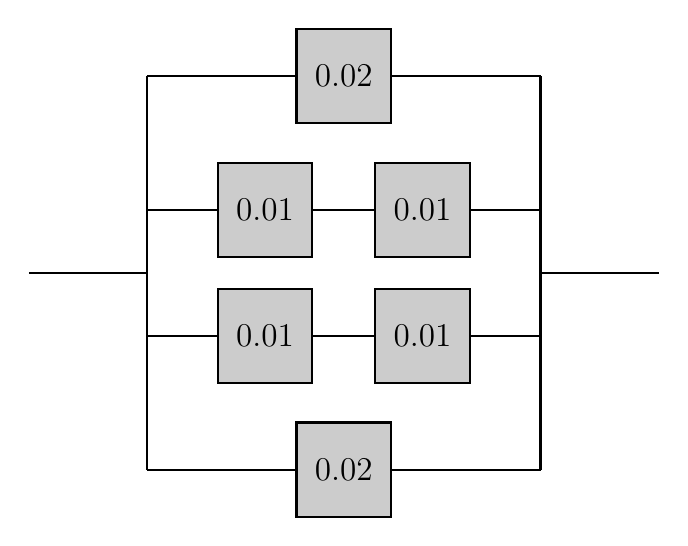
\begin{tikzpicture}[
        thick,
        block/.style={
            rectangle, 
            draw, 
            fill=gray!40, 
            minimum width=1.2cm, 
            minimum height=1.2cm, 
            font=\large
        }
    ]

        % Input and Output lines
        \draw (-1.5, 0) -- (0, 0);
        \draw (5, 0) -- (6.5, 0);

        % Left and Right vertical connection lines
        \draw (0, 2.5) -- (0, -2.5);
        \draw (5, 2.5) -- (5, -2.5);

        % Top Branch
        \node[block] (b1) at (2.5, 2.5) {0.02};
        \draw (0, 2.5) -- (b1.west);
        \draw (b1.east) -- (5, 2.5);

        % Second Branch (from top)
        \node[block] (b2a) at (1.5, 0.8) {0.01};
        \node[block] (b2b) at (3.5, 0.8) {0.01};
        \draw (0, 0.8) -- (b2a.west);
        \draw (b2a.east) -- (b2b.west);
        \draw (b2b.east) -- (5, 0.8);

        % Third Branch (from top)
        \node[block] (b3a) at (1.5, -0.8) {0.01};
        \node[block] (b3b) at (3.5, -0.8) {0.01};
        \draw (0, -0.8) -- (b3a.west);
        \draw (b3a.east) -- (b3b.west);
        \draw (b3b.east) -- (5, -0.8);

        % Bottom Branch
        \node[block] (b4) at (2.5, -2.5) {0.02};
        \draw (0, -2.5) -- (b4.west);
        \draw (b4.east) -- (5, -2.5);

    \end{tikzpicture}
\end{center}
\mk{10} \yr{MATH 245 | L-2/T-1 | 2016--17}

\item A box contains 8 red, 3 white and 9 blue balls. If three balls are drawn at random, determine the probability that:
\begin{enumerate}
  \item all 3 are red.
  \item 2 are red and 1 is white.
  \item at least 1 is white.
\end{enumerate}
\mk{12} \yr{MATH 241 | L-2/T-1 | 2014--15}

\item Three cards are drawn from a deck of 52 cards one after another without replacement. Find the probability that they will come from different suits.
\mk{7} \yr{MATH 241 | L-2/T-1 | 2013--14}

\item The probability that A can solve a problem is $\tfrac{3}{7}$, that B can solve it is $\tfrac{2}{3}$, and that C can solve it is $\tfrac{4}{5}$. If all three try independently, find the probability that the problem will be solved.
\mk{8} \yr{MATH 241 | L-2/T-1 | 2011--12}

\end{enumerate}

%%──────────────────────────────────────────────────────────────────────
\subtopic{cG}{Conditional Probability \& Bayes' Rule}
\label{sub:s8-cond}

\begin{enumerate}\item 500 lottery tickets are sold; 200 pay off at least the cost of the ticket. You buy 5 tickets. Find the probability that you will win back at least the cost of 3 tickets.
\mk{10} \yr{MATH 245 | L-2/T-1 | 2021--22}

\item Delegates arrived by air (0.4), bus (0.2), automobile (0.3), or train (0.1). Among 9 randomly selected delegates, find the probability that 3 arrived by air, 3 by bus, 1 by automobile, and 2 by train.
\mk{10} \yr{MATH 245 | L-2/T-1 | 2021--22}

\item A truth serum has the property that 90\% of the guilty suspects are properly judged while, of course, 10\% of the guilty suspects are improperly found innocent. On the other hand, innocent suspects are misjudged 1\% of the time. If the suspect was selected from a group of suspects of which only 5\%
 have ever committed a crime, and the serum indicates that he is guilty, what is the probability that he is innocent?
\mk{17} \yr{MATH 245 | L-2/T-1 | 2019--20}

\item The probability that a married man watches a TV show is 0.25 and a married woman 0.35. The probability that a man watches given his wife does is 0.8. Find: (i) the probability a married couple watches; (ii) the probability a husband watches given his wife does not.
\mk{13} \yr{MATH 241 | L-2/T-1 | 2015--16}

\end{enumerate}

%%──────────────────────────────────────────────────────────────────────
\subtopic{cG}{Random Variables \& Probability Distributions}
\label{sub:s8-rv}

\begin{enumerate}\item An overseas shipment of 5 automobiles contains 2 with slight paint blemishes. An agency receives 3. Find the probability distribution and $F(x)$ of the number of automobiles with paint blemishes.
\mk{15} \yr{MATH 245 | L-2/T-1 | 2021--22}

\item Each rear tire on an experimental airplane is supposed to be filled to a pressure of 40 psi. Let $X$ and $Y$ denote the actual air pressure for the right and left tires respectively, with joint density function:
\[
f(x,y) = \begin{cases} k(x^{2}+y^{2}), & 30 \le x < 50,\; 30 \le y < 50 \\ 0, & \text{elsewhere} \end{cases}
\]
\begin{enumerate}
  \item Find the value of $k$.
  \item Find $P(30 \le X \le 40 \text{ and } 40 \le Y < 50)$.
  \item Find the probability that both tires are underfilled.
\end{enumerate}
\mk{10} \yr{MATH 245 | L-2/T-1 | 2020--21}

\item The measurement error $X$ of a certain physical quantity has density function:
\[
f(x) = \begin{cases} k(3-x)^{2}, & -1 \le x \le 1 \\ 0, & \text{elsewhere} \end{cases}
\]
\begin{enumerate}
  \item Determine $k$ that renders $f(x)$ a valid density function.
  \item Find the probability that a random error is less than $\tfrac{1}{2}$.
  \item What is the probability that the magnitude of the error exceeds $0.8$?
\end{enumerate}
\mk{10} \yr{MATH 245 | L-2/T-1 | 2020--21}

\item The hospitalization period in days for patients following treatment for a kidney disorder is $Y=X+4$, where $X$ has density:
\[
f(x) = \begin{cases} \dfrac{32}{(x+4)^{3}}, & x > 0 \\ 0, & \text{elsewhere} \end{cases}
\]
Find the average number of days a person is hospitalized following treatment.
\mk{10} \yr{MATH 245 | L-2/T-1 | 2020--21}

\item A continuous random variable $X$ has density $f(x)=e^{-x}$ for $x>0$, $0$ otherwise. Find the expected value of $g(X)=e^{2X/3}$.
\mk{18} \yr{MATH 245 | L-2/T-1 | 2019--20}

\item What is a density function? What conditions must it satisfy? Suppose the distribution function of $X$ is:
\[
F(x)=\begin{cases} 0, & x\le 0 \\ x/8, & 0<x<2 \\ x^{2}/16, & 2\le x<4 \\ 1, & x\ge 4 \end{cases}
\]
\begin{enumerate}
  \item Find the probability density function of $X$.
  \item Find $P(X\ge 1.5)$ and $P(X\ge 1\mid X\le 3)$.
\end{enumerate}
\mk{20} \yr{MATH 245 | L-2/T-1 | 2018--19}

\item A lot containing 7 components is sampled by a quality inspector. The lot contains 4 good and 3 defective components. A sample of 3 is taken. Find the expected value of the number of good components in this sample.
\mk{15} \yr{MATH 245 | L-2/T-1 | 2018--19}

\item A new factory installed 1000 tube lights with a mean life of 120 days and standard deviation 20 days (normally distributed).
\begin{enumerate}
  \item How many tube lights will expire in less than 90 days?
  \item What interval should be allowed between replacements if not more than 10\% should expire before replacement?
\end{enumerate}
\mk{18} \yr{MATH 245 | L-2/T-1 | 2018--19}


% ================= DIAGRAM =================
\begin{center}
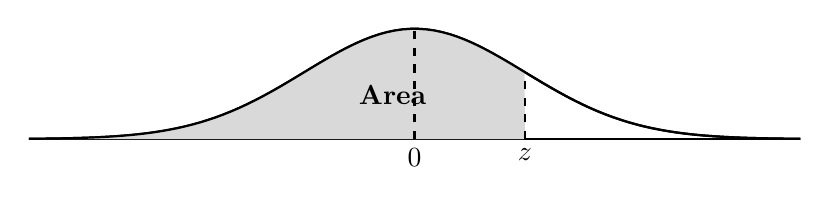
\begin{tikzpicture}[scale=1.4]
    % Draw baseline
    \draw (-3.5,0) -- (3.5,0);
    
    % Draw curve
    \draw[thick, domain=-3.5:3.5, samples=100] plot (\x, {exp(-0.5*\x*\x)});
    
    % Shaded Area from -infinity to z
    \fill[gray!30, domain=-3.5:1.0, samples=100] plot (\x, {exp(-0.5*\x*\x)}) -- (1.0,0) -- (-3.5,0) -- cycle;
    
    % Redraw curve over shading
    \draw[thick, domain=-3.5:3.5, samples=100] plot (\x, {exp(-0.5*\x*\x)});
    
    % Draw center dashed line and z line
    \draw[dashed, thick] (0,0) -- (0,1);
    \draw[dashed, thick] (1.0,0) -- (1.0,{exp(-0.5*1.0*1.0)});
    
    % Add labels
    \node[below] at (0,0) {0};
    \node[below] at (1.0,0) {$z$};
    \node at (-0.2, 0.4) {\textbf{Area}};
\end{tikzpicture}
\end{center}

\vspace{0.3cm}
\noindent\textbf{Table A.3} Areas under the Normal Curve
\vspace{0.2cm}

% ================= COMBINED CONTINUOUS TABLE =================
\begin{center}
\small
\begin{longtable}{ccccccccccc}
\toprule\toprule
$z$ & .00 & .01 & .02 & .03 & .04 & .05 & .06 & .07 & .08 & .09 \\
\midrule
\endhead % This header repeats on every new page

\midrule
\multicolumn{11}{r}{{Continued on next page}} \\
\bottomrule
\endfoot

\bottomrule\bottomrule
\endlastfoot

% --- Negative Z-Scores ---
-3.4 & 0.0003 & 0.0003 & 0.0003 & 0.0003 & 0.0003 & 0.0003 & 0.0003 & 0.0003 & 0.0003 & 0.0002 \\
-3.3 & 0.0005 & 0.0005 & 0.0005 & 0.0004 & 0.0004 & 0.0004 & 0.0004 & 0.0004 & 0.0004 & 0.0003 \\
-3.2 & 0.0007 & 0.0007 & 0.0006 & 0.0006 & 0.0006 & 0.0006 & 0.0006 & 0.0005 & 0.0005 & 0.0005 \\
-3.1 & 0.0010 & 0.0009 & 0.0009 & 0.0009 & 0.0008 & 0.0008 & 0.0008 & 0.0008 & 0.0007 & 0.0007 \\
-3.0 & 0.0013 & 0.0013 & 0.0013 & 0.0012 & 0.0012 & 0.0011 & 0.0011 & 0.0011 & 0.0010 & 0.0010 \\
\addlinespace
-2.9 & 0.0019 & 0.0018 & 0.0017 & 0.0017 & 0.0016 & 0.0016 & 0.0015 & 0.0015 & 0.0014 & 0.0014 \\
-2.8 & 0.0026 & 0.0025 & 0.0024 & 0.0023 & 0.0023 & 0.0022 & 0.0021 & 0.0021 & 0.0020 & 0.0019 \\
-2.7 & 0.0035 & 0.0034 & 0.0033 & 0.0032 & 0.0031 & 0.0030 & 0.0029 & 0.0028 & 0.0027 & 0.0026 \\
-2.6 & 0.0047 & 0.0045 & 0.0044 & 0.0043 & 0.0041 & 0.0040 & 0.0039 & 0.0038 & 0.0037 & 0.0036 \\
-2.5 & 0.0062 & 0.0060 & 0.0059 & 0.0057 & 0.0055 & 0.0054 & 0.0052 & 0.0051 & 0.0049 & 0.0048 \\
\addlinespace
-2.4 & 0.0082 & 0.0080 & 0.0078 & 0.0075 & 0.0073 & 0.0071 & 0.0069 & 0.0068 & 0.0066 & 0.0064 \\
-2.3 & 0.0107 & 0.0104 & 0.0102 & 0.0099 & 0.0096 & 0.0094 & 0.0091 & 0.0089 & 0.0087 & 0.0084 \\
-2.2 & 0.0139 & 0.0136 & 0.0132 & 0.0129 & 0.0125 & 0.0122 & 0.0119 & 0.0116 & 0.0113 & 0.0110 \\
-2.1 & 0.0179 & 0.0174 & 0.0170 & 0.0166 & 0.0162 & 0.0158 & 0.0154 & 0.0150 & 0.0146 & 0.0143 \\
-2.0 & 0.0228 & 0.0222 & 0.0217 & 0.0212 & 0.0207 & 0.0202 & 0.0197 & 0.0192 & 0.0188 & 0.0183 \\
\addlinespace
-1.9 & 0.0287 & 0.0281 & 0.0274 & 0.0268 & 0.0262 & 0.0256 & 0.0250 & 0.0244 & 0.0239 & 0.0233 \\
-1.8 & 0.0359 & 0.0352 & 0.0344 & 0.0336 & 0.0329 & 0.0322 & 0.0314 & 0.0307 & 0.0301 & 0.0294 \\
-1.7 & 0.0446 & 0.0436 & 0.0427 & 0.0418 & 0.0409 & 0.0401 & 0.0392 & 0.0384 & 0.0375 & 0.0367 \\
-1.6 & 0.0548 & 0.0537 & 0.0526 & 0.0516 & 0.0505 & 0.0495 & 0.0485 & 0.0475 & 0.0465 & 0.0455 \\
-1.5 & 0.0668 & 0.0655 & 0.0643 & 0.0630 & 0.0618 & 0.0606 & 0.0594 & 0.0582 & 0.0571 & 0.0559 \\
\addlinespace
-1.4 & 0.0808 & 0.0793 & 0.0778 & 0.0764 & 0.0749 & 0.0735 & 0.0722 & 0.0708 & 0.0694 & 0.0681 \\
-1.3 & 0.0968 & 0.0951 & 0.0934 & 0.0918 & 0.0901 & 0.0885 & 0.0869 & 0.0853 & 0.0838 & 0.0823 \\
-1.2 & 0.1151 & 0.1131 & 0.1112 & 0.1093 & 0.1075 & 0.1056 & 0.1038 & 0.1020 & 0.1003 & 0.0985 \\
-1.1 & 0.1357 & 0.1335 & 0.1314 & 0.1292 & 0.1271 & 0.1251 & 0.1230 & 0.1210 & 0.1190 & 0.1170 \\
-1.0 & 0.1587 & 0.1562 & 0.1539 & 0.1515 & 0.1492 & 0.1469 & 0.1446 & 0.1423 & 0.1401 & 0.1379 \\
\addlinespace
-0.9 & 0.1841 & 0.1814 & 0.1788 & 0.1762 & 0.1736 & 0.1711 & 0.1685 & 0.1660 & 0.1635 & 0.1611 \\
-0.8 & 0.2119 & 0.2090 & 0.2061 & 0.2033 & 0.2005 & 0.1977 & 0.1949 & 0.1922 & 0.1894 & 0.1867 \\
-0.7 & 0.2420 & 0.2389 & 0.2358 & 0.2327 & 0.2296 & 0.2266 & 0.2236 & 0.2206 & 0.2177 & 0.2148 \\
-0.6 & 0.2743 & 0.2709 & 0.2676 & 0.2643 & 0.2611 & 0.2578 & 0.2546 & 0.2514 & 0.2483 & 0.2451 \\
-0.5 & 0.3085 & 0.3050 & 0.3015 & 0.2981 & 0.2946 & 0.2912 & 0.2877 & 0.2843 & 0.2810 & 0.2776 \\
\addlinespace
-0.4 & 0.3446 & 0.3409 & 0.3372 & 0.3336 & 0.3300 & 0.3264 & 0.3228 & 0.3192 & 0.3156 & 0.3121 \\
-0.3 & 0.3821 & 0.3783 & 0.3745 & 0.3707 & 0.3669 & 0.3632 & 0.3594 & 0.3557 & 0.3520 & 0.3483 \\
-0.2 & 0.4207 & 0.4168 & 0.4129 & 0.4090 & 0.4052 & 0.4013 & 0.3974 & 0.3936 & 0.3897 & 0.3859 \\
-0.1 & 0.4602 & 0.4562 & 0.4522 & 0.4483 & 0.4443 & 0.4404 & 0.4364 & 0.4325 & 0.4286 & 0.4247 \\
-0.0 & 0.5000 & 0.4960 & 0.4920 & 0.4880 & 0.4840 & 0.4801 & 0.4761 & 0.4721 & 0.4681 & 0.4641 \\
\midrule
% --- Positive Z-Scores ---
0.0 & 0.5000 & 0.5040 & 0.5080 & 0.5120 & 0.5160 & 0.5199 & 0.5239 & 0.5279 & 0.5319 & 0.5359 \\
0.1 & 0.5398 & 0.5438 & 0.5478 & 0.5517 & 0.5557 & 0.5596 & 0.5636 & 0.5675 & 0.5714 & 0.5753 \\
0.2 & 0.5793 & 0.5832 & 0.5871 & 0.5910 & 0.5948 & 0.5987 & 0.6026 & 0.6064 & 0.6103 & 0.6141 \\
0.3 & 0.6179 & 0.6217 & 0.6255 & 0.6293 & 0.6331 & 0.6368 & 0.6406 & 0.6443 & 0.6480 & 0.6517 \\
0.4 & 0.6554 & 0.6591 & 0.6628 & 0.6664 & 0.6700 & 0.6736 & 0.6772 & 0.6808 & 0.6844 & 0.6879 \\
\addlinespace
0.5 & 0.6915 & 0.6950 & 0.6985 & 0.7019 & 0.7054 & 0.7088 & 0.7123 & 0.7157 & 0.7190 & 0.7224 \\
0.6 & 0.7257 & 0.7291 & 0.7324 & 0.7357 & 0.7389 & 0.7422 & 0.7454 & 0.7486 & 0.7517 & 0.7549 \\
0.7 & 0.7580 & 0.7611 & 0.7642 & 0.7673 & 0.7704 & 0.7734 & 0.7764 & 0.7794 & 0.7823 & 0.7852 \\
0.8 & 0.7881 & 0.7910 & 0.7939 & 0.7967 & 0.7995 & 0.8023 & 0.8051 & 0.8078 & 0.8106 & 0.8133 \\
0.9 & 0.8159 & 0.8186 & 0.8212 & 0.8238 & 0.8264 & 0.8289 & 0.8315 & 0.8340 & 0.8365 & 0.8389 \\
\addlinespace
1.0 & 0.8413 & 0.8438 & 0.8461 & 0.8485 & 0.8508 & 0.8531 & 0.8554 & 0.8577 & 0.8599 & 0.8621 \\
1.1 & 0.8643 & 0.8665 & 0.8686 & 0.8708 & 0.8729 & 0.8749 & 0.8770 & 0.8790 & 0.8810 & 0.8830 \\
1.2 & 0.8849 & 0.8869 & 0.8888 & 0.8907 & 0.8925 & 0.8944 & 0.8962 & 0.8980 & 0.8997 & 0.9015 \\
1.3 & 0.9032 & 0.9049 & 0.9066 & 0.9082 & 0.9099 & 0.9115 & 0.9131 & 0.9147 & 0.9162 & 0.9177 \\
1.4 & 0.9192 & 0.9207 & 0.9222 & 0.9236 & 0.9251 & 0.9265 & 0.9278 & 0.9292 & 0.9306 & 0.9319 \\
\addlinespace
1.5 & 0.9332 & 0.9345 & 0.9357 & 0.9370 & 0.9382 & 0.9394 & 0.9406 & 0.9418 & 0.9429 & 0.9441 \\
1.6 & 0.9452 & 0.9463 & 0.9474 & 0.9484 & 0.9495 & 0.9505 & 0.9515 & 0.9525 & 0.9535 & 0.9545 \\
1.7 & 0.9554 & 0.9564 & 0.9573 & 0.9582 & 0.9591 & 0.9599 & 0.9608 & 0.9616 & 0.9625 & 0.9633 \\
1.8 & 0.9641 & 0.9649 & 0.9656 & 0.9664 & 0.9671 & 0.9678 & 0.9686 & 0.9693 & 0.9699 & 0.9706 \\
1.9 & 0.9713 & 0.9719 & 0.9726 & 0.9732 & 0.9738 & 0.9744 & 0.9750 & 0.9756 & 0.9761 & 0.9767 \\
\addlinespace
2.0 & 0.9772 & 0.9778 & 0.9783 & 0.9788 & 0.9793 & 0.9798 & 0.9803 & 0.9808 & 0.9812 & 0.9817 \\
2.1 & 0.9821 & 0.9826 & 0.9830 & 0.9834 & 0.9838 & 0.9842 & 0.9846 & 0.9850 & 0.9854 & 0.9857 \\
2.2 & 0.9861 & 0.9864 & 0.9868 & 0.9871 & 0.9875 & 0.9878 & 0.9881 & 0.9884 & 0.9887 & 0.9890 \\
2.3 & 0.9893 & 0.9896 & 0.9898 & 0.9901 & 0.9904 & 0.9906 & 0.9909 & 0.9911 & 0.9913 & 0.9916 \\
2.4 & 0.9918 & 0.9920 & 0.9922 & 0.9925 & 0.9927 & 0.9929 & 0.9931 & 0.9932 & 0.9934 & 0.9936 \\
\addlinespace
2.5 & 0.9938 & 0.9940 & 0.9941 & 0.9943 & 0.9945 & 0.9946 & 0.9948 & 0.9949 & 0.9951 & 0.9952 \\
2.6 & 0.9953 & 0.9955 & 0.9956 & 0.9957 & 0.9959 & 0.9960 & 0.9961 & 0.9962 & 0.9963 & 0.9964 \\
2.7 & 0.9965 & 0.9966 & 0.9967 & 0.9968 & 0.9969 & 0.9970 & 0.9971 & 0.9972 & 0.9973 & 0.9974 \\
2.8 & 0.9974 & 0.9975 & 0.9976 & 0.9977 & 0.9977 & 0.9978 & 0.9979 & 0.9979 & 0.9980 & 0.9981 \\
2.9 & 0.9981 & 0.9982 & 0.9982 & 0.9983 & 0.9984 & 0.9984 & 0.9985 & 0.9985 & 0.9986 & 0.9986 \\
\addlinespace
3.0 & 0.9987 & 0.9987 & 0.9987 & 0.9987 & 0.9988 & 0.9988 & 0.9989 & 0.9989 & 0.9990 & 0.9990 \\
3.1 & 0.9990 & 0.9991 & 0.9991 & 0.9991 & 0.9992 & 0.9992 & 0.9992 & 0.9992 & 0.9993 & 0.9993 \\
3.2 & 0.9993 & 0.9993 & 0.9994 & 0.9994 & 0.9994 & 0.9994 & 0.9994 & 0.9995 & 0.9995 & 0.9995 \\
3.3 & 0.9995 & 0.9995 & 0.9995 & 0.9996 & 0.9996 & 0.9996 & 0.9996 & 0.9996 & 0.9996 & 0.9997 \\
3.4 & 0.9997 & 0.9997 & 0.9997 & 0.9997 & 0.9997 & 0.9997 & 0.9997 & 0.9997 & 0.9997 & 0.9998 \\
\end{longtable}
\end{center}

\item A U-shaped component is formed from three parts A, B, and C. The length of A is normally distributed with mean 10 mm and standard deviation 0.1 mm. The thickness of parts B and C is normally distributed with mean 2 mm and standard deviation 0.05 mm. Assume all dimensions are independent.
\begin{enumerate}
  \item Determine the mean and standard deviation of the length of the gap $D$.
  \item What is the probability that the gap $D$ is less than 5.9 mm?(Necessary table attached)
\end{enumerate}
\begin{center}
  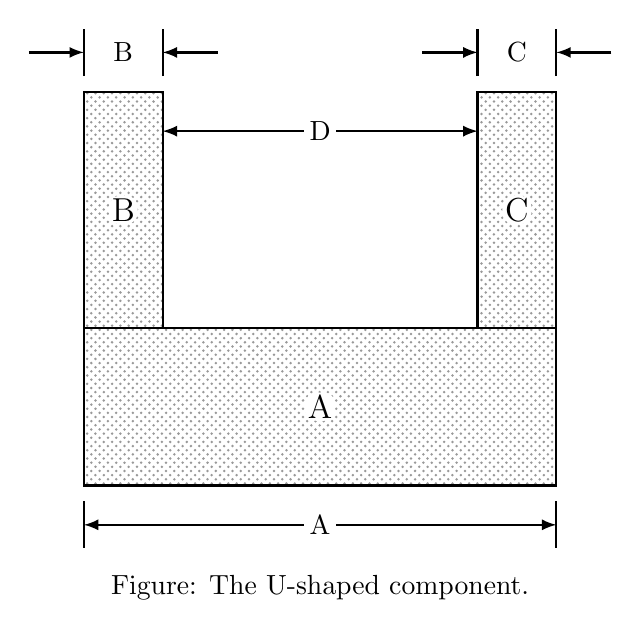
\begin{tikzpicture}[
        thick,
        component/.style={
            draw, 
            pattern=crosshatch dots, 
            pattern color=gray!80,
            text=black
        }
    ]

        % Draw the three rectangular blocks
        % Bottom block
        \draw[component] (0,0) rectangle (6,2);
        \node[fill=white, inner sep=1pt, rounded corners] at (3, 1) {\large A};
        
        % Left vertical arm
        \draw[component] (0,2) rectangle (1,5);
        \node[fill=white, inner sep=1pt, rounded corners] at (0.5, 3.5) {\large B};
        
        % Right vertical arm
        \draw[component] (5,2) rectangle (6,5);
        \node[fill=white, inner sep=1pt, rounded corners] at (5.5, 3.5) {\large C};

        % Dimension lines
        
        % Dimension A (Bottom)
        \draw (0, -0.2) -- (0, -0.8);
        \draw (6, -0.2) -- (6, -0.8);
        \draw[latex-latex] (0, -0.5) -- (6, -0.5) node[midway, fill=white, inner sep=2pt] {A};
        
        % Dimension B (Top Left)
        \draw (0, 5.2) -- (0, 5.8);
        \draw (1, 5.2) -- (1, 5.8);
        \draw[-latex] (-0.7, 5.5) -- (0, 5.5);
        \draw[-latex] (1.7, 5.5) -- (1, 5.5);
        \node at (0.5, 5.5) {B};
        
        % Dimension C (Top Right)
        \draw (5, 5.2) -- (5, 5.8);
        \draw (6, 5.2) -- (6, 5.8);
        \draw[-latex] (4.3, 5.5) -- (5, 5.5);
        \draw[-latex] (6.7, 5.5) -- (6, 5.5);
        \node at (5.5, 5.5) {C};
        
        % Dimension D (Inner width)
        \draw[latex-latex] (1, 4.5) -- (5, 4.5) node[midway, fill=white, inner sep=2pt] {D};

        % Figure Caption
        \node at (3, -1.3) {Figure: The U-shaped component.};

    \end{tikzpicture}
\end{center}
\mk{10} \yr{MATH 245 | L-2/T-1 | 2016--17}


% ================= NORMAL DISTRIBUTION DIAGRAM =================
\begin{center}
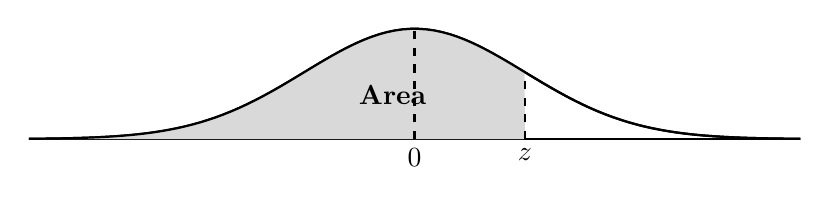
\begin{tikzpicture}[scale=1.4]
    % Draw baseline
    \draw (-3.5,0) -- (3.5,0);
    
    % Draw curve
    \draw[thick, domain=-3.5:3.5, samples=100] plot (\x, {exp(-0.5*\x*\x)});
    
    % Shaded Area from -infinity to z (positive z side)
    \fill[gray!30, domain=-3.5:1.0, samples=100] plot (\x, {exp(-0.5*\x*\x)}) -- (1.0,0) -- (-3.5,0) -- cycle;
    
    % Redraw curve over shading to keep the line crisp
    \draw[thick, domain=-3.5:3.5, samples=100] plot (\x, {exp(-0.5*\x*\x)});
    
    % Draw center dashed line and z line
    \draw[dashed, thick] (0,0) -- (0,1);
    \draw[dashed, thick] (1.0,0) -- (1.0,{exp(-0.5*1.0*1.0)});
    
    % Add labels
    \node[below] at (0,0) {0};
    \node[below] at (1.0,0) {$z$};
    \node at (-0.2, 0.4) {\textbf{Area}};
\end{tikzpicture}
\end{center}

\vspace{0.3cm}
\noindent\textbf{Table A.3 (continued)} Areas under the Normal Curve
\vspace{0.2cm}

% ================= DATA TABLE =================
\begin{center}
\small
\begin{longtable}{ccccccccccc}
\toprule\toprule
$z$ & .00 & .01 & .02 & .03 & .04 & .05 & .06 & .07 & .08 & .09 \\
\midrule
\endhead
\bottomrule\bottomrule
\endfoot
0.0 & 0.5000 & 0.5040 & 0.5080 & 0.5120 & 0.5160 & 0.5199 & 0.5239 & 0.5279 & 0.5319 & 0.5359 \\
0.1 & 0.5398 & 0.5438 & 0.5478 & 0.5517 & 0.5557 & 0.5596 & 0.5636 & 0.5675 & 0.5714 & 0.5753 \\
0.2 & 0.5793 & 0.5832 & 0.5871 & 0.5910 & 0.5948 & 0.5987 & 0.6026 & 0.6064 & 0.6103 & 0.6141 \\
0.3 & 0.6179 & 0.6217 & 0.6255 & 0.6293 & 0.6331 & 0.6368 & 0.6406 & 0.6443 & 0.6480 & 0.6517 \\
0.4 & 0.6554 & 0.6591 & 0.6628 & 0.6664 & 0.6700 & 0.6736 & 0.6772 & 0.6808 & 0.6844 & 0.6879 \\
0.5 & 0.6915 & 0.6950 & 0.6985 & 0.7019 & 0.7054 & 0.7088 & 0.7123 & 0.7157 & 0.7190 & 0.7224 \\
0.6 & 0.7257 & 0.7291 & 0.7324 & 0.7357 & 0.7389 & 0.7422 & 0.7454 & 0.7486 & 0.7517 & 0.7549 \\
0.7 & 0.7580 & 0.7611 & 0.7642 & 0.7673 & 0.7704 & 0.7734 & 0.7764 & 0.7794 & 0.7823 & 0.7852 \\
0.8 & 0.7881 & 0.7910 & 0.7939 & 0.7967 & 0.7995 & 0.8023 & 0.8051 & 0.8078 & 0.8106 & 0.8133 \\
0.9 & 0.8159 & 0.8186 & 0.8212 & 0.8238 & 0.8264 & 0.8289 & 0.8315 & 0.8340 & 0.8365 & 0.8389 \\
1.0 & 0.8413 & 0.8438 & 0.8461 & 0.8485 & 0.8508 & 0.8531 & 0.8554 & 0.8577 & 0.8599 & 0.8621 \\
1.1 & 0.8643 & 0.8665 & 0.8686 & 0.8708 & 0.8729 & 0.8749 & 0.8770 & 0.8790 & 0.8810 & 0.8830 \\
1.2 & 0.8849 & 0.8869 & 0.8888 & 0.8907 & 0.8925 & 0.8944 & 0.8962 & 0.8980 & 0.8997 & 0.9015 \\
1.3 & 0.9032 & 0.9049 & 0.9066 & 0.9082 & 0.9099 & 0.9115 & 0.9131 & 0.9147 & 0.9162 & 0.9177 \\
1.4 & 0.9192 & 0.9207 & 0.9222 & 0.9236 & 0.9251 & 0.9265 & 0.9278 & 0.9292 & 0.9306 & 0.9319 \\
1.5 & 0.9332 & 0.9345 & 0.9357 & 0.9370 & 0.9382 & 0.9394 & 0.9406 & 0.9418 & 0.9429 & 0.9441 \\
1.6 & 0.9452 & 0.9463 & 0.9474 & 0.9484 & 0.9495 & 0.9505 & 0.9515 & 0.9525 & 0.9535 & 0.9545 \\
1.7 & 0.9554 & 0.9564 & 0.9573 & 0.9582 & 0.9591 & 0.9599 & 0.9608 & 0.9616 & 0.9625 & 0.9633 \\
1.8 & 0.9641 & 0.9649 & 0.9656 & 0.9664 & 0.9671 & 0.9678 & 0.9686 & 0.9693 & 0.9699 & 0.9706 \\
1.9 & 0.9713 & 0.9719 & 0.9726 & 0.9732 & 0.9738 & 0.9744 & 0.9750 & 0.9756 & 0.9761 & 0.9767 \\
2.0 & 0.9772 & 0.9778 & 0.9783 & 0.9788 & 0.9793 & 0.9798 & 0.9803 & 0.9808 & 0.9812 & 0.9817 \\
2.1 & 0.9821 & 0.9826 & 0.9830 & 0.9834 & 0.9838 & 0.9842 & 0.9846 & 0.9850 & 0.9854 & 0.9857 \\
2.2 & 0.9861 & 0.9864 & 0.9868 & 0.9871 & 0.9875 & 0.9878 & 0.9881 & 0.9884 & 0.9887 & 0.9890 \\
2.3 & 0.9893 & 0.9896 & 0.9898 & 0.9901 & 0.9904 & 0.9906 & 0.9909 & 0.9911 & 0.9913 & 0.9916 \\
2.4 & 0.9918 & 0.9920 & 0.9922 & 0.9925 & 0.9927 & 0.9929 & 0.9931 & 0.9932 & 0.9934 & 0.9936 \\
2.5 & 0.9938 & 0.9940 & 0.9941 & 0.9943 & 0.9945 & 0.9946 & 0.9948 & 0.9949 & 0.9951 & 0.9952 \\
2.6 & 0.9953 & 0.9955 & 0.9956 & 0.9957 & 0.9959 & 0.9960 & 0.9961 & 0.9962 & 0.9963 & 0.9964 \\
2.7 & 0.9965 & 0.9966 & 0.9967 & 0.9968 & 0.9969 & 0.9970 & 0.9971 & 0.9972 & 0.9973 & 0.9974 \\
2.8 & 0.9974 & 0.9975 & 0.9976 & 0.9977 & 0.9977 & 0.9978 & 0.9979 & 0.9979 & 0.9980 & 0.9981 \\
2.9 & 0.9981 & 0.9982 & 0.9982 & 0.9983 & 0.9984 & 0.9984 & 0.9985 & 0.9985 & 0.9986 & 0.9986 \\
3.0 & 0.9987 & 0.9987 & 0.9987 & 0.9987 & 0.9988 & 0.9988 & 0.9989 & 0.9989 & 0.9990 & 0.9990 \\
3.1 & 0.9990 & 0.9991 & 0.9991 & 0.9991 & 0.9992 & 0.9992 & 0.9992 & 0.9992 & 0.9993 & 0.9993 \\
3.2 & 0.9993 & 0.9993 & 0.9994 & 0.9994 & 0.9994 & 0.9994 & 0.9994 & 0.9995 & 0.9995 & 0.9995 \\
3.3 & 0.9995 & 0.9995 & 0.9995 & 0.9996 & 0.9996 & 0.9996 & 0.9996 & 0.9996 & 0.9996 & 0.9997 \\
3.4 & 0.9997 & 0.9997 & 0.9997 & 0.9997 & 0.9997 & 0.9997 & 0.9997 & 0.9997 & 0.9997 & 0.9998 \\
\end{longtable}
\end{center}

\item The probability that an entering college student will graduate is $0.4$. Determine the probability that out of 5 students:
\begin{enumerate}
  \item none will graduate.
  \item at least 1 will graduate.
  \item all will graduate.
\end{enumerate}
\mk{12} \yr{MATH 241 | L-2/T-1 | 2014--15}

\item A workshop produces 2000 units per day. The average weight of units is 130 kg with a standard deviation of 10 kg. Assuming normal distribution, how many units are expected to weigh less than 142 kg?
\mk{11} \yr{MATH 241 | L-2/T-1 | 2014--15}

\begin{center}
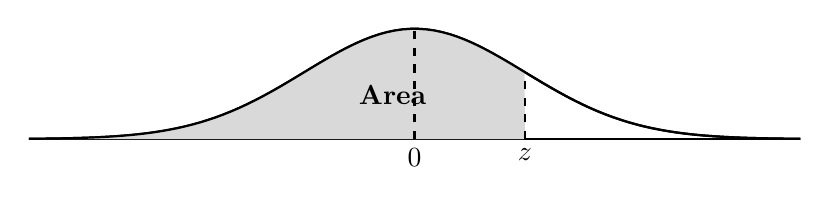
\begin{tikzpicture}[scale=1.4]
    % Draw baseline
    \draw (-3.5,0) -- (3.5,0);
    
    % Draw curve
    \draw[thick, domain=-3.5:3.5, samples=100] plot (\x, {exp(-0.5*\x*\x)});
    
    % Shaded Area from -infinity to z
    \fill[gray!30, domain=-3.5:1.0, samples=100] plot (\x, {exp(-0.5*\x*\x)}) -- (1.0,0) -- (-3.5,0) -- cycle;
    
    % Redraw curve over shading
    \draw[thick, domain=-3.5:3.5, samples=100] plot (\x, {exp(-0.5*\x*\x)});
    
    % Draw center dashed line and z line
    \draw[dashed, thick] (0,0) -- (0,1);
    \draw[dashed, thick] (1.0,0) -- (1.0,{exp(-0.5*1.0*1.0)});
    
    % Add labels
    \node[below] at (0,0) {0};
    \node[below] at (1.0,0) {$z$};
    \node at (-0.2, 0.4) {\textbf{Area}};
\end{tikzpicture}
\end{center}

\vspace{0.3cm}
\noindent\textbf{Table A.3} Areas under the Normal Curve
\vspace{0.2cm}

% ================= COMBINED CONTINUOUS TABLE =================
\begin{center}
\small
\begin{longtable}{ccccccccccc}
\toprule\toprule
$z$ & .00 & .01 & .02 & .03 & .04 & .05 & .06 & .07 & .08 & .09 \\
\midrule
\endhead % This header repeats on every new page

\midrule
\multicolumn{11}{r}{{Continued on next page}} \\
\bottomrule
\endfoot

\bottomrule\bottomrule
\endlastfoot

% --- Negative Z-Scores ---
-3.4 & 0.0003 & 0.0003 & 0.0003 & 0.0003 & 0.0003 & 0.0003 & 0.0003 & 0.0003 & 0.0003 & 0.0002 \\
-3.3 & 0.0005 & 0.0005 & 0.0005 & 0.0004 & 0.0004 & 0.0004 & 0.0004 & 0.0004 & 0.0004 & 0.0003 \\
-3.2 & 0.0007 & 0.0007 & 0.0006 & 0.0006 & 0.0006 & 0.0006 & 0.0006 & 0.0005 & 0.0005 & 0.0005 \\
-3.1 & 0.0010 & 0.0009 & 0.0009 & 0.0009 & 0.0008 & 0.0008 & 0.0008 & 0.0008 & 0.0007 & 0.0007 \\
-3.0 & 0.0013 & 0.0013 & 0.0013 & 0.0012 & 0.0012 & 0.0011 & 0.0011 & 0.0011 & 0.0010 & 0.0010 \\
\addlinespace
-2.9 & 0.0019 & 0.0018 & 0.0017 & 0.0017 & 0.0016 & 0.0016 & 0.0015 & 0.0015 & 0.0014 & 0.0014 \\
-2.8 & 0.0026 & 0.0025 & 0.0024 & 0.0023 & 0.0023 & 0.0022 & 0.0021 & 0.0021 & 0.0020 & 0.0019 \\
-2.7 & 0.0035 & 0.0034 & 0.0033 & 0.0032 & 0.0031 & 0.0030 & 0.0029 & 0.0028 & 0.0027 & 0.0026 \\
-2.6 & 0.0047 & 0.0045 & 0.0044 & 0.0043 & 0.0041 & 0.0040 & 0.0039 & 0.0038 & 0.0037 & 0.0036 \\
-2.5 & 0.0062 & 0.0060 & 0.0059 & 0.0057 & 0.0055 & 0.0054 & 0.0052 & 0.0051 & 0.0049 & 0.0048 \\
\addlinespace
-2.4 & 0.0082 & 0.0080 & 0.0078 & 0.0075 & 0.0073 & 0.0071 & 0.0069 & 0.0068 & 0.0066 & 0.0064 \\
-2.3 & 0.0107 & 0.0104 & 0.0102 & 0.0099 & 0.0096 & 0.0094 & 0.0091 & 0.0089 & 0.0087 & 0.0084 \\
-2.2 & 0.0139 & 0.0136 & 0.0132 & 0.0129 & 0.0125 & 0.0122 & 0.0119 & 0.0116 & 0.0113 & 0.0110 \\
-2.1 & 0.0179 & 0.0174 & 0.0170 & 0.0166 & 0.0162 & 0.0158 & 0.0154 & 0.0150 & 0.0146 & 0.0143 \\
-2.0 & 0.0228 & 0.0222 & 0.0217 & 0.0212 & 0.0207 & 0.0202 & 0.0197 & 0.0192 & 0.0188 & 0.0183 \\
\addlinespace
-1.9 & 0.0287 & 0.0281 & 0.0274 & 0.0268 & 0.0262 & 0.0256 & 0.0250 & 0.0244 & 0.0239 & 0.0233 \\
-1.8 & 0.0359 & 0.0352 & 0.0344 & 0.0336 & 0.0329 & 0.0322 & 0.0314 & 0.0307 & 0.0301 & 0.0294 \\
-1.7 & 0.0446 & 0.0436 & 0.0427 & 0.0418 & 0.0409 & 0.0401 & 0.0392 & 0.0384 & 0.0375 & 0.0367 \\
-1.6 & 0.0548 & 0.0537 & 0.0526 & 0.0516 & 0.0505 & 0.0495 & 0.0485 & 0.0475 & 0.0465 & 0.0455 \\
-1.5 & 0.0668 & 0.0655 & 0.0643 & 0.0630 & 0.0618 & 0.0606 & 0.0594 & 0.0582 & 0.0571 & 0.0559 \\
\addlinespace
-1.4 & 0.0808 & 0.0793 & 0.0778 & 0.0764 & 0.0749 & 0.0735 & 0.0722 & 0.0708 & 0.0694 & 0.0681 \\
-1.3 & 0.0968 & 0.0951 & 0.0934 & 0.0918 & 0.0901 & 0.0885 & 0.0869 & 0.0853 & 0.0838 & 0.0823 \\
-1.2 & 0.1151 & 0.1131 & 0.1112 & 0.1093 & 0.1075 & 0.1056 & 0.1038 & 0.1020 & 0.1003 & 0.0985 \\
-1.1 & 0.1357 & 0.1335 & 0.1314 & 0.1292 & 0.1271 & 0.1251 & 0.1230 & 0.1210 & 0.1190 & 0.1170 \\
-1.0 & 0.1587 & 0.1562 & 0.1539 & 0.1515 & 0.1492 & 0.1469 & 0.1446 & 0.1423 & 0.1401 & 0.1379 \\
\addlinespace
-0.9 & 0.1841 & 0.1814 & 0.1788 & 0.1762 & 0.1736 & 0.1711 & 0.1685 & 0.1660 & 0.1635 & 0.1611 \\
-0.8 & 0.2119 & 0.2090 & 0.2061 & 0.2033 & 0.2005 & 0.1977 & 0.1949 & 0.1922 & 0.1894 & 0.1867 \\
-0.7 & 0.2420 & 0.2389 & 0.2358 & 0.2327 & 0.2296 & 0.2266 & 0.2236 & 0.2206 & 0.2177 & 0.2148 \\
-0.6 & 0.2743 & 0.2709 & 0.2676 & 0.2643 & 0.2611 & 0.2578 & 0.2546 & 0.2514 & 0.2483 & 0.2451 \\
-0.5 & 0.3085 & 0.3050 & 0.3015 & 0.2981 & 0.2946 & 0.2912 & 0.2877 & 0.2843 & 0.2810 & 0.2776 \\
\addlinespace
-0.4 & 0.3446 & 0.3409 & 0.3372 & 0.3336 & 0.3300 & 0.3264 & 0.3228 & 0.3192 & 0.3156 & 0.3121 \\
-0.3 & 0.3821 & 0.3783 & 0.3745 & 0.3707 & 0.3669 & 0.3632 & 0.3594 & 0.3557 & 0.3520 & 0.3483 \\
-0.2 & 0.4207 & 0.4168 & 0.4129 & 0.4090 & 0.4052 & 0.4013 & 0.3974 & 0.3936 & 0.3897 & 0.3859 \\
-0.1 & 0.4602 & 0.4562 & 0.4522 & 0.4483 & 0.4443 & 0.4404 & 0.4364 & 0.4325 & 0.4286 & 0.4247 \\
-0.0 & 0.5000 & 0.4960 & 0.4920 & 0.4880 & 0.4840 & 0.4801 & 0.4761 & 0.4721 & 0.4681 & 0.4641 \\
\midrule
% --- Positive Z-Scores ---
0.0 & 0.5000 & 0.5040 & 0.5080 & 0.5120 & 0.5160 & 0.5199 & 0.5239 & 0.5279 & 0.5319 & 0.5359 \\
0.1 & 0.5398 & 0.5438 & 0.5478 & 0.5517 & 0.5557 & 0.5596 & 0.5636 & 0.5675 & 0.5714 & 0.5753 \\
0.2 & 0.5793 & 0.5832 & 0.5871 & 0.5910 & 0.5948 & 0.5987 & 0.6026 & 0.6064 & 0.6103 & 0.6141 \\
0.3 & 0.6179 & 0.6217 & 0.6255 & 0.6293 & 0.6331 & 0.6368 & 0.6406 & 0.6443 & 0.6480 & 0.6517 \\
0.4 & 0.6554 & 0.6591 & 0.6628 & 0.6664 & 0.6700 & 0.6736 & 0.6772 & 0.6808 & 0.6844 & 0.6879 \\
\addlinespace
0.5 & 0.6915 & 0.6950 & 0.6985 & 0.7019 & 0.7054 & 0.7088 & 0.7123 & 0.7157 & 0.7190 & 0.7224 \\
0.6 & 0.7257 & 0.7291 & 0.7324 & 0.7357 & 0.7389 & 0.7422 & 0.7454 & 0.7486 & 0.7517 & 0.7549 \\
0.7 & 0.7580 & 0.7611 & 0.7642 & 0.7673 & 0.7704 & 0.7734 & 0.7764 & 0.7794 & 0.7823 & 0.7852 \\
0.8 & 0.7881 & 0.7910 & 0.7939 & 0.7967 & 0.7995 & 0.8023 & 0.8051 & 0.8078 & 0.8106 & 0.8133 \\
0.9 & 0.8159 & 0.8186 & 0.8212 & 0.8238 & 0.8264 & 0.8289 & 0.8315 & 0.8340 & 0.8365 & 0.8389 \\
\addlinespace
1.0 & 0.8413 & 0.8438 & 0.8461 & 0.8485 & 0.8508 & 0.8531 & 0.8554 & 0.8577 & 0.8599 & 0.8621 \\
1.1 & 0.8643 & 0.8665 & 0.8686 & 0.8708 & 0.8729 & 0.8749 & 0.8770 & 0.8790 & 0.8810 & 0.8830 \\
1.2 & 0.8849 & 0.8869 & 0.8888 & 0.8907 & 0.8925 & 0.8944 & 0.8962 & 0.8980 & 0.8997 & 0.9015 \\
1.3 & 0.9032 & 0.9049 & 0.9066 & 0.9082 & 0.9099 & 0.9115 & 0.9131 & 0.9147 & 0.9162 & 0.9177 \\
1.4 & 0.9192 & 0.9207 & 0.9222 & 0.9236 & 0.9251 & 0.9265 & 0.9278 & 0.9292 & 0.9306 & 0.9319 \\
\addlinespace
1.5 & 0.9332 & 0.9345 & 0.9357 & 0.9370 & 0.9382 & 0.9394 & 0.9406 & 0.9418 & 0.9429 & 0.9441 \\
1.6 & 0.9452 & 0.9463 & 0.9474 & 0.9484 & 0.9495 & 0.9505 & 0.9515 & 0.9525 & 0.9535 & 0.9545 \\
1.7 & 0.9554 & 0.9564 & 0.9573 & 0.9582 & 0.9591 & 0.9599 & 0.9608 & 0.9616 & 0.9625 & 0.9633 \\
1.8 & 0.9641 & 0.9649 & 0.9656 & 0.9664 & 0.9671 & 0.9678 & 0.9686 & 0.9693 & 0.9699 & 0.9706 \\
1.9 & 0.9713 & 0.9719 & 0.9726 & 0.9732 & 0.9738 & 0.9744 & 0.9750 & 0.9756 & 0.9761 & 0.9767 \\
\addlinespace
2.0 & 0.9772 & 0.9778 & 0.9783 & 0.9788 & 0.9793 & 0.9798 & 0.9803 & 0.9808 & 0.9812 & 0.9817 \\
2.1 & 0.9821 & 0.9826 & 0.9830 & 0.9834 & 0.9838 & 0.9842 & 0.9846 & 0.9850 & 0.9854 & 0.9857 \\
2.2 & 0.9861 & 0.9864 & 0.9868 & 0.9871 & 0.9875 & 0.9878 & 0.9881 & 0.9884 & 0.9887 & 0.9890 \\
2.3 & 0.9893 & 0.9896 & 0.9898 & 0.9901 & 0.9904 & 0.9906 & 0.9909 & 0.9911 & 0.9913 & 0.9916 \\
2.4 & 0.9918 & 0.9920 & 0.9922 & 0.9925 & 0.9927 & 0.9929 & 0.9931 & 0.9932 & 0.9934 & 0.9936 \\
\addlinespace
2.5 & 0.9938 & 0.9940 & 0.9941 & 0.9943 & 0.9945 & 0.9946 & 0.9948 & 0.9949 & 0.9951 & 0.9952 \\
2.6 & 0.9953 & 0.9955 & 0.9956 & 0.9957 & 0.9959 & 0.9960 & 0.9961 & 0.9962 & 0.9963 & 0.9964 \\
2.7 & 0.9965 & 0.9966 & 0.9967 & 0.9968 & 0.9969 & 0.9970 & 0.9971 & 0.9972 & 0.9973 & 0.9974 \\
2.8 & 0.9974 & 0.9975 & 0.9976 & 0.9977 & 0.9977 & 0.9978 & 0.9979 & 0.9979 & 0.9980 & 0.9981 \\
2.9 & 0.9981 & 0.9982 & 0.9982 & 0.9983 & 0.9984 & 0.9984 & 0.9985 & 0.9985 & 0.9986 & 0.9986 \\
\addlinespace
3.0 & 0.9987 & 0.9987 & 0.9987 & 0.9987 & 0.9988 & 0.9988 & 0.9989 & 0.9989 & 0.9990 & 0.9990 \\
3.1 & 0.9990 & 0.9991 & 0.9991 & 0.9991 & 0.9992 & 0.9992 & 0.9992 & 0.9992 & 0.9993 & 0.9993 \\
3.2 & 0.9993 & 0.9993 & 0.9994 & 0.9994 & 0.9994 & 0.9994 & 0.9994 & 0.9995 & 0.9995 & 0.9995 \\
3.3 & 0.9995 & 0.9995 & 0.9995 & 0.9996 & 0.9996 & 0.9996 & 0.9996 & 0.9996 & 0.9996 & 0.9997 \\
3.4 & 0.9997 & 0.9997 & 0.9997 & 0.9997 & 0.9997 & 0.9997 & 0.9997 & 0.9997 & 0.9997 & 0.9998 \\
\end{longtable}
\end{center}

\item If $10\%$ of the instruments produced by a company are defective, find the probability that out of 12 instruments, at least 4 will be defective.
\mk{8} \yr{MATH 241 | L-2/T-1 | 2013--14}

\item In testing a certain kind of truck tire over rugged terrain, $20\%$ of the trucks fail to complete the test run without a blowout. Of the next 18 trucks tested, find the probability (using both binomial and Poisson distribution) that:
\begin{enumerate}
  \item from 4 to 7 have blowouts.
  \item fewer than 3 have blowouts.
  \item more than 5 have blowouts.
\end{enumerate}
\mk{10} \yr{MATH 241 | L-2/T-1 | 2012--13}

\item Derive the mean and variance of the frequency function for the binomial distribution.
mk{10} \yr{MATH 241 | L-2/T-1 | 2012--13}

\item For the joint density function:
\[
f(x,y) = \begin{cases} \dfrac{6-x-y}{8}, & 0<x<2,\; 2<y<4 \\ 0, & \text{elsewhere} \end{cases}
\]
Find $P(1<Y<3\mid X=2)$.
\mk{18} \yr{MATH 241 | L-2/T-1 | 2012--13}

\end{enumerate}

%%──────────────────────────────────────────────────────────────────────
\subtopic{cG}{Expectation, Variance \& Chebyshev's Theorem}

\label{sub:s8-expect}

\begin{enumerate}\item Hello \end{enumerate}

%%──────────────────────────────────────────────────────────────────────
\subtopic{cG}{Discrete Distributions: Bernoulli, Binomial, Poisson}
\label{sub:s8-discrete}

\begin{enumerate}\item Imperfections in computer circuit boards and chips lend themselves to statistical treatment. For a particular type of board, the probability of a diode failure is $0.03$ and the board contains $200$ diodes.
\begin{enumerate}
  \item What is the mean number of failures among the diodes?
  \item What is the variance?
  \item The board will work if there are no defective diodes. What is the probability that a board will work?
\end{enumerate}
\mk{17} \yr{MATH 245 | L-2/T-1 | 2020--21}

\item According to a study, about two-thirds of the 20 million persons who take Valium are women. Find the probability that on a given day the fifth prescription written by a doctor for Valium is:
\begin{enumerate}
  \item the first prescribing Valium for a woman.
  \item the third prescribing Valium for a woman.
\end{enumerate}
\mk{10} \yr{MATH 245 | L-2/T-1 | 2020--21}

\item If $X$ is a binomial random variable $b(x;n,p)$, prove that as $n\to\infty$, $p\to 0$, $np\to\mu$ (constant), then $b(x;n,p)\to p(x;\mu)$. In a certain industrial facility the probability of an accident on any given day is 0.005 and accidents are independent. Find the probability that:
\begin{enumerate}
  \item in any given period of 400 days there will be an accident on exactly one day.
  \item there are at most three days with an accident in 400 days.
\end{enumerate}
\mk{20} \yr{MATH 245 | L-2/T-1 | 2016--17}

\item An insurance company finds that the probability of an individual in a certain age group dying within a year is $0.0005$. If 1000 persons of this age group buy policies, find the probability that the company will receive 5 or more claims during a given year.
\mk{7} \yr{MATH 241 | L-2/T-1 | 2011--12}

\item Imperfections in computer circuit boards: the probability of a diode failure is 0.03 and the board contains 200 diodes. (i) What is the mean number of failures? (ii) What is the variance? (iii) What is the probability that a board will work (no defective diodes)?
\mk{17} \yr{MATH 245 | L-2/T-1 |}

\end{enumerate}

%%──────────────────────────────────────────────────────────────────────
\subtopic{cG}{Continuous Distributions: Uniform, Normal, Chi-square}

\label{sub:s8-continuous}

\begin{enumerate}\item The diameter of a ball bearing is normally distributed with mean 3.0 and standard deviation 0.005 cm. Specifications require $3.0\pm0.01$ cm. On average, how many manufactured ball bearings will be scrapped?


\begin{flushleft}
    \textbf{\Large Table 1: Standard normal distribution values ($z \ge 0$)}
\end{flushleft}
\vspace{0.2cm}

\begin{center}
% ==========================================
% ADJUSTMENTS TO FIT A4 PAPER:
\small % Reduces font size slightly for the table
\setlength{\tabcolsep}{4pt} % Reduces horizontal space between columns
\renewcommand{\arraystretch}{1.2} % Keeps vertical row spacing comfortable
% ==========================================

\begin{longtable}{c | cccccccccc}
\toprule
\textbf{z} & \textbf{0.00} & \textbf{0.01} & \textbf{0.02} & \textbf{0.03} & \textbf{0.04} & \textbf{0.05} & \textbf{0.06} & \textbf{0.07} & \textbf{0.08} & \textbf{0.09} \\
\midrule
\endfirsthead

\toprule
\textbf{z} & \textbf{0.00} & \textbf{0.01} & \textbf{0.02} & \textbf{0.03} & \textbf{0.04} & \textbf{0.05} & \textbf{0.06} & \textbf{0.07} & \textbf{0.08} & \textbf{0.09} \\
\midrule
\endhead

\midrule
\multicolumn{11}{r}{{Continued on next page}} \\
\bottomrule
\endfoot

\bottomrule
\endlastfoot
\textbf{0.0} & 0.50000 & 0.50399 & 0.50798 & 0.51197 & 0.51595 & 0.51994 & 0.52392 & 0.52790 & 0.53188 & 0.53586 \\
\textbf{0.1} & 0.53983 & 0.54380 & 0.54776 & 0.55172 & 0.55567 & 0.55962 & 0.56356 & 0.56749 & 0.57142 & 0.57535 \\
\textbf{0.2} & 0.57926 & 0.58317 & 0.58706 & 0.59095 & 0.59483 & 0.59871 & 0.60257 & 0.60642 & 0.61026 & 0.61409 \\
\textbf{0.3} & 0.61791 & 0.62172 & 0.62552 & 0.62930 & 0.63307 & 0.63683 & 0.64058 & 0.64431 & 0.64803 & 0.65173 \\
\textbf{0.4} & 0.65542 & 0.65910 & 0.66276 & 0.66640 & 0.67003 & 0.67364 & 0.67724 & 0.68082 & 0.68439 & 0.68793 \\
\textbf{0.5} & 0.69146 & 0.69497 & 0.69847 & 0.70194 & 0.70540 & 0.70884 & 0.71226 & 0.71566 & 0.71904 & 0.72240 \\
\textbf{0.6} & 0.72575 & 0.72907 & 0.73237 & 0.73565 & 0.73891 & 0.74215 & 0.74537 & 0.74857 & 0.75175 & 0.75490 \\
\textbf{0.7} & 0.75804 & 0.76115 & 0.76424 & 0.76730 & 0.77035 & 0.77337 & 0.77637 & 0.77935 & 0.78230 & 0.78524 \\
\textbf{0.8} & 0.78814 & 0.79103 & 0.79389 & 0.79673 & 0.79955 & 0.80234 & 0.80511 & 0.80785 & 0.81057 & 0.81327 \\
\textbf{0.9} & 0.81594 & 0.81859 & 0.82121 & 0.82381 & 0.82639 & 0.82894 & 0.83147 & 0.83398 & 0.83646 & 0.83891 \\
\textbf{1.0} & 0.84134 & 0.84375 & 0.84614 & 0.84849 & 0.85083 & 0.85314 & 0.85543 & 0.85769 & 0.85993 & 0.86214 \\
\textbf{1.1} & 0.86433 & 0.86650 & 0.86864 & 0.87076 & 0.87286 & 0.87493 & 0.87698 & 0.87900 & 0.88100 & 0.88298 \\
\textbf{1.2} & 0.88493 & 0.88686 & 0.88877 & 0.89065 & 0.89251 & 0.89435 & 0.89617 & 0.89796 & 0.89973 & 0.90147 \\
\textbf{1.3} & 0.90320 & 0.90490 & 0.90658 & 0.90824 & 0.90988 & 0.91149 & 0.91309 & 0.91466 & 0.91621 & 0.91774 \\
\textbf{1.4} & 0.91924 & 0.92073 & 0.92220 & 0.92364 & 0.92507 & 0.92647 & 0.92785 & 0.92922 & 0.93056 & 0.93189 \\
\textbf{1.5} & 0.93319 & 0.93448 & 0.93574 & 0.93699 & 0.93822 & 0.93943 & 0.94062 & 0.94179 & 0.94295 & 0.94408 \\
\textbf{1.6} & 0.94520 & 0.94630 & 0.94738 & 0.94845 & 0.94950 & 0.95053 & 0.95154 & 0.95254 & 0.95352 & 0.95449 \\
\textbf{1.7} & 0.95543 & 0.95637 & 0.95728 & 0.95818 & 0.95907 & 0.95994 & 0.96080 & 0.96164 & 0.96246 & 0.96327 \\
\textbf{1.8} & 0.96407 & 0.96485 & 0.96562 & 0.96638 & 0.96712 & 0.96784 & 0.96856 & 0.96926 & 0.96995 & 0.97062 \\
\textbf{1.9} & 0.97128 & 0.97193 & 0.97257 & 0.97320 & 0.97381 & 0.97441 & 0.97500 & 0.97558 & 0.97615 & 0.97670 \\
\textbf{2.0} & 0.97725 & 0.97778 & 0.97831 & 0.97882 & 0.97932 & 0.97982 & 0.98030 & 0.98077 & 0.98124 & 0.98169 \\
\textbf{2.1} & 0.98214 & 0.98257 & 0.98300 & 0.98341 & 0.98382 & 0.98422 & 0.98461 & 0.98500 & 0.98537 & 0.98574 \\
\textbf{2.2} & 0.98610 & 0.98645 & 0.98679 & 0.98713 & 0.98745 & 0.98778 & 0.98809 & 0.98840 & 0.98870 & 0.98899 \\
\textbf{2.3} & 0.98928 & 0.98956 & 0.98983 & 0.99010 & 0.99036 & 0.99061 & 0.99086 & 0.99111 & 0.99134 & 0.99158 \\
\textbf{2.4} & 0.99180 & 0.99202 & 0.99224 & 0.99245 & 0.99266 & 0.99287 & 0.99305 & 0.99324 & 0.99343 & 0.99361 \\
\textbf{2.5} & 0.99379 & 0.99396 & 0.99413 & 0.99430 & 0.99446 & 0.99461 & 0.99477 & 0.99492 & 0.99506 & 0.99520 \\
\textbf{2.6} & 0.99534 & 0.99547 & 0.99560 & 0.99573 & 0.99585 & 0.99598 & 0.99609 & 0.99621 & 0.99632 & 0.99643 \\
\textbf{2.7} & 0.99653 & 0.99664 & 0.99674 & 0.99683 & 0.99693 & 0.99702 & 0.99711 & 0.99720 & 0.99728 & 0.99736 \\
\textbf{2.8} & 0.99744 & 0.99752 & 0.99760 & 0.99767 & 0.99774 & 0.99781 & 0.99788 & 0.99795 & 0.99801 & 0.99807 \\
\textbf{2.9} & 0.99813 & 0.99819 & 0.99825 & 0.99831 & 0.99836 & 0.99841 & 0.99846 & 0.99851 & 0.99856 & 0.99861 \\
\textbf{3.0} & 0.99865 & 0.99869 & 0.99874 & 0.99878 & 0.99882 & 0.99886 & 0.99889 & 0.99893 & 0.99896 & 0.99900 \\
\textbf{3.1} & 0.99903 & 0.99906 & 0.99910 & 0.99913 & 0.99916 & 0.99918 & 0.99921 & 0.99924 & 0.99926 & 0.99929 \\
\textbf{3.2} & 0.99931 & 0.99934 & 0.99936 & 0.99938 & 0.99940 & 0.99942 & 0.99944 & 0.99946 & 0.99948 & 0.99950 \\
\textbf{3.3} & 0.99952 & 0.99953 & 0.99955 & 0.99957 & 0.99958 & 0.99960 & 0.99961 & 0.99962 & 0.99964 & 0.99965 \\
\textbf{3.4} & 0.99966 & 0.99968 & 0.99969 & 0.99970 & 0.99971 & 0.99972 & 0.99973 & 0.99974 & 0.99975 & 0.99976 \\
\textbf{3.5} & 0.99977 & 0.99978 & 0.99978 & 0.99979 & 0.99980 & 0.99981 & 0.99981 & 0.99982 & 0.99983 & 0.99983 \\
\end{longtable}
\end{center}


\mk{15} \yr{MATH 245 | L-2/T-1 | 2021--22}



\item A research scientist reports that mice will live an average of 40 months when their diets are sharply restricted and then enriched with vitamins and proteins. Assuming that the lifetimes of such mice are normally distributed with a standard deviation of $6.3$ months, find the probability that a given mouse will live:
\begin{enumerate}
  \item more than 32 months.
  \item between 37 and 49 months.
\end{enumerate}


% ================= DIAGRAM =================
\begin{center}
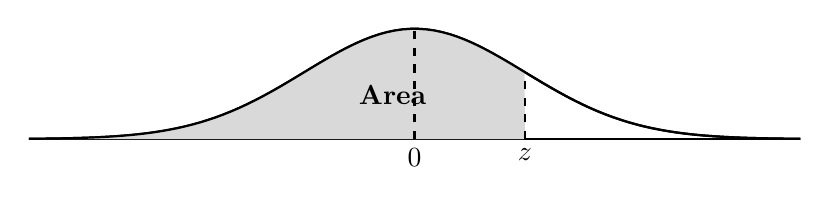
\begin{tikzpicture}[scale=1.4]
    % Draw baseline
    \draw (-3.5,0) -- (3.5,0);
    
    % Draw curve
    \draw[thick, domain=-3.5:3.5, samples=100] plot (\x, {exp(-0.5*\x*\x)});
    
    % Shaded Area from -infinity to z
    \fill[gray!30, domain=-3.5:1.0, samples=100] plot (\x, {exp(-0.5*\x*\x)}) -- (1.0,0) -- (-3.5,0) -- cycle;
    
    % Redraw curve over shading
    \draw[thick, domain=-3.5:3.5, samples=100] plot (\x, {exp(-0.5*\x*\x)});
    
    % Draw center dashed line and z line
    \draw[dashed, thick] (0,0) -- (0,1);
    \draw[dashed, thick] (1.0,0) -- (1.0,{exp(-0.5*1.0*1.0)});
    
    % Add labels
    \node[below] at (0,0) {0};
    \node[below] at (1.0,0) {$z$};
    \node at (-0.2, 0.4) {\textbf{Area}};
\end{tikzpicture}
\end{center}

\vspace{0.3cm}
\noindent\textbf{Table A.3} Areas under the Normal Curve
\vspace{0.2cm}

% ================= COMBINED CONTINUOUS TABLE =================
\begin{center}
\small
\begin{longtable}{ccccccccccc}
\toprule\toprule
$z$ & .00 & .01 & .02 & .03 & .04 & .05 & .06 & .07 & .08 & .09 \\
\midrule
\endhead % This header repeats on every new page

\midrule
\multicolumn{11}{r}{{Continued on next page}} \\
\bottomrule
\endfoot

\bottomrule\bottomrule
\endlastfoot

% --- Negative Z-Scores ---
-3.4 & 0.0003 & 0.0003 & 0.0003 & 0.0003 & 0.0003 & 0.0003 & 0.0003 & 0.0003 & 0.0003 & 0.0002 \\
-3.3 & 0.0005 & 0.0005 & 0.0005 & 0.0004 & 0.0004 & 0.0004 & 0.0004 & 0.0004 & 0.0004 & 0.0003 \\
-3.2 & 0.0007 & 0.0007 & 0.0006 & 0.0006 & 0.0006 & 0.0006 & 0.0006 & 0.0005 & 0.0005 & 0.0005 \\
-3.1 & 0.0010 & 0.0009 & 0.0009 & 0.0009 & 0.0008 & 0.0008 & 0.0008 & 0.0008 & 0.0007 & 0.0007 \\
-3.0 & 0.0013 & 0.0013 & 0.0013 & 0.0012 & 0.0012 & 0.0011 & 0.0011 & 0.0011 & 0.0010 & 0.0010 \\
\addlinespace
-2.9 & 0.0019 & 0.0018 & 0.0017 & 0.0017 & 0.0016 & 0.0016 & 0.0015 & 0.0015 & 0.0014 & 0.0014 \\
-2.8 & 0.0026 & 0.0025 & 0.0024 & 0.0023 & 0.0023 & 0.0022 & 0.0021 & 0.0021 & 0.0020 & 0.0019 \\
-2.7 & 0.0035 & 0.0034 & 0.0033 & 0.0032 & 0.0031 & 0.0030 & 0.0029 & 0.0028 & 0.0027 & 0.0026 \\
-2.6 & 0.0047 & 0.0045 & 0.0044 & 0.0043 & 0.0041 & 0.0040 & 0.0039 & 0.0038 & 0.0037 & 0.0036 \\
-2.5 & 0.0062 & 0.0060 & 0.0059 & 0.0057 & 0.0055 & 0.0054 & 0.0052 & 0.0051 & 0.0049 & 0.0048 \\
\addlinespace
-2.4 & 0.0082 & 0.0080 & 0.0078 & 0.0075 & 0.0073 & 0.0071 & 0.0069 & 0.0068 & 0.0066 & 0.0064 \\
-2.3 & 0.0107 & 0.0104 & 0.0102 & 0.0099 & 0.0096 & 0.0094 & 0.0091 & 0.0089 & 0.0087 & 0.0084 \\
-2.2 & 0.0139 & 0.0136 & 0.0132 & 0.0129 & 0.0125 & 0.0122 & 0.0119 & 0.0116 & 0.0113 & 0.0110 \\
-2.1 & 0.0179 & 0.0174 & 0.0170 & 0.0166 & 0.0162 & 0.0158 & 0.0154 & 0.0150 & 0.0146 & 0.0143 \\
-2.0 & 0.0228 & 0.0222 & 0.0217 & 0.0212 & 0.0207 & 0.0202 & 0.0197 & 0.0192 & 0.0188 & 0.0183 \\
\addlinespace
-1.9 & 0.0287 & 0.0281 & 0.0274 & 0.0268 & 0.0262 & 0.0256 & 0.0250 & 0.0244 & 0.0239 & 0.0233 \\
-1.8 & 0.0359 & 0.0352 & 0.0344 & 0.0336 & 0.0329 & 0.0322 & 0.0314 & 0.0307 & 0.0301 & 0.0294 \\
-1.7 & 0.0446 & 0.0436 & 0.0427 & 0.0418 & 0.0409 & 0.0401 & 0.0392 & 0.0384 & 0.0375 & 0.0367 \\
-1.6 & 0.0548 & 0.0537 & 0.0526 & 0.0516 & 0.0505 & 0.0495 & 0.0485 & 0.0475 & 0.0465 & 0.0455 \\
-1.5 & 0.0668 & 0.0655 & 0.0643 & 0.0630 & 0.0618 & 0.0606 & 0.0594 & 0.0582 & 0.0571 & 0.0559 \\
\addlinespace
-1.4 & 0.0808 & 0.0793 & 0.0778 & 0.0764 & 0.0749 & 0.0735 & 0.0722 & 0.0708 & 0.0694 & 0.0681 \\
-1.3 & 0.0968 & 0.0951 & 0.0934 & 0.0918 & 0.0901 & 0.0885 & 0.0869 & 0.0853 & 0.0838 & 0.0823 \\
-1.2 & 0.1151 & 0.1131 & 0.1112 & 0.1093 & 0.1075 & 0.1056 & 0.1038 & 0.1020 & 0.1003 & 0.0985 \\
-1.1 & 0.1357 & 0.1335 & 0.1314 & 0.1292 & 0.1271 & 0.1251 & 0.1230 & 0.1210 & 0.1190 & 0.1170 \\
-1.0 & 0.1587 & 0.1562 & 0.1539 & 0.1515 & 0.1492 & 0.1469 & 0.1446 & 0.1423 & 0.1401 & 0.1379 \\
\addlinespace
-0.9 & 0.1841 & 0.1814 & 0.1788 & 0.1762 & 0.1736 & 0.1711 & 0.1685 & 0.1660 & 0.1635 & 0.1611 \\
-0.8 & 0.2119 & 0.2090 & 0.2061 & 0.2033 & 0.2005 & 0.1977 & 0.1949 & 0.1922 & 0.1894 & 0.1867 \\
-0.7 & 0.2420 & 0.2389 & 0.2358 & 0.2327 & 0.2296 & 0.2266 & 0.2236 & 0.2206 & 0.2177 & 0.2148 \\
-0.6 & 0.2743 & 0.2709 & 0.2676 & 0.2643 & 0.2611 & 0.2578 & 0.2546 & 0.2514 & 0.2483 & 0.2451 \\
-0.5 & 0.3085 & 0.3050 & 0.3015 & 0.2981 & 0.2946 & 0.2912 & 0.2877 & 0.2843 & 0.2810 & 0.2776 \\
\addlinespace
-0.4 & 0.3446 & 0.3409 & 0.3372 & 0.3336 & 0.3300 & 0.3264 & 0.3228 & 0.3192 & 0.3156 & 0.3121 \\
-0.3 & 0.3821 & 0.3783 & 0.3745 & 0.3707 & 0.3669 & 0.3632 & 0.3594 & 0.3557 & 0.3520 & 0.3483 \\
-0.2 & 0.4207 & 0.4168 & 0.4129 & 0.4090 & 0.4052 & 0.4013 & 0.3974 & 0.3936 & 0.3897 & 0.3859 \\
-0.1 & 0.4602 & 0.4562 & 0.4522 & 0.4483 & 0.4443 & 0.4404 & 0.4364 & 0.4325 & 0.4286 & 0.4247 \\
-0.0 & 0.5000 & 0.4960 & 0.4920 & 0.4880 & 0.4840 & 0.4801 & 0.4761 & 0.4721 & 0.4681 & 0.4641 \\
\midrule
% --- Positive Z-Scores ---
0.0 & 0.5000 & 0.5040 & 0.5080 & 0.5120 & 0.5160 & 0.5199 & 0.5239 & 0.5279 & 0.5319 & 0.5359 \\
0.1 & 0.5398 & 0.5438 & 0.5478 & 0.5517 & 0.5557 & 0.5596 & 0.5636 & 0.5675 & 0.5714 & 0.5753 \\
0.2 & 0.5793 & 0.5832 & 0.5871 & 0.5910 & 0.5948 & 0.5987 & 0.6026 & 0.6064 & 0.6103 & 0.6141 \\
0.3 & 0.6179 & 0.6217 & 0.6255 & 0.6293 & 0.6331 & 0.6368 & 0.6406 & 0.6443 & 0.6480 & 0.6517 \\
0.4 & 0.6554 & 0.6591 & 0.6628 & 0.6664 & 0.6700 & 0.6736 & 0.6772 & 0.6808 & 0.6844 & 0.6879 \\
\addlinespace
0.5 & 0.6915 & 0.6950 & 0.6985 & 0.7019 & 0.7054 & 0.7088 & 0.7123 & 0.7157 & 0.7190 & 0.7224 \\
0.6 & 0.7257 & 0.7291 & 0.7324 & 0.7357 & 0.7389 & 0.7422 & 0.7454 & 0.7486 & 0.7517 & 0.7549 \\
0.7 & 0.7580 & 0.7611 & 0.7642 & 0.7673 & 0.7704 & 0.7734 & 0.7764 & 0.7794 & 0.7823 & 0.7852 \\
0.8 & 0.7881 & 0.7910 & 0.7939 & 0.7967 & 0.7995 & 0.8023 & 0.8051 & 0.8078 & 0.8106 & 0.8133 \\
0.9 & 0.8159 & 0.8186 & 0.8212 & 0.8238 & 0.8264 & 0.8289 & 0.8315 & 0.8340 & 0.8365 & 0.8389 \\
\addlinespace
1.0 & 0.8413 & 0.8438 & 0.8461 & 0.8485 & 0.8508 & 0.8531 & 0.8554 & 0.8577 & 0.8599 & 0.8621 \\
1.1 & 0.8643 & 0.8665 & 0.8686 & 0.8708 & 0.8729 & 0.8749 & 0.8770 & 0.8790 & 0.8810 & 0.8830 \\
1.2 & 0.8849 & 0.8869 & 0.8888 & 0.8907 & 0.8925 & 0.8944 & 0.8962 & 0.8980 & 0.8997 & 0.9015 \\
1.3 & 0.9032 & 0.9049 & 0.9066 & 0.9082 & 0.9099 & 0.9115 & 0.9131 & 0.9147 & 0.9162 & 0.9177 \\
1.4 & 0.9192 & 0.9207 & 0.9222 & 0.9236 & 0.9251 & 0.9265 & 0.9278 & 0.9292 & 0.9306 & 0.9319 \\
\addlinespace
1.5 & 0.9332 & 0.9345 & 0.9357 & 0.9370 & 0.9382 & 0.9394 & 0.9406 & 0.9418 & 0.9429 & 0.9441 \\
1.6 & 0.9452 & 0.9463 & 0.9474 & 0.9484 & 0.9495 & 0.9505 & 0.9515 & 0.9525 & 0.9535 & 0.9545 \\
1.7 & 0.9554 & 0.9564 & 0.9573 & 0.9582 & 0.9591 & 0.9599 & 0.9608 & 0.9616 & 0.9625 & 0.9633 \\
1.8 & 0.9641 & 0.9649 & 0.9656 & 0.9664 & 0.9671 & 0.9678 & 0.9686 & 0.9693 & 0.9699 & 0.9706 \\
1.9 & 0.9713 & 0.9719 & 0.9726 & 0.9732 & 0.9738 & 0.9744 & 0.9750 & 0.9756 & 0.9761 & 0.9767 \\
\addlinespace
2.0 & 0.9772 & 0.9778 & 0.9783 & 0.9788 & 0.9793 & 0.9798 & 0.9803 & 0.9808 & 0.9812 & 0.9817 \\
2.1 & 0.9821 & 0.9826 & 0.9830 & 0.9834 & 0.9838 & 0.9842 & 0.9846 & 0.9850 & 0.9854 & 0.9857 \\
2.2 & 0.9861 & 0.9864 & 0.9868 & 0.9871 & 0.9875 & 0.9878 & 0.9881 & 0.9884 & 0.9887 & 0.9890 \\
2.3 & 0.9893 & 0.9896 & 0.9898 & 0.9901 & 0.9904 & 0.9906 & 0.9909 & 0.9911 & 0.9913 & 0.9916 \\
2.4 & 0.9918 & 0.9920 & 0.9922 & 0.9925 & 0.9927 & 0.9929 & 0.9931 & 0.9932 & 0.9934 & 0.9936 \\
\addlinespace
2.5 & 0.9938 & 0.9940 & 0.9941 & 0.9943 & 0.9945 & 0.9946 & 0.9948 & 0.9949 & 0.9951 & 0.9952 \\
2.6 & 0.9953 & 0.9955 & 0.9956 & 0.9957 & 0.9959 & 0.9960 & 0.9961 & 0.9962 & 0.9963 & 0.9964 \\
2.7 & 0.9965 & 0.9966 & 0.9967 & 0.9968 & 0.9969 & 0.9970 & 0.9971 & 0.9972 & 0.9973 & 0.9974 \\
2.8 & 0.9974 & 0.9975 & 0.9976 & 0.9977 & 0.9977 & 0.9978 & 0.9979 & 0.9979 & 0.9980 & 0.9981 \\
2.9 & 0.9981 & 0.9982 & 0.9982 & 0.9983 & 0.9984 & 0.9984 & 0.9985 & 0.9985 & 0.9986 & 0.9986 \\
\addlinespace
3.0 & 0.9987 & 0.9987 & 0.9987 & 0.9987 & 0.9988 & 0.9988 & 0.9989 & 0.9989 & 0.9990 & 0.9990 \\
3.1 & 0.9990 & 0.9991 & 0.9991 & 0.9991 & 0.9992 & 0.9992 & 0.9992 & 0.9992 & 0.9993 & 0.9993 \\
3.2 & 0.9993 & 0.9993 & 0.9994 & 0.9994 & 0.9994 & 0.9994 & 0.9994 & 0.9995 & 0.9995 & 0.9995 \\
3.3 & 0.9995 & 0.9995 & 0.9995 & 0.9996 & 0.9996 & 0.9996 & 0.9996 & 0.9996 & 0.9996 & 0.9997 \\
3.4 & 0.9997 & 0.9997 & 0.9997 & 0.9997 & 0.9997 & 0.9997 & 0.9997 & 0.9997 & 0.9997 & 0.9998 \\
\end{longtable}
\end{center}


\mk{18} \yr{MATH 245 | L-2/T-1 | 2020--21}

\item In a manufacturing process, bubbles occur in glass products, on average 1 in every 1000 items produced. What is the probability that a random sample of 8000 will yield fewer than 7 items with bubbles?
\mk{10} \yr{MATH 245 | L-2/T-1 | 2019--20}

\item The time between emergency calls to a fire station follows an exponential distribution with an average rate of 1.8 calls per day. (i) What is the chance of a call in the next 15 minutes? (ii) What if there has been no call for the entire shift so far? (iii) What is the probability of no calls during a 10-hour shift? (iv) No calls in four successive days? (v) In 10\% of shifts, there's a call in the first $x$ hours; find $x$.
\mk{25} \yr{MATH 245 | L-2/T-1 | 2019--20}

\item A continuous random variable $X$ has density $f(x)=e^{-x}$ for $x>0$ (and 0 otherwise). Find the expected value of $g(X)=e^{2X/3}$.
\mk{18} \yr{MATH 245 | L-2/T-1 | 2019--20}

\item The marks in a test are normally distributed. It is known that 10\% of students have marks under 65 and 25\% exceed 75. What percentage have marks between 60 and 74?

% ================= DIAGRAM =================
\begin{center}
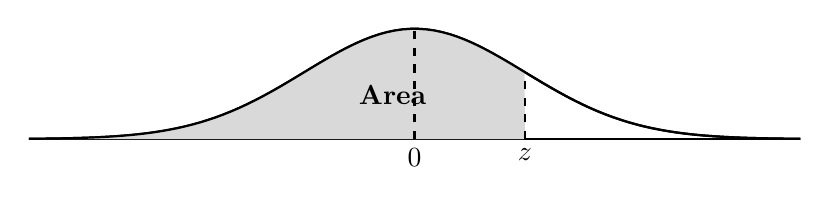
\begin{tikzpicture}[scale=1.4]
    % Draw baseline
    \draw (-3.5,0) -- (3.5,0);
    
    % Draw curve
    \draw[thick, domain=-3.5:3.5, samples=100] plot (\x, {exp(-0.5*\x*\x)});
    
    % Shaded Area from -infinity to z
    \fill[gray!30, domain=-3.5:1.0, samples=100] plot (\x, {exp(-0.5*\x*\x)}) -- (1.0,0) -- (-3.5,0) -- cycle;
    
    % Redraw curve over shading
    \draw[thick, domain=-3.5:3.5, samples=100] plot (\x, {exp(-0.5*\x*\x)});
    
    % Draw center dashed line and z line
    \draw[dashed, thick] (0,0) -- (0,1);
    \draw[dashed, thick] (1.0,0) -- (1.0,{exp(-0.5*1.0*1.0)});
    
    % Add labels
    \node[below] at (0,0) {0};
    \node[below] at (1.0,0) {$z$};
    \node at (-0.2, 0.4) {\textbf{Area}};
\end{tikzpicture}
\end{center}

\vspace{0.3cm}
\noindent\textbf{Table A.3} Areas under the Normal Curve
\vspace{0.2cm}

% ================= COMBINED CONTINUOUS TABLE =================
\begin{center}
\small
\begin{longtable}{ccccccccccc}
\toprule\toprule
$z$ & .00 & .01 & .02 & .03 & .04 & .05 & .06 & .07 & .08 & .09 \\
\midrule
\endhead % This header repeats on every new page

\midrule
\multicolumn{11}{r}{{Continued on next page}} \\
\bottomrule
\endfoot

\bottomrule\bottomrule
\endlastfoot

% --- Negative Z-Scores ---
-3.4 & 0.0003 & 0.0003 & 0.0003 & 0.0003 & 0.0003 & 0.0003 & 0.0003 & 0.0003 & 0.0003 & 0.0002 \\
-3.3 & 0.0005 & 0.0005 & 0.0005 & 0.0004 & 0.0004 & 0.0004 & 0.0004 & 0.0004 & 0.0004 & 0.0003 \\
-3.2 & 0.0007 & 0.0007 & 0.0006 & 0.0006 & 0.0006 & 0.0006 & 0.0006 & 0.0005 & 0.0005 & 0.0005 \\
-3.1 & 0.0010 & 0.0009 & 0.0009 & 0.0009 & 0.0008 & 0.0008 & 0.0008 & 0.0008 & 0.0007 & 0.0007 \\
-3.0 & 0.0013 & 0.0013 & 0.0013 & 0.0012 & 0.0012 & 0.0011 & 0.0011 & 0.0011 & 0.0010 & 0.0010 \\
\addlinespace
-2.9 & 0.0019 & 0.0018 & 0.0017 & 0.0017 & 0.0016 & 0.0016 & 0.0015 & 0.0015 & 0.0014 & 0.0014 \\
-2.8 & 0.0026 & 0.0025 & 0.0024 & 0.0023 & 0.0023 & 0.0022 & 0.0021 & 0.0021 & 0.0020 & 0.0019 \\
-2.7 & 0.0035 & 0.0034 & 0.0033 & 0.0032 & 0.0031 & 0.0030 & 0.0029 & 0.0028 & 0.0027 & 0.0026 \\
-2.6 & 0.0047 & 0.0045 & 0.0044 & 0.0043 & 0.0041 & 0.0040 & 0.0039 & 0.0038 & 0.0037 & 0.0036 \\
-2.5 & 0.0062 & 0.0060 & 0.0059 & 0.0057 & 0.0055 & 0.0054 & 0.0052 & 0.0051 & 0.0049 & 0.0048 \\
\addlinespace
-2.4 & 0.0082 & 0.0080 & 0.0078 & 0.0075 & 0.0073 & 0.0071 & 0.0069 & 0.0068 & 0.0066 & 0.0064 \\
-2.3 & 0.0107 & 0.0104 & 0.0102 & 0.0099 & 0.0096 & 0.0094 & 0.0091 & 0.0089 & 0.0087 & 0.0084 \\
-2.2 & 0.0139 & 0.0136 & 0.0132 & 0.0129 & 0.0125 & 0.0122 & 0.0119 & 0.0116 & 0.0113 & 0.0110 \\
-2.1 & 0.0179 & 0.0174 & 0.0170 & 0.0166 & 0.0162 & 0.0158 & 0.0154 & 0.0150 & 0.0146 & 0.0143 \\
-2.0 & 0.0228 & 0.0222 & 0.0217 & 0.0212 & 0.0207 & 0.0202 & 0.0197 & 0.0192 & 0.0188 & 0.0183 \\
\addlinespace
-1.9 & 0.0287 & 0.0281 & 0.0274 & 0.0268 & 0.0262 & 0.0256 & 0.0250 & 0.0244 & 0.0239 & 0.0233 \\
-1.8 & 0.0359 & 0.0352 & 0.0344 & 0.0336 & 0.0329 & 0.0322 & 0.0314 & 0.0307 & 0.0301 & 0.0294 \\
-1.7 & 0.0446 & 0.0436 & 0.0427 & 0.0418 & 0.0409 & 0.0401 & 0.0392 & 0.0384 & 0.0375 & 0.0367 \\
-1.6 & 0.0548 & 0.0537 & 0.0526 & 0.0516 & 0.0505 & 0.0495 & 0.0485 & 0.0475 & 0.0465 & 0.0455 \\
-1.5 & 0.0668 & 0.0655 & 0.0643 & 0.0630 & 0.0618 & 0.0606 & 0.0594 & 0.0582 & 0.0571 & 0.0559 \\
\addlinespace
-1.4 & 0.0808 & 0.0793 & 0.0778 & 0.0764 & 0.0749 & 0.0735 & 0.0722 & 0.0708 & 0.0694 & 0.0681 \\
-1.3 & 0.0968 & 0.0951 & 0.0934 & 0.0918 & 0.0901 & 0.0885 & 0.0869 & 0.0853 & 0.0838 & 0.0823 \\
-1.2 & 0.1151 & 0.1131 & 0.1112 & 0.1093 & 0.1075 & 0.1056 & 0.1038 & 0.1020 & 0.1003 & 0.0985 \\
-1.1 & 0.1357 & 0.1335 & 0.1314 & 0.1292 & 0.1271 & 0.1251 & 0.1230 & 0.1210 & 0.1190 & 0.1170 \\
-1.0 & 0.1587 & 0.1562 & 0.1539 & 0.1515 & 0.1492 & 0.1469 & 0.1446 & 0.1423 & 0.1401 & 0.1379 \\
\addlinespace
-0.9 & 0.1841 & 0.1814 & 0.1788 & 0.1762 & 0.1736 & 0.1711 & 0.1685 & 0.1660 & 0.1635 & 0.1611 \\
-0.8 & 0.2119 & 0.2090 & 0.2061 & 0.2033 & 0.2005 & 0.1977 & 0.1949 & 0.1922 & 0.1894 & 0.1867 \\
-0.7 & 0.2420 & 0.2389 & 0.2358 & 0.2327 & 0.2296 & 0.2266 & 0.2236 & 0.2206 & 0.2177 & 0.2148 \\
-0.6 & 0.2743 & 0.2709 & 0.2676 & 0.2643 & 0.2611 & 0.2578 & 0.2546 & 0.2514 & 0.2483 & 0.2451 \\
-0.5 & 0.3085 & 0.3050 & 0.3015 & 0.2981 & 0.2946 & 0.2912 & 0.2877 & 0.2843 & 0.2810 & 0.2776 \\
\addlinespace
-0.4 & 0.3446 & 0.3409 & 0.3372 & 0.3336 & 0.3300 & 0.3264 & 0.3228 & 0.3192 & 0.3156 & 0.3121 \\
-0.3 & 0.3821 & 0.3783 & 0.3745 & 0.3707 & 0.3669 & 0.3632 & 0.3594 & 0.3557 & 0.3520 & 0.3483 \\
-0.2 & 0.4207 & 0.4168 & 0.4129 & 0.4090 & 0.4052 & 0.4013 & 0.3974 & 0.3936 & 0.3897 & 0.3859 \\
-0.1 & 0.4602 & 0.4562 & 0.4522 & 0.4483 & 0.4443 & 0.4404 & 0.4364 & 0.4325 & 0.4286 & 0.4247 \\
-0.0 & 0.5000 & 0.4960 & 0.4920 & 0.4880 & 0.4840 & 0.4801 & 0.4761 & 0.4721 & 0.4681 & 0.4641 \\
\midrule
% --- Positive Z-Scores ---
0.0 & 0.5000 & 0.5040 & 0.5080 & 0.5120 & 0.5160 & 0.5199 & 0.5239 & 0.5279 & 0.5319 & 0.5359 \\
0.1 & 0.5398 & 0.5438 & 0.5478 & 0.5517 & 0.5557 & 0.5596 & 0.5636 & 0.5675 & 0.5714 & 0.5753 \\
0.2 & 0.5793 & 0.5832 & 0.5871 & 0.5910 & 0.5948 & 0.5987 & 0.6026 & 0.6064 & 0.6103 & 0.6141 \\
0.3 & 0.6179 & 0.6217 & 0.6255 & 0.6293 & 0.6331 & 0.6368 & 0.6406 & 0.6443 & 0.6480 & 0.6517 \\
0.4 & 0.6554 & 0.6591 & 0.6628 & 0.6664 & 0.6700 & 0.6736 & 0.6772 & 0.6808 & 0.6844 & 0.6879 \\
\addlinespace
0.5 & 0.6915 & 0.6950 & 0.6985 & 0.7019 & 0.7054 & 0.7088 & 0.7123 & 0.7157 & 0.7190 & 0.7224 \\
0.6 & 0.7257 & 0.7291 & 0.7324 & 0.7357 & 0.7389 & 0.7422 & 0.7454 & 0.7486 & 0.7517 & 0.7549 \\
0.7 & 0.7580 & 0.7611 & 0.7642 & 0.7673 & 0.7704 & 0.7734 & 0.7764 & 0.7794 & 0.7823 & 0.7852 \\
0.8 & 0.7881 & 0.7910 & 0.7939 & 0.7967 & 0.7995 & 0.8023 & 0.8051 & 0.8078 & 0.8106 & 0.8133 \\
0.9 & 0.8159 & 0.8186 & 0.8212 & 0.8238 & 0.8264 & 0.8289 & 0.8315 & 0.8340 & 0.8365 & 0.8389 \\
\addlinespace
1.0 & 0.8413 & 0.8438 & 0.8461 & 0.8485 & 0.8508 & 0.8531 & 0.8554 & 0.8577 & 0.8599 & 0.8621 \\
1.1 & 0.8643 & 0.8665 & 0.8686 & 0.8708 & 0.8729 & 0.8749 & 0.8770 & 0.8790 & 0.8810 & 0.8830 \\
1.2 & 0.8849 & 0.8869 & 0.8888 & 0.8907 & 0.8925 & 0.8944 & 0.8962 & 0.8980 & 0.8997 & 0.9015 \\
1.3 & 0.9032 & 0.9049 & 0.9066 & 0.9082 & 0.9099 & 0.9115 & 0.9131 & 0.9147 & 0.9162 & 0.9177 \\
1.4 & 0.9192 & 0.9207 & 0.9222 & 0.9236 & 0.9251 & 0.9265 & 0.9278 & 0.9292 & 0.9306 & 0.9319 \\
\addlinespace
1.5 & 0.9332 & 0.9345 & 0.9357 & 0.9370 & 0.9382 & 0.9394 & 0.9406 & 0.9418 & 0.9429 & 0.9441 \\
1.6 & 0.9452 & 0.9463 & 0.9474 & 0.9484 & 0.9495 & 0.9505 & 0.9515 & 0.9525 & 0.9535 & 0.9545 \\
1.7 & 0.9554 & 0.9564 & 0.9573 & 0.9582 & 0.9591 & 0.9599 & 0.9608 & 0.9616 & 0.9625 & 0.9633 \\
1.8 & 0.9641 & 0.9649 & 0.9656 & 0.9664 & 0.9671 & 0.9678 & 0.9686 & 0.9693 & 0.9699 & 0.9706 \\
1.9 & 0.9713 & 0.9719 & 0.9726 & 0.9732 & 0.9738 & 0.9744 & 0.9750 & 0.9756 & 0.9761 & 0.9767 \\
\addlinespace
2.0 & 0.9772 & 0.9778 & 0.9783 & 0.9788 & 0.9793 & 0.9798 & 0.9803 & 0.9808 & 0.9812 & 0.9817 \\
2.1 & 0.9821 & 0.9826 & 0.9830 & 0.9834 & 0.9838 & 0.9842 & 0.9846 & 0.9850 & 0.9854 & 0.9857 \\
2.2 & 0.9861 & 0.9864 & 0.9868 & 0.9871 & 0.9875 & 0.9878 & 0.9881 & 0.9884 & 0.9887 & 0.9890 \\
2.3 & 0.9893 & 0.9896 & 0.9898 & 0.9901 & 0.9904 & 0.9906 & 0.9909 & 0.9911 & 0.9913 & 0.9916 \\
2.4 & 0.9918 & 0.9920 & 0.9922 & 0.9925 & 0.9927 & 0.9929 & 0.9931 & 0.9932 & 0.9934 & 0.9936 \\
\addlinespace
2.5 & 0.9938 & 0.9940 & 0.9941 & 0.9943 & 0.9945 & 0.9946 & 0.9948 & 0.9949 & 0.9951 & 0.9952 \\
2.6 & 0.9953 & 0.9955 & 0.9956 & 0.9957 & 0.9959 & 0.9960 & 0.9961 & 0.9962 & 0.9963 & 0.9964 \\
2.7 & 0.9965 & 0.9966 & 0.9967 & 0.9968 & 0.9969 & 0.9970 & 0.9971 & 0.9972 & 0.9973 & 0.9974 \\
2.8 & 0.9974 & 0.9975 & 0.9976 & 0.9977 & 0.9977 & 0.9978 & 0.9979 & 0.9979 & 0.9980 & 0.9981 \\
2.9 & 0.9981 & 0.9982 & 0.9982 & 0.9983 & 0.9984 & 0.9984 & 0.9985 & 0.9985 & 0.9986 & 0.9986 \\
\addlinespace
3.0 & 0.9987 & 0.9987 & 0.9987 & 0.9987 & 0.9988 & 0.9988 & 0.9989 & 0.9989 & 0.9990 & 0.9990 \\
3.1 & 0.9990 & 0.9991 & 0.9991 & 0.9991 & 0.9992 & 0.9992 & 0.9992 & 0.9992 & 0.9993 & 0.9993 \\
3.2 & 0.9993 & 0.9993 & 0.9994 & 0.9994 & 0.9994 & 0.9994 & 0.9994 & 0.9995 & 0.9995 & 0.9995 \\
3.3 & 0.9995 & 0.9995 & 0.9995 & 0.9996 & 0.9996 & 0.9996 & 0.9996 & 0.9996 & 0.9996 & 0.9997 \\
3.4 & 0.9997 & 0.9997 & 0.9997 & 0.9997 & 0.9997 & 0.9997 & 0.9997 & 0.9997 & 0.9997 & 0.9998 \\
\end{longtable}
\end{center}

\mk{12} \yr{MATH 241 | L-2/T-1 | 2015--16}

\end{enumerate}


\section{S9. Statistical Inference}
\label{sec:S9}
\markboth{S9. Statistical Inference}{}

%%──────────────────────────────────────────────────────────────────────
\subtopic{cG}{Sampling Distributions \& Central Limit Theorem}
\label{sub:s9-sampling}

\begin{enumerate}\item The masses of 1500 ball bearings are normally distributed with a mean of 22.40 g and a standard deviation of 0.048 g. If 300 random samples of size 36 are drawn, determine the expected mean and standard deviation of the sampling distribution of means (with and without replacement). How many of the random samples would have their means:
\begin{enumerate}
  \item between 22.39 and 22.41 g?
  \item greater than 22.42 g?
  \item less than 22.38 g or more than 22.41 g?
\end{enumerate}

% ================= NORMAL DISTRIBUTION DIAGRAM =================
\begin{center}
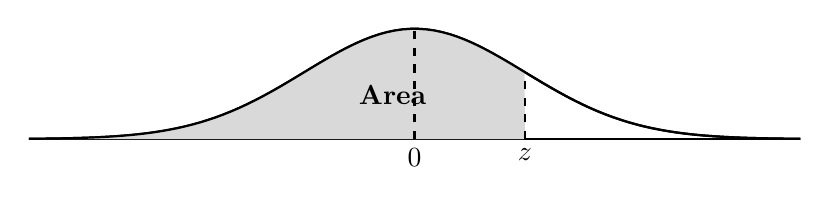
\begin{tikzpicture}[scale=1.4]
    % Draw baseline
    \draw (-3.5,0) -- (3.5,0);
    
    % Draw curve
    \draw[thick, domain=-3.5:3.5, samples=100] plot (\x, {exp(-0.5*\x*\x)});
    
    % Shaded Area from -infinity to z (positive z side)
    \fill[gray!30, domain=-3.5:1.0, samples=100] plot (\x, {exp(-0.5*\x*\x)}) -- (1.0,0) -- (-3.5,0) -- cycle;
    
    % Redraw curve over shading to keep the line crisp
    \draw[thick, domain=-3.5:3.5, samples=100] plot (\x, {exp(-0.5*\x*\x)});
    
    % Draw center dashed line and z line
    \draw[dashed, thick] (0,0) -- (0,1);
    \draw[dashed, thick] (1.0,0) -- (1.0,{exp(-0.5*1.0*1.0)});
    
    % Add labels
    \node[below] at (0,0) {0};
    \node[below] at (1.0,0) {$z$};
    \node at (-0.2, 0.4) {\textbf{Area}};
\end{tikzpicture}
\end{center}

\vspace{0.3cm}
\noindent\textbf{Table A.3 (continued)} Areas under the Normal Curve
\vspace{0.2cm}

% ================= DATA TABLE =================
\begin{center}
\small
\begin{longtable}{ccccccccccc}
\toprule\toprule
$z$ & .00 & .01 & .02 & .03 & .04 & .05 & .06 & .07 & .08 & .09 \\
\midrule
\endhead
\bottomrule\bottomrule
\endfoot
0.0 & 0.5000 & 0.5040 & 0.5080 & 0.5120 & 0.5160 & 0.5199 & 0.5239 & 0.5279 & 0.5319 & 0.5359 \\
0.1 & 0.5398 & 0.5438 & 0.5478 & 0.5517 & 0.5557 & 0.5596 & 0.5636 & 0.5675 & 0.5714 & 0.5753 \\
0.2 & 0.5793 & 0.5832 & 0.5871 & 0.5910 & 0.5948 & 0.5987 & 0.6026 & 0.6064 & 0.6103 & 0.6141 \\
0.3 & 0.6179 & 0.6217 & 0.6255 & 0.6293 & 0.6331 & 0.6368 & 0.6406 & 0.6443 & 0.6480 & 0.6517 \\
0.4 & 0.6554 & 0.6591 & 0.6628 & 0.6664 & 0.6700 & 0.6736 & 0.6772 & 0.6808 & 0.6844 & 0.6879 \\
0.5 & 0.6915 & 0.6950 & 0.6985 & 0.7019 & 0.7054 & 0.7088 & 0.7123 & 0.7157 & 0.7190 & 0.7224 \\
0.6 & 0.7257 & 0.7291 & 0.7324 & 0.7357 & 0.7389 & 0.7422 & 0.7454 & 0.7486 & 0.7517 & 0.7549 \\
0.7 & 0.7580 & 0.7611 & 0.7642 & 0.7673 & 0.7704 & 0.7734 & 0.7764 & 0.7794 & 0.7823 & 0.7852 \\
0.8 & 0.7881 & 0.7910 & 0.7939 & 0.7967 & 0.7995 & 0.8023 & 0.8051 & 0.8078 & 0.8106 & 0.8133 \\
0.9 & 0.8159 & 0.8186 & 0.8212 & 0.8238 & 0.8264 & 0.8289 & 0.8315 & 0.8340 & 0.8365 & 0.8389 \\
1.0 & 0.8413 & 0.8438 & 0.8461 & 0.8485 & 0.8508 & 0.8531 & 0.8554 & 0.8577 & 0.8599 & 0.8621 \\
1.1 & 0.8643 & 0.8665 & 0.8686 & 0.8708 & 0.8729 & 0.8749 & 0.8770 & 0.8790 & 0.8810 & 0.8830 \\
1.2 & 0.8849 & 0.8869 & 0.8888 & 0.8907 & 0.8925 & 0.8944 & 0.8962 & 0.8980 & 0.8997 & 0.9015 \\
1.3 & 0.9032 & 0.9049 & 0.9066 & 0.9082 & 0.9099 & 0.9115 & 0.9131 & 0.9147 & 0.9162 & 0.9177 \\
1.4 & 0.9192 & 0.9207 & 0.9222 & 0.9236 & 0.9251 & 0.9265 & 0.9278 & 0.9292 & 0.9306 & 0.9319 \\
1.5 & 0.9332 & 0.9345 & 0.9357 & 0.9370 & 0.9382 & 0.9394 & 0.9406 & 0.9418 & 0.9429 & 0.9441 \\
1.6 & 0.9452 & 0.9463 & 0.9474 & 0.9484 & 0.9495 & 0.9505 & 0.9515 & 0.9525 & 0.9535 & 0.9545 \\
1.7 & 0.9554 & 0.9564 & 0.9573 & 0.9582 & 0.9591 & 0.9599 & 0.9608 & 0.9616 & 0.9625 & 0.9633 \\
1.8 & 0.9641 & 0.9649 & 0.9656 & 0.9664 & 0.9671 & 0.9678 & 0.9686 & 0.9693 & 0.9699 & 0.9706 \\
1.9 & 0.9713 & 0.9719 & 0.9726 & 0.9732 & 0.9738 & 0.9744 & 0.9750 & 0.9756 & 0.9761 & 0.9767 \\
2.0 & 0.9772 & 0.9778 & 0.9783 & 0.9788 & 0.9793 & 0.9798 & 0.9803 & 0.9808 & 0.9812 & 0.9817 \\
2.1 & 0.9821 & 0.9826 & 0.9830 & 0.9834 & 0.9838 & 0.9842 & 0.9846 & 0.9850 & 0.9854 & 0.9857 \\
2.2 & 0.9861 & 0.9864 & 0.9868 & 0.9871 & 0.9875 & 0.9878 & 0.9881 & 0.9884 & 0.9887 & 0.9890 \\
2.3 & 0.9893 & 0.9896 & 0.9898 & 0.9901 & 0.9904 & 0.9906 & 0.9909 & 0.9911 & 0.9913 & 0.9916 \\
2.4 & 0.9918 & 0.9920 & 0.9922 & 0.9925 & 0.9927 & 0.9929 & 0.9931 & 0.9932 & 0.9934 & 0.9936 \\
2.5 & 0.9938 & 0.9940 & 0.9941 & 0.9943 & 0.9945 & 0.9946 & 0.9948 & 0.9949 & 0.9951 & 0.9952 \\
2.6 & 0.9953 & 0.9955 & 0.9956 & 0.9957 & 0.9959 & 0.9960 & 0.9961 & 0.9962 & 0.9963 & 0.9964 \\
2.7 & 0.9965 & 0.9966 & 0.9967 & 0.9968 & 0.9969 & 0.9970 & 0.9971 & 0.9972 & 0.9973 & 0.9974 \\
2.8 & 0.9974 & 0.9975 & 0.9976 & 0.9977 & 0.9977 & 0.9978 & 0.9979 & 0.9979 & 0.9980 & 0.9981 \\
2.9 & 0.9981 & 0.9982 & 0.9982 & 0.9983 & 0.9984 & 0.9984 & 0.9985 & 0.9985 & 0.9986 & 0.9986 \\
3.0 & 0.9987 & 0.9987 & 0.9987 & 0.9987 & 0.9988 & 0.9988 & 0.9989 & 0.9989 & 0.9990 & 0.9990 \\
3.1 & 0.9990 & 0.9991 & 0.9991 & 0.9991 & 0.9992 & 0.9992 & 0.9992 & 0.9992 & 0.9993 & 0.9993 \\
3.2 & 0.9993 & 0.9993 & 0.9994 & 0.9994 & 0.9994 & 0.9994 & 0.9994 & 0.9995 & 0.9995 & 0.9995 \\
3.3 & 0.9995 & 0.9995 & 0.9995 & 0.9996 & 0.9996 & 0.9996 & 0.9996 & 0.9996 & 0.9996 & 0.9997 \\
3.4 & 0.9997 & 0.9997 & 0.9997 & 0.9997 & 0.9997 & 0.9997 & 0.9997 & 0.9997 & 0.9997 & 0.9998 \\
\end{longtable}
\end{center}

\mk{15} \yr{MATH 245 | L-2/T-1 | 2016--17}

\end{enumerate}

%%──────────────────────────────────────────────────────────────────────
\subtopic{cG}{Parameter Estimation \& Confidence Intervals}
\label{sub:s9-estimation}

\begin{enumerate}\item Hello \end{enumerate}

%%──────────────────────────────────────────────────────────────────────
\subtopic{cG}{Tests of Hypothesis}
\label{sub:s9-hypothesis}

\begin{enumerate}\item Ten individuals were chosen at random and their heights (inches) found to be 63, 63, 64, 65, 66, 69, 69, 70, 70, 71. Discuss whether the mean height of the universe is 65 inches. ($t_{9}=2.262$ at 5\% significance.)
\mk{17} \yr{MATH 245 | L-2/T-1 | 2021--22}

\item According to a dietary study, high sodium intake may be related to ulcers, stomach cancer, and migraine headaches. The human requirement for salt is only 220 milligrams per day. A random sample of 20 similar servings of a certain cereal has a mean sodium content of 244 milligrams and a standard deviation of 24.5 milligrams. Does this suggest, at the 0.05 level of significance, that the average sodium content is greater than 220 milligrams?

% ================= STUDENT'S T DISTRIBUTION =================
\begin{center}
\begin{minipage}{0.45\textwidth}
    \centering
    \textbf{\large Table of the} \\
    \vspace{0.2cm}
    \textbf{\large Student's $t$-distribution} \\
    \vspace{0.4cm}
    The table gives the values of $t_{\alpha, \nu}$ where \\
    $\Pr(T_\nu > t_{\alpha, \nu}) = \alpha$, \\
    with $\nu$ degrees of freedom.
\end{minipage}
\hfill
\begin{minipage}{0.45\textwidth}
    \centering
    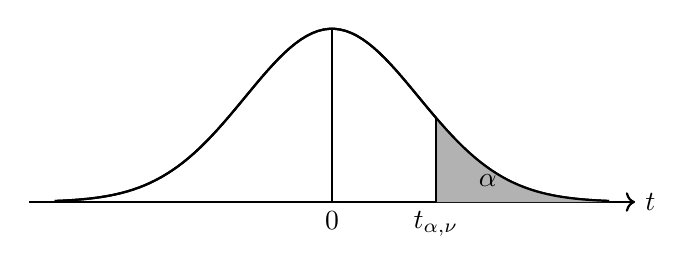
\begin{tikzpicture}[scale=1.1]
        % Draw baseline
        \draw[->, thick] (-3.5,0) -- (3.5,0) node[right] {$t$};
        
        % Draw curve
        \draw[thick, domain=-3.2:3.2, samples=100] plot (\x, {2.0*exp(-0.5*\x*\x)});
        
        % Shaded Area (right tail for alpha)
        \fill[gray!60, domain=1.2:3.2, samples=100] plot (\x, {2.0*exp(-0.5*\x*\x)}) -- (3.2,0) -- (1.2,0) -- cycle;
        
        % Redraw curve over shading
        \draw[thick, domain=-3.2:3.2, samples=100] plot (\x, {2.0*exp(-0.5*\x*\x)});
        
        % Draw center line and t_alpha line
        \draw[thick] (0,0) -- (0,2.0);
        \draw[thick] (1.2,0) -- (1.2,{2.0*exp(-0.5*1.2*1.2)});
        
        % Add labels
        \node[below] at (0,0) {0};
        \node[below] at (1.2,0) {$t_{\alpha, \nu}$};
        \node at (1.8, 0.25) {$\alpha$};
    \end{tikzpicture}
\end{minipage}
\end{center}
\vspace{0.5cm}

\begin{center}
\renewcommand{\arraystretch}{1.2}
\begin{longtable}{c | ccccccc}
\toprule
$\nu$ & $\alpha=0.1$ & $0.05$ & $0.025$ & $0.01$ & $0.005$ & $0.001$ & $0.0005$ \\
\midrule
\endfirsthead

\toprule
$\nu$ & $\alpha=0.1$ & $0.05$ & $0.025$ & $0.01$ & $0.005$ & $0.001$ & $0.0005$ \\
\midrule
\endhead

\midrule
\multicolumn{8}{r}{{Continued on next page}} \\
\bottomrule
\endfoot

\bottomrule
\endlastfoot
1 & 3.078 & 6.314 & 12.706 & 31.821 & 63.657 & 318.309 & 636.619 \\
2 & 1.886 & 2.920 & 4.303 & 6.965 & 9.925 & 22.327 & 31.599 \\
3 & 1.638 & 2.353 & 3.182 & 4.541 & 5.841 & 10.215 & 12.924 \\
4 & 1.533 & 2.132 & 2.776 & 3.747 & 4.604 & 7.173 & 8.610 \\
5 & 1.476 & 2.015 & 2.571 & 3.365 & 4.032 & 5.893 & 6.869 \\
6 & 1.440 & 1.943 & 2.447 & 3.143 & 3.707 & 5.208 & 5.959 \\
7 & 1.415 & 1.895 & 2.365 & 2.998 & 3.499 & 4.785 & 5.408 \\
8 & 1.397 & 1.860 & 2.306 & 2.896 & 3.355 & 4.501 & 5.041 \\
9 & 1.383 & 1.833 & 2.262 & 2.821 & 3.250 & 4.297 & 4.781 \\
10 & 1.372 & 1.812 & 2.228 & 2.764 & 3.169 & 4.144 & 4.587 \\
11 & 1.363 & 1.796 & 2.201 & 2.718 & 3.106 & 4.025 & 4.437 \\
12 & 1.356 & 1.782 & 2.179 & 2.681 & 3.055 & 3.930 & 4.318 \\
13 & 1.350 & 1.771 & 2.160 & 2.650 & 3.012 & 3.852 & 4.221 \\
14 & 1.345 & 1.761 & 2.145 & 2.624 & 2.977 & 3.787 & 4.140 \\
15 & 1.341 & 1.753 & 2.131 & 2.602 & 2.947 & 3.733 & 4.073 \\
16 & 1.337 & 1.746 & 2.120 & 2.583 & 2.921 & 3.686 & 4.015 \\
17 & 1.333 & 1.740 & 2.110 & 2.567 & 2.898 & 3.646 & 3.965 \\
18 & 1.330 & 1.734 & 2.101 & 2.552 & 2.878 & 3.610 & 3.922 \\
19 & 1.328 & 1.729 & 2.093 & 2.539 & 2.861 & 3.579 & 3.883 \\
20 & 1.325 & 1.725 & 2.086 & 2.528 & 2.845 & 3.552 & 3.850 \\
21 & 1.323 & 1.721 & 2.080 & 2.518 & 2.831 & 3.527 & 3.819 \\
22 & 1.321 & 1.717 & 2.074 & 2.508 & 2.819 & 3.505 & 3.792 \\
23 & 1.319 & 1.714 & 2.069 & 2.500 & 2.807 & 3.485 & 3.768 \\
24 & 1.318 & 1.711 & 2.064 & 2.492 & 2.797 & 3.467 & 3.745 \\
25 & 1.316 & 1.708 & 2.060 & 2.485 & 2.787 & 3.450 & 3.725 \\
26 & 1.315 & 1.706 & 2.056 & 2.479 & 2.779 & 3.435 & 3.707 \\
27 & 1.314 & 1.703 & 2.052 & 2.473 & 2.771 & 3.421 & 3.690 \\
28 & 1.313 & 1.701 & 2.048 & 2.467 & 2.763 & 3.408 & 3.674 \\
29 & 1.311 & 1.699 & 2.045 & 2.462 & 2.756 & 3.396 & 3.659 \\
30 & 1.310 & 1.697 & 2.042 & 2.457 & 2.750 & 3.385 & 3.646 \\
40 & 1.303 & 1.684 & 2.021 & 2.423 & 2.704 & 3.307 & 3.551 \\
60 & 1.296 & 1.671 & 2.000 & 2.390 & 2.660 & 3.232 & 3.460 \\
120 & 1.289 & 1.658 & 1.980 & 2.358 & 2.617 & 3.160 & 3.373 \\
$\infty$ & 1.282 & 1.645 & 1.960 & 2.326 & 2.576 & 3.090 & 3.291 \\
\end{longtable}
\end{center}

\mk{15} \yr{MATH 245 | L-2/T-1 | 2020--21}

\item In a scientific paper, DNA paternity testing reliability is described as: the test is 100\% accurate if the man is not the father and 99.9\% accurate if he is. Consider the hypotheses:
\[
H_{0}: \text{a particular man is the father}, \qquad H_{a}: \text{a particular man is not the father.}
\]
Describe Type I and Type II errors in this context.
\mk{10} \yr{MATH 245 | L-2/T-1 | 2020--21}

\item In a research report, a student of Medical College claims that mice with an average life span of 32 months will live to be about 40 months old when 40\% of the calories in their diet are replaced by vitamins and protein.
Is there reason to believe $\mu<40$ months if 64 mice on a restricted diet averaged 38 months with standard deviation 5.8 months? Use a $P$-value.
\mk{18} \yr{MATH 245 | L-2/T-1 | 2019--20}

\item Can we conclude that the sample has come from a population with mean 2.4? Use a 1\% level of significance. Also compute a 99\% confidence interval. (Given: $z=\pm2.58$.)
\mk{17} \yr{MATH 245 | L-2/T-1 | 2018--19}

\item A random sample of 100 recorded deaths in Bangladesh showed an average life span of 61.8 years. Assuming a population standard deviation of 4.9 years, does this indicate that the mean life span is greater than 60 years? Use a 0.05 level of significance.
\mk{15} \yr{MATH 245 | L-2/T-1 | 2016--17}


% ================= NORMAL DISTRIBUTION DIAGRAM =================
\begin{center}
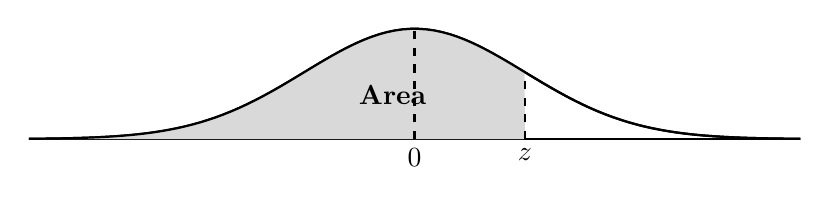
\begin{tikzpicture}[scale=1.4]
    % Draw baseline
    \draw (-3.5,0) -- (3.5,0);
    
    % Draw curve
    \draw[thick, domain=-3.5:3.5, samples=100] plot (\x, {exp(-0.5*\x*\x)});
    
    % Shaded Area from -infinity to z (positive z side)
    \fill[gray!30, domain=-3.5:1.0, samples=100] plot (\x, {exp(-0.5*\x*\x)}) -- (1.0,0) -- (-3.5,0) -- cycle;
    
    % Redraw curve over shading to keep the line crisp
    \draw[thick, domain=-3.5:3.5, samples=100] plot (\x, {exp(-0.5*\x*\x)});
    
    % Draw center dashed line and z line
    \draw[dashed, thick] (0,0) -- (0,1);
    \draw[dashed, thick] (1.0,0) -- (1.0,{exp(-0.5*1.0*1.0)});
    
    % Add labels
    \node[below] at (0,0) {0};
    \node[below] at (1.0,0) {$z$};
    \node at (-0.2, 0.4) {\textbf{Area}};
\end{tikzpicture}
\end{center}

\vspace{0.3cm}
\noindent\textbf{Table A.3 (continued)} Areas under the Normal Curve
\vspace{0.2cm}

% ================= DATA TABLE =================
\begin{center}
\small
\begin{longtable}{ccccccccccc}
\toprule\toprule
$z$ & .00 & .01 & .02 & .03 & .04 & .05 & .06 & .07 & .08 & .09 \\
\midrule
\endhead
\bottomrule\bottomrule
\endfoot
0.0 & 0.5000 & 0.5040 & 0.5080 & 0.5120 & 0.5160 & 0.5199 & 0.5239 & 0.5279 & 0.5319 & 0.5359 \\
0.1 & 0.5398 & 0.5438 & 0.5478 & 0.5517 & 0.5557 & 0.5596 & 0.5636 & 0.5675 & 0.5714 & 0.5753 \\
0.2 & 0.5793 & 0.5832 & 0.5871 & 0.5910 & 0.5948 & 0.5987 & 0.6026 & 0.6064 & 0.6103 & 0.6141 \\
0.3 & 0.6179 & 0.6217 & 0.6255 & 0.6293 & 0.6331 & 0.6368 & 0.6406 & 0.6443 & 0.6480 & 0.6517 \\
0.4 & 0.6554 & 0.6591 & 0.6628 & 0.6664 & 0.6700 & 0.6736 & 0.6772 & 0.6808 & 0.6844 & 0.6879 \\
0.5 & 0.6915 & 0.6950 & 0.6985 & 0.7019 & 0.7054 & 0.7088 & 0.7123 & 0.7157 & 0.7190 & 0.7224 \\
0.6 & 0.7257 & 0.7291 & 0.7324 & 0.7357 & 0.7389 & 0.7422 & 0.7454 & 0.7486 & 0.7517 & 0.7549 \\
0.7 & 0.7580 & 0.7611 & 0.7642 & 0.7673 & 0.7704 & 0.7734 & 0.7764 & 0.7794 & 0.7823 & 0.7852 \\
0.8 & 0.7881 & 0.7910 & 0.7939 & 0.7967 & 0.7995 & 0.8023 & 0.8051 & 0.8078 & 0.8106 & 0.8133 \\
0.9 & 0.8159 & 0.8186 & 0.8212 & 0.8238 & 0.8264 & 0.8289 & 0.8315 & 0.8340 & 0.8365 & 0.8389 \\
1.0 & 0.8413 & 0.8438 & 0.8461 & 0.8485 & 0.8508 & 0.8531 & 0.8554 & 0.8577 & 0.8599 & 0.8621 \\
1.1 & 0.8643 & 0.8665 & 0.8686 & 0.8708 & 0.8729 & 0.8749 & 0.8770 & 0.8790 & 0.8810 & 0.8830 \\
1.2 & 0.8849 & 0.8869 & 0.8888 & 0.8907 & 0.8925 & 0.8944 & 0.8962 & 0.8980 & 0.8997 & 0.9015 \\
1.3 & 0.9032 & 0.9049 & 0.9066 & 0.9082 & 0.9099 & 0.9115 & 0.9131 & 0.9147 & 0.9162 & 0.9177 \\
1.4 & 0.9192 & 0.9207 & 0.9222 & 0.9236 & 0.9251 & 0.9265 & 0.9278 & 0.9292 & 0.9306 & 0.9319 \\
1.5 & 0.9332 & 0.9345 & 0.9357 & 0.9370 & 0.9382 & 0.9394 & 0.9406 & 0.9418 & 0.9429 & 0.9441 \\
1.6 & 0.9452 & 0.9463 & 0.9474 & 0.9484 & 0.9495 & 0.9505 & 0.9515 & 0.9525 & 0.9535 & 0.9545 \\
1.7 & 0.9554 & 0.9564 & 0.9573 & 0.9582 & 0.9591 & 0.9599 & 0.9608 & 0.9616 & 0.9625 & 0.9633 \\
1.8 & 0.9641 & 0.9649 & 0.9656 & 0.9664 & 0.9671 & 0.9678 & 0.9686 & 0.9693 & 0.9699 & 0.9706 \\
1.9 & 0.9713 & 0.9719 & 0.9726 & 0.9732 & 0.9738 & 0.9744 & 0.9750 & 0.9756 & 0.9761 & 0.9767 \\
2.0 & 0.9772 & 0.9778 & 0.9783 & 0.9788 & 0.9793 & 0.9798 & 0.9803 & 0.9808 & 0.9812 & 0.9817 \\
2.1 & 0.9821 & 0.9826 & 0.9830 & 0.9834 & 0.9838 & 0.9842 & 0.9846 & 0.9850 & 0.9854 & 0.9857 \\
2.2 & 0.9861 & 0.9864 & 0.9868 & 0.9871 & 0.9875 & 0.9878 & 0.9881 & 0.9884 & 0.9887 & 0.9890 \\
2.3 & 0.9893 & 0.9896 & 0.9898 & 0.9901 & 0.9904 & 0.9906 & 0.9909 & 0.9911 & 0.9913 & 0.9916 \\
2.4 & 0.9918 & 0.9920 & 0.9922 & 0.9925 & 0.9927 & 0.9929 & 0.9931 & 0.9932 & 0.9934 & 0.9936 \\
2.5 & 0.9938 & 0.9940 & 0.9941 & 0.9943 & 0.9945 & 0.9946 & 0.9948 & 0.9949 & 0.9951 & 0.9952 \\
2.6 & 0.9953 & 0.9955 & 0.9956 & 0.9957 & 0.9959 & 0.9960 & 0.9961 & 0.9962 & 0.9963 & 0.9964 \\
2.7 & 0.9965 & 0.9966 & 0.9967 & 0.9968 & 0.9969 & 0.9970 & 0.9971 & 0.9972 & 0.9973 & 0.9974 \\
2.8 & 0.9974 & 0.9975 & 0.9976 & 0.9977 & 0.9977 & 0.9978 & 0.9979 & 0.9979 & 0.9980 & 0.9981 \\
2.9 & 0.9981 & 0.9982 & 0.9982 & 0.9983 & 0.9984 & 0.9984 & 0.9985 & 0.9985 & 0.9986 & 0.9986 \\
3.0 & 0.9987 & 0.9987 & 0.9987 & 0.9987 & 0.9988 & 0.9988 & 0.9989 & 0.9989 & 0.9990 & 0.9990 \\
3.1 & 0.9990 & 0.9991 & 0.9991 & 0.9991 & 0.9992 & 0.9992 & 0.9992 & 0.9992 & 0.9993 & 0.9993 \\
3.2 & 0.9993 & 0.9993 & 0.9994 & 0.9994 & 0.9994 & 0.9994 & 0.9994 & 0.9995 & 0.9995 & 0.9995 \\
3.3 & 0.9995 & 0.9995 & 0.9995 & 0.9996 & 0.9996 & 0.9996 & 0.9996 & 0.9996 & 0.9996 & 0.9997 \\
3.4 & 0.9997 & 0.9997 & 0.9997 & 0.9997 & 0.9997 & 0.9997 & 0.9997 & 0.9997 & 0.9997 & 0.9998 \\
\end{longtable}
\end{center}

\item The mean weekly sale of chocolate bars was 153.7 bars/store. After an advertising campaign, 29 stores averaged 169.4 with standard deviation 19.7. Was the advertising successful at 5\% significance?


% ================= STUDENT'S T DISTRIBUTION =================
\begin{center}
\begin{minipage}{0.45\textwidth}
    \centering
    \textbf{\large Percentile Values ($t_p$)} \\
    \vspace{0.2cm}
    \textbf{for} \\
    \vspace{0.2cm}
    \textbf{Student's $t$ Distribution} \\
    \vspace{0.2cm}
    \textbf{with $\nu$ Degrees of Freedom} \\
    \vspace{0.2cm}
    \textbf{(shaded area = $p$)}
\end{minipage}
\hfill
\begin{minipage}{0.45\textwidth}
    \centering
    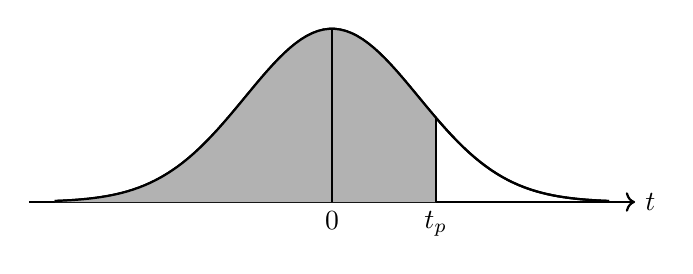
\begin{tikzpicture}[scale=1.1]
        % Draw baseline
        \draw[->, thick] (-3.5,0) -- (3.5,0) node[right] {$t$};
        
        % Draw curve
        \draw[thick, domain=-3.2:3.2, samples=100] plot (\x, {2.0*exp(-0.5*\x*\x)});
        
        % Shaded Area (from left to t_p)
        \fill[gray!60, domain=-3.2:1.2, samples=100] plot (\x, {2.0*exp(-0.5*\x*\x)}) -- (1.2,0) -- (-3.2,0) -- cycle;
        
        % Redraw curve over shading
        \draw[thick, domain=-3.2:3.2, samples=100] plot (\x, {2.0*exp(-0.5*\x*\x)});
        
        % Draw center line and t_p line
        \draw[thick] (0,0) -- (0,2.0);
        \draw[thick] (1.2,0) -- (1.2,{2.0*exp(-0.5*1.2*1.2)});
        
        % Add labels
        \node[below] at (0,0) {0};
        \node[below] at (1.2,0) {$t_p$};
    \end{tikzpicture}
\end{minipage}
\end{center}
\vspace{0.5cm}

\begin{center}
\begin{longtable}{c | ccccc | ccccc}
\toprule
$\nu$ & $t_{.995}$ & $t_{.99}$ & $t_{.975}$ & $t_{.95}$ & $t_{.90}$ & $t_{.80}$ & $t_{.75}$ & $t_{.70}$ & $t_{.60}$ & $t_{.55}$ \\
\midrule
\endhead

\midrule
\multicolumn{11}{r}{{Continued on next page}} \\
\bottomrule
\endfoot

\bottomrule
\endlastfoot

1 & 63.66 & 31.82 & 12.71 & 6.31 & 3.08 & 1.376 & 1.000 & .727 & .325 & .158 \\
2 & 9.92 & 6.96 & 4.30 & 2.92 & 1.89 & 1.061 & .816 & .617 & .289 & .142 \\
3 & 5.84 & 4.54 & 3.18 & 2.35 & 1.64 & .978 & .765 & .584 & .277 & .137 \\
4 & 4.60 & 3.75 & 2.78 & 2.13 & 1.53 & .941 & .741 & .569 & .271 & .134 \\
5 & 4.03 & 3.36 & 2.57 & 2.02 & 1.48 & .920 & .727 & .559 & .267 & .132 \\
6 & 3.71 & 3.14 & 2.45 & 1.94 & 1.44 & .906 & .718 & .553 & .265 & .131 \\
7 & 3.50 & 3.00 & 2.36 & 1.89 & 1.41 & .896 & .711 & .549 & .263 & .130 \\
8 & 3.36 & 2.90 & 2.31 & 1.86 & 1.40 & .889 & .706 & .546 & .262 & .130 \\
9 & 3.25 & 2.82 & 2.26 & 1.83 & 1.38 & .883 & .703 & .543 & .261 & .129 \\
10 & 3.17 & 2.76 & 2.23 & 1.81 & 1.37 & .879 & .700 & .542 & .260 & .129 \\
11 & 3.11 & 2.72 & 2.20 & 1.80 & 1.36 & .876 & .697 & .540 & .260 & .129 \\
12 & 3.05 & 2.68 & 2.18 & 1.78 & 1.36 & .873 & .695 & .539 & .259 & .128 \\
13 & 3.01 & 2.65 & 2.16 & 1.77 & 1.35 & .870 & .694 & .538 & .259 & .128 \\
14 & 2.98 & 2.62 & 2.14 & 1.76 & 1.35 & .868 & .692 & .537 & .258 & .128 \\
15 & 2.95 & 2.60 & 2.13 & 1.75 & 1.34 & .866 & .691 & .536 & .258 & .128 \\
16 & 2.92 & 2.58 & 2.12 & 1.75 & 1.34 & .865 & .690 & .535 & .258 & .128 \\
17 & 2.90 & 2.57 & 2.11 & 1.74 & 1.33 & .863 & .689 & .534 & .257 & .128 \\
18 & 2.88 & 2.55 & 2.10 & 1.73 & 1.33 & .862 & .688 & .534 & .257 & .127 \\
19 & 2.86 & 2.54 & 2.09 & 1.73 & 1.33 & .861 & .688 & .533 & .257 & .127 \\
20 & 2.85 & 2.53 & 2.09 & 1.72 & 1.33 & .860 & .687 & .533 & .257 & .127 \\
21 & 2.83 & 2.52 & 2.08 & 1.72 & 1.32 & .859 & .686 & .532 & .257 & .127 \\
22 & 2.82 & 2.51 & 2.07 & 1.72 & 1.32 & .858 & .686 & .532 & .256 & .127 \\
23 & 2.81 & 2.50 & 2.07 & 1.71 & 1.32 & .858 & .685 & .532 & .256 & .127 \\
24 & 2.80 & 2.49 & 2.06 & 1.71 & 1.32 & .857 & .685 & .531 & .256 & .127 \\
25 & 2.79 & 2.49 & 2.06 & 1.71 & 1.32 & .856 & .684 & .531 & .256 & .127 \\
26 & 2.78 & 2.48 & 2.06 & 1.71 & 1.31 & .856 & .684 & .531 & .256 & .127 \\
27 & 2.77 & 2.47 & 2.05 & 1.70 & 1.31 & .855 & .684 & .531 & .256 & .127 \\
28 & 2.76 & 2.47 & 2.05 & 1.70 & 1.31 & .855 & .683 & .530 & .256 & .127 \\
29 & 2.76 & 2.46 & 2.05 & 1.70 & 1.31 & .854 & .683 & .530 & .256 & .127 \\
30 & 2.75 & 2.46 & 2.04 & 1.70 & 1.31 & .854 & .683 & .530 & .256 & .127 \\
40 & 2.70 & 2.42 & 2.02 & 1.68 & 1.30 & .851 & .681 & .529 & .255 & .126 \\
60 & 2.66 & 2.39 & 2.00 & 1.67 & 1.30 & .848 & .679 & .527 & .254 & .126 \\
120 & 2.62 & 2.36 & 1.98 & 1.66 & 1.29 & .845 & .677 & .526 & .254 & .126 \\
$\infty$ & 2.58 & 2.33 & 1.96 & 1.645 & 1.28 & .842 & .674 & .524 & .253 & .126 \\
\end{longtable}

\vspace{0.5cm}
\small{\textit{Source: R. A. Fisher and F. Yates, Statistical Tables for Biological, Agricultural and Medical Research (5th edition), Table III, Oliver and Boyd Ltd., Edinburgh, by permission of the authors and publishers.}}
\end{center}

\mk{10} \yr{MATH 241 | L-2/T-1 | 2015--16}

\item A bulb manufacturing company claims the average longevity of their bulbs is 4 years with a standard deviation of 0.16 years. A random sample of 10 bulbs gave a mean longevity of 3.45 years. Does the sample mean justify the manufacturer's claim at the 5\% level of significance?

\mk{15} \yr{MATH 241 | L-2/T-1 | 2014--15}


% ================= STUDENT'S T DISTRIBUTION =================
\begin{center}
\begin{minipage}{0.45\textwidth}
    \centering
    \textbf{\large Percentile Values ($t_p$)} \\
    \vspace{0.2cm}
    \textbf{for} \\
    \vspace{0.2cm}
    \textbf{Student's $t$ Distribution} \\
    \vspace{0.2cm}
    \textbf{with $\nu$ Degrees of Freedom} \\
    \vspace{0.2cm}
    \textbf{(shaded area = $p$)}
\end{minipage}
\hfill
\begin{minipage}{0.45\textwidth}
    \centering
    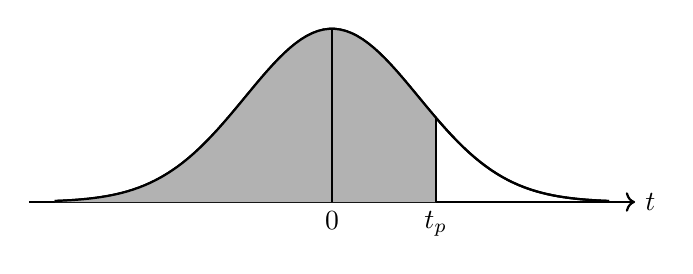
\begin{tikzpicture}[scale=1.1]
        % Draw baseline
        \draw[->, thick] (-3.5,0) -- (3.5,0) node[right] {$t$};
        
        % Draw curve
        \draw[thick, domain=-3.2:3.2, samples=100] plot (\x, {2.0*exp(-0.5*\x*\x)});
        
        % Shaded Area (from left to t_p)
        \fill[gray!60, domain=-3.2:1.2, samples=100] plot (\x, {2.0*exp(-0.5*\x*\x)}) -- (1.2,0) -- (-3.2,0) -- cycle;
        
        % Redraw curve over shading
        \draw[thick, domain=-3.2:3.2, samples=100] plot (\x, {2.0*exp(-0.5*\x*\x)});
        
        % Draw center line and t_p line
        \draw[thick] (0,0) -- (0,2.0);
        \draw[thick] (1.2,0) -- (1.2,{2.0*exp(-0.5*1.2*1.2)});
        
        % Add labels
        \node[below] at (0,0) {0};
        \node[below] at (1.2,0) {$t_p$};
    \end{tikzpicture}
\end{minipage}
\end{center}
\vspace{0.5cm}

\begin{center}
\begin{longtable}{c | ccccc | ccccc}
\toprule
$\nu$ & $t_{.995}$ & $t_{.99}$ & $t_{.975}$ & $t_{.95}$ & $t_{.90}$ & $t_{.80}$ & $t_{.75}$ & $t_{.70}$ & $t_{.60}$ & $t_{.55}$ \\
\midrule
\endhead

\midrule
\multicolumn{11}{r}{{Continued on next page}} \\
\bottomrule
\endfoot

\bottomrule
\endlastfoot

1 & 63.66 & 31.82 & 12.71 & 6.31 & 3.08 & 1.376 & 1.000 & .727 & .325 & .158 \\
2 & 9.92 & 6.96 & 4.30 & 2.92 & 1.89 & 1.061 & .816 & .617 & .289 & .142 \\
3 & 5.84 & 4.54 & 3.18 & 2.35 & 1.64 & .978 & .765 & .584 & .277 & .137 \\
4 & 4.60 & 3.75 & 2.78 & 2.13 & 1.53 & .941 & .741 & .569 & .271 & .134 \\
5 & 4.03 & 3.36 & 2.57 & 2.02 & 1.48 & .920 & .727 & .559 & .267 & .132 \\
6 & 3.71 & 3.14 & 2.45 & 1.94 & 1.44 & .906 & .718 & .553 & .265 & .131 \\
7 & 3.50 & 3.00 & 2.36 & 1.89 & 1.41 & .896 & .711 & .549 & .263 & .130 \\
8 & 3.36 & 2.90 & 2.31 & 1.86 & 1.40 & .889 & .706 & .546 & .262 & .130 \\
9 & 3.25 & 2.82 & 2.26 & 1.83 & 1.38 & .883 & .703 & .543 & .261 & .129 \\
10 & 3.17 & 2.76 & 2.23 & 1.81 & 1.37 & .879 & .700 & .542 & .260 & .129 \\
11 & 3.11 & 2.72 & 2.20 & 1.80 & 1.36 & .876 & .697 & .540 & .260 & .129 \\
12 & 3.05 & 2.68 & 2.18 & 1.78 & 1.36 & .873 & .695 & .539 & .259 & .128 \\
13 & 3.01 & 2.65 & 2.16 & 1.77 & 1.35 & .870 & .694 & .538 & .259 & .128 \\
14 & 2.98 & 2.62 & 2.14 & 1.76 & 1.35 & .868 & .692 & .537 & .258 & .128 \\
15 & 2.95 & 2.60 & 2.13 & 1.75 & 1.34 & .866 & .691 & .536 & .258 & .128 \\
16 & 2.92 & 2.58 & 2.12 & 1.75 & 1.34 & .865 & .690 & .535 & .258 & .128 \\
17 & 2.90 & 2.57 & 2.11 & 1.74 & 1.33 & .863 & .689 & .534 & .257 & .128 \\
18 & 2.88 & 2.55 & 2.10 & 1.73 & 1.33 & .862 & .688 & .534 & .257 & .127 \\
19 & 2.86 & 2.54 & 2.09 & 1.73 & 1.33 & .861 & .688 & .533 & .257 & .127 \\
20 & 2.85 & 2.53 & 2.09 & 1.72 & 1.33 & .860 & .687 & .533 & .257 & .127 \\
21 & 2.83 & 2.52 & 2.08 & 1.72 & 1.32 & .859 & .686 & .532 & .257 & .127 \\
22 & 2.82 & 2.51 & 2.07 & 1.72 & 1.32 & .858 & .686 & .532 & .256 & .127 \\
23 & 2.81 & 2.50 & 2.07 & 1.71 & 1.32 & .858 & .685 & .532 & .256 & .127 \\
24 & 2.80 & 2.49 & 2.06 & 1.71 & 1.32 & .857 & .685 & .531 & .256 & .127 \\
25 & 2.79 & 2.49 & 2.06 & 1.71 & 1.32 & .856 & .684 & .531 & .256 & .127 \\
26 & 2.78 & 2.48 & 2.06 & 1.71 & 1.31 & .856 & .684 & .531 & .256 & .127 \\
27 & 2.77 & 2.47 & 2.05 & 1.70 & 1.31 & .855 & .684 & .531 & .256 & .127 \\
28 & 2.76 & 2.47 & 2.05 & 1.70 & 1.31 & .855 & .683 & .530 & .256 & .127 \\
29 & 2.76 & 2.46 & 2.05 & 1.70 & 1.31 & .854 & .683 & .530 & .256 & .127 \\
30 & 2.75 & 2.46 & 2.04 & 1.70 & 1.31 & .854 & .683 & .530 & .256 & .127 \\
40 & 2.70 & 2.42 & 2.02 & 1.68 & 1.30 & .851 & .681 & .529 & .255 & .126 \\
60 & 2.66 & 2.39 & 2.00 & 1.67 & 1.30 & .848 & .679 & .527 & .254 & .126 \\
120 & 2.62 & 2.36 & 1.98 & 1.66 & 1.29 & .845 & .677 & .526 & .254 & .126 \\
$\infty$ & 2.58 & 2.33 & 1.96 & 1.645 & 1.28 & .842 & .674 & .524 & .253 & .126 \\
\end{longtable}

\vspace{0.5cm}
\small{\textit{Source: R. A. Fisher and F. Yates, Statistical Tables for Biological, Agricultural and Medical Research (5th edition), Table III, Oliver and Boyd Ltd., Edinburgh, by permission of the authors and publishers.}}
\end{center}


\item Talcum powder is packed into tins by machines. A random sample of 11 tins has contents (in lbs): 0.44, 0.51, 0.49, 0.52, 0.45, 0.48, 0.46, 0.45, 0.47, 0.45, 0.47. Test whether the average packing can be taken to be 0.5 lbs at 5\% level of significance. (Given: $t=\pm2.23$.)
\mk{20} \yr{MATH 241 | L-2/T-1 | 2013--14}

\item A survey of 320 families with 5 children each revealed the following distribution. Is the result consistent with the hypothesis that male and female births are equally probable? Use 5\% level of significance. (Given: for $\nu=5$, $\chi^{2}=11.07$.)
\begin{center}
\begin{tabular}{lrrrrrr}
\toprule
No.\ of boys  & 5  & 4  & 3   & 2  & 1  & 0 \\
No.\ of girls & 0  & 1  & 2   & 3  & 4  & 5 \\
\midrule
No.\ of families & 18 & 56 & 110 & 88 & 40 & 8 \\
\bottomrule
\end{tabular}
\end{center}
\mk{15} \yr{MATH 241 | L-2/T-1 | 2013--14}

\item A survey of 640 families with 5 children each revealed the following distribution. Is this result consistent with the hypothesis that male and female births are equally probable? Use 5\% level of significance. (Given: for $\nu=5$, $\chi^{2}_{0.05}=11.07$.)
\begin{center}
\begin{tabular}{lrrrrrr}
\toprule
No.\ of boys  & 5  & 4   & 3   & 2   & 1  & 0  \\
No.\ of girls & 0  & 1   & 2   & 3   & 4  & 5  \\
\midrule
No.\ of families & 28 & 112 & 220 & 176 & 80 & 24 \\
\bottomrule
\end{tabular}
\end{center}
\mk{15} \yr{MATH 241 | L-2/T-1 | 2012--13}

\item In a survey of buying habits, 500 women shoppers chosen at random in supermarket A have an average weekly food expenditure of Tk.\,500 with a standard deviation of Tk.\,80. Another group of 500 women shoppers in supermarket B have an average of Tk.\,440 with a standard deviation of Tk.\,90. Test at 10\% level of significance whether the average weekly food expenditures are equal.
\mk{17} \yr{MATH 241 | L-2/T-1 | 2012--13}

\item Explain Type I and Type II errors. A sample of 9 items had values: 50, 48, 49, 53, 52, 47, 45, 46, 51. Can this sample be regarded as taken from a population with mean 47, at 5\% level of significance? (Given: for $\nu=8$, $t_{0.05}=3.355$.)
\mk{17} \yr{MATH 241 | L-2/T-1 | 2011--12}

\item Five coins are tossed 3200 times and the number of heads appearing each time is noted. Test the hypothesis that the coins are unbiased at 5\% level of significance. (Given: for $\nu=5$, $\chi^{2}_{0.05}=11.07$.)
\begin{center}
\begin{tabular}{lrrrrrrr}
\toprule
No.\ of heads & 0 & 1 & 2 & 3 & 4 & 5 \\
\midrule
Frequency & 80 & 570 & 1100 & 900 & 500 & 50 \\
\bottomrule
\end{tabular}
\end{center}
\mk{18} \yr{MATH 241 | L-2/T-1 | 2011--12}

\item The mean and standard deviation of GPA scores from a random sample of 40 students were 2.8 and 0.35 respectively. Can we conclude that the sample has come from a population with mean 2.4? Use a 1\% level of significance. Also compute a 99\% confidence interval for the population mean. (Given: $z=\pm2.58$.)


\item A random sample of 20 servings of a cereal has a mean sodium content of 244 mg and standard deviation 24.5 mg. Does this suggest at the 0.05 level that the average sodium content exceeds 220 mg?
\mk{15} \yr{MATH 245 | L-2/T-1 | }

\end{enumerate}
\label{sub:s9-regression}

\begin{enumerate}

\item The following table shows the experience ($X$) and the performance rating ($Y$) of 5 persons:
\begin{center}
\begin{tabular}{lccccc}
\toprule
$X$ & 16 & 12 & 18 & 4 & 3 \\
\midrule
$Y$ & 87 & 88 & 89 & 68 & 58 \\
\bottomrule
\end{tabular}
\end{center}
\begin{enumerate}
  \item Fit a linear regression model for $Y$ on $X$.
  \item Find SSR and SST.
\end{enumerate}
\mk{15} \yr{MATH 245 | L-2/T-1 | 2020--21}

\item Find the two regression lines and the coefficient of correlation from the data:
\begin{center}
\begin{tabular}{lccccccccc}
\toprule
$X$ & 105 & 112 & 104 & 114 & 117 & 108 & 106 & 117 & 111 \\
\midrule
$Y$ & 58  & 56  & 47  & 46  & 51  & 64  & 66  & 50  & 55  \\
\bottomrule
\end{tabular}
\end{center}
\mk{20} \yr{MATH 241 | L-2/T-1 | 2011--12}

\item The marks in Economics (out of 50) and Business (out of 50) for 10 students are:
\begin{center}
\begin{tabular}{lcccccccccc}
\toprule
Economics & 47 & 38 & 34 & 44 & 32 & 41 & 35 & 32 & 42 & 30 \\
\midrule
Business  & 38 & 34 & 42 & 39 & 34 & 33 & 30 & 41 & 38 & 28 \\
\bottomrule
\end{tabular}
\end{center}
Calculate the two regression equations and regression coefficients. Estimate the marks in Economics if a student scored 36 in Business, and the marks in Business if another scored 44 in Economics. Also comment on the correlation between the two subjects.
\mk{20} \yr{MATH 241 | L-2/T-1 | 2012--13}

\item Calculate the two regression equations and the coefficient of correlation from the data below. Also estimate the most likely age of husband when wife's age is 24.
\begin{center}
\begin{tabular}{lcccccccc}
\toprule
Age of husband & 22 & 25 & 28 & 31 & 35 & 32 & 37 & 39 \\
\midrule
Age of wife    & 19 & 18 & 22 & 29 & 31 & 23 & 30 & 33 \\
\bottomrule
\end{tabular}
\end{center}
\mk{20} \yr{MATH 241 | L-2/T-1 | 2013--14}

\item Find the regression line of $Y$ on $X$ and $X$ on $Y$. Find also the correlation coefficient between $X$ and $Y$.
\begin{center}
\begin{tabular}{lccccccc}
\toprule
$X$ & 42 & 44 & 58 & 55 & 89 & 98 & 66 \\
\midrule
$Y$ & 56 & 49 & 53 & 58 & 65 & 76 & 51 \\
\bottomrule
\end{tabular}
\end{center}
\mk{20} \yr{MATH 241 | L-2/T-1 | 2014--15}

\item The following table shows the experience ($X$) and the performance rating ($Y$) of 5 persons:
\begin{center}
\begin{tabular}{lccccc}
\toprule
$X$ & 16 & 12 & 18 & 4 & 3 \\
\midrule
$Y$ & 87 & 88 & 89 & 68 & 58 \\
\bottomrule
\end{tabular}
\end{center}
\begin{enumerate}
  \item Fit a linear regression model for $Y$ on $X$.
  \item Find SSR and SST.
  \item Is the linear model appropriate? Justify using the coefficient of determination.
\end{enumerate}
\mk{18} \yr{MATH 245 | L-2/T-1 | 2016--17}

\item Find the regression equation of capacity utilisation on production given $r=0.62$:
\begin{center}
\begin{tabular}{lcc}
\toprule
 & \textbf{Average} & \textbf{Standard deviation} \\
\midrule
Production & 35.6 & 10.5 \\
Capacity utilisation & 84.8 & 8.5 \\
\bottomrule
\end{tabular}
\end{center}
Also estimate the production when capacity utilisation is 70\%.
\mk{20} \yr{MATH 245 | L-2/T-1 | 2018--19}

\item A factory manager wants to find a measure which he can use to fix the monthly
income for persons applying for a job in a production department. 
A factory manager collected data from 9 persons on years of service and monthly income:
\begin{center}
\begin{tabular}{lrrrrrrrrr}
\toprule
\textbf{Years of service} & 10 & 8 & 9 & 5 & 7 & 6 & 12 & 11 & 13 \\
\midrule
\textbf{Income ('000)} & 17 & 12 & 14 & 8 & 10 & 9 & 20 & 18 & 22 \\
\bottomrule
\end{tabular}
\end{center}
(i) Calculate the regression equations and the correlation coefficient. (ii) What initial salary would you recommend for a person with 15 years of experience?
\mk{17} \yr{MATH 241 | L-2/T-1 | 2015--16}

\item The distance to transmitter ($X$) and wireless signal strength ($Y$) data:
\begin{center}
\begin{tabular}{lrrrrrrrrrr}
\toprule
$X$ (m) & 13 & 12 & 17 & 19 & 14 & 15 & 15 & 8 & 13 & 3 \\
\midrule
$Y$ (dB) & 34.4 & 38.4 & 30.4 & 29.7 & 30.1 & 33.9 & 32.8 & 35.2 & 34.9 & 36.8 \\
\bottomrule
\end{tabular}
\end{center}
Find the regression line of $Y$ on $X$ and predict the signal strength at 10 m distance.
\mk{17} \yr{MATH 245 | L-2/T-1 | 2019--20}


\item It is important that scientific researchers in the area of forest products be able to study correlation among the anatomy and mechanical properties of trees. For the study Quantitative Anatomical Characteristics of Plantation Grown Loblolly Pine (Pinus Taeda L.) and Cottonwood (Populus deltoids Bart. Ex Marsh.) and their relationships to mechanical properties, conducted by the Department of Forestry and Forest Products at Virginia Tech, 15 loblolly pines are randomly selected for investigation. The resulting data on the specific gravity and the modulus of rupture is shown below:
\begin{center}
  \begin{tabular}{|c|c|}
\hline
Specific Gravity, x (g/cm$^3$) & Modulus of Rupture, y (kPa) \\ \hline
0.414 & 29,186 \\ \hline
0.383 & 29,266 \\ \hline
0.399 & 26,215 \\ \hline
0.402 & 30,162 \\ \hline
0.442 & 38,867 \\ \hline
0.422 & 37,831 \\ \hline
0.466 & 44,576 \\ \hline
0.500 & 46,097 \\ \hline
0.514 & 59,698 \\ \hline
0.530 & 67,705 \\ \hline
0.569 & 66,088 \\ \hline
0.558 & 78,486 \\ \hline
0.577 & 89,869 \\ \hline
0.572 & 77,369 \\ \hline
0.548 & 67,095 \\ \hline
\end{tabular}
\end{center}

\begin{enumerate}
  \item Find both the regression coefficient.
  \item Compute the interpret the sample correlation coefficient.
\end{enumerate}
\mk{20} \yr{MATH 245 | L-2/T-1 | 2021--22}

\end{enumerate}

%%──────────────────────────────────────────────────────────────────────
\subtopic{cG}{Analysis of Variance (ANOVA)}
\label{sub:s9-anova}

\begin{enumerate}\item A merchandising company wishes to test whether its 3 salesman A, B and C tend to make sales of the same size or whether they differ selling ability as measures by the average size of their sales. During the last week, out of 14 sales, A made 5, B made 4 and C made 5 calls. The following are the weekly sales (in Tk thousand) record of 3 salesman:
\begin{center}
  \begin{tabular}{|c|c|c|}
\hline
A   & B   & C   \\ \hline
300 & 600 & 700 \\ \hline
400 & 300 & 300 \\ \hline
300 & 300 & 400 \\ \hline
500 & 400 & 600 \\ \hline
0   & --  & 500 \\ \hline
\end{tabular}
\end{center}

\vspace{0.2cm}

Test whether the three salesman's average sales differ in size. (Given that $F_{(2,11)}$ at 5\% level of significance = 3.98)
\mk{18} \yr{MATH 245 | L-2/T-1 | 2021--22}

\end{enumerate}


%% ══════════════════════════════════════════════════════════════════════
%%  PART VIII — COORDINATE GEOMETRY
%% ══════════════════════════════════════════════════════════════════════
\secdivider{Coordinate Geometry}{Straight Lines, Circles, Conics, 3D Geometry}{cH}

\section{S10. Coordinate Geometry}
\label{sec:S10}
\markboth{S10. Coordinate Geometry}{}

%%──────────────────────────────────────────────────────────────────────
\subtopic{cH}{Straight Lines}
\label{sub:s10-lines}

\begin{enumerate}\item Show that the lines joining the origin to the intersection of $x^{2}+y^{2}+19x+4y-3=0$ and $3x+4y=1$ are at right angles.
\mk{17} \yr{MATH 141 | L-1/T-1 | 2003--04}

\end{enumerate}

%%──────────────────────────────────────────────────────────────────────
\subtopic{cH}{Pair of Straight Lines}
\label{sub:s10-pairlines}

\begin{enumerate}\item Find the point of intersection of the pair of straight lines $10x^{2}-13xy+4y^{2}+13x-14y=30$. Hence compute the area of the triangle formed by these lines and the $x$-axis.
\mk{12} \yr{MATH 145 | L-1/T-1 | 2020--21}


\item Prove that the straight lines represented by $ax^{2}+2hxy+by^{2}+2gx+2fy+c=0$ are equidistant from the origin if $f^{4}-g^{4}=c(bf^{2}-ag^{2})$.
\mk{15} \yr{MATH 145 | L-1/T-2 | 2019--20}

\item Show that the equation $ax^{2}+2hxy+by^{2}+2gx+2fy+c=0$ represents two parallel lines if $\dfrac{a}{h}=\dfrac{h}{b}=\dfrac{g}{f}$, and then the distance between them is $2\sqrt{\dfrac{g^{2}-ac}{a(a+b)}}$.
\mk{13} \yr{MATH 145 | L-1/T-1 | 2018--19}

\item Show that $2x^{2}-7xy+3y^{2}+x+7y=6$ represents a pair of straight lines. Find the point of intersection and the angle made by them.
\mk{10} \yr{MATH 145 | L-1/T-1 | 2017--18}

\item If $ax^{2}+2hxy+by^{2}+2gx+2fy+c=0$ represents a pair of straight lines, show that the area of the triangle formed by these lines and the axis of $x$ is $\dfrac{g^{2}-ac}{a\sqrt{h^{2}-ab}}$.
\mk{12} \yr{MATH 145 | L-1/T-1 | 2016--17}

\item Prove the necessary and sufficient condition that two of the lines represented by $ay^{4}+bxy^{3}+cx^{2}y^{2}+dx^{3}y+ex^{4}=0$ are at right angles is $(b+d)(ad+bc)+(e-a)^{2}(a+c+e)=0$.
\mk{11} \yr{MATH 145 | L-1/T-1 | 2016--17}

\item Show that the equation $ax^{2}+2hxy+by^{2}+2gx+2fy+c=0$ represents two parallel lines if $\dfrac{a}{h}=\dfrac{h}{b}=\dfrac{g}{f}$ and that the distance between them is $2\sqrt{\dfrac{g^{2}-ac}{a(a+b)}}$.
\mk{18} \yr{MATH 145 | L-1/T-1 | 2015--16}

\item Show that the equation $ax^{2}+2hxy+by^{2}+2gx+2fy+c=0$ represents a pair of parallel straight lines if $\dfrac{a}{h}=\dfrac{h}{b}=\dfrac{g}{f}$ and that the distance between them is $2\sqrt{\dfrac{g^{2}-ac}{a(a+b)}}$.
\mk{18} \yr{MATH 141 | L-1/T-1 | 2014--15}

\item Prove that $(ax+by)({\alpha}x+{\beta}y)+kxy-(\alpha+a)x-(\beta+b)y+1=0$ represents a pair of straight lines if $k=(\alpha-a)(\beta-b)$. Find their point of intersection.
\mk{18} \yr{MATH 141 | L-1/T-1 | 2014--15}

\item Find the equation of the pair of lines joining the origin to the points of intersection of $\dfrac{x}{a}+\dfrac{y}{b}=1$ and the circle $x^{2}+y^{2}=c^{2}$, and deduce that the line is tangent to the circle if $\dfrac{1}{a^{2}}+\dfrac{1}{b^{2}}=\dfrac{1}{c^{2}}$.
\mk{17} \yr{MATH 141 | L-1/T-1 | 2014--15}

\item If one of the straight lines given by $ax^{2}+2hxy+by^{2}=0$ coincides with one of the lines given by $a_{1}x^{2}+2h_{1}xy+b_{1}y^{2}=0$ and the other lines represented by them are perpendicular, prove that
\[
\frac{ha_{1}b_{1}}{b_{1}-a_{1}}=\frac{h_{1}ab}{b-a}=\frac{1}{2}\sqrt{-aa_{1}bb_{1}}.
\]
\mk{18} \yr{MATH 141 | L-1/T-1 | 2013--14}

\item Prove that the straight lines joining the origin to the points of intersection of the line $kx+hy=2hk$ with the curve $(x-h)^{2}+(y-k)^{2}=c^{2}$ are at right angles if $h^{2}+k^{2}=c^{2}$.
\mk{17} \yr{MATH 141 | L-1/T-1 | 2013--14}

\item If the equation $ax^{2}+2hxy+by^{2}+2gx+2fy+c=0$ represents a pair of straight lines, show that the distance of their point of intersection from the origin is $\sqrt{\dfrac{c(a+b)-f^{2}-g^{2}}{ab-h^{2}}}$.
\mk{10} \yr{MATH 141 | L-1/T-1 | 2012--13}

\item If one of the lines represented by $ax^{3}+bx^{2}y+cxy^{2}+dy^{3}=0$ bisects the angle between the other two, show that $(3a+c)^{2}(bc+2cd-3ad)=(b+3d)^{2}(bc+2ab-3ad)$.
\mk{15} \yr{MATH 141 | L-1/T-1 | 2012--13}

\item Find the angle between the lines joining the origin to the points of intersection of the curve $x^{2}+y^{2}+19x+4y-3=0$ and the line $3x+4y=1$.
\mk{10} \yr{MATH 141 | L-1/T-1 | 2011--12}

\item If one of the lines $ax^{2}+2hxy+by^{2}=0$ is perpendicular to one of the lines $a'x^{2}+2h'xy+b'y^{2}=0$, prove that $(aa'-bb')^{2}+4(a'h+bh')(ah'+b'h)=0$.
\mk{10} \yr{MATH 141 | L-1/T-1 | 2011--12}

\item If $ax^{2}+2hxy+by^{2}+2gx+2fy+c=0$ represents a pair of straight lines, show that the area of the triangle formed by their bisectors and the axis of $x$ is $\dfrac{\sqrt{(a-b)^{2}+4h^{2}}}{2h}\cdot\dfrac{ac-g^{2}}{ab-h^{2}}$.
\mk{15} \yr{MATH 141 | L-1/T-1 | 2011--12}

\item Find the value of $k$ so that the lines which join the origin to the points of intersection of the line $y-x-k=0$ and the curve $x^{2}+y^{2}+4x-6y-36=0$ may be at right angles.
\mk{8} \yr{MATH 141 | L-1/T-1 | 2010--11}

\item Show that the distance from the origin to the orthocentre of the triangle formed by the straight line $\dfrac{x}{\alpha}+\dfrac{y}{\beta}=1$ and $ax^{2}+2hxy+by^{2}=0$ is
$\dfrac{(a+b)\alpha\beta\sqrt{\alpha^{2}+\beta^{2}}}{a\alpha^{2}+2h\alpha\beta+b\beta^{2}}$.
\mk{15} \yr{MATH 141 | L-1/T-1 | 2010--11}

\item If one of the straight lines given by $ax^{2}+2hxy+by^{2}=0$ coincides with one of the lines given by $a_{1}x^{2}+2h_{1}xy+b_{1}y^{2}=0$ and the other lines represented by them are perpendicular, then prove that
\[
\frac{ha_{1}b_{1}}{b_{1}-a_{1}}=\frac{h_{1}ab}{b-a}=\frac{1}{2}\sqrt{-aa_{1}bb_{1}}.
\]
\mk{20} \yr{MATH 141 | L-1/T-1 | 2010--11}

\item Show that the equation $ax^{2}+2hxy+by^{2}+2gx+2fy+c=0$ represents two parallel lines if $\dfrac{a}{h}=\dfrac{h}{b}=\dfrac{g}{f}$. Also show that the distance between them is $2\sqrt{\dfrac{g^{2}-ac}{a(a+b)}}$.
\mk{18} \yr{MATH 141 | L-1/T-1 | 2008--09}

\item If one of the straight lines given by $ax^{2}+2hxy+by^{2}=0$ coincides with one of those given by $a_{1}x^{2}+2h_{1}xy+b_{1}y^{2}=0$ and the other lines represented by them be perpendicular, prove that
\[
\frac{h_{1}a_{1}b_{1}}{b_{1}-a_{1}}=\frac{h_{1}ab}{b-a}=\frac{1}{2}\sqrt{-aa_{1}bb_{1}}.
\]
\mk{18} \yr{MATH 141 | L-1/T-1 | 2008--09}

\item Find the equation of the pair of lines joining the origin to the points of intersection of the line $\dfrac{x}{a}+\dfrac{y}{b}=1$ with the circle $x^{2}+y^{2}=c^{2}$ and deduce that the line is a tangent to the circle when $\dfrac{1}{a^{2}}+\dfrac{1}{b^{2}}=\dfrac{1}{c^{2}}$.
\mk{17} \yr{MATH 141 | L-1/T-1 | 2008--09}

\item Find the angle between the lines joining the origin to the points of intersection of the line $y=3x+2$ with the curve $x^{2}+2xy+3y^{2}+4x+8y=11$.
\mk{12} \yr{MATH 141 | L-1/T-1 | 2007--08}

\item Find the equation of the bisectors of the angles between the lines represented by $ax^{2}+2hxy+by^{2}=0$.
\mk{11} \yr{MATH 141 | L-1/T-1 | 2007--08}

\item If the equation $ax^{2}+2hxy+by^{2}+2gx+2fy+c=0$ represents a pair of straight lines equidistant from the origin, show that $h(g^{2}-f^{2})=fg(a-b)$.
\mk{18} \yr{MATH 141 | L-1/T-1 | 2007--08}

\item Prove that the equation of the pair of straight lines through the origin, each making an angle $\alpha$ with $y=x$, is $x^{2}-2xy\sec 2\alpha+y^{2}=0$.
\mk{17} \yr{MATH 141 | L-1/T-1 | 2006--07}

\item If one of the lines $ax^{2}+2hxy+by^{2}=0$ is perpendicular to one of the lines $a'x^{2}+2h'xy+b'y^{2}=0$, prove that $(aa'-bb')^{2}+4(a'h+bh')(ah'+b'h)=0$.
\mk{12} \yr{MATH 141 | L-1/T-1 | 2006--07}

\item If the lines $x^{2}(\tan^{2}\phi+\cos^{2}\phi)-2xy\tan\phi-y^{2}\sin^{2}\phi=0$ make angles $\alpha$ and $\beta$ with the $x$-axis ($\alpha>\beta$), find $\tan\alpha-\tan\beta$.
\mk{11} \yr{MATH 141 | L-1/T-1 | 2006--07}

\item Prove that the straight lines represented by $ax^{2}+2hxy+by^{2}+2gx+2fy+c=0$ are equidistant from the origin if $f^{4}-g^{4}=c(bf^{2}-ag^{2})$.
\mk{17} \yr{MATH 141 | L-1/T-1 | 2005--06}

\item If one of the lines $ax^{2}+2hxy+by^{2}=0$ is perpendicular to one of the lines $a'x^{2}+2h'xy+b'y^{2}=0$, prove that $(aa'-bb')^{2}+4(a'h+bh')(ah'+b'h)=0$.
\mk{17} \yr{MATH 141 | L-1/T-1 | 2004--05}

\item If one of the straight lines given by $ax^{2}+2hxy+by^{2}=0$ coincides with one of those given by $a_{1}x^{2}+2h_{1}xy+b_{1}y^{2}=0$, and the other lines represented by them are perpendicular, prove that
\[
\frac{h_{1}a_{1}b_{1}}{b_{1}-a_{1}}=\frac{h_{1}ab}{b-a}=\frac{1}{2}\sqrt{-aa_{1}bb_{1}}.
\]
\mk{18} \yr{MATH 141 | L-1/T-1 | 2003--04}




\end{enumerate}

%%──────────────────────────────────────────────────────────────────────
\subtopic{cH}{Circles \& System of Circles}
\label{sub:s10-circles}

\begin{enumerate}\item Find the equation of the circle passing through the points of intersection of $x^{2}+y^{2}=2ax$ and $x^{2}+y^{2}=2by$ and having its centre on $\dfrac{x}{a}-\dfrac{y}{b}=2$.
\mk{12} \yr{MATH 145 | L-1/T-1 | 2020--21}



\item Find the equation of the circle whose diameter is the common chord of the circles $x^{2}+y^{2}+2x+3y+1=0$ and $x^{2}+y^{2}+4x+3y+2=0$.
\mk{15} \yr{MATH 145 | L-1/T-2 | 2019--20}

\item Tangents are drawn from the point $(h,k)$ to the circle $x^{2}+y^{2}=a^{2}$. Prove that the area of the triangle formed by them and their chord of contact is $\dfrac{a(h^{2}+k^{2}-a^{2})^{3/2}}{h^{2}+k^{2}}$.
\mk{10} \yr{MATH 145 | L-1/T-1 | 2018--19}

\item Find the radical axis and the limiting points of the system of circles coaxial with $x^{2}+y^{2}-6x-6y+4=0$ and $x^{2}+y^{2}-2x-4y+3=0$.
\mk{12} \yr{MATH 145 | L-1/T-1 | 2017--18}

\item Find the common external tangents to the two circles $x^{2}+y^{2}=16$ and $x^{2}+y^{2}+6x-8y=0$.
\mk{12} \yr{MATH 145 | L-1/T-1 | 2016--17}

\item Find the radical axis and length of the common chord of the circles $x^{2}+y^{2}+ax+by+c=0$ and $x^{2}+y^{2}+bx+ay+c=0$.
\mk{12} \yr{MATH 145 | L-1/T-1 | 2015--16}

\item Find the coordinates of the limiting points of circles coaxial with $x^{2}+y^{2}-6x-6y+4=0$ and $x^{2}+y^{2}-2x-4y+3=0$.
\mk{12} \yr{MATH 145 | L-1/T-1 | 2015--16}

\item Prove that if the polar of a point $P$ with respect to the circle $x^{2}+y^{2}=37$ touches the circle $(x-3)^{2}+(y+2)^{2}=25$, then the locus of $P$ is a conic.
\mk{11} \yr{MATH 145 | L-1/T-1 | 2015--16}

\item Find the equation of the circle whose diameter is the chord cut off on the line $3x+2y=6$ by the circle $x^{2}+y^{2}=16$.
\mk{17} \yr{MATH 141 | L-1/T-1 | 2014--15}

\item Find the coordinates of the limiting points of the system of circles coaxial with $x^{2}+y^{2}-2x+8y+11=0$ and $x^{2}+y^{2}+4x+2y+5=0$.
\mk{18} \yr{MATH 141 | L-1/T-1 | 2014--15}

\item Find the equation of the circle passing through the intersection of the circles $x^{2}+y^{2}=4$ and $x^{2}+y^{2}+2x+4y+1=0$ which touches the straight line $x+2y+5=0$.
\mk{18} \yr{MATH 141 | L-1/T-1 | 2013--14}

\item Prove that the limiting points of the system $x^{2}+y^{2}+2gx+c+\lambda(x^{2}+y^{2}+2fy+k)=0$ subtend a right angle at the origin if $\dfrac{c}{g^{2}}+\dfrac{k}{f^{2}}=2$.
\mk{18} \yr{MATH 141 | L-1/T-1 | 2013--14}

\item Find the limiting points of the coaxial system determined by the circles $x^{2}+y^{2}+2x-6y=0$ and $2x^{2}+2y^{2}-10y+5=0$.
\mk{10} \yr{MATH 141 | L-1/T-1 | 2012--13}

\item Find the coordinates of the limiting points of the coaxial system determined by the circles $x^{2}+y^{2}+4x+2y+5=0$ and $x^{2}+y^{2}+2x+4y+7=0$.
\mk{10} \yr{MATH 141 | L-1/T-1 | 2011--12}

\item Find the radical axis of the coaxial system of circles whose limiting points are $(-1,2)$ and $(2,3)$.
\mk{10} \yr{MATH 141 | L-1/T-1 | 2010--11}

\item Find the locus of the centre of the circle which cuts each of the circles $x^{2}+y^{2}+3x-5y-7=0$ and $x^{2}+y^{2}-x+y+2=0$ orthogonally.
\mk{10} \yr{MATH 141 | L-1/T-1 | 2010--11}

\item Prove that the two circles each of which passes through $(0,k)$ and $(0,-k)$ and touches the line $y=mx+b$ will cut orthogonally if $b^{2}=k^{2}(2+m^{2})$.
\mk{15} \yr{MATH 141 | L-1/T-1 | 2010--11}

\item Prove that the limiting points of the system of circles $x^{2}+y^{2}+2gx+c+\lambda(x^{2}+y^{2}+2fy+k)=0$ subtend a right angle at the origin if $\dfrac{c}{g^{2}}+\dfrac{k}{f^{2}}=2$.
\mk{18} \yr{MATH 141 | L-1/T-1 | 2008--09}

\item Find the locus of the middle points of the chords of the circle $x^{2}+y^{2}=a^{2}$ which subtend a right angle at the origin.
\mk{10} \yr{MATH 141 | L-1/T-1 | 2007--08}

\item Prove that circles passing through the two points $(0,a)$ and $(0,-a)$ and touching the straight line $y=mx+c$ will cut orthogonally if $c^{2}=a^{2}(2+m^{2})$.
\mk{15} \yr{MATH 141 | L-1/T-1 | 2007--08}

\item Find the equation of the circle passing through the origin belonging to the coaxial system whose limiting points are $(1,2)$ and $(3,4)$.
\mk{12} \yr{MATH 141 | L-1/T-1 | 2006--07}

\item Prove that the limiting points of $x^{2}+y^{2}+2gx+c+\lambda(x^{2}+y^{2}+2fy+k)=0$ subtend a right angle at the origin if $\dfrac{c}{g^{2}}+\dfrac{k}{f^{2}}=2$.
\mk{17} \yr{MATH 141 | L-1/T-1 | 2006--07}

\item Prove that two circles passing through $(0,a)$ and $(0,-a)$ and touching $y=mx+c$ cut orthogonally if $c^{2}=a^{2}(2+m^{2})$.
\mk{17} \yr{MATH 141 | L-1/T-1 | 2005--06}

\item Find the coordinates of the limiting points of the coaxial system determined by $x^{2}+y^{2}+4x+2y+5=0$ and $x^{2}+y^{2}+2x+4y+7=0$.
\mk{17} \yr{MATH 141 | L-1/T-1 | 2005--06}

\item Find the equation of the circle passing through $(1,1)$ and cutting orthogonally each of $x^{2}+y^{2}-8x-2y+16=0$ and $x^{2}+y^{2}-4x-4y-1=0$.
\mk{17} \yr{MATH 141 | L-1/T-1 | 2004--05}

\item Find the coordinates of the limiting points of the coaxial system determined by $x^{2}+y^{2}-2x+8y+11=0$ and $x^{2}+y^{2}-4x+2y+5=0$.
\mk{17} \yr{MATH 141 | L-1/T-1 | 2004--05}

\item Find the coordinates of the limiting points of the coaxial system determined by the circles $x^{2}+y^{2}+4x-2y+5=0$ and $x^{2}+y^{2}+2x+4y+9=9$.
\mk{18} \yr{MATH 141 | L-1/T-1 | 2003--04}

\item Show that the two circles which pass through $(0,a)$ and $(0,-a)$ and touch the line $y=mx+c$ will cut orthogonally if $c^{2}=a^{2}(2+m^{2})$.
\mk{18} \yr{MATH 141 | L-1/T-1 | 2003--04}

\end{enumerate}

%%──────────────────────────────────────────────────────────────────────
\subtopic{cH}{Conic Sections: Parabola, Ellipse, Hyperbola}
\label{sub:s10-conics}

\begin{enumerate}\item Find the equation of the directrix and the axis of the parabola $(\tau x+\mu y)^{2}=2px$. Also locate the focus.
\mk{11} \yr{MATH 145 | L-1/T-1 | 2020--21}

\item Find the product of the semi-axes of the ellipse $x^{2}-xy+2y^{2}-2x-6y=-7$. Also find the equations of its axes.
\mk{12} \yr{MATH 145 | L-1/T-1 | 2020--21}

\item Find the equation to the hyperbola whose asymptotes are parallel to $2x+3y=0$ and $3x+2y=0$, whose centre is at $(1,2)$, and which passes through $(5,3)$.
\mk{15} \yr{MATH 145 | L-1/T-2 | 2019--20}

\item Show that if tangents are drawn to the parabola $y^{2}-4ax=0$ from a point on the line $x+4a=0$, then their chord of contact subtends a right angle at the vertex.
\mk{12} \yr{MATH 145 | L-1/T-1 | 2018--19}

\item Show that the tangents to the ellipse $\dfrac{x^{2}}{a^{2}}+\dfrac{y^{2}}{b^{2}}=1$ at the ends of a chord which subtends a right angle at the centre intersect on the ellipse $\dfrac{x^{2}}{a^{4}}+\dfrac{y^{2}}{b^{4}}=\dfrac{1}{a^{2}}+\dfrac{1}{b^{2}}$.
\mk{13} \yr{MATH 145 | L-1/T-1 | 2018--19}

\item Find the condition that the conics $ax^{2}+by^{2}=1$ and $a_{1}x^{2}+b_{1}y^{2}=1$ shall cut orthogonally.
\mk{15} \yr{MATH 145 | L-1/T-1 | 2018--19}



\item Find the locus of the middle points of the normal chords of the parabola $y^{2}=4ax$.
\mk{12} \yr{MATH 145 | L-1/T-1 | 2017--18}

\item Upon what condition is the straight line $lx+my+n=0$ a normal to the ellipse $\dfrac{x^{2}}{a^{2}}+\dfrac{y^{2}}{b^{2}}=1$?
\mk{8} \yr{MATH 145 | L-1/T-1 | 2017--18}

\item Consider the hyperbola $6x^{2}-7xy-3y^{2}-3x-8y-6=0$. Find: (i) the asymptotes, (ii) the centre, and (iii) the equation of the conjugate hyperbola.
\mk{15} \yr{MATH 145 | L-1/T-1 | 2017--18}

\item Show that the tangents to the ellipse $\dfrac{x^{2}}{a^{2}}+\dfrac{y^{2}}{b^{2}}=1$ at the ends of a chord which subtends a right angle at the centre intersect on the ellipse $\dfrac{x^{2}}{a^{4}}+\dfrac{y^{2}}{b^{4}}=\dfrac{1}{a^{2}}+\dfrac{1}{b^{2}}$.
\mk{11} \yr{MATH 145 | L-1/T-1 | 2016--17}

\item Two lines at right angles to one another, one of which touches $y^{2}=4a(x+a)$ and the other $y^{2}=4a'(x+a')$; show that the point of intersection of the lines lies on $x+a+a'=0$.
\mk{18} \yr{MATH 145 | L-1/T-1 | 2015--16}

\item A tangent to the parabola $y^{2}=4a(x+a)$ is at right angles to a tangent to the parabola $y^{2}=4a'(x+a')$. Prove that these tangents meet on the line $x+a+a'=0$, which is the common chord of the parabolas.
\mk{17} \yr{MATH 141 | L-1/T-1 | 2014--15}

\item Tangents are drawn to the hyperbola $4x^{2}-y^{2}=4a^{2}$. Prove that the poles of these tangents with respect to the parabola $y^{2}=4bx$ lie on the circle $x^{2}+y^{2}=a^{2}$.
\mk{18} \yr{MATH 141 | L-1/T-1 | 2014--15}

\item Show that the locus of the point of intersection of two normals to the parabola $y^{2}=4ax$ which are at right angles to one another is the parabola $y^{2}=a(x-3a)$.
\mk{17} \yr{MATH 141 | L-1/T-1 | 2013--14}

\item Show that the tangents to the ellipse $\dfrac{x^{2}}{a^{2}}+\dfrac{y^{2}}{b^{2}}=1$ at the ends of a chord which subtends a right angle at the centre intersect on the ellipse $\dfrac{x^{2}}{a^{4}}+\dfrac{y^{2}}{b^{4}}=\dfrac{1}{a^{2}}+\dfrac{1}{b^{2}}$.
\mk{17} \yr{MATH 141 | L-1/T-1 | 2013--14}

\item Show that the locus of the pole with respect to the hyperbola $\dfrac{x^{2}}{a^{2}}-\dfrac{y^{2}}{b^{2}}=1$ of any tangent to the circle whose diameter is the line joining the foci, is the ellipse $\dfrac{x^{2}}{a^{4}}+\dfrac{y^{2}}{b^{4}}=\dfrac{1}{a^{2}+b^{2}}$.
\mk{18} \yr{MATH 141 | L-1/T-1 | 2013--14}

\item Show that the locus of the point of intersection of the tangents to the parabola $y^{2}=4ax$ which intercept a fixed length $\ell$ on the directrix is $(y^{2}-4ax)(x+a)^{2}=\ell^{2}x^{2}$.
\mk{17} \yr{MATH 141 | L-1/T-1 | 2012--13}

\item Show that the locus of the middle points of the normal chords of the ellipse $\dfrac{x^{2}}{a^{2}}+\dfrac{y^{2}}{b^{2}}=1$ is $\left(\dfrac{x^{2}}{a^{2}}+\dfrac{y^{2}}{b^{2}}\right)^{2}\!\left(\dfrac{a^{6}}{x^{2}}+\dfrac{b^{6}}{y^{2}}\right)=(a^{2}-b^{2})^{2}$.
\mk{18} \yr{MATH 141 | L-1/T-1 | 2012--13}

\item Find the locus of the point of intersection of two normals to the parabola $x^{2}=8ay$ which are at right angles to one another.
\mk{18} \yr{MATH 141 | L-1/T-1 | 2012--13}

\item Find the locus of the middle points of the chords of the hyperbola $\dfrac{x^{2}}{a^{2}}-\dfrac{y^{2}}{b^{2}}=1$ which subtend right angles at the centre.
\mk{17} \yr{MATH 141 | L-1/T-1 | 2012--13}

\item Find the locus of the point of intersection of the tangents at the extremities of any chord of the parabola $y^{2}=4ax$ which subtends a right angle at the vertex.
\mk{10} \yr{MATH 141 | L-1/T-1 | 2011--12}

\item Find the locus of the points such that two of the three normals from them to the parabola $x^{2}=8ay$ are at right angles to one another.
\mk{17} \yr{MATH 141 | L-1/T-1 | 2011--12}

\item Show that the locus of the points of intersection of the normals drawn at the extremities of two conjugate diameters of the ellipse $\dfrac{x^{2}}{a^{2}}+\dfrac{y^{2}}{b^{2}}=1$ is the curve $2(a^{2}x^{2}+b^{2}y^{2})^{3}=(a^{2}-b^{2})^{2}(a^{2}x^{2}-b^{2}y^{2})^{2}$.
\mk{18} \yr{MATH 141 | L-1/T-1 | 2011--12}

\item Show that the locus of the middle points of the normal chords of the hyperbola $x^{2}-y^{2}=a^{2}$ is $(y^{2}-x^{2})^{3}=4a^{2}x^{2}y^{2}$.
\mk{15} \yr{MATH 141 | L-1/T-1 | 2011--12}

\item Find the locus of a point such that the three normals to the parabola $y^{2}=4ax$ through it cut the axis in points whose distances from the vertex are in arithmetic progression.
\mk{17} \yr{MATH 141 | L-1/T-1 | 2010--11}

\item If $P$ and $D$ be the ends of a pair of conjugate diameters of an ellipse, find the locus of (i) the mid-point of $PD$ and (ii) the point of intersection of tangents at $P$ and $D$.
\mk{18} \yr{MATH 141 | L-1/T-1 | 2010--11}

\item Find the locus of the foot of the perpendicular from the centre upon any normal to the hyperbola $\dfrac{x^{2}}{a^{2}}-\dfrac{y^{2}}{b^{2}}=1$.
\mk{15} \yr{MATH 141 | L-1/T-1 | 2010--11}

\item Show that the polar of any point of the circle $x^{2}+y^{2}-2ax+3a^{2}=0$ with respect to the circle $x^{2}+y^{2}+2ax-3a^{2}=0$ will touch the parabola $x^{2}+4ax=0$.
\mk{17} \yr{MATH 141 | L-1/T-1 | 2008--09}

\item Show that the locus of the point of intersection of the tangents to the ellipse whose chord of contact subtends a right angle at the centre is the concentric ellipse $\dfrac{x^{2}}{a^{4}}+\dfrac{y^{2}}{b^{4}}=\dfrac{1}{a^{2}}+\dfrac{1}{b^{2}}$.
\mk{18} \yr{MATH 141 | L-1/T-1 | 2008--09}

\item Reduce the equation $4x^{2}-4xy+y^{2}-8x-6y+5=0$ to standard form. Find also its vertex and focus.
\mk{17} \yr{MATH 141 | L-1/T-1 | 2007--08}

\item Find the locus of the point of intersection of a pair of tangents to $y^{2}=4ax$, the angle included between them being always $\alpha$.
\mk{10} \yr{MATH 141 | L-1/T-1 | 2007--08}

\item Show that the locus of the point of intersection of tangents at two points on the ellipse $\dfrac{x^{2}}{a^{2}}+\dfrac{y^{2}}{b^{2}}=1$, when the difference of their eccentric angles is $2\alpha$, is $\dfrac{x^{2}}{a^{2}}+\dfrac{y^{2}}{b^{2}}=\sec^{2}\alpha$.
\mk{18} \yr{MATH 141 | L-1/T-1 | 2007--08}

\item If the chords of the circle $x^{2}+y^{2}=r^{2}$ touch the hyperbola $\dfrac{x^{2}}{a^{2}}-\dfrac{y^{2}}{b^{2}}=1$, prove that their mid-points lie on the curve $(x^{2}+y^{2})^{2}=(a^{2}x^{2}-b^{2}y^{2})$.
\mk{17} \yr{MATH 141 | L-1/T-1 | 2007--08}

\item Prove that the locus of the intersection of normals at the extremities of a focal chord of $y^{2}=4ax$ is $y^{2}=a(x-3a)$.
\mk{18} \yr{MATH 141 | L-1/T-1 | 2006--07}

\item Show that the locus of the midpoints of tangent portions to $\dfrac{x^{2}}{a^{2}}+\dfrac{y^{2}}{b^{2}}=1$ included between the axes is $\dfrac{a^{2}}{x^{2}}+\dfrac{b^{2}}{y^{2}}=4$.
\mk{17} \yr{MATH 141 | L-1/T-1 | 2006--07}

%% ── Hyperbola ─────────────────────────────────────────────────────────

\item Find the centre, foci and directrices of $9x^{2}-16y^{2}+72x-32y-16=0$.
\mk{18} \yr{MATH 141 | L-1/T-1 | 2006--07}

\item Show that if tangents are drawn to $y^{2}-4ax=0$ from a point on $x+4a=0$, their chord of contact subtends a right angle at the vertex.
\mk{18} \yr{MATH 141 | L-1/T-1 | 2005--06}

\item Show that the tangents to $\dfrac{x^{2}}{a^{2}}+\dfrac{y^{2}}{b^{2}}=1$ at the ends of a chord subtending a right angle at the centre intersect on $\dfrac{x^{2}}{a^{4}}+\dfrac{y^{2}}{b^{4}}=\dfrac{1}{a^{2}}+\dfrac{1}{b^{2}}$.
\mk{18} \yr{MATH 141 | L-1/T-1 | 2005--06}

\item Find the equation of the hyperbola whose asymptotes are parallel to $2x+3y=0$ and $3x+2y=0$, centre at $(1,2)$, passing through $(5,3)$.
\mk{17} \yr{MATH 141 | L-1/T-1 | 2005--06}

\item Prove that two tangents, one to $y^{2}=4a(x+a)$ and the other to $y^{2}=4a'(x+a')$, which are perpendicular to each other meet on $x+a+a'=0$.
\mk{18} \yr{MATH 141 | L-1/T-1 | 2004--05}

\item Show that the tangents at the extremities of a focal chord of $y^{2}=4ax$ intersect at right angles on the directrix.
\mk{18} \yr{MATH 141 | L-1/T-1 | 2004--05}

\item Find the locus of the midpoint of the chord of contact of tangents drawn to $\dfrac{x^{2}}{a^{2}}+\dfrac{y^{2}}{b^{2}}=1$ from any point on the director circle.
\mk{18} \yr{MATH 141 | L-1/T-1 | 2004--05}

\item From points on the circle $x^{2}+y^{2}=a^{2}$, tangents are drawn to the hyperbola $x^{2}-y^{2}=a^{2}$. Find the locus of the midpoints of the chord of contact.
\mk{17} \yr{MATH 141 | L-1/T-1 | 2004--05}

\item If $\ell$ and $\ell'$ are the lengths of the segments of any focal chord of the parabola $y^{2}=4ax$, prove that $\dfrac{1}{\ell}+\dfrac{1}{\ell'}=\dfrac{1}{a}$.
\mk{17} \yr{MATH 141 | L-1/T-1 | 2003--04}

\item Show that the locus of the point of intersection of tangents at the extremities of any chord of $y^{2}=4ax$ which subtends a right angle at the vertex is $x+4a=0$.
\mk{18} \yr{MATH 141 | L-1/T-1 | 2003--04}

\item If the chord through points whose eccentric angles are $\theta$ and $\phi$ passes through a focus of the ellipse, prove that $\tan\dfrac{\theta}{2}\tan\dfrac{\phi}{2}+\dfrac{1-e}{1+e}=0$.
\mk{17} \yr{MATH 141 | L-1/T-1 | 2003--04}

\end{enumerate}

%%──────────────────────────────────────────────────────────────────────
\subtopic{cH}{Transformation of Axes}
\label{sub:s10-transform}

\begin{enumerate}\item By transforming to parallel axes through a properly chosen point $(h,k)$, prove that the equation $3x^{2}-5xy+y^{2}+7x+5y=23$ can be reduced to one containing only terms of the second degree.
\mk{11} \yr{MATH 145 | L-1/T-1 | 2020--21}



\item Reduce the equation $5x^{2}-24xy-5y^{2}+4x+58y-59=0$ to the standard form.
\mk{15} \yr{MATH 145 | L-1/T-2 | 2019--20}

\item Transform the equation $9x^{2}+15xy+y^{2}+12x-11y-15=0$ so that the terms $x$, $y$ and $xy$ are absent.
\mk{12} \yr{MATH 145 | L-1/T-1 | 2018--19}

\item Reduce the equation $x^{2}-4xy+y^{2}+8x+2y-5=0$ to its standard form.
\mk{10} \yr{MATH 145 | L-1/T-1 | 2018--19}

\item Transform the equation $5x^{2}-2xy+5y^{2}+2x-10y-7=0$ by suitable translation and rotation of axes. Also identify the conic.
\mk{13} \yr{MATH 145 | L-1/T-1 | 2017--18}

\item Through what angle should the axes be rotated so that the equation $9x^{2}-2\sqrt{3}\,xy+7y^{2}=10$ may be changed to $3x^{2}+5y^{2}=5$?
\mk{12} \yr{MATH 145 | L-1/T-1 | 2016--17}

\item Reduce the equation $x^{2}-6xy+9y^{2}-2x-3y+1=0$ to its standard form.
\mk{12} \yr{MATH 145 | L-1/T-1 | 2016--17}

\item Reduce the equation $x^{2}-6xy+9y^{2}-2x-3y+1=0$ to its standard form and name the geometric object represented.
\mk{17} \yr{MATH 145 | L-1/T-1 | 2015--16}

\item Transform the equation $9x^{2}+15xy+y^{2}+12x-11y-15=0$ using suitable translation and rotation of axes so as to remove the terms in $x$, $y$ and $xy$. Then identify the conic.
\mk{17} \yr{MATH 141 | L-1/T-1 | 2014--15}

\item Transform the equation $5x^{2}-24xy-5y^{2}+4x+58y-59=0$ using suitable translation and rotation of axes to remove the terms in $x$, $y$ and $xy$. Then identify the conic.
\mk{17} \yr{MATH 141 | L-1/T-1 | 2013--14}

\item Use translation and rotation of axes to remove the terms involving $x$, $y$ and $xy$ from $3x^{2}+2xy+3y^{2}-18x-22y+50=0$, both sets of axes being rectangular.
\mk{15} \yr{MATH 141 | L-1/T-1 | 2012--13}

\item Identify the conic represented by $8x^{2}+4xy+5y^{2}-24x-24y=0$ and reduce it to its standard form. Find also the equations of its axes and directrices.
\mk{20} \yr{MATH 141 | L-1/T-1 | 2012--13}

\item Transform the equation $11x^{2}+24xy+4y^{2}-20x-40y-5=0$ to one in which there is no term involving $x$, $y$ and $xy$, both sets of axes being rectangular.
\mk{15} \yr{MATH 141 | L-1/T-1 | 2011--12}

\item Reduce the equation $x^{2}+12xy-4y^{2}-6x+4y+9=0$ to the standard form. Find also the equations of the latus rectum, axes, and the directrices.
\mk{20} \yr{MATH 141 | L-1/T-1 | 2011--12}

\item Simplify the equation $5x^{2}-2xy+5y^{2}+2x-10y-7=0$ by suitable translation and rotation of axes.
\mk{12} \yr{MATH 141 | L-1/T-1 | 2010--11}

\item Transform the equation $17x^{2}+18xy-7y^{2}-16x-32y-18=0$ to one in which there is no term involving $x$, $y$ and $xy$, both sets of axes being rectangular.
\mk{17} \yr{MATH 141 | L-1/T-1 | 2008--09}

\item Reduce the equation $32x^{2}+52xy-7y^{2}-64x-52y-148=0$ to the standard form after suitable transformation of axes. Then identify the conic.
\mk{17} \yr{MATH 141 | L-1/T-1 | 2008--09}

\item Simplify the equation $11x^{2}+24xy+4y^{2}-20x-40y-5=0$ by transferring the origin to the point $(2,-1)$ and rotating the axes at an angle $\tan^{-1}(-4/3)$.
\mk{12} \yr{MATH 141 | L-1/T-1 | 2007--08}

\item Remove the terms in $x$, $y$ and $xy$ from $17x^{2}+18xy-7y^{2}-16x-32y-18=0$ by suitable translation and rotation of rectangular axes.
\mk{18} \yr{MATH 141 | L-1/T-1 | 2006--07}

\item Remove the terms in $x$, $y$ and $xy$ from $9x^{2}+24xy+24y^{2}-6x+20y+41=0$ by suitable translation and rotation of rectangular axes.
\mk{18} \yr{MATH 141 | L-1/T-1 | 2005--06}

\item Reduce $36x^{2}+24xy+29y^{2}-72x+126y+81=0$ to standard form and find the lengths and equations of the axes of this conic.
\mk{18} \yr{MATH 141 | L-1/T-1 | 2005--06}

\item Remove the terms in $x$, $y$ and $xy$ from $3x^{2}+2xy+3y^{2}-18x-22y+50=0$ by suitable translation and rotation of rectangular axes.
\mk{18} \yr{MATH 141 | L-1/T-1 | 2004--05}

\item Remove the terms involving $x$, $y$ and $xy$ from $17x^{2}+18xy-7y^{2}-16x-32y-18=0$ by suitable translation and rotation of rectangular axes.
\mk{17} \yr{MATH 141 | L-1/T-1 | 2003--04}

\end{enumerate}

%%──────────────────────────────────────────────────────────────────────
\subtopic{cH}{Pedal Equations \& Curvature}
\label{sub:s10-pedal}

\begin{enumerate}\item Find the pedal equation of the curve $x^{2/3}+y^{2/3}=r^{2/3}$.
\mk{10} \yr{MATH 141 | L-1/T-1 | 2021--22}


\item Find the pedal equation of the parabola $y^{2}=4bx$ with respect to its focus.
\mk{15} \yr{MATH 145 | L-1/T-2 | 2019--20}

\item Find the pedal equation of $r^{m}=a^{m}\cos m\theta$.
\mk{11} \yr{MATH 145 | L-1/T-1 | 2016--17}

\item Find the pedal equation of the parabola $y^{2}=4ax$ with respect to its focus.
\mk{12} \yr{MATH 145 | L-1/T-1 | 2015--16}

\item If $(\alpha,\beta)$ be the coordinates of the centre of curvature of the curve $\sqrt{x}+\sqrt{y}=\sqrt{a}$ at $(x,y)$, show that $\alpha+\beta=3(x+y)$.
\mk{11} \yr{MATH 141 | L-1/T-1 | 2014--15}

\item Show that the pedal equation of the curve $r^{m}=a^{m}\sin m\theta+b^{m}\cos m\theta$ is $r^{m+1}=p\sqrt{a^{2m}+b^{2m}}$.
\mk{12} \yr{MATH 141 | L-1/T-1 | 2014--15}

\item If $\rho_{1}$ and $\rho_{2}$ are the radii of curvature at the ends of a focal chord of the parabola $y^{2}=4ax$, show that $\rho_{1}^{-2/3}+\rho_{2}^{-2/3}=(2a)^{-2/3}$.
\mk{12} \yr{MATH 141 | L-1/T-1 | 2013--14}

\item Find the pedal equation of the curve $\dfrac{2r}{a}=1-\cos\theta$.
\mk{10} \yr{MATH 141 | L-1/T-1 | 2013--14}

\item Find the radii of curvature of the curve $y^{2}=\dfrac{x^{2}(a+x)}{a-x}$ at the origin.
\mk{10} \yr{MATH 141 | L-1/T-1 | 2012--13}

\item Find the radius of curvature of the curve $\sqrt{x}+\sqrt{y}=\sqrt{a}$ at the point where $y=x$ cuts it.
\mk{10} \yr{MATH 141 | L-1/T-1 | 2011--12}

\item Find the radius of curvature and the equation of the circle of curvature at the point $(3,1)$ on the curve $y=x^{2}-6x+10$.
\mk{12} \yr{MATH 141 | L-1/T-1 | 2010--11}

\item Find the radius of curvature of the curve $x^{2/3}+y^{2/3}=a^{2/3}$ at $(x,y)$.
\mk{12} \yr{MATH 141 | L-1/T-1 | 2008--09}

\item Find the pedal equation of the curve $x=a\cos^{3}t$, $y=a\sin^{3}t$.
\mk{10} \yr{MATH 141 | L-1/T-1 | 2007--08}

\item Find the radius of curvature at any point $(r,\theta)$ on the cardioid $r=a(1+\cos\theta)$.
\mk{10} \yr{MATH 141 | L-1/T-1 | 2007--08}

\item Find the pedal equation of the astroid $x^{2/3}+y^{2/3}=a^{2/3}$.
\mk{11} \yr{MATH 141 | L-1/T-1 | 2006--07}

\item Prove that the pedal equation of the ellipse $\dfrac{x^{2}}{a^{2}}+\dfrac{y^{2}}{b^{2}}=1$ with regard to a focus is $\dfrac{b^{2}}{p^{2}}=\dfrac{2a}{r}-1$.
\mk{18} \yr{MATH 141 | L-1/T-1 | 2003--04}


\end{enumerate}

%%──────────────────────────────────────────────────────────────────────
\subtopic{cH}{3D Geometry: Planes and Lines in Space}
\label{sub:s10-3d}

\begin{enumerate}\item Hello \end{enumerate}


%% ══════════════════════════════════════════════════════════════════════
%%  PART IX — SERIES SOLUTIONS
%% ══════════════════════════════════════════════════════════════════════
\secdivider{Series Solutions}{Frobenius Method, Bessel Functions, Legendre Polynomials}{cI}

\section{S11. Series Solutions of ODEs}
\label{sec:S11}
\markboth{S11. Series Solutions of ODEs}{}

%%──────────────────────────────────────────────────────────────────────
\subtopic{cI}{Frobenius Method}
\label{sub:s11-frobenius}

\begin{enumerate}\item Solve by the method of Frobenius: $9x(1-x)\dfrac{d^{2}y}{dx^{2}}-12\dfrac{dy}{dx}+4y=0$.
\mk{30} \yr{MATH 143 | L-1/T-2 | 2014--15}

\item Identify the nature of the singular point of $x\dfrac{d^{2}y}{dx^{2}}+(x-1)\dfrac{dy}{dx}-y=0$. Hence solve the equation in series by the Frobenius method.
\mk{46\textonehalf} \yr{MATH 143 | L-1/T-2 | 2013--14}

\item Solve in series by the method of Frobenius: $\dfrac{d^{2}y}{dx^{2}}-x^{2}\dfrac{dy}{dx}-y=0$.
\mk{35} \yr{MATH 143 | L-1/T-2 | 2012--13}

\item Solve in series by the method of Frobenius: $x\dfrac{d^{2}y}{dx^{2}}+\dfrac{dy}{dx}+xy=0$.
\mk{36\textonehalf} \yr{MATH 143 | L-1/T-2 | 2011--12}

\item Solve in series by the method of Frobenius: $(2x+x^{3})\dfrac{d^{2}y}{dx^{2}}-6xy=0$. Also find the region of convergence of the series.
\mk{36\textonehalf+10} \yr{MATH 143 | L-1/T-2 | 2010--11}

\end{enumerate}

%%──────────────────────────────────────────────────────────────────────
\subtopic{cI}{Bessel Functions}
\label{sub:s11-bessel}

\begin{enumerate}
\item Show the following :
\begin{enumerate}
   \item $\displaystyle J'_n(x) = \frac{1}{2}[J_{n-1}(x) - J_{n+1}(x)]$ \hfill \mk{15}
    \item $\displaystyle \int_0^1 x^3 J_0(ax) \,dx = \frac{a^2 - 4}{a^3} J_1(a) + \frac{2}{a^2} J_0(a)$ \hfill \mk{$16\frac{2}{3}$} 
\end{enumerate}

\yr{MATH 143 | L-1/T-2 | 2014--15}
    
\item Prove that $\dfrac{d}{dx}\left[J_{2}(x)\right]=\left(1-\dfrac{4}{x^{2}}\right)J_{1}(x)+\dfrac{2}{x}J_{0}(x)$.
\mk{15} \yr{MATH 143 | L-1/T-2 | 2013--14}

\item Show that $J_{3/2}(x)=\sqrt{\dfrac{2}{\pi x}}\left(\dfrac{\sin x}{x}-\cos x\right)$.
\mk{15} \yr{MATH 143 | L-1/T-2 | 2012--13}

\item Prove that $\dfrac{d}{dx}\left\{xJ_{n}(x)J_{n+1}(x)\right\}=x\left\{J_{n}^{2}(x)-J_{n+1}^{2}(x)\right\}$.
\mk{16\textonehalf} \yr{MATH 143 | L-1/T-2 | 2012--13}

\item Show that $J_{3/2}(x)=\sqrt{\dfrac{2}{\pi x}}\left(\dfrac{\sin x}{x}-\cos x\right)$.
\mk{15} \yr{MATH 143 | L-1/T-2 | 2011--12}

\item Prove that $\dfrac{d}{dx}\left[J_{n}^{2}(x)+J_{n+1}^{2}(x)\right]=2\left\{\dfrac{n}{x}J_{n}^{2}(x)-\dfrac{n+1}{x}J_{n+1}^{2}(x)\right\}$.
\mk{16\textonehalf} \yr{MATH 143 | L-1/T-2 | 2011--12}

\item Show that $J_{n}(x)=\dfrac{1}{\pi}\displaystyle\int_{0}^{\pi}\cos(n\phi-x\sin\phi)\,d\phi$, where $n$ is a positive integer.
\mk{15} \yr{MATH 143 | L-1/T-2 | 2011--12}

\item Prove that 
$$\int_{0}^{1} x J_{n}(\alpha x) J_{n}(\beta x) dx = \begin{cases} 0 & \text{if } \alpha \neq \beta \\ \frac{1}{2} [J_{n+1}(\alpha)]^2 & \text{if } \alpha = \beta \end{cases}$$
where $\alpha$ and $\beta$ are the roots of $J_{n}(x) = 0$.
\mk{20} \yr{MATH 143 | L-1/T-2 | 2010--11}

\end{enumerate}

%%──────────────────────────────────────────────────────────────────────
\subtopic{cI}{Legendre Polynomials}
\label{sub:s11-legendre}



\begin{enumerate}
    
\item Show the following :$\displaystyle n P_n(x) = x P'_n(x) - P'_{n-1}(x)$ \hfill \mk{15}    
\yr{MATH 143 | L-1/T-2 | 2014--15}

    \item Show that $\displaystyle\int_{-1}^{1}x^{2}P_{n-1}(x)P_{n+1}(x)\,dx=\frac{2n(n+1)}{(2n-1)(2n+1)(2n+3)}$.
\mk{16} \yr{MATH 143 | L-1/T-2 | 2014--15}

\item Prove that $\displaystyle\int_{-1}^{1}P_{m}(x)P_{n}(x)\,dx=\frac{2}{2n+1}$ if $m=n$.
\mk{15} \yr{MATH 143 | L-1/T-2 | 2013--14}

\item Prove that $\displaystyle\int_{-1}^{1}x^{2}\{P_{n}(x)\}^{2}\,dx=\frac{1}{8(2n-1)}+\frac{3}{4(2n+1)}+\frac{1}{8(2n+3)}$.
\mk{16\textonehalf} \yr{MATH 143 | L-1/T-2 | 2013--14}

\item Show that $(1-x^{2})P_{n}'(x)=n\{P_{n-1}(x)-xP_{n}(x)\}$.
\mk{15} \yr{MATH 143 | L-1/T-2 | 2012--13}

\item Show that $\displaystyle\int_{-1}^{1}x^{2}P_{n}^{2}(x)\,dx=\frac{1}{8(2n-1)}+\frac{3}{4(2n+1)}+\frac{1}{8(2n+3)}$.
\mk{11\textonehalf} \yr{MATH 143 | L-1/T-2 | 2012--13}

\item Prove the recurrence formula $(2n-1)xP_{n-1}(x)=nP_{n}(x)+(n-1)P_{n-2}(x)$.
\mk{12} \yr{MATH 143 | L-1/T-2 | 2010--11}

\item Show that $\displaystyle\int_{-1}^{1}x^{2}P_{n+1}(x)P_{n-1}(x)\,dx=\frac{2n(n+1)}{(2n-1)(2n+1)(2n+3)}$.
\mk{14\textonehalf} \yr{MATH 143 | L-1/T-2 | 2010--11}

\end{enumerate}


\end{document}